%%%---PREAMBLE---%%%%%%%%%%%%%%%%%%%%%%%%%%%%
\documentclass[twoside,12pt,final]{ucthesis-CA2012}

% fix for pandoc 1.14
\providecommand{\tightlist}{%
  \setlength{\itemsep}{0pt}\setlength{\parskip}{0pt}}

%--- Packages ---------------------------------------------------------
\usepackage[lofdepth,lotdepth,caption=false]{subfig}
\usepackage{fancyhdr}
\usepackage{amsmath, amssymb, graphicx}
\usepackage{xspace}
\usepackage{braket}
\usepackage{color}
\usepackage{setspace}
\usepackage{fancyvrb}
\usepackage{array}
\usepackage{ifxetex,ifluatex}
\usepackage{etoolbox}
\usepackage[width=.95\textwidth]{caption}

%% for the per mil symbol
\usepackage[nointegrals]{wasysym}

% more attractive tables
\usepackage{booktabs}
\usepackage{xcolor}
\usepackage{tabu}
\usepackage{tabularx}
\usepackage{lscape}
\usepackage{longtable}
\usepackage{titlesec}


\usepackage[nostamp]{draftwatermark}
% % Use the following to make modification
\SetWatermarkText{DRAFT}
\SetWatermarkLightness{0.95}

%---New Definitions and Commands------------------------------------------------------

\newtheorem{theorem}{Jibberish}

\bibliography{references}

\hyphenation{mar-gin-al-ia}

% from uw_template.tex

% commands and environments needed by pandoc snippets
% extracted from the output of `pandoc -s`
%% Make R markdown code chunks work

\ifxetex
  \usepackage{fontspec,xltxtra,xunicode}
  \defaultfontfeatures{Mapping=tex-text,Scale=MatchLowercase}
\else
  \ifluatex
    \usepackage{fontspec}
    \defaultfontfeatures{Mapping=tex-text,Scale=MatchLowercase}
  \else
    \usepackage[utf8]{inputenc}
  \fi
\fi
\DefineShortVerb[commandchars=\\\{\}]{\|}
\DefineVerbatimEnvironment{Highlighting}{Verbatim}{commandchars=\\\{\}}
% Add ',fontsize=\small' for more characters per line
\newenvironment{Shaded}{}{}
\newcommand{\KeywordTok}[1]{\textcolor[rgb]{0.00,0.44,0.13}{\textbf{{#1}}}}
\newcommand{\DataTypeTok}[1]{\textcolor[rgb]{0.56,0.13,0.00}{{#1}}}
\newcommand{\DecValTok}[1]{\textcolor[rgb]{0.25,0.63,0.44}{{#1}}}
\newcommand{\BaseNTok}[1]{\textcolor[rgb]{0.25,0.63,0.44}{{#1}}}
\newcommand{\FloatTok}[1]{\textcolor[rgb]{0.25,0.63,0.44}{{#1}}}
\newcommand{\CharTok}[1]{\textcolor[rgb]{0.25,0.44,0.63}{{#1}}}
\newcommand{\StringTok}[1]{\textcolor[rgb]{0.25,0.44,0.63}{{#1}}}
\newcommand{\CommentTok}[1]{\textcolor[rgb]{0.38,0.63,0.69}{\textit{{#1}}}}
\newcommand{\OtherTok}[1]{\textcolor[rgb]{0.00,0.44,0.13}{{#1}}}
\newcommand{\AlertTok}[1]{\textcolor[rgb]{1.00,0.00,0.00}{\textbf{{#1}}}}
\newcommand{\FunctionTok}[1]{\textcolor[rgb]{0.02,0.16,0.49}{{#1}}}
\newcommand{\RegionMarkerTok}[1]{{#1}}
\newcommand{\ErrorTok}[1]{\textcolor[rgb]{1.00,0.00,0.00}{\textbf{{#1}}}}
\newcommand{\NormalTok}[1]{{#1}}
\newcommand{\OperatorTok}[1]{\textcolor[rgb]{0.00,0.44,0.13}{\textbf{{#1}}}}
\newcommand{\BuiltInTok}[1]{\textcolor[rgb]{0.00,0.44,0.13}{\textbf{{#1}}}}
\newcommand{\ControlFlowTok}[1]{\textcolor[rgb]{0.00,0.44,0.13}{\textbf{{#1}}}}

\ifxetex
  \usepackage[setpagesize=false, % page size defined by xetex
              unicode=false, % unicode breaks when used with xetex
              xetex,
              colorlinks=true,
              linkcolor=blue]{hyperref}
\else
  \usepackage[unicode=true,
              colorlinks=true,
              linkcolor=blue]{hyperref}
\fi
\hypersetup{breaklinks=true, pdfborder={0 0 0}}
\setlength{\parindent}{0pt}
\setlength{\parskip}{6pt plus 2pt minus 1pt}
\setlength{\emergencystretch}{3em}  % prevent overfull lines
\setcounter{secnumdepth}{0}

%---Set Margins ------------------------------------------------------
\setlength\oddsidemargin{0.25 in} \setlength\evensidemargin{0.25 in} \setlength\textwidth{6.25 in} \setlength\textheight{8.50 in}
\setlength\footskip{0.25 in} \setlength\topmargin{0 in} \setlength\headheight{0.25 in} \setlength\headsep{0.25 in}

%%%---DOCUMENT---%%%%%%%%%%%%%%%%%%%%%%%%%%%%
\begin{document}

%=== Preliminary Pages ============================================
\begin{ucfrontmatter}

  %%%%%%%%%%%%%%%%%%%%%%%%%%%
  % TITLE PAGE INFORMATION %  modified to meet UCDavis, R. Peek, 2018
  %%%%%%%%%%%%%%%%%%%%%%%%%%%

  \title{The effect of forest structure on yellow pine/mixed-conifer resilience
to wildfire and bark beetle disturbance in the Sierra Nevada, California}
  \author{Michael J. Koontz}

\report{DISSERTATION} 
  \degree{DOCTOR OF PHILOSOPHY} 
  \degreemonth{June} \degreeyear{2019}
  \chair{Andrew M. Latimer}  % this is your advisor
  \othermemberA{Malcolm P. North} % This is a member of your committee
  \othermemberB{Constance I. Millar} % This is a member of your committee
  \othermemberC{} % This is a member of your committee
  \numberofmembers{3} % should match the number of entries above (chair + othermembers)
  \field{ECOLOGY}
  \campus{DAVIS}
  
	\maketitle
	
	% APPROVAL AND COPYRIGHT
	% \approvalpage % AS OF 2018 Fall, don't need this additional page if use cover page for signatures
	% \copyrightpage

  %%%%%%%%%%%%%%%%%%%%%%%%%%%
  % DEDICATION PAGE INFORMATION %
  %%%%%%%%%%%%%%%%%%%%%%%%%%%
    \begin{dedication}

      \vspace*{20ex}
      \begin{center}
      \begin{large}

        To my mom and dad.

      \end{large}
      \end{center}
  \end{dedication}
  % ACKNOWLEDGEMENTS
\begin{acknowledgements}
    I will start by acknowledging that all of this work took place on
    unceded territory of a number of Native American peoples including the
    Patwin, Ute, Nisenan, Washoe, Mono, Miwok, and Paiute. Their ongoing
    history is intimately tied to forest disturbances in the Sierra Nevada
    yellow pine/mixed-conifer and greatly contributes to what is considered
    the `natural range of variation' for this system. Changes in disturbance
    regimes since Euroamerican invasion must therefore be considered within
    the context of settler colonialism, which dramatically shifted the
    Native American influence on these disturbance-prone landscapes. I am
    grateful for the opportunity to live and do science in these areas.
    
    I am very grateful for the many people that supported me during my
    Ph.D.~There's a lot of overlap in the various ways that people have
    contributed to my experience in the Graduate Group in Ecology (GGE),
    which speaks to the diversity of talent represented by my colleagues.
    
    The best thing I did during my PhD was to join a pair of exceptional
    labs. The collegiality and immense talent of the Latimer and North labs
    kept me excited to pursue awesome science. I'm grateful to the Latimer
    Lab members with whom I overlapped: Jens Stevens, Derek Young, Brian
    Smithers, Allie Weill, Marina LaForgia, and Paige Kouba. I'm also
    grateful to the North Lab members with whom I overlapped: Mason Earles,
    Brian Smithers, Gabina Bohlmann, Jens Stevens, Jan Ng, Max Odland, and
    Paige Kouba. Thanks also to the allied labs of the Latimer and North
    labs: the Safford Lab, the Jin Lab, the Gremer Lab, and the Young Lab.
    
    Thank you to the administrative staff that helped me keep track of all
    the logistics associated with completing a PhD: Holly Hatfield Rogai,
    Elizabeth Sturdy, Matt Malepeai, and Lisa Brown. I don't know how I
    would have kept up with the various deadlines, paperwork, funding
    sources, etc. without your help.
    
    I acknowledge salary funding from the NSF GRFP, the Graduate Group in
    Ecology, and the Department of Plant Sciences. I also acknowledge the US
    Forest Service Western Wildlands Environmental Threat Assessment Center,
    who funded the drone research.
    
    Thanks to Leif Mortenson for taking me on my first tour of western pine
    beetle attacked forests as well as Chris Fettig for guiding my thinking
    on how this disturbance affects Sierra Nevada forests. Thanks to Brandon
    Collins for early conversations about yellow pine/mixed-conifer fire
    regimes and measuring forest structural heterogeneity.
    
    Thanks to the GLORIA Great Basin nonprofit for an amazing time in the
    mountains collecting important baseline data about alpine plant
    distributions. This is a long-term monitoring project and I hope to be
    volunteering with you all for the next 100 years.
    
    Thanks to Dan Krofcheck, Alex Mandel, and Taylor Nelson for letting me
    bounce ideas off of you while I was building the drone project.
    
    Thanks to all the people that are coauthors on manuscripts I led during
    my PhD: Chhaya Werner, Steve Fick, Zack Steel, Leif Mortenson, Chis
    Fettig, Ruth Hufbauer, Brett Melbourne, Meagan Oldfather, Malcolm North,
    and Andrew Latimer.
    
    I learned a ton about teaching during my time at UC Davis in large part
    due to my participation with The Carpentries and the R-DAVIS class. I
    want to thank a series of folks that helped guide my learning about
    modern pedagogical approaches to teaching scientific computing skills
    including Noam Ross, Michael Levy, Myfanwy Johnston, Greg Wilson, Tracy
    Teal, Titus Brown, Emilio Laca, Ryan Peek, Taylor Reiter, Martha
    Wohlfeil, Michael Culshaw-Maurer, and Andrew Latimer. A special shoutout
    to Titus Brown for letting me co-run an R bootcamp during the Data
    Intensive Biology Summer Institute and Ryan Peek for inviting me to go
    all-in with him on building a scientific computing course in the GGE
    based on a shared motivation to lower the barrier to entry for using
    computers to help folks do ecology.
    
    Working with the Diversity Committee has been one of the greatest honors
    of my time in the GGE. Thank you to all of the amazing people on this
    committee that work hard to enact meaningful change that makes our
    ecology community more welcoming, inclusive, and equitable.
    
    Thank you to my Guidance Committee and Qualifying Exam Committee members
    Rick Karban, Mark Schwartz, Connie Millar, Jenny Gremer, Robert Hijmans,
    and Sebastian Schreiber for helping to steer me on a good path from the
    get go.
    
    I am incredibly grateful to my advisors Andrew Latimer, Malcolm North,
    and Connie Millar for granting me the confidence, safety net, and
    flexibility to try new ideas with very uncertain outcomes to see where
    they may lead. I think my dissertation benefitted greatly from my
    feeling that I could take a ``high risk/high reward'' approach to
    pursuing science; I felt comfortable operating on steep learning curves
    because I knew I had good spotters.
    
    I thank my dog, Ouzel, for being a Very Good Boy during my fieldwork and
    sometimes, but not always, alerting me when bears arrived in camp while
    we slept.
    
    Finally, I want to thank my favorite ecologist, Meagan Oldfather, for
    inspiring me to be a better scientist and person every day.
  \end{acknowledgements}
  %%%%%%
  % CV % Not required, add if you need
  %%%%%%
%   \begin{vitae}
%     \addcontentsline{toc}{chapter}{Curriculum Vitae}
% 
%     \begin{vitaesection}{Education}
%     \vspace{-0.1cm}
%     \item [2018]	Ph.D. in Environmental Science and Management (Expected), University of California, Santa Barbara.
%     \item [2010]	MESM in in Environmental Science and Management, University of California, Santa Barbara.
%     \item [2007]	B.S. in Ecosystem Science and Policy and Biology, University of Miami
%     \end{vitaesection}
% 
%     \textbf{Publications}
% 
%     Anderson, S.C., Cooper, A.B., Jensen, O.P., Minto, C., Thorson, J.T., Walsh, J.C., Afflerbach, J., Dickey‐Collas, M., Kleisner, K.M., Longo, C., Osio, G.C., Ovando, D., Mosqueira, I., Rosenberg, A.A., Selig, E.R., n.d. Improving estimates of population status and trend with superensemble models. Fish and Fisheries 18, 732–741. https://doi.org/10.1111/faf.12200
% 
%  Burgess, M.G., McDermott, G.R., Owashi, B., Reeves, L.E.P., Clavelle, T., Ovando, D., Wallace, B.P., Lewison, R.L., Gaines, S.D., Costello, C., 2018. Protecting marine mammals, turtles, and birds by rebuilding global fisheries. Science 359, 1255–1258. https://doi.org/10.1126/science.aao4248
% 
% Costello, C., Ovando, D., Clavelle, T., Strauss, C.K., Hilborn, R., Melnychuk, M.C., Branch, T.A., Gaines, S.D., Szuwalski, C.S., Cabral, R.B., Rader, D.N., Leland, A., 2016. Global fishery prospects under contrasting management regimes. PNAS 113, 5125–5129. https://doi.org/10.1073/pnas.1520420113
% 
% \end{vitae}

	%%%%%%%%%%%%%%%%%%%%%%%%%%%
  % ABSTRACT %
  %%%%%%%%%%%%%%%%%%%%%%%%%%%
  \begin{abstract}
    \addcontentsline{toc}{chapter}{Abstract}

    Past and future disturbances are linked by their feedbacks with forest
    structure-- the size, species, and spatial distribution of vegetation in
    a forest. Disturbances like wildfire and bark beetle activity can alter
    forest structure, which then influences the outcomes of future
    disturbances. The long-term persistence of forest ecosystems hinges on
    these feedbacks, which promotes resilience-- the ability of a system to
    absorb disturbances and still retain its essential identity and
    functions. I explore these feedbacks by measuring disturbance severity
    as well as local-scale forest structure at broad spatial extents in the
    yellow pine/mixed-conifer forest system of the Sierra Nevada,
    California. I bring new tools, such as massively parallel cloud-based
    GIS and drone remote sensing, to bear on questions about how forest
    structure affects wildfire and bark beetle disturbance in this region. I
    introduce a new framework to describe how wildfire suppression biases
    burning conditions and thus observed fire effects in large fire events
    to be more extreme than would be expected if all ignitions were allowed
    to burn. With this selection bias of large fires in mind, I generate a
    new dataset of fire effects in the Sierra yellow pine/mixed-conifer
    system that captures outcomes from smaller fire events. I use this new
    fire effects dataset and also measure variability in horizontal forest
    structure using the computer vision approach of texture analysis for
    nearly 1000 fires that burned in the system between 1984 and 2017. I
    find that greater variability in forest structure reduces the
    probability of high severity wildfire, which increases forest resilience
    in this system ill-adapted to recover from large high-severity events.
    Finally, I use drone-captured imagery and structure from motion (SfM)
    techniques to recreate complex forest structure of over 9
    km\textsuperscript{2} of western pine beetle-attacked forest along a 350
    km latitudinal gradient and a 1000 m elevation gradient. I found that
    availability of the host tree for the western pine beetle, ponderosa
    pine, increases the probability of ponderosa pine mortality and average
    host size plays a different role depending on the climatic water deficit
    (a proxy for tree moisture stress) at each site: at cool wet sites, more
    small hosts drive mortality; at hot dry sites, more large hosts drive
    mortality. Overall, this work demonstrates how an understanding the
    complexities of local forest structure, including the size, species, and
    spatial distribution of trees, can generate new insights into how
    broader-scale patterns of tree mortality arise during wildfire and bark
    beetle disturbance.

    %\abstractsignature
  \end{abstract}
  % TABLE OF CONTENTS
	\tableofcontents

	  \listoftables
  
    \listoffigures
  
\end{ucfrontmatter}
\begin{ucmainmatter}

\chapter{Local variability of vegetation structure increases forest
resilience to
wildfire}\label{local-variability-of-vegetation-structure-increases-forest-resilience-to-wildfire}

Michael J. Koontz\textsuperscript{1,2,*}, Malcolm P.
North\textsuperscript{2,3}, Chhaya M. Werner\textsuperscript{2,4},
Stephen E. Fick\textsuperscript{5,6}, Andrew M.
Latimer\textsuperscript{2}

\textsuperscript{1}Graduate Group in Ecology, University of California;
Davis, CA\\
\textsuperscript{2}Department of Plant Sciences, University of
California; Davis, CA\\
\textsuperscript{3}Pacific Southwest Research Station, U.S.D.A. Forest
Service; Mammoth Lakes, CA\\
\textsuperscript{4}Center for Population Biology, University of
California; Davis, CA\\
\textsuperscript{5}U.S. Geological Survey, Southwest Biological Science
Center\\
\textsuperscript{6}Department of Ecology and Evolutionary Biology,
University of Colorado; Boulder, CO

\section{Abstract}\label{abstract}

The long-term persistence of forest ecosystems hinges on their
resilience to ongoing disturbance. Quantification of resilience in these
valuable ecosystems remains difficult due to their vast extent and the
longevity of forest species. Resilience to wildfire may arise from
feedback between fire behavior and vegetation structure, which dictates
fuel loading and continuity. Regular fire generates structural
variability which may then enable forests to withstand future fires and
retain their fundamental properties and functions-- a hallmark of a
resilient system. A century of fire suppression in the western United
States has homogenized the structure of many forests, potentially
upsetting these feedbacks and compromising forest resilience. We
investigate the generality and scale of the effect of structural
variability on wildfire behavior in yellow pine/mixed-conifer forest of
California's Sierra Nevada using cloud computing and texture analysis of
a 33-year time series of satellite imagery. We measure wildfire response
to forest structure for an unprecedented number and size range of
wildfires, ensuring representation of both typical and extreme fire
behavior, and find that greater structural variability is strongly
associated with a lower probability of fire-induced overstory tree
mortality. This resistance to wildfire was most apparent at the smallest
spatial extent of forest structure tested (90m x 90m). Local-scale
structural variability thus links past and future fire behavior, and
makes forests more resilient to wildfire disturbance. Management
strategies that increase vegetation structural variability, such as
allowing fires to burn under moderate fuel and weather conditions, may
therefore increase the probability of long-term forest persistence.

\section{Significance}\label{significance}

A ``resilient'' forest endures disturbance and is likely to persist.
Resilience to wildfire may derive from variability in vegetation
structure, which interrupts fuel continuity and prevents fire from
killing overstory trees. Testing the generality and scale of this
phenomenon is challenging because forests are vast, long-lived
ecosystems. We develop a novel cloud computing approach to consistently
quantify forest structural variability and fire severity across
\textgreater{}30 years and nearly 1,000 wildfires in California's Sierra
Nevada. We find that greater small-scale structural variability
increases resilience by reducing rates of fire-induced tree mortality.
Resilience of these forests is likely compromised by structural
homogenization from a century of fire suppression, but may be restored
with management that increases structural variability of vegetation.

\section{Introduction}\label{introduction}

Biological systems comprising heterogeneous elements can retain their
fundamental properties in the face of regular disturbance. This ability
of a heterogeneous system to absorb disturbances, reorganize, and to
persist within a domain of stability with respect to its identity,
structure, function, and feedbacks is termed resilience (Holling
\protect\hyperlink{ref-holling1973}{1973}, Walker et al.
\protect\hyperlink{ref-walker2004}{2004}). Resilience has been
demonstrated in complex biological systems characterized by a variety of
different types of ``heterogeneity'' including genetic diversity (Reusch
et al. \protect\hyperlink{ref-reusch2005}{2005}, Baskett et al.
\protect\hyperlink{ref-baskett2009}{2009}, Agashe
\protect\hyperlink{ref-agashe2009}{2009}), species diversity (Tilman
\protect\hyperlink{ref-tilman1994}{1994}, Chesson
\protect\hyperlink{ref-chesson2000}{2000}, Cadotte et al.
\protect\hyperlink{ref-cadotte2013}{2013}), functional diversity (Gazol
and Camarero \protect\hyperlink{ref-gazol2016}{2016}), topoclimatic
complexity (Ackerly et al. \protect\hyperlink{ref-ackerly2010}{2010},
Lenoir et al. \protect\hyperlink{ref-lenoir2013}{2013}), and temporal
environmental variation (Questad and Foster
\protect\hyperlink{ref-questad2008}{2008}). An emerging paradigm in
forest ecology is that resilience to disturbances such as wildfire and
insect outbreaks may arise from spatial variability in the structure of
vegetation (Stephens et al. \protect\hyperlink{ref-stephens2008}{2008},
North et al. \protect\hyperlink{ref-north2009a}{2009}, Virah-Sawmy et
al. \protect\hyperlink{ref-virah-sawmy2009}{2009}).

In much of the western United States, forests are experiencing
``unhealthy'' conditions which compromise their resilience and leaves
them prone to catastrophic shifts in ecosystem type (Millar and
Stephenson \protect\hyperlink{ref-millar2015}{2015}). Warmer
temperatures coupled with recurrent drought (i.e., ``hotter droughts'')
exacerbate water stress on trees (Williams et al.
\protect\hyperlink{ref-parkwilliams2013}{2013}, Millar and Stephenson
\protect\hyperlink{ref-millar2015}{2015}, Clark et al.
\protect\hyperlink{ref-clark2016}{2016}) and a century of fire
suppression has drastically increased forest density and structural
homogeneity (Safford and Stevens
\protect\hyperlink{ref-safford2017}{2017}, Stevens et al.
\protect\hyperlink{ref-stevens2017}{2017}). Combined, these changes are
liable to upset the feedbacks between forest structure and
pattern-forming ecological disturbances that historically stabilized the
system and made it resilient. In the yellow pine/mixed-conifer forests
of California's Sierra Nevada mountain range, wildfires kill much larger
contiguous patches of trees than in the several centuries prior to
Euroamerican settlement making natural forest regeneration after these
megafires uncertain (Miller and Thode
\protect\hyperlink{ref-miller2007}{2007}, Safford and Stevens
\protect\hyperlink{ref-safford2017}{2017}, Stevens et al.
\protect\hyperlink{ref-stevens2017}{2017}, Steel et al.
\protect\hyperlink{ref-steel2018}{2018}). Forests are essential
components of the biosphere with high management priority given their
large carbon stores and other valued ecosystem services (Hansen et al.
\protect\hyperlink{ref-hansen2013}{2013}, Millar and Stephenson
\protect\hyperlink{ref-millar2015}{2015}, Trumbore et al.
\protect\hyperlink{ref-trumbore2015}{2015}, Crowther et al.
\protect\hyperlink{ref-crowther2015}{2015}), making it critical to
understand how and at what scale spatial structural variability affects
forest resilience to disturbance.

Resilience of forest ecosystems is fundamentally challenging to quantify
because forests comprise long-lived species, span large geographic
extents, and are affected by disturbances at a broad range of spatial
scales. The ease or difficulty with which a disturbance changes a
system's state is termed resistance, and it is a key component of
resilience (Walker et al. \protect\hyperlink{ref-walker2004}{2004})
(though some treatments in forest ecology define ``resistance'' as a
distinct process from ``resilience''; see Millar et al.
(\protect\hyperlink{ref-millar2007}{2007})). To assess a forest's
resistance, the relevant state change to measure is the loss of its
characteristic native biota-- overstory trees (Keith et al.
\protect\hyperlink{ref-keith2013}{2013}). Using this framework, a forest
system that is resistant to wildfire should generally experience less
overstory tree mortality when a fire occurs.

Wildfire behavior is inherently complex and is influenced by local
weather, topography, and fuel conditions created by a legacy of
disturbances at any particular place (Sugihara et al.
\protect\hyperlink{ref-sugihara2006}{2006}). For instance, high surface
fuel loads and presence of ``ladder fuels'' in the understory increase
the probability of ``crowning'' fire behavior, which kills a high
proportion of trees (Agee and Skinner
\protect\hyperlink{ref-agee2005}{2005}, Stephens et al.
\protect\hyperlink{ref-stephens2008}{2008}). A structurally variable
forest can largely avoid overstory tree mortality because discontinuous
fuel loads interrupt crown fire spread, reduced amounts of accumulated
ladder fuel decreases the probability of crowning, and because small
tree clumps with fewer trees don't facilitate self-propagating fire
behavior (Graham et al. \protect\hyperlink{ref-graham2004}{2004}, Scholl
and Taylor \protect\hyperlink{ref-scholl2010}{2010}). In fire-prone
forests with relatively intact fire regimes and high structural
variability such as in the Jeffrey pine/mixed-conifer forests of the
Sierra San Pedro Mártir in Baja, California, there tends to be reduced
vegetation mortality after wildfires compared to fire-suppressed forests
(Stephens et al. \protect\hyperlink{ref-stephens2008}{2008}). Thus, more
structurally variable forests are predicted to persist due to their
resistance to inevitable wildfire disturbance (Graham et al.
\protect\hyperlink{ref-graham2004}{2004}, Moritz et al.
\protect\hyperlink{ref-moritz2005}{2005}, Stephens et al.
\protect\hyperlink{ref-stephens2008}{2008}). However, it has been
difficult to test this foundational concept at broad spatial extents, or
resolve at what scale variability in forest structure is meaningful for
resilience (Kotliar and Wiens
\protect\hyperlink{ref-kotliar1990}{1990}).

Wildfire severity typically describes the proportion of vegetation
mortality resulting from fire, and can be measured by comparing pre- and
postfire satellite imagery for a specific area. This usually requires
considerable manual effort for image collation and processing, followed
by calibration with field data (Miller and Thode
\protect\hyperlink{ref-miller2007}{2007}, Miller et al.
\protect\hyperlink{ref-miller2009a}{2009}, De Santis et al.
\protect\hyperlink{ref-desantis2010}{2010}, Cansler and McKenzie
\protect\hyperlink{ref-cansler2012}{2012}, Veraverbeke and Hook
\protect\hyperlink{ref-veraverbeke2013}{2013}, Parks et al.
\protect\hyperlink{ref-parks2014a}{2014}, Prichard and Kennedy
\protect\hyperlink{ref-prichard2014}{2014}, Edwards et al.
\protect\hyperlink{ref-edwards2018}{2018}, Fernández-García et al.
\protect\hyperlink{ref-fernandez-garcia2018}{2018}). Efforts to measure
severity across broad spatial extents, such as the Monitoring Trends in
Burn Severity project (Eidenshink et al.
\protect\hyperlink{ref-eidenshink2007}{2007}), are motivated by and
fulfill management needs in response to individual fires but are
unsuitably subjective for characterizing patterns and trends across
large numbers of wildfires (Kolden et al.
\protect\hyperlink{ref-kolden2015}{2015}). Automated efforts to remotely
assess wildfire have arisen, but they tend to focus on more aggregate
measures of wildfire such as whether an area burned or the probability
that it burned rather than the severity of the burn (Bastarrika et al.
\protect\hyperlink{ref-bastarrika2011}{2011}, Goodwin and Collett
\protect\hyperlink{ref-goodwin2014}{2014}, Boschetti et al.
\protect\hyperlink{ref-boschetti2015}{2015}, Hawbaker et al.
\protect\hyperlink{ref-hawbaker2017}{2017}), but see (Reilly et al.
\protect\hyperlink{ref-reilly2017}{2017}, Parks et al.
\protect\hyperlink{ref-parks2018}{2018}). Here, we present a method to
automate the measurement of wildfire severity using minimal user inputs:
a geometry of interest (a wildfire perimeter or a field plot location)
and an alarm date (the date the fire was discovered). This information
is readily available in many fire-prone areas (such as California, via
the Fire and Resource Assessment Program;
\url{http://frap.fire.ca.gov/projects/fire_data/fire_perimeters_index})
or could be derived using existing products (such as the Landsat Burned
Area Essential Climate Variable product described in Hawbaker et al.
(\protect\hyperlink{ref-hawbaker2017}{2017})).

Vegetation characteristics can be measured using remotely-sensed imagery
(Rouse et al. \protect\hyperlink{ref-rouse1973}{1973}, Asner et al.
\protect\hyperlink{ref-asner2016}{2016}, Young et al.
\protect\hyperlink{ref-young2017}{2017}). Texture analysis of these
vegetation characteristics can quantify ecologically relevant local
environmental heterogeneity across broad spatial extents (Wood et al.
\protect\hyperlink{ref-wood2012}{2012}, Stein et al.
\protect\hyperlink{ref-stein2014}{2014}, Huang et al.
\protect\hyperlink{ref-huang2014}{2014}, Tuanmu and Jetz
\protect\hyperlink{ref-tuanmu2015}{2015}), which may be used as a direct
measure of ecosystem resilience (Kéfi et al.
\protect\hyperlink{ref-kefi2014}{2014}). Developed for image
classification and computer vision, texture analysis characterizes each
pixel in an image by a summary statistic of its neighboring pixels, and
represents a measure of local heterogeneity which itself varies across
the landscape (Haralick et al.
\protect\hyperlink{ref-haralick1973}{1973}). Texture analysis of
forested areas detects heterogeneity of overstory vegetation, which
corresponds to fuel loading and continuity, capturing the primary
influence of vegetation structure on fire behavior.

We use freely-available Landsat satellite data and a new image
processing approach to calculate wildfire severity for nearly 1,000
wildfires encompassing a wide size range (down to 4 hectares) and long
time series (1984 to 2017) of Sierra Nevada wildfires that burned in
yellow pine/mixed-conifer forest. The larger fires that comprise most
severity databases are often able to grow large only after escaping
initial suppression efforts and burning under extreme fuel and weather
conditions (Calkin et al. \protect\hyperlink{ref-calkin2005}{2005}). We
better represent non-extreme fire behavior by measuring severity across
a wider range of fire sizes, allowing us to characterize general
features of wildfire behavior in this system without bias. We calibrate
56 configurations of our algorithmic approach to ground-based wildfire
severity measurements, and select the best performing severity metric to
generate a comprehensive, system-wide severity dataset. We pair the
resulting extensive database of wildfire severity measures with image
texture analysis of vegetation to ask: (1) Does spatial variability in
forest structure increase the resilience of California yellow
pine/mixed-conifer forests by reducing the severity of wildfires? (2) At
what scale does structural variability have the strongest association
with wildfire severity? and (3) Does the influence of structural
variability on fire severity depend on topography, regional climate, or
other conditions?

\section{Results}\label{results}

We found that the remotely sensed relative burn ratio (RBR) metric of
wildfire severity measured across a 48-day interval prior to the
wildfire discovery date correlated best with ground-based composite burn
index (CBI) measurements of severity (5-fold cross validation \(R^2 =\)
0.82; Figure 1.1; Supp. Table 1). Our method to calculate remotely
sensed severity using automated Landsat image fetching performs as well
or better than most other reported methods that use hand-curation of
Landsat imagery (see review in Edwards et al.
(\protect\hyperlink{ref-edwards2018}{2018})). Further, several
combinations of remotely sensed severity metrics, time windows, and
interpolation methods validate well with the ground-based severity
metrics, including those based on NDVI which is calculated using
reflectance in shorter wavelengths than those typically used for
measuring severity (Figure 1.1). The top three configurations of our
remotely sensed severity metric are depicted in Figure 1.1.
\begin{figure}
\centering
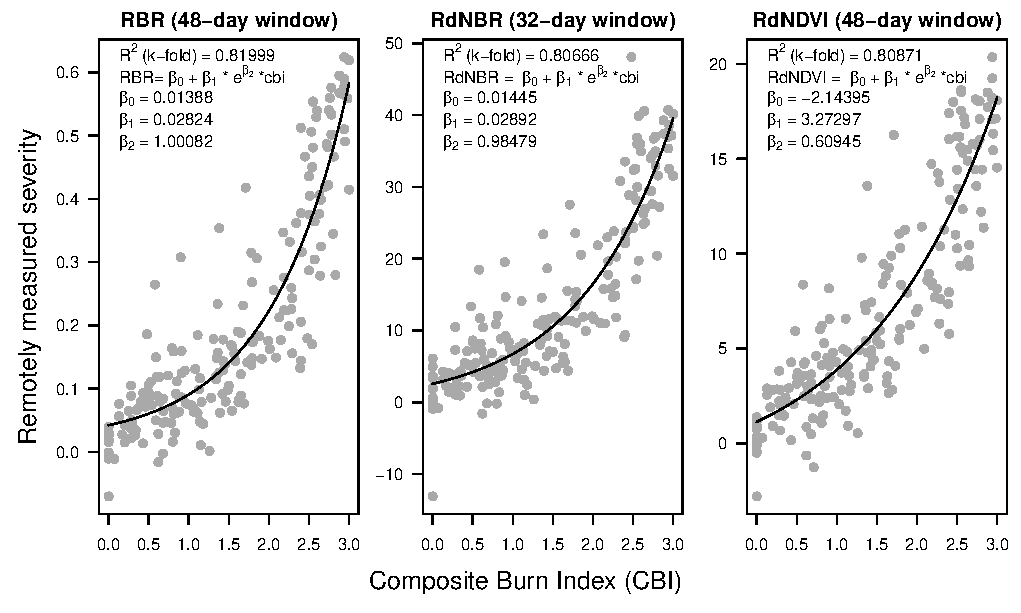
\includegraphics[width=6.00000in]{figure/chap01/remote-sensed-severity-calibration.pdf}
\caption{Three top performing remotely-sensed severity metrics based on
5-fold cross validation (relative burn ratio, 48-day window, bicubic
interpolation; relative delta normalized burn ratio, 32-day window,
bilinear interpolation; and relative delta normalized difference
vegetation index, 48-day window, bilinear interpolation) calculated
using new automated image collation algorithms, calibrated to 208 field
measures of fire severity (composite burn index). See Supplemental Table
1 for performance of all tested models.}
\end{figure}
Based on these model comparisons, we used the relative burn ratio (RBR)
calculated using a 48-day time window before the fire and bicubic
interpolation as our metric of severity. We created the boolean response
variable representing whether the sampled point burned at high-severity
or not by determining whether the RBR exceeded 0.282, the threshold for
high-severity derived using the non-linear relationship in Equation 1.1
(Figure 1.1).

\subsection{Neighborhood size effect}\label{neighborhood-size-effect}
\begin{longtable}[]{@{}ccccccc@{}}
\caption{Comparison of four models described in Eq.
\ref{eq-severity-model} using different neighborhood sizes for
calculating forest structural variability (standard deviation of NDVI
within the neighborhood), neighborhood mean NDVI, and topographic
roughness. LOO is a measure of a model's predictive accuracy (with lower
values corresponding to more accurate prediction) and is calculated as
-2 times the expected log pointwise predictive density (elpd) for a new
dataset (Vehtari et al. \protect\hyperlink{ref-vehtari2017}{2017}).
\(\Delta\)LOO is the difference between a model's LOO and the lowest LOO
in a set of models (i.e., the model with the best predictive accuracy).
The Bayesian \(R^2\) is a `data-based estimate of the proportion of
variance explained for new data' (Gelman et al.
\protect\hyperlink{ref-gelman2018}{2018}). Note that Bayesian \(R^2\)
values are conditional on the model so shouldn't be compared across
models, though they can be informative about a single model at a
time.}\tabularnewline
\toprule
\begin{minipage}[b]{0.06\columnwidth}\centering\strut
Model\strut
\end{minipage} & \begin{minipage}[b]{0.17\columnwidth}\centering\strut
Neighborhood size for variability measure\strut
\end{minipage} & \begin{minipage}[b]{0.09\columnwidth}\centering\strut
LOO (-2*elpd)\strut
\end{minipage} & \begin{minipage}[b]{0.11\columnwidth}\centering\strut
\(\Delta\) LOO to best model\strut
\end{minipage} & \begin{minipage}[b]{0.11\columnwidth}\centering\strut
SE of \(\Delta\) LOO\strut
\end{minipage} & \begin{minipage}[b]{0.16\columnwidth}\centering\strut
LOO model weight (\%)\strut
\end{minipage} & \begin{minipage}[b]{0.11\columnwidth}\centering\strut
Bayesian R\textsuperscript{2}\strut
\end{minipage}\tabularnewline
\midrule
\endfirsthead
\toprule
\begin{minipage}[b]{0.06\columnwidth}\centering\strut
Model\strut
\end{minipage} & \begin{minipage}[b]{0.17\columnwidth}\centering\strut
Neighborhood size for variability measure\strut
\end{minipage} & \begin{minipage}[b]{0.09\columnwidth}\centering\strut
LOO (-2*elpd)\strut
\end{minipage} & \begin{minipage}[b]{0.11\columnwidth}\centering\strut
\(\Delta\) LOO to best model\strut
\end{minipage} & \begin{minipage}[b]{0.11\columnwidth}\centering\strut
SE of \(\Delta\) LOO\strut
\end{minipage} & \begin{minipage}[b]{0.16\columnwidth}\centering\strut
LOO model weight (\%)\strut
\end{minipage} & \begin{minipage}[b]{0.11\columnwidth}\centering\strut
Bayesian R\textsuperscript{2}\strut
\end{minipage}\tabularnewline
\midrule
\endhead
\begin{minipage}[t]{0.06\columnwidth}\centering\strut
1\strut
\end{minipage} & \begin{minipage}[t]{0.17\columnwidth}\centering\strut
90m x 90m\strut
\end{minipage} & \begin{minipage}[t]{0.09\columnwidth}\centering\strut
40786\strut
\end{minipage} & \begin{minipage}[t]{0.11\columnwidth}\centering\strut
0\strut
\end{minipage} & \begin{minipage}[t]{0.11\columnwidth}\centering\strut
NA\strut
\end{minipage} & \begin{minipage}[t]{0.16\columnwidth}\centering\strut
100\strut
\end{minipage} & \begin{minipage}[t]{0.11\columnwidth}\centering\strut
0.299\strut
\end{minipage}\tabularnewline
\begin{minipage}[t]{0.06\columnwidth}\centering\strut
2\strut
\end{minipage} & \begin{minipage}[t]{0.17\columnwidth}\centering\strut
150m x 150m\strut
\end{minipage} & \begin{minipage}[t]{0.09\columnwidth}\centering\strut
40842\strut
\end{minipage} & \begin{minipage}[t]{0.11\columnwidth}\centering\strut
56.03\strut
\end{minipage} & \begin{minipage}[t]{0.11\columnwidth}\centering\strut
14.69\strut
\end{minipage} & \begin{minipage}[t]{0.16\columnwidth}\centering\strut
0\strut
\end{minipage} & \begin{minipage}[t]{0.11\columnwidth}\centering\strut
0.298\strut
\end{minipage}\tabularnewline
\begin{minipage}[t]{0.06\columnwidth}\centering\strut
3\strut
\end{minipage} & \begin{minipage}[t]{0.17\columnwidth}\centering\strut
210m x 210m\strut
\end{minipage} & \begin{minipage}[t]{0.09\columnwidth}\centering\strut
40883\strut
\end{minipage} & \begin{minipage}[t]{0.11\columnwidth}\centering\strut
96.87\strut
\end{minipage} & \begin{minipage}[t]{0.11\columnwidth}\centering\strut
20.94\strut
\end{minipage} & \begin{minipage}[t]{0.16\columnwidth}\centering\strut
0\strut
\end{minipage} & \begin{minipage}[t]{0.11\columnwidth}\centering\strut
0.297\strut
\end{minipage}\tabularnewline
\begin{minipage}[t]{0.06\columnwidth}\centering\strut
4\strut
\end{minipage} & \begin{minipage}[t]{0.17\columnwidth}\centering\strut
270m x 270m\strut
\end{minipage} & \begin{minipage}[t]{0.09\columnwidth}\centering\strut
40912\strut
\end{minipage} & \begin{minipage}[t]{0.11\columnwidth}\centering\strut
125.9\strut
\end{minipage} & \begin{minipage}[t]{0.11\columnwidth}\centering\strut
24.73\strut
\end{minipage} & \begin{minipage}[t]{0.16\columnwidth}\centering\strut
0\strut
\end{minipage} & \begin{minipage}[t]{0.11\columnwidth}\centering\strut
0.297\strut
\end{minipage}\tabularnewline
\bottomrule
\end{longtable}
The model with the best out-of-sample prediction accuracy assessed by
leave-one-out cross validation was the model fit using the smallest
neighborhood size for the variability of forest structure (standard
deviation of neighborhood NDVI), the mean of neighborhood NDVI, and the
terrain roughness (standard deviation of elevation) (Table 1.1). Model
weighting based on the LOO score suggests 100\% of the model weight
belongs to the model using the smallest neighborhood size window.

\subsection{Effects of prefire vegetation density, 100-hour fuel
moisture, potential annual heat load, and topographic roughness on
wildfire
severity}\label{effects-of-prefire-vegetation-density-100-hour-fuel-moisture-potential-annual-heat-load-and-topographic-roughness-on-wildfire-severity}
\begin{figure}
\centering
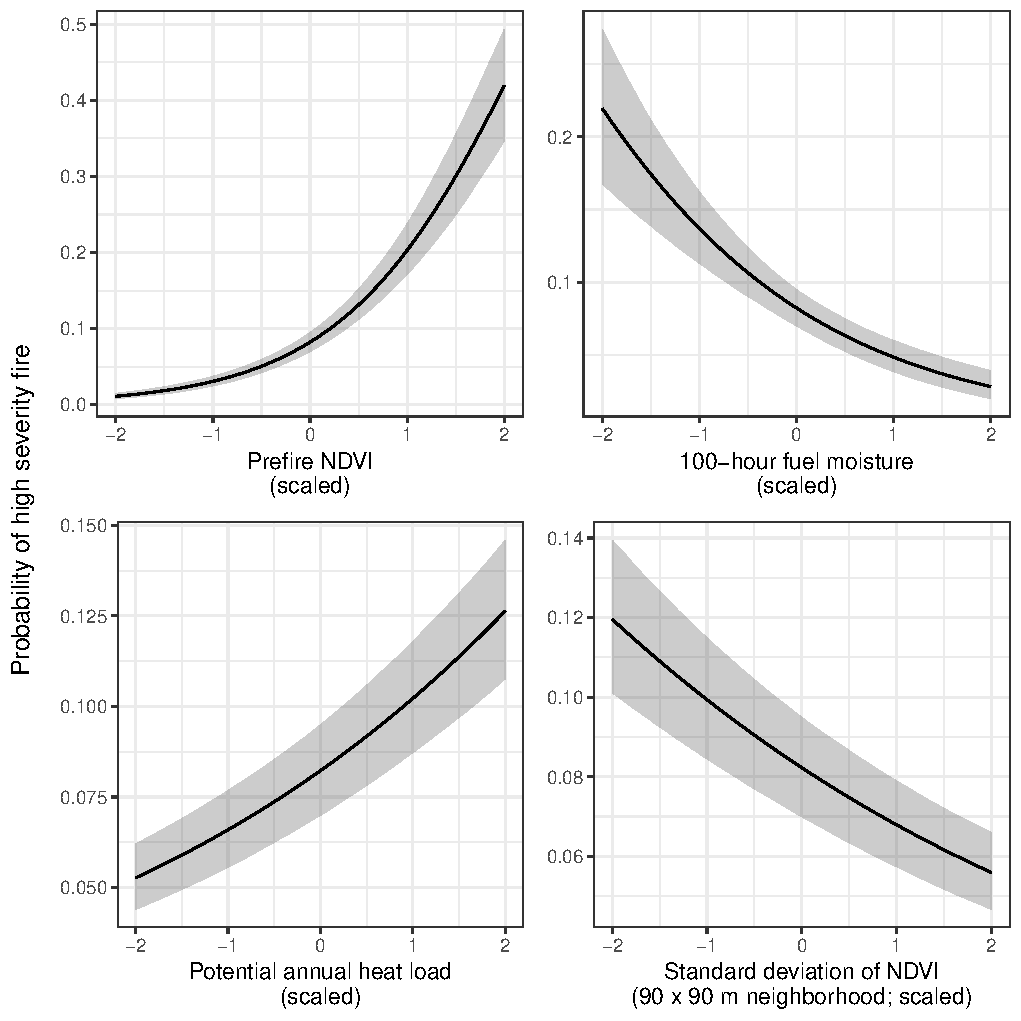
\includegraphics[width=6.00000in]{figure/chap01/prob-hi-sev-main-effects-credible-intervals.pdf}
\caption{The main effects and 95\% credible intervals of the covariates
having the strongest relationships with the probability of high-severity
fire. All depicted relationships derive from the model using the 90m x
90m neighborhood size window for neighborhood standard deviation of
NDVI, neighborhood mean of NDVI, and topographic roughness, as this was
the best performing model of the four neighborhood sizes tested. The
effect sizes of these covariates were similar for each neighborhood size
tested.}
\end{figure}
We report the results from fitting the model described in Equation 1.2
using the smallest neighborhood size (90m x 90m) because this was the
best performing model (see above) and because the size and magnitude of
estimated coefficients were similar across neighborhood sizes (Supp.
Table 2).

We found that the strongest influence on the probability of a forested
area burning at high-severity was the density of the vegetation, as
measured by the prefire NDVI at that central pixel. A greater prefire
NDVI led to a greater probability of high-severity fire
(\(\beta_{\text{prefire\_ndvi}}=\) 1.044; 95\% CI: {[}0.911, 1.174{]});
Figure 1.2). There was a strong negative relationship between 100-hour
fuel moisture and wildfire severity such that increasing 100-hour fuel
moisture was associated with a reduction in the probability of a
high-severity wildfire (\(\beta_{\text{fm100}}=\) -0.569; 95\% CI:
{[}-0.71, -0.423{]}) (Figure 1.2). Potential annual heat load, which
integrates aspect, slope, and latitude, also had a strong positive
relationship with the probability of a high-severity fire. Areas that
were located on southwest facing sloped terrain at lower latitudes had
the highest potential annual heat load, and they were more likely to
burn at high-severity (\(\beta_{\text{pahl}}=\) 0.239; 95\% CI:
{[}0.208, 0.271{]}) Figure 1.2). We found no effect of local topographic
roughness on wildfire severity
(\(\beta_{\text{topographic\_roughness}}=\) -0.01; 95\% CI: {[}-0.042,
0.022{]}). We found a negative effect of the prefire neighborhood mean
NDVI on the probability of a pixel burning at high-severity
(\(\beta_{\text{nbhd\_mean\_NDVI}}=\) -0.14; 95\% CI: {[}-0.278,
0.002{]}). This is in contrast to the positive effect of the prefire
NDVI of the pixel itself.

There was also a strong negative interaction between the neighborhood
mean NDVI and the prefire NDVI of the central pixel
(\(\beta_{\text{nbhd\_mean\_NDVI*prefire\_NDVI}}\) -0.573; 95\% CI:
{[}-0.62, -0.526{]}).

\subsection{Effect of variability of vegetation structure on wildfire
severity}\label{effect-of-variability-of-vegetation-structure-on-wildfire-severity}

We found strong evidence for a negative effect of variability of
vegetation structure on the probability of a high-severity wildfire
(\(\beta_{\text{nbhd\_stdev\_NDVI}}=\) -0.208; 95\% CI: {[}-0.247,
-0.17{]}); Figure 1.2). We also found significant interactions between
variability of vegetation structure and prefire NDVI
\(\beta_{\text{nbhd\_stdev\_NDVI*prefire\_NDVI}}=\) 0.125; 95\% CI:
{[}0.029, 0.218{]}) as well as between variability of vegetation
structure and neighborhood mean NDVI
(\(\beta_{\text{nbhd\_stdev\_NDVI*nbhd\_mean\_NDVI}}=\) -0.129; 95\% CI:
{[}-0.223, -0.034{]}).

\section{Discussion}\label{discussion}

Broad-extent, fine-grain, spatially-explicit analyses of whole
ecosystems are key to illuminating macroecological phenomena (Heffernan
et al. \protect\hyperlink{ref-heffernan2014}{2014}). We used a powerful,
cloud-based geographic information system and data repository, Google
Earth Engine, as a `macroscope' (Beck et al.
\protect\hyperlink{ref-beck2012}{2012}) to study feedbacks between
vegetation structure and wildfire disturbance in yellow
pine/mixed-conifer forests of California's Sierra Nevada mountain range.
With this approach, we reveal and quantify general features of this
forest system, and gain deeper insights into the mechanisms underlying
its function.

\subsection{Factors influencing the probability of high-severity
wildfire}\label{factors-influencing-the-probability-of-high-severity-wildfire}

We found that the strongest influence on the probability of
high-severity wildfire was prefire NDVI. Greater NDVI corresponds to
high canopy cover and vegetation density (Rouse et al.
\protect\hyperlink{ref-rouse1973}{1973}) which translate directly to
live fuel loads in the forest canopy and can increase high severity fire
(Parks et al. \protect\hyperlink{ref-parks2018}{2018}). Critically,
overstory canopy cover and density also correlate with surface fuel
loads (Lydersen et al. \protect\hyperlink{ref-lydersen2015}{2015},
Collins et al. \protect\hyperlink{ref-collins2016}{2016}), which play a
larger role in driving high severity fire compared to canopy fuel loads
in these forests (Stephens et al.
\protect\hyperlink{ref-stephens2012a}{2012}). Thus NDVI is likely a
strong predictor of fire severity because it is correlated with both
surface fuel loads and canopy live fuel density.

We found a strong positive effect of potential annual heat load as well
as a strong negative effect of 100-hour fuel moisture, results which
corroborates similar studies (Parks et al.
\protect\hyperlink{ref-parks2018}{2018}). Some work has shown that
terrain ruggedness (Holden et al.
\protect\hyperlink{ref-holden2009}{2009}), and particularly
coarser-scale terrain ruggedness (Dillon et al.
\protect\hyperlink{ref-dillon2011}{2011}), is an important predictor of
wildfire severity, but we found no effect using our measure of terrain
ruggedness.

Critically, we found a strong negative effect of forest structural
variability on wildfire severity that was opposite in direction but
similar in magnitude to the effect of potential annual heat load. Just
as the positive effect of NDVI is likely driven by surface fuel loads,
the negative effect of variability in NDVI (our measure of structural
variability), is likely driven by discontinuity in surface fuel loads,
which can reduce the probability of initiation and spread of
tree-killing crown fires (Wagner
\protect\hyperlink{ref-wagner1977}{1977}, Agee and ForestResourcesU
\protect\hyperlink{ref-agee1996}{1996}, Graham et al.
\protect\hyperlink{ref-graham2004}{2004}, Agee and Skinner
\protect\hyperlink{ref-agee2005}{2005}).

\subsection{Feedback between forest structural variability and wildfire
severity}\label{feedback-between-forest-structural-variability-and-wildfire-severity}

This system-wide inverse relationship between structural variability and
wildfire severity closes a feedback that links past and future fire
behavior via forest structure. Frequent, mixed-severity wildfire
generates variable forest structure (North et al.
\protect\hyperlink{ref-north2009a}{2009}, Larson and Churchill
\protect\hyperlink{ref-larson2012}{2012}, Malone et al.
\protect\hyperlink{ref-malone2018}{2018}), which in turn, as we
demonstrate, dampens the severity of future fire. In contrast, exclusion
of wildfire homogenizes forest structure and increases the probability
that a fire, when it occurs, will produce large, contiguous patches of
overstory mortality (Stevens et al.
\protect\hyperlink{ref-stevens2017}{2017}, Steel et al.
\protect\hyperlink{ref-steel2018}{2018}). The proportion and spatial
configuration of fire severity in fire-prone forests are key
determinants of their long-term persistence (Stevens et al.
\protect\hyperlink{ref-stevens2017}{2017}, Steel et al.
\protect\hyperlink{ref-steel2018}{2018}). Lower-severity fire or
scattered patches of higher-severity fire reduce the risk of conversion
to a non-forest vegetation type (Stevens et al.
\protect\hyperlink{ref-stevens2017}{2017}, Walker et al.
\protect\hyperlink{ref-walker2018}{2018}), while prospects for forest
regeneration are bleak when high-severity patch sizes are much larger
than the natural range of variation for the system (Wagtendonk
\protect\hyperlink{ref-wagtendonk2006}{2006}, Stephens et al.
\protect\hyperlink{ref-stephens2009}{2009}, Millar and Stephenson
\protect\hyperlink{ref-millar2015}{2015}, Coppoletta et al.
\protect\hyperlink{ref-coppoletta2016}{2016}, Safford and Stevens
\protect\hyperlink{ref-safford2017}{2017}, Miller and Safford
\protect\hyperlink{ref-miller2017}{2017}, Stevens et al.
\protect\hyperlink{ref-stevens2017}{2017}). Thus, the
forest-structure-mediated feedback between past and future fire severity
underlies the resilience of the Sierra Nevada yellow pine/mixed-conifer
system.

\subsection{Neighborhood size}\label{neighborhood-size}

We found that the effect of a forest patch's neighborhood
characteristics on the probability of high-severity fire was strongest
at the smallest neighborhood size that we tested, 90m x 90m. This
suggests that the moderating effect of variability in vegetation
structure on fire severity is a very local phenomenon. This corroborates
work by Safford et al. (\protect\hyperlink{ref-safford2012}{2012}), who
found that crown fires (with high tree killing potential) were almost
always reduced to surface fires (with low tree killing potential) within
70m of entering an fuel reduction treatment area.

At a landscape level, forest treatments that reduce fuel loads and
increase structural variability can be effective at reducing fire
severity across broader spatial scales (Stephens et al.
\protect\hyperlink{ref-stephens2009}{2009}). This may reflect that
severity patterns for a whole fire are an emergent property of very
local interactions between forest structure and fire behavior. Some work
suggests that the scale of these interactions may depend on even
broader-scale effects of fire weather, with small-scale variability
failing to influence fire behavior under extreme conditions (Peters et
al. \protect\hyperlink{ref-peters2004}{2004}, Lydersen et al.
\protect\hyperlink{ref-lydersen2014}{2014}), though we did not detect
such an interaction. The notion of emergent patterns of severity arising
from local effects of vegetation structure is supported by work on fuel
reduction treatments, which suggests that fire behavior can be readily
modified with forest structural changes to only 20\% (when strategically
located) to 60\% (when randomly located) of the landscape (Graham et al.
\protect\hyperlink{ref-graham2004}{2004}).

\subsection{Correlation between covariates and
interactions}\label{correlation-between-covariates-and-interactions}

Unexpectedly, we found a strong interaction between the prefire NDVI at
a pixel and its neighborhood mean NDVI. These two variables are strongly
correlated (\(\text{Spearman's }\rho=\) 0.97), so the general effect of
this interaction is to dampen the dominating effect of prefire NDVI.
Thus, though the marginal effect of prefire NDVI on the probability of
high-severity fire is still positive and large, its real-world effect
might be more comparable to other modeled covariates when including the
negative main effect of neighborhood mean NDVI, the negative interaction
effect of prefire NDVI and neighborhood mean NDVI, and their tendency to
covary (compare the real-world effect of vegetation density:
\(\beta_{\text{prefire\_ndvi}}+\beta_{\text{nbhd\_mean\_NDVI}}+\beta_{\text{nbhd\_mean\_NDVI*prefire\_NDVI}}=\)
0.331, to the effect of 100-hour fuel moisture, which becomes the effect
with the greatest magnitude: \(\beta_{\text{fm100}}=\) -0.569).

In the few cases when prefire NDVI and the neighborhood mean NDVI
contrast, there is an overall effect of increasing the probability of
high-severity fire. When prefire NDVI at the central pixel is high and
the neighborhood NDVI is low (e.g., an isolated vegetation patch;
Supplemental Fig. 2), the probability of high-severity fire is expected
to dramatically increase. When prefire NDVI at the central pixel is low
and the neighborhood NDVI is high (e.g., a hole in the center of an
otherwise dense forest; Supplemental Fig. 2), the probability of
high-severity fire at that central pixel is still expected to be fairly
high even though there is limited vegetation density (see Supplemental
Fig. 2). In these forest NDVI datasets, when these variables do
decouple, they tend to do so in the ``hole in the forest'' case and lead
to a greater probability of high-severity fire at the central pixel
despite the lower vegetation density there. This can perhaps be
explained if the consistently high vegetation density in a local
neighborhood-- itself more likely to burn at high-severity-- exerts a
contagious effect on the central pixel, raising its probability of
burning at high-severity regardless of how much fuel might be there to
burn.

\subsection{A new approach to remotely sensing wildfire
severity}\label{a-new-approach-to-remotely-sensing-wildfire-severity}

We developed a new approach to calculating wildfire severity leveraging
the cloud-based data catalog, the large parallel processing system, and
the distribution of computation tasks in Google Earth Engine to enable
rapid high-throughput analyses of earth observation data (Gorelick et
al. \protect\hyperlink{ref-gorelick2017}{2017}). Our programmatic
assessment of wildfire severity across the 972 Sierra Nevada yellow
pine/mixed-conifer fires in the FRAP perimeter database, which required
fetching thousands of Landsat images and performing dozens of
calculations across them, was automated and took less than an hour to
complete. We found that the relative burn ratio (RBR) calculated using
prefire Landsat images collected over a 48-day period prior to the fire
and postfire Landsat images collected over a 48-day period one year
after the prefire images validated the best with ground-based severity
measurements (composite burn index; CBI). Further, we found that this
method was robust to a wide range of severity metrics, time windows, and
interpolation techniques.

Most efforts to calculate severity from satellite data rely on hand
curation of a single prefire and a single postfire image (Miller and
Thode \protect\hyperlink{ref-miller2007}{2007}, Miller et al.
\protect\hyperlink{ref-miller2009a}{2009}, De Santis et al.
\protect\hyperlink{ref-desantis2010}{2010}, Cansler and McKenzie
\protect\hyperlink{ref-cansler2012}{2012}, Veraverbeke and Hook
\protect\hyperlink{ref-veraverbeke2013}{2013}, Parks et al.
\protect\hyperlink{ref-parks2014a}{2014}, Prichard and Kennedy
\protect\hyperlink{ref-prichard2014}{2014}, Edwards et al.
\protect\hyperlink{ref-edwards2018}{2018}, Fernández-García et al.
\protect\hyperlink{ref-fernandez-garcia2018}{2018}). Recently, Parks et
al. (\protect\hyperlink{ref-parks2018}{2018}) found that using a
composite of several prefire images and several postfire images to
detect fire impacts performed at least as well as using a single pre-
and postfire image. Using composite images also facilitated automated
image fetching. Parks et al. (\protect\hyperlink{ref-parks2018}{2018})
used 3- to 4-month windows during pre-specified times of the year
(depending on the fire's region) to collate pre- and postfire imagery
one year before the fire and one year after. In contrast, we tested
multiple time window lengths based on the fire start date regardless of
when it burned during the year. Basing our pre- and postfire image
fetching on fixed lengths of time since the fire start date standardized
the amount of time elapsed in each severity assessment. Our best
remotely sensed severity configuration used a much shorter time window
compared to Parks et al. (\protect\hyperlink{ref-parks2018}{2018}) (48
days versus 3 to 4 months), which likely balanced an incorporation of
enough imagery to be representative of the pre- and postfire vegetation
conditions but not so many images that different phenological conditions
across the time window added noise to each composite.

Many algorithms have been developed to measure fire effects on
vegetation in an attempt to better correspond to field data (Key and
Benson \protect\hyperlink{ref-key2006}{2006}, Miller and Thode
\protect\hyperlink{ref-miller2007}{2007}, Parks et al.
\protect\hyperlink{ref-parks2014a}{2014}). We found that several other
remotely sensed measures of severity, including one based on NDVI that
is rarely deployed, validated nearly as well with ground-based data as
the best configuration (RBR calculated using a 48-day time window). We
echo the conclusion of Zhu et al.
(\protect\hyperlink{ref-zhu2006}{2006}) that the validation of
differences between pre- and postfire NDVI to field measured severity
data, which uses near infrared reflectance, is comparable to validation
using more commonly used severity metrics (e.g., RdNBR and RBR) that
rely on short wave infrared reflectance. One immediately operational
implication of this is that the increasing availability of low-cost
small unhumanned aerial systems (sUAS a.k.a. drones) and
near-infrared-detecting imagers (e.g., those used for agriculture
monitoring) may be used to reliably measure wildfire severity at very
high spatial resolutions.

\subsection{Conclusions}\label{conclusions}

While the severity of a wildfire in any given place is controlled by
many variables, we have presented strong evidence that, across large
areas of forest, variable forest structure generally makes yellow
pine/mixed-conifer forest in the Sierra Nevada more resistant to this
inevitable disturbance. It has been well-documented that frequent,
low-severity wildfire maintains forest structural variability. Here, we
demonstrate a system-wide reciprocal effect suggesting that greater
local-scale variability of vegetation structure makes fire-prone, dry
forests more resilient to wildfire and may increase the probability of
their long-term persistence.

\section{Material and Methods}\label{material-and-methods}

\subsection{Study system}\label{study-system}
\begin{figure}
\centering
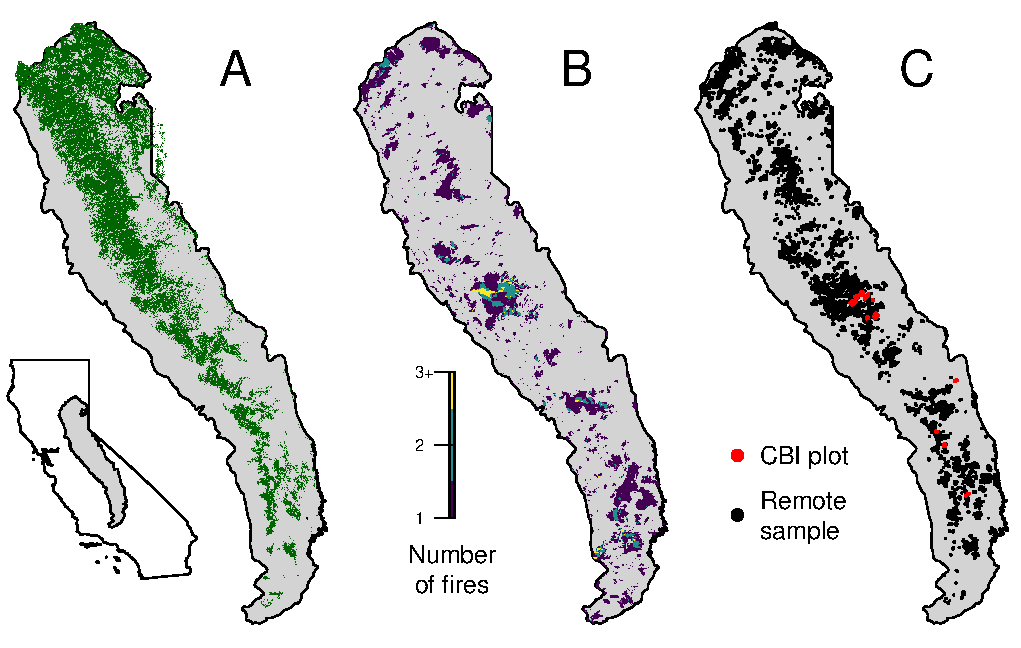
\includegraphics[width=6.00000in]{figure/chap01/study-geographic-setting.pdf}
\caption{Geographic setting of the study. A) Location of yellow
pine/mixed-conifer forests as designated by the Fire Return Interval
Departure (FRID) product which, among other things, describes the
potential vegetation in an area based on the pre-Euroamerican settlement
fire regime. B) Locations of all fires covering greater than 4 hectares
that burned in yellow pine/mixed-conifer forest between 1984 and 2017 in
the Sierra Nevada mountain range of California according to the State of
California Fire Resource and Assessment Program database, the most
comprehensive database of fire perimeters of its kind. Colors indicate
how many fire perimeters overlapped a given pixel within the study time
period. C) (red) Locations of 208 composite burn index (CBI) ground
plots used to calibrate the remotely sensed measures of severity.
(black) Locations of random samples drawn from 972 unique fires depicted
in panel B that were in yellow pine/mixed-conifer forest as depicted in
panel A, and which were designated as ``burned'' by exceeding a
threshold relative burn ratio (RBR) determined by calibrating the
algorithm presented in this study with ground-based CBI measurements.}
\end{figure}
Our study assesses the effect of vegetation structure on wildfire
severity in the Sierra Nevada mountain range of California in yellow
pine/mixed-conifer forests (Figure 1.3). This system is dominated by a
mixture of conifer species including ponderosa pine (\emph{Pinus
ponderosa}), sugar pine (\emph{Pinus lambertiana}), incense-cedar
(\emph{Calocedrus decurrens}), Douglas-fir (\emph{Pseudotsuga
menziesii}), white fir (\emph{Abies concolor}), and red fir (\emph{Abies
magnifica}), angiosperm trees primarily including black oak
(\emph{Quercus kelloggii}), as well as shrubs (Safford and Stevens
\protect\hyperlink{ref-safford2017}{2017}). We considered ``yellow
pine/mixed-conifer forest'' to be all areas designated as a yellow pine,
dry mixed-conifer, or moist mixed-conifer pre-settlement fire regime
(PFR) in the USFS Fire Return Interval Departure database
(\url{https://www.fs.usda.gov/detail/r5/landmanagement/gis/?cid=STELPRDB5327836}),
which reflects potential vegetation and is less sensitive to recent land
cover change (Steel et al. \protect\hyperlink{ref-steel2018}{2018}). We
considered the Sierra Nevada region to be the area within the Sierra
Nevada Foothills, the High Sierra Nevada, and the Tehachapi Mountain
Area Jepson ecoregions (JepsonFloraProject
\protect\hyperlink{ref-jepsonfloraproject2016}{2016}).

\subsection{A new approach to remotely sensing wildfire
severity}\label{a-new-approach-to-remotely-sensing-wildfire-severity-1}

We measured forest vegetation characteristics and wildfire severity
using imagery from the Landsat series of satellites (Miller and Thode
\protect\hyperlink{ref-miller2007}{2007}, Eidenshink et al.
\protect\hyperlink{ref-eidenshink2007}{2007}) with radiometric
correction post-processing (Masek et al.
\protect\hyperlink{ref-masek2006}{2006}, Vermote et al.
\protect\hyperlink{ref-vermote2016}{2016}, USGS
\protect\hyperlink{ref-usgs2017a}{2017}\protect\hyperlink{ref-usgs2017a}{a},
\protect\hyperlink{ref-usgs2017}{2017}\protect\hyperlink{ref-usgs2017}{b}).
Landsat satellites image the entire Earth approximately every 16 days
with a 30m pixel resolution. We used Google Earth Engine, a massively
parallel cloud-based geographic information system and image hosting
platform, for all image collation and processing (Gorelick et al.
\protect\hyperlink{ref-gorelick2017}{2017}).

We calculated wildfire severity for the most comprehensive digital
record of fire perimeters in California: The California Department of
Forestry and Fire Protection, Fire and Resource Assessment Program
(FRAP) fire perimeter database
(\url{http://frap.fire.ca.gov/projects/fire_data/fire_perimeters_index}).
The FRAP database includes all known fires that covered more than 4
hectares, compared to the current standard severity database in this
region which only includes fires covering greater than 80 hectares
(Miller and Thode \protect\hyperlink{ref-miller2007}{2007}, Miller et
al. \protect\hyperlink{ref-miller2012}{2012}, Miller and Safford
\protect\hyperlink{ref-miller2012a}{2012}, Steel et al.
\protect\hyperlink{ref-steel2018}{2018}). Using the FRAP database of
fire perimeters, we quantified fire severity within each perimeter of
972 wildfires in the Sierra Nevada yellow pine/mixed-conifer forest that
burned between 1984 and 2017. Our approach more than doubles the number
of fire events represented from 430 to 972, though only increases the
total burned area represented from 7.44e+05 to 7.69e+05 hectares because
most of the additional fires are small. We use a consistent algorithmic
approach to calculate fire severity across all fires, avoiding
subjective judgements that some previous approaches have used to
characterize severity separately for each fire.

\subsubsection{Fetching and processing pre- and postfire
imagery}\label{fetching-and-processing-pre--and-postfire-imagery}

For each fire perimeter, we fetched a time series of prefire Landsat
images starting the day before the fire alarm date and extending
backward in time by a user-defined time window. An analogous postfire
time series of Landsat imagery was fetched exactly one year after the
date range used to filter the prefire collection. We tested 4 time
windows: 16, 32, 48, or 64 days which were chosen to ensure that at
least 1, 2, 3, or 4 Landsat images were captured by the date ranges
(Supplemental Fig. 1). The Landsat archive we filtered included imagery
from Landsat 4, 5, 7, and 8, so each pre- and postfire image collection
may contain a mix of scenes from different satellite sources to enhance
coverage. For each image in the pre- and postfire image collections, we
masked pixels that were not clear (i.e., clouds, cloud shadows, snow,
and water) using the CFMask algorithm (Foga et al.
\protect\hyperlink{ref-foga2017}{2017}).

For each Landsat image in the prefire and postfire collections, we
calculated standard indices that capture vegetation cover and fire
effects such as charring. Normalized difference vegetation index (NDVI)
correlates with vegetation density, canopy cover, and leaf area index
(Rouse et al. \protect\hyperlink{ref-rouse1973}{1973}). Normalized burn
ratio (NBR) and normalized burn ratio version 2 (NBR2) respond strongly
to fire effects on vegetation (García and Caselles
\protect\hyperlink{ref-garcia1991}{1991}, Key and Benson
\protect\hyperlink{ref-key2006}{2006}, USGS
\protect\hyperlink{ref-usgs2017}{2017}\protect\hyperlink{ref-usgs2017}{b},
\protect\hyperlink{ref-usgs2017a}{2017}\protect\hyperlink{ref-usgs2017a}{a},
Hawbaker et al. \protect\hyperlink{ref-hawbaker2017}{2017}) (Equations
in Supplemental Methods).

We composited each prefire image collection (including the pixel values
representing NDVI, NBR, and NBR2) into a single prefire image and each
postfire image collection into a single postfire image, by calculating
the median of the unmasked values on a per-pixel basis across the stack
of images in each pre- and postfire collection. Composite pre- and
postfire images can be successfully used to measure wildfire severity
instead of using raw, individual images (Parks et al.
\protect\hyperlink{ref-parks2018}{2018}).

We composited each pre- and postfire image collection (including the
pixel values representing NDVI, NBR, and NBR2) into a single pre- and
postfire image using a median reducer, which calculated the median of
the unmasked values on a per-pixel basis across the stack of images in
each collection. Composite pre- and postfire images can be successfully
used to measure wildfire severity instead of using raw, individual
images (Parks et al. \protect\hyperlink{ref-parks2018}{2018}).

\subsubsection{Calculating wildfire
severity}\label{calculating-wildfire-severity}

Using the compositing approach, we calculated the most commonly used
metrics of remotely-sensed wildfire severity to validate against
ground-based data: the relative burn ratio (RBR) (Parks et al.
\protect\hyperlink{ref-parks2014a}{2014}), the delta normalized burn
ratio (dNBR) (Miller and Thode \protect\hyperlink{ref-miller2007}{2007},
Eidenshink et al. \protect\hyperlink{ref-eidenshink2007}{2007}), the
relative delta normalized burn ratio (RdNBR) (Miller and Thode
\protect\hyperlink{ref-miller2007}{2007}, Miller and Safford
\protect\hyperlink{ref-miller2012a}{2012}), the delta normalized burn
ratio 2 (dNBR2) (Hawbaker et al.
\protect\hyperlink{ref-hawbaker2017}{2017}), the relative delta
normalized burn ratio 2 (RdNBR2), and the delta normalized difference
vegetation index (dNDVI) (Eidenshink et al.
\protect\hyperlink{ref-eidenshink2007}{2007}). We also calculate a new,
analogous metric to the RdNBR using NDVI-- the relative delta normalized
difference vegetation index (RdNDVI). We calculated the delta severity
indices (dNBR, dNBR2, dNDVI) without multiplying by a rescaling constant
(e.g., we did not multiply the result by 1000 as in Miller and Thode
(\protect\hyperlink{ref-miller2007}{2007})). Following Reilly et al.
(\protect\hyperlink{ref-reilly2017}{2017}), we did not correct the delta
indices using a phenological offset value, as our approach implicitly
accounts for phenology by incorporating multiple cloud-free images
across the same time window both before the fire and one year later.
(Full equations can be found in the Supplemental Methods)

Example algorithm outputs are shown in Figure 1.4.
\begin{figure}
\centering
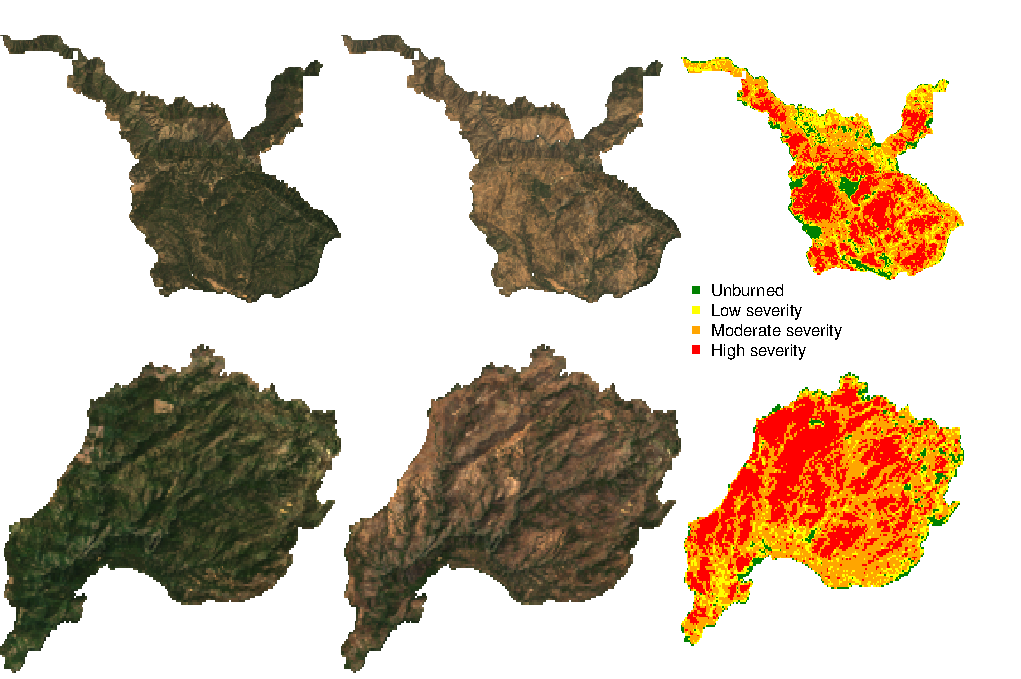
\includegraphics[width=6.00000in]{figure/chap01/pre-post-rbr.pdf}
\caption{Example algorithm outputs for the Hamm Fire of 1987 (top half)
and the American Fire of 2013 (bottom half) showing: prefire true color
image (left third), postfire true color image (center third), relative
burn ratio (RBR) calculation using a 48-day image collation window
before the fire and one year later (right third). For visualization
purposes, these algorithm outputs have been resampled to a resolution of
100m x 100m from their original resolution of 30m x 30m. Data used for
analyses were sampled from the outputs at the original resolution.}
\end{figure}
\subsubsection{Calibrating remotely-sensed wildfire severity with
field-measured wildfire
severity}\label{calibrating-remotely-sensed-wildfire-severity-with-field-measured-wildfire-severity}

We calibrated our remotely-sensed measure of wildfire severity with 208
field measures of overstory tree mortality from two previously published
studies (Zhu et al. \protect\hyperlink{ref-zhu2006}{2006}, Sikkink et
al. \protect\hyperlink{ref-sikkink2013}{2013}) (Figure 1.3). The
Composite Burn Index (CBI) is a metric of vegetation mortality across
several vertical vegetation strata within a 30m diameter field plot (Key
and Benson \protect\hyperlink{ref-key2006}{2006}). The CBI ranges from 0
(no fire impacts) to 3 (very high fire impacts), and has a long history
of use as a standard for calibrating remotely-sensed severity data (Key
and Benson \protect\hyperlink{ref-key2006}{2006}, Miller and Thode
\protect\hyperlink{ref-miller2007}{2007}, Miller et al.
\protect\hyperlink{ref-miller2009a}{2009}, Cansler and McKenzie
\protect\hyperlink{ref-cansler2012}{2012}, Parks et al.
\protect\hyperlink{ref-parks2014a}{2014},
\protect\hyperlink{ref-parks2018}{2018}, Prichard and Kennedy
\protect\hyperlink{ref-prichard2014}{2014}). Following Miller and Thode
(\protect\hyperlink{ref-miller2007}{2007}), Miller et al.
(\protect\hyperlink{ref-miller2009a}{2009}), Parks et al.
(\protect\hyperlink{ref-parks2014a}{2014}), and Parks et al.
(\protect\hyperlink{ref-parks2018}{2018}), we fit a non-linear model to
each remotely-sensed severity metric of the following form:
\begin{enumerate}
\def\labelenumi{(\arabic{enumi})}
\tightlist
\item
  \(\label{eq-cbi-calibration} \text{remote\_severity} = \beta_0 + \beta_1 e^{\beta_2 \text{cbi\_overstory}}\)
\end{enumerate}
We fit the model in Equation 1.1 for all 7 of our remotely-sensed
severity metrics (RBR, dNBR, RdNBR, dNBR2, RdNBR2, dNDVI, RdNDVI) using
4 different time windows from which to collate satellite imagery (16,
32, 48, and 64 days). Following Cansler and McKenzie
(\protect\hyperlink{ref-cansler2012}{2012}), Parks et al.
(\protect\hyperlink{ref-parks2014a}{2014}), and Parks et al.
(\protect\hyperlink{ref-parks2018}{2018}), we used bilinear
interpolation to extract remotely-sensed severity at the locations of
the CBI field plots to better align remote and field measurements. We
also extracted remotely-sensed severity values using bicubic
interpolation. In total, we fit 56 models (7 severity measures, 4 time
windows, 2 interpolation methods) and performed five-fold cross
validation using the \texttt{modelr} and \texttt{purrr} packages in R (R
Core Team \protect\hyperlink{ref-rcoreteam2018}{2018}, Henry and Wickham
\protect\hyperlink{ref-henry2019}{2019}, Wickham
\protect\hyperlink{ref-wickham2019}{2019}). To compare goodness of model
fits with Miller and Thode (\protect\hyperlink{ref-miller2007}{2007}),
Miller et al. (\protect\hyperlink{ref-miller2009a}{2009}), and Parks et
al. (\protect\hyperlink{ref-parks2014a}{2014}), we report the average
R\textsuperscript{2} value from the five folds for each of the 56
models.

\subsection{Remote sensing other
conditions}\label{remote-sensing-other-conditions}

\subsubsection{Vegetation structural
variability}\label{vegetation-structural-variability}

We used texture analysis to calculate a remotely-sensed measure of local
forest variability (Haralick et al.
\protect\hyperlink{ref-haralick1973}{1973}, Tuanmu and Jetz
\protect\hyperlink{ref-tuanmu2015}{2015}). Within a moving square
neighborhood window with sides of 90m, 150m, 210m, and 270m, we
calculated forest variability for each pixel as the standard deviation
of the NDVI values of its neighbors (not including itself). NDVI
correlates well with foliar biomass, leaf area index, and vegetation
cover (Rouse et al. \protect\hyperlink{ref-rouse1973}{1973}), so a
higher standard deviation of NDVI within a given local neighborhood
corresponds to discontinuous canopy cover and abrupt vegetation edges
(see Figure 1.5) (Franklin et al.
\protect\hyperlink{ref-franklin1986}{1986}). Canopy cover is positively
correlated with surface fuel loads including dead and down wood,
grasses, and short shrubs (Lydersen et al.
\protect\hyperlink{ref-lydersen2015}{2015}, Collins et al.
\protect\hyperlink{ref-collins2016}{2016}), which are primarily
responsible for initiation and spread of ``crowning'' fire behavior
which kills overstory trees (Stephens et al.
\protect\hyperlink{ref-stephens2012a}{2012}).
\begin{figure}
\centering
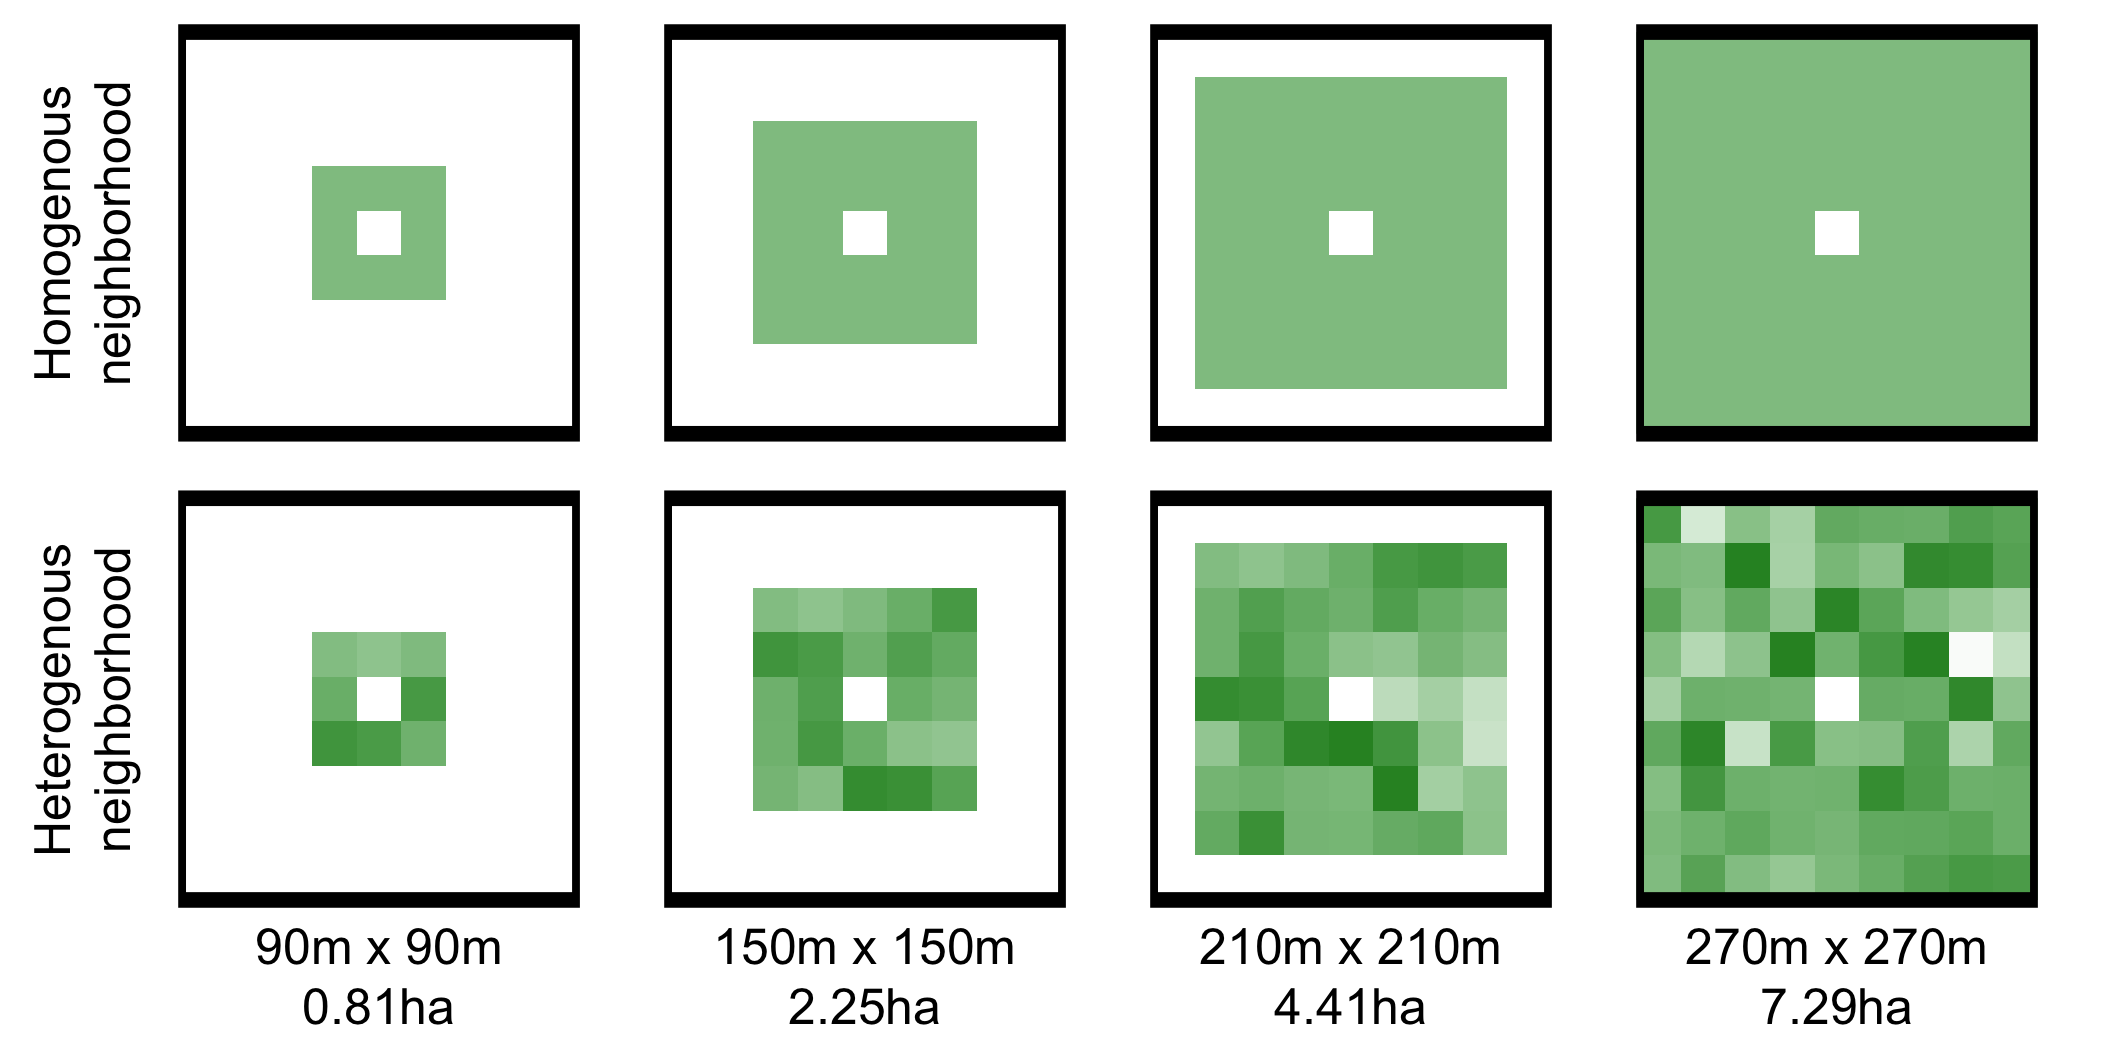
\includegraphics[width=6.00000in]{figure/chap01/heterogeneity-demo-raster.png}
\caption{Example of homogenous forest (top row) and heterogenous forest
(bottom row) with the same mean NDVI values (\textasciitilde{}0.6). Each
column represents forest structural variability measured using a
different neighborhood size. \label{fig-heterogeneity-raster}}
\end{figure}
\subsubsection{Topographic conditions}\label{topographic-conditions}

Elevation data were sourced from the Shuttle Radar Topography Mission
(Farr et al. \protect\hyperlink{ref-farr2007}{2007}), a 1-arc second
digital elevation model. Slope and aspect were extracted from the
digital elevation model. Per-pixel topographic roughness was calculated
as the standard deviation of elevation values within the same-sized
kernels as those used for variability in forest structure (90m, 150m,
210m, and 270m on a side and not including the central pixel).

We used the digital elevation model to calculate the potential annual
heat load at each pixel, which is an integrated measure of latitude,
slope, and a folding transformation of aspect about the
northeast-southwest line (McCune and Keon
(\protect\hyperlink{ref-mccune2002}{2002}) with correction in McCune
(\protect\hyperlink{ref-mccune2007}{2007}); See Supplemental Methods for
equations)

\subsubsection{Moisture conditions}\label{moisture-conditions}

The modeled 100-hour fuel moisture data were sourced from the gridMET
product, a gridded meteorological product with a daily temporal
resolution and a 4km x 4km spatial resolution (Abatzoglou
\protect\hyperlink{ref-abatzoglou2013}{2013}). We calculated 100-hour
fuel moisture as the median 100-hour fuel moisture for the 3 days prior
to the fire. The 100-hour fuel moisture is a correlate of the regional
temperature and moisture which integrates the relative humidity, the
length of day, and the amount of precipitation in the previous 24 hours.
Thus, this measure is sensitive to multiple hot dry days across the 4km
x 4km spatial extent of each grid cell, but not to diurnal variation in
relative humidity nor to extreme weather events during a fire.

\subsubsection{Remote samples}\label{remote-samples}

Approximately 100 random points were selected within each FRAP fire
perimeter in areas designated as yellow pine/mixed-conifer forest and
the values of wildfire severity as well as the values of each covariate
were extracted at those points using nearest neighbor interpolation.
Using the calibration equation described in Equation 1.1 for the best
configuration of the remote severity metric, we removed sampled points
corresponding to ``unburned'' area prior to analysis (i.e., below an RBR
threshold of 0.045). The random sampling amounted to 54109 total samples
across 972 fires.

\subsection{Modeling the effect of forest variability on
severity}\label{modeling-the-effect-of-forest-variability-on-severity}

We used the Relative Burn Ratio (RBR) calculated using bicubic
interpolation within a 48-day window to derive our response variable for
analyses of forest structural variability, as it showed the best
correspondence to field severity data measured as average
R\textsuperscript{2} in the 5-fold cross validation. Using the
non-linear relationship between RBR and CBI from the best performing
calibration model, we calculated the threshold RBR corresponding to
``high-severity'' signifying complete or near-complete overstory
mortality (RBR value of 0.282 corresponding to a CBI value of 2.25). If
the severity at a remote sample point was greater than this threshold,
the point was scored as a 1. We used a hierarchical logistic regression
model (Equation 1.2) to assess the probability of high-severity wildfire
as a linear combination of the remote metrics described above: prefire
NDVI of each pixel, standard deviation of NDVI within a neighborhood
(i.e., forest structural variability), the mean NDVI within a
neighborhood, 100-hour fuel moisture, potential annual heat load, and
topographic roughness. We included two-way interactions between the
structural variability measure and prefire NDVI, neighborhood mean NDVI,
and 100-hour fuel moisture. We include the two-way interaction between a
pixel's prefire NDVI and its neighborhood mean NDVI to account for
structural variability that may arise from differences between these
variables (see Supplemental Fig. 2). We scaled all predictor variables,
used weakly-regularizing priors, and estimated an intercept for each
individual fire with pooled variance.
\begin{enumerate}
\def\labelenumi{(\arabic{enumi})}
\setcounter{enumi}{1}
\tightlist
\item
  \(\begin{aligned} \label{eq-severity-model} severity_{i, j} &\sim Bern(\phi_{i,j}) \\ logit(\phi_{i,j}) &= \begin{aligned} & \beta_0 + \\ & \beta_{\text{nbhd\_sd\_NDVI}} * \text{nbhd\_sd\_NDVI}_i + \\ & \beta_{\text{NDVI}} * \text{NDVI}_i + \\ & \beta_{\text{nbhd\_mn\_NDVI}} * \text{nbhd\_mn\_NDVI}_i + \\ & \beta_{\text{fm100}} * \text{fm100}_i + \\ & \beta_{\text{pahl}} * \text{pahl}_i + \\ & \beta_{\text{topographic\_roughness}} * \text{topographic\_roughness}_i + \\ & \beta_{\text{nbhd\_sd\_NDVI*fm100}} * \text{nbhd\_sd\_NDVI}_i * \text{fm100}_i + \\ & \beta_{\text{nbhd\_sd\_NDVI*NDVI}} * \text{nbhd\_sd\_NDVI}_i * \text{NDVI}_i + \\ & \beta_{\text{nbhd\_sd\_NDVI*nbhd\_mn\_NDVI}} * \text{nbhd\_sd\_NDVI}_i * \text{nbhd\_mn\_NDVI}_i + \\ & \beta_{\text{nbhd\_mn\_NDVI*NDVI}} * \text{nbhd\_mn\_NDVI}_i * \text{NDVI}_i + \\ & \gamma_j \end{aligned} \\ \gamma_j &\sim \mathcal{N}(0, \sigma_{\text{fire}}) \end{aligned}\)
\end{enumerate}
\subsection{Assessing the relevant scale of forest
variability}\label{assessing-the-relevant-scale-of-forest-variability}

Each neighborhood size (90m, 150m, 210m, 270m on a side) was substituted
in turn for the neighborhood standard deviation of NDVI, neighborhood
mean NDVI, and terrain ruggedness covariates to generate a candidate set
of 4 models. To assess the scale at which the forest structure
variability effect manifests, we compared the 4 candidate models based
on different neighborhood sizes using leave-one-out cross validation
(LOO cross validation) (Vehtari et al.
\protect\hyperlink{ref-vehtari2017}{2017}). We inferred that the
neighborhood size window used in the best-performing model reflected the
scale at which the forest structure variability effect had the most
support.

\subsection{Statistical software}\label{statistical-software}

We used \texttt{R} for all statistical analyses (R Core Team
\protect\hyperlink{ref-rcoreteam2018}{2018}). We used the \texttt{brms}
package to fit mixed effects models in a Bayesian framework which
implements the No U-Turn Sampler (NUTS) extension to the Hamiltonian
Monte Carlo algorithm (Hoffman and Gelman
\protect\hyperlink{ref-hoffman2014}{2014}, Bürkner
\protect\hyperlink{ref-burkner2017}{2017}). We used 4 chains with 3000
samples per chain (1500 warmup samples and 1500 posterior samples) and
chain convergence was assessed for each estimated parameter by ensuring
Rhat values were less than or equal to 1.01 (Bürkner
\protect\hyperlink{ref-burkner2017}{2017}).

\subsection{Data availability}\label{data-availability}

All data and analysis code are available via the Open Science Framework
(\url{https://osf.io/27nsr/}) including a new dataset representing
wildfire severity, vegetation characteristics, and regional climate
conditions within the perimeters of 1,090 fires from the FRAP database
that burned in yellow pine/mixed-conifer forest in the Sierra Nevada,
California between 1984 and 2017.

\section{Acknowledgements}\label{acknowledgements}

We thank Connie Millar and Derek Young for valuable comments about this
work and we also thank the community of Google Earth Engine developers
for prompt and helpful insights about the platform. Funding was provided
by NSF Graduate Research Fellowship Grant \#DGE- 1321845 Amend. 3 (to
MJK).

\chapter{Differential response of a tree-killing bark beetle to forest
structure across a gradient of climatic water
deficit}\label{differential-response-of-a-tree-killing-bark-beetle-to-forest-structure-across-a-gradient-of-climatic-water-deficit}

Michael J. Koontz\textsuperscript{1,2,*}, Andrew M.
Latimer\textsuperscript{1,2}, Leif A. Mortenson\textsuperscript{3},
Christopher J. Fettig\textsuperscript{3}, Malcolm P.
North\textsuperscript{1,2,4}

\textsuperscript{1}Graduate Group in Ecology, University of California,
Davis, CA, USA\\
\textsuperscript{2}Department of Plant Sciences, University of
California, Davis, CA, USA\\
\textsuperscript{3}USDA Forest Service, Pacific Southwest Research
Station, Placerville, CA, USA\\
\textsuperscript{4}USDA Forest Service, Pacific Southwest Research
Station, Mammoth Lakes, CA, USA

\section{Abstract}\label{abstract-1}

The recent Californian hot drought of 2012 to 2015 created favorable
conditions for unprecedented ponderosa pine mortality in the driest,
densest portions of the Sierra Nevada mountain range, largely caused by
the western pine beetle (\emph{Dendroctonus brevicomis}). Climate
conditions related to tree water stress as well as forest structure can
influence the severity of forest insect disturbance, but it remains
challenging to consider how these variables may interact to produce
patterns of tree mortality. Previous studies have shown an interaction
between climate conditions and forest density in their effect on tree
mortality, but density is a coarse gauge of forest structure that can
affect western pine beetle behavior in a number of ways. Measuring
broad-scale climate conditions simultaneously with complex forest
structure-- including tree species, tree size, and local density-- will
refine our understanding of how these variables interact, but is
generally expensive and/or labor-intensive. We overcame these hurdles by
using a small, unhumanned aerial system (hereafter `drone') to conduct
aerial surveys over an established network of 32 forest plots along a
350km and 1000m elevation gradient in western slope Sierra yellow
pine/mixed-conifer forests. Using Structure from Motion (SfM) processing
on over 450,000 images and field measurements from the coincident ground
plots, we determined tree size, location, and species for individual
trees over 9 square kilometers of forest that experienced ponderosa pine
mortality as a result of western pine beetle activity. We modeled the
probability of ponderosa pine mortality as a linear combination of
forest structure variables and site-level climatic water deficit, and
used a Gaussian process to estimate the spatial covariance in the
response.

We found that greater host density strongly increased the probability of
host mortality, and greater host size generally decreased the
probability of host mortality. There was also a strong three-way
interaction between host density, host size, and climatic water deficit
such that host density and host size tended to synergistically increase
the probability of host mortality at hot/dry sites, but denser, smaller
trees tended to drive mortality in cool/wet sites.

Our results demonstrate a variable response of the western pine beetle
to complex forest structure across an environmental gradient during the
same hot drought, which may indicate forest sites were in different
stages of disturbance (from ``endemic'' to ``outbreak'') depending on
their regional climate. Management interventions that reduce stem
density may decrease the severity of western pine beetle disturbance in
the future, and our results suggest that focusing these treatments on
areas that are most likely to exceed feedback thresholds (i.e., hot/dry
sites with many available hosts) will have the best chance of increasing
the survivorship probability of larger trees.

\section{Introduction}\label{introduction-1}

Aggressive bark beetles dealt the final blow to many of the nearly 150
million trees killed in the California hot drought of 2012 to 2015 and
its aftermath (USDAFS \protect\hyperlink{ref-usdafs2019}{2019}). A
harbinger of climate change effects to come, record high temperatures
exacerbated the drought (Griffin and Anchukaitis
\protect\hyperlink{ref-griffin2014}{2014}), which increased water stress
on trees (Asner et al. \protect\hyperlink{ref-asner2016}{2016}), making
them more susceptible to attacking bark beetles (Fettig
\protect\hyperlink{ref-fettig2012b}{2012}, Kolb et al.
\protect\hyperlink{ref-kolb2016}{2016}). A century of fire suppression
policy has enabled forests to grow into dense stands, which also makes
them more vulnerable to bark beetle attack (Fettig
\protect\hyperlink{ref-fettig2012b}{2012}). This combination of
environmental conditions and forest structural characteristics led to
tree mortality events of unprecedented size in the driest, densest
forests across the state (Young et al.
\protect\hyperlink{ref-young2017}{2017}). The mechanisms underlying the
link between tree susceptibility to insect attack and hot, dry
conditions are often directly attributed to tree physiology (Bentz et
al. \protect\hyperlink{ref-bentz2010}{2010}), while the link to forest
density is multifaceted (Fettig
\protect\hyperlink{ref-fettig2012b}{2012}). Because forest density is a
coarse metric of the complex forest structure to which bark beetles
respond (Raffa et al. \protect\hyperlink{ref-raffa2008}{2008}), our
understanding of the connection between forest density and insect
disturbance severity could be enhanced with more finely-resolved
measures of forest structure, such as tree size, tree species, and local
density within a forest stand (Stephenson et al.
\protect\hyperlink{ref-stephenson2019}{2019}, Fettig et al.
\protect\hyperlink{ref-fettig2019}{2019}). Further, the interaction
between local-scale complex forest structure and broad-scale
environmental conditions as they affect forest insect disturbance
remains underexplored (Seidl et al.
\protect\hyperlink{ref-seidl2016a}{2016}, Stephenson et al.
\protect\hyperlink{ref-stephenson2019}{2019}, Fettig et al.
\protect\hyperlink{ref-fettig2019}{2019}).

The yellow pine/mixed-conifer forests in California's Sierra Nevada
region are characterized by regular bark beetle disturbances, primarily
by the western pine beetle (\emph{Dentrodctonus brevicomis}) and its
main host in the system, ponderosa pine (\emph{Pinus ponderosa}) (Fettig
et al. \protect\hyperlink{ref-fettig2019}{2019}). The western pine
beetle is a ``primary'' or ``aggressive'' bark beetle, with reproductive
success contingent upon enough beetles ``mass attacking'' the host tree,
overwhelming its defenses, and causing mortality (Raffa and Berryman
\protect\hyperlink{ref-raffa1983}{1983}, Fettig et al.
\protect\hyperlink{ref-fettig2019}{2019}). This Allee effect creates a
strong coupling between beetle host selection behavior and host tree
susceptibility to attack (Raffa and Berryman
\protect\hyperlink{ref-raffa1983}{1983}, Logan et al.
\protect\hyperlink{ref-logan1998}{1998}). Under normal conditions,
weakened trees are the most susceptible to attack and will be the main
targets of aggressive bark beetles like the western pine beetle (Bentz
et al. \protect\hyperlink{ref-bentz2010}{2010}, Raffa et al.
\protect\hyperlink{ref-raffa2015}{2015}). A key defense mechanism of
trees to bark beetle attack is to flood beetle bore holes with resin,
which physically expels beetles and may interrupt beetle communication
(Raffa et al. \protect\hyperlink{ref-raffa2015}{2015}). Under severe
water stress, trees no longer have the resources available to mount this
defense (Kolb et al. \protect\hyperlink{ref-kolb2016}{2016}) and thus
prolonged drought can often trigger increased bark beetle-induced tree
mortality as average tree vigor declines (Bentz et al.
\protect\hyperlink{ref-bentz2010}{2010}). As local beetle density
increases due to successful reproduction on spatially-aggregated
weakened trees, as might occur in a prolonged drought, mass attacks
become capable of overwhelming any tree's defenses and even healthy
trees become susceptible (Bentz et al.
\protect\hyperlink{ref-bentz2010}{2010}, Raffa et al.
\protect\hyperlink{ref-raffa2015}{2015}). Thus, water stress can be a
key determinant of whether individual trees are susceptible to bark
beetle attack under many conditions, and this environmental condition
may interact with other forest features, such as tree size, to drive
susceptibility under extreme conditions (Bentz et al.
\protect\hyperlink{ref-bentz2010}{2010}, Stephenson et al.
\protect\hyperlink{ref-stephenson2019}{2019}).

Forest structure-- often characterized as the spatial distribution,
size, and species composition of trees-- also strongly influences
western pine beetle activity. For instance, high-density forests are
more prone to bark beetle attacks, and several mechanism likely underlie
this phenomenon (Fettig \protect\hyperlink{ref-fettig2012b}{2012}). A
high-density forest may experience greater bark beetle-induced tree
mortality for several reasons including: a) host availability is high
and shorter dispersal distances facilitate successful colonization of
those hosts (Miller and Keen \protect\hyperlink{ref-miller1960}{1960},
Berryman \protect\hyperlink{ref-berryman1982}{1982}, Fettig et al.
\protect\hyperlink{ref-fettig2007}{2007}); b) high host availability
reduces the chance of individual beetles wasting their limited resources
flying to and landing on a non-host tree (Moeck et al.
\protect\hyperlink{ref-moeck1981}{1981}, Evenden et al.
\protect\hyperlink{ref-evenden2014}{2014}); c) crowded trees experience
greater competition for water resources and thus average tree resistance
is lower (Hayes et al. \protect\hyperlink{ref-hayes2009}{2009}); or d)
smaller gaps between trees protect pheromone plumes from dissipation by
the wind and thus enhance intraspecific beetle communication (Thistle et
al. \protect\hyperlink{ref-thistle2004}{2004}). Additionally, tree size
affects bark beetle host selection behavior as smaller trees tend to
have less capacity for resisting attack, but larger trees represent a
more desirable target because their thicker phloem provides greater
nutritional value (Chubaty et al.
\protect\hyperlink{ref-chubaty2009}{2009}, Graf et al.
\protect\hyperlink{ref-graf2012}{2012}). Tree density thus paints a
fundamentally limited picture of the mechanism by which forest structure
affects bark beetle disturbance, but \emph{complex} forest structure--
with explicit recognition of tree size, species composition (e.g., host
versus non-host composition), and local tree density-- should more
appropriately capture the ecological processes underlying insect-induced
tree mortality. Additionally, considering the effects of complex forest
structure simultaneously to the effects of environmental conditions may
help refine our understanding of observed patterns of tree mortality in
the recent California hot drought.

The vast spatial extent of tree mortality in the 2012 to 2015 California
hot drought (USDAFS \protect\hyperlink{ref-usdafs2019}{2019}) challenges
our ability to simultaneously consider how broad-scale environmental
conditions may interact with local, complex forest structure to affect
the dynamic between bark beetle host selection and host tree
susceptibility to attack (Anderegg et al.
\protect\hyperlink{ref-anderegg2015a}{2015}, Stephenson et al.
\protect\hyperlink{ref-stephenson2019}{2019}). Measuring complex forest
structure generally requires expensive instrumentation (Kane et al.
\protect\hyperlink{ref-kane2014}{2014}, Asner et al.
\protect\hyperlink{ref-asner2016}{2016}) or labor-intensive field
surveys (Larson and Churchill \protect\hyperlink{ref-larson2012}{2012},
Stephenson et al. \protect\hyperlink{ref-stephenson2019}{2019}), which
constrains survey extent and frequency. Small, unhumanned aerial systems
(sUAS) enable relatively fast and cheap remote imaging over dozens of
hectares of forest, which can be used to measure complex forest
structure at the individual tree scale (Morris et al.
\protect\hyperlink{ref-morris2017}{2017}, Shiklomanov et al.
\protect\hyperlink{ref-shiklomanov2019}{2019}). Distributing such
surveys across an environmental gradient is a viable approach to
overcoming the data acquisition challenge inherent in investigating
phenomena with both a strong local- and a strong broad-scale component.

We used ultra-high resolution, drone-derived remote sensing data over a
network of 32 sites in Sierra Nevada yellow pine/mixed-conifer forests
spanning 1000m of elevation and 350km of latitude and covering a total
of 9 square kilometers to ask how broad-scale environmental conditions
interacted with local, complex forest structure to affect the
probability of tree mortality during the cumulative tree mortality event
of 2012 to 2018. We asked:
\begin{enumerate}
\def\labelenumi{\arabic{enumi}.}
\item
  How does host tree density and average host tree size affect the
  severity of western pine beetle disturbance?
\item
  How does tree density of all species (hereafter ``overall density'')
  and average tree size of all species (hereafter ``overall size'')
  affect the severity of western pine beetle disturbance?
\item
  How does environmentally-driven tree moisture stress affect the
  severity of western pine beetle disturbance?
\item
  Do the effects of forest structure and environmental condition on
  western pine beetle disturbance interact?
\end{enumerate}
\section{Methods}\label{methods}

\subsection{Study system}\label{study-system-1}
\begin{figure}
\centering
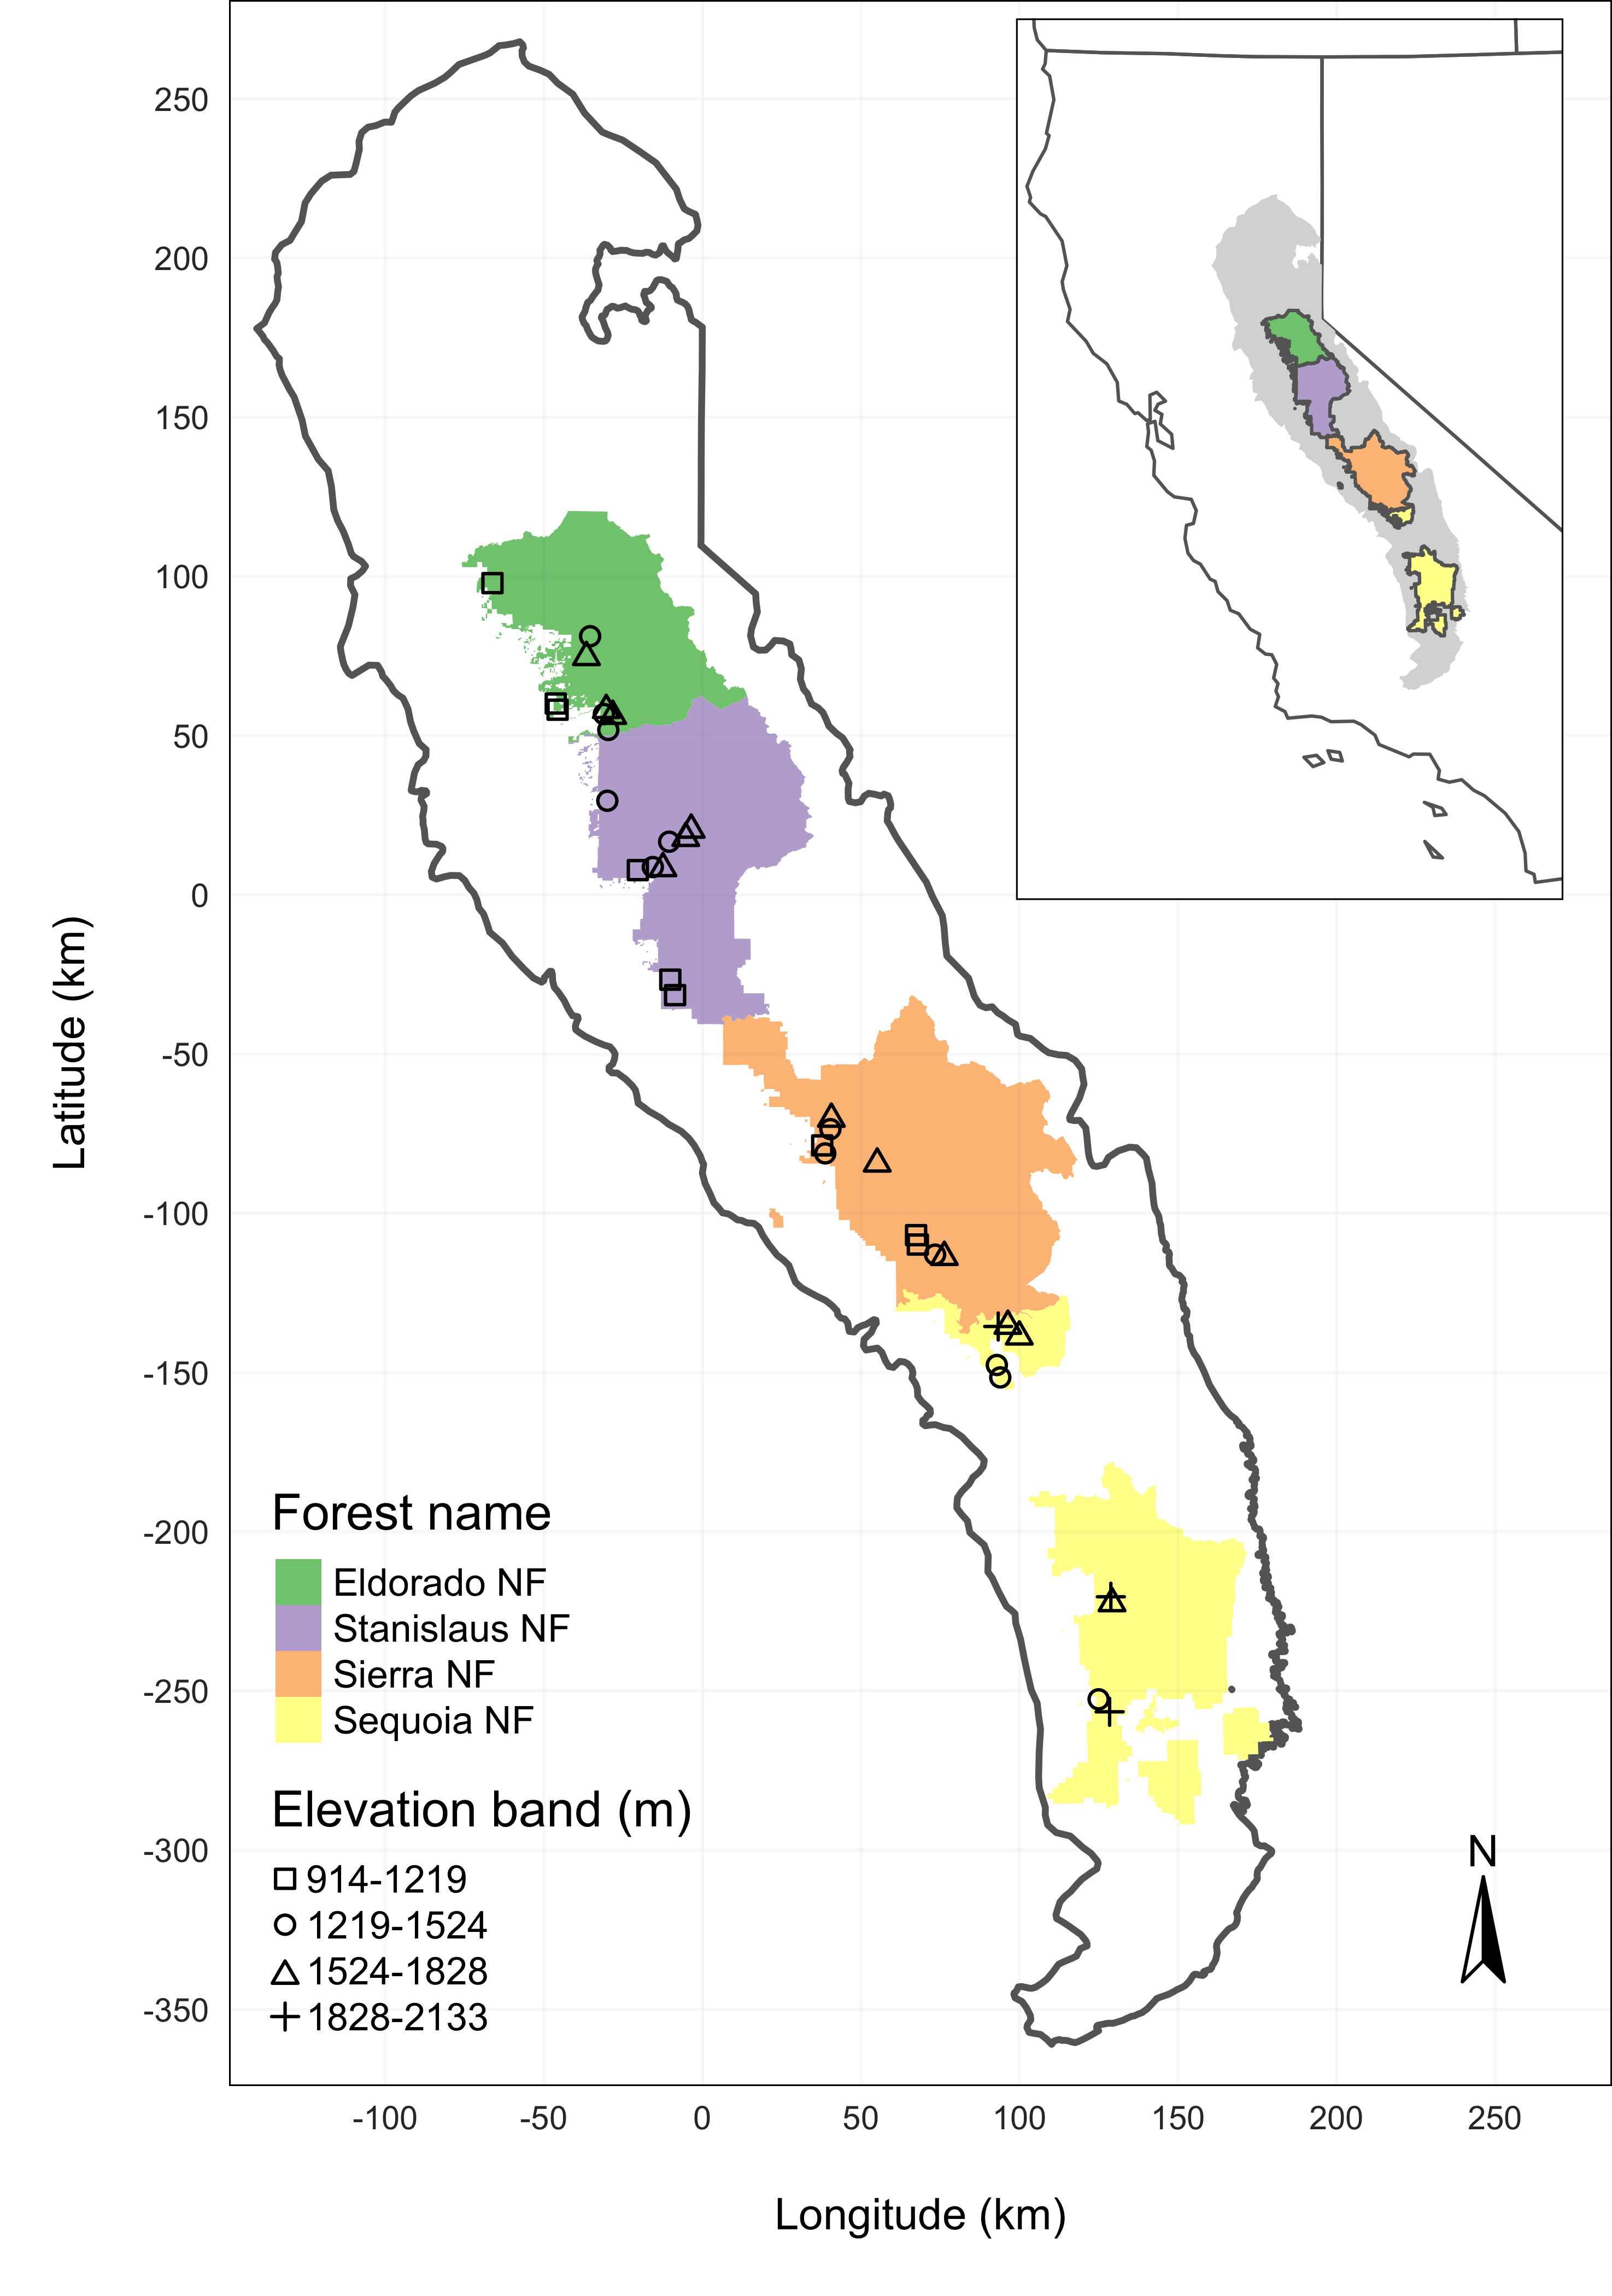
\includegraphics[height=7.00000in]{figure/chap02/study-geographic-extent-inset.png}
\caption{The network of field plots spanned a 350 km latitudinal
gradient from the Eldorado National Forest in the north to the Sequoia
National Forest in the south. Plots were stratified by three elevation
bands in each forest, with the plots in the Sequoia National Forest (the
southern-most National Forest) occupying elevation bands 305m above the
three bands in the other National Forests in order to capture a similar
community composition.}
\end{figure}
The study sites were chosen to reflect typical west-side Sierra Nevada
yellow pine/mixed-conifer forests and were dominated by ponderosa pine
trees, \emph{Pinus ponderosa} (Fettig et al.
\protect\hyperlink{ref-fettig2019}{2019}), whose primary bark beetle
predator in California is the western pine beetle (WPB),
\emph{Dendroctonus brevicomis}. The typical life cycle of WPBs consists
of pioneer beetles dispersing to a new host tree, determining the host's
susceptibility to attack, and using pheromone signals to attract other
WPBs. The attracted WPBs mass attack the tree by boring into its inner
bark, laying eggs, and dying, leaving their offspring to develop inside
the doomed tree before themselves dispersing to a new potential host
(Raffa et al. \protect\hyperlink{ref-raffa2008}{2008}). In California,
the WPB can have 2-3 generations in a single year and can often
out-compete its congener, the mountain pine beetle, \emph{Dendroctonus
ponderosa} (MPB), for the ponderosa pine host (Fettig et al.
\protect\hyperlink{ref-fettig2019}{2019}).

We built our study on 180 vegetation/forest insect monitoring plots at
36 sites established between 2016 and 2017 by Fettig et al.
(\protect\hyperlink{ref-fettig2019}{2019}) (Figure 2.1). These
established plots were located in WPB-attacked, yellow
pine/mixed-conifer forests across the Eldorado, Stanislaus, Sierra and
Sequoia National Forests and were stratified by elevation (914-1219
meters {[}3000-4000 feet{]}, 1219-1524 meters {[}4000-5000 feet{]},
1524-1828 meters {[}5000-6000 feet{]} above sea level). In the Sequoia
National Forest, the southernmost National Forest in our study, plots
were stratified with the lowest elevation band between 1219 and 1524
meters (4000-5000 feet) and extended to an upper elevation band of
1828-2133 meters (6000-7000 feet) to capture a more similar forest
community composition as at the more northern National Forests. The
sites have variable forest structure and plot locations were selected in
areas with \textgreater{}40\% ponderosa pine basal area and
\textgreater{}10\% ponderosa pine mortality. At each site, five 0.04 ha
circular plots were installed along transects with between 80 and 200m
between each plot. In the field, Fettig et al.
(\protect\hyperlink{ref-fettig2019}{2019}) mapped all stem locations
relative to the center of each plot using azimuth/distance measurements.
Tree identity to species, tree height, and diameter at breast height
(DBH) were recorded if DBH was greater than 6.35cm. Year of mortality
was estimated based on needle color and retention, if it wasn't directly
observed between site visits. A small section of bark was removed from
dead trees to confirm insect activity. During the spring and early
summer of 2018, all field plots were revisited to assess whether dead
trees had fallen (Fettig et al.
\protect\hyperlink{ref-fettig2019}{2019}).

\subsection{Instrumentation}\label{instrumentation}

Imagery was captured using a DJI Zenmuse X3 RGB camera (DJI
\protect\hyperlink{ref-dji2015}{2015}\protect\hyperlink{ref-dji2015}{a})
and a Micasense RedEdge3 5-band multispectral camera (Micasense
\protect\hyperlink{ref-micasense2015}{2015}). We mounted both of these
instruments simultaneously on a DJI Matrice 100 aircraft (DJI
\protect\hyperlink{ref-dji2015a}{2015}\protect\hyperlink{ref-dji2015a}{b})
using the DJI 3-axis stabilized gimbal for the Zenmuse X3 camera and a
Micasense angled fixed mount for the RedEdge3 camera. The gimbal and the
angled fixed mount ensured both instruments were nadir-facing during
image capture. Just prior to or after image capture at each site, we
calibrated the RedEdge3 camera by taking an image of a calibration panel
on the ground in full sun with known reflectance values for each of the
5 narrow bands (Table 2.1).
\begin{longtable}[]{@{}cccccc@{}}
\caption{Reflectance sensitivity of the Micasense Rededge3 camera. The
calibration panel value represents the reflectance of the calibration
panel for the given wavelength.}\tabularnewline
\toprule
\begin{minipage}[b]{0.10\columnwidth}\centering\strut
Band number\strut
\end{minipage} & \begin{minipage}[b]{0.23\columnwidth}\centering\strut
Band name\strut
\end{minipage} & \begin{minipage}[b]{0.14\columnwidth}\centering\strut
Center wavelength\strut
\end{minipage} & \begin{minipage}[b]{0.09\columnwidth}\centering\strut
Band width\strut
\end{minipage} & \begin{minipage}[b]{0.14\columnwidth}\centering\strut
Wavelength range\strut
\end{minipage} & \begin{minipage}[b]{0.14\columnwidth}\centering\strut
Panel reflectance\strut
\end{minipage}\tabularnewline
\midrule
\endfirsthead
\toprule
\begin{minipage}[b]{0.10\columnwidth}\centering\strut
Band number\strut
\end{minipage} & \begin{minipage}[b]{0.23\columnwidth}\centering\strut
Band name\strut
\end{minipage} & \begin{minipage}[b]{0.14\columnwidth}\centering\strut
Center wavelength\strut
\end{minipage} & \begin{minipage}[b]{0.09\columnwidth}\centering\strut
Band width\strut
\end{minipage} & \begin{minipage}[b]{0.14\columnwidth}\centering\strut
Wavelength range\strut
\end{minipage} & \begin{minipage}[b]{0.14\columnwidth}\centering\strut
Panel reflectance\strut
\end{minipage}\tabularnewline
\midrule
\endhead
\begin{minipage}[t]{0.10\columnwidth}\centering\strut
1\strut
\end{minipage} & \begin{minipage}[t]{0.23\columnwidth}\centering\strut
blue (b)\strut
\end{minipage} & \begin{minipage}[t]{0.14\columnwidth}\centering\strut
475\strut
\end{minipage} & \begin{minipage}[t]{0.09\columnwidth}\centering\strut
20\strut
\end{minipage} & \begin{minipage}[t]{0.14\columnwidth}\centering\strut
465-485\strut
\end{minipage} & \begin{minipage}[t]{0.14\columnwidth}\centering\strut
0.64\strut
\end{minipage}\tabularnewline
\begin{minipage}[t]{0.10\columnwidth}\centering\strut
2\strut
\end{minipage} & \begin{minipage}[t]{0.23\columnwidth}\centering\strut
green (g)\strut
\end{minipage} & \begin{minipage}[t]{0.14\columnwidth}\centering\strut
560\strut
\end{minipage} & \begin{minipage}[t]{0.09\columnwidth}\centering\strut
20\strut
\end{minipage} & \begin{minipage}[t]{0.14\columnwidth}\centering\strut
550-570\strut
\end{minipage} & \begin{minipage}[t]{0.14\columnwidth}\centering\strut
0.64\strut
\end{minipage}\tabularnewline
\begin{minipage}[t]{0.10\columnwidth}\centering\strut
3\strut
\end{minipage} & \begin{minipage}[t]{0.23\columnwidth}\centering\strut
red (r)\strut
\end{minipage} & \begin{minipage}[t]{0.14\columnwidth}\centering\strut
668\strut
\end{minipage} & \begin{minipage}[t]{0.09\columnwidth}\centering\strut
10\strut
\end{minipage} & \begin{minipage}[t]{0.14\columnwidth}\centering\strut
663-673\strut
\end{minipage} & \begin{minipage}[t]{0.14\columnwidth}\centering\strut
0.64\strut
\end{minipage}\tabularnewline
\begin{minipage}[t]{0.10\columnwidth}\centering\strut
4\strut
\end{minipage} & \begin{minipage}[t]{0.23\columnwidth}\centering\strut
near infrared (nir)\strut
\end{minipage} & \begin{minipage}[t]{0.14\columnwidth}\centering\strut
840\strut
\end{minipage} & \begin{minipage}[t]{0.09\columnwidth}\centering\strut
40\strut
\end{minipage} & \begin{minipage}[t]{0.14\columnwidth}\centering\strut
820-860\strut
\end{minipage} & \begin{minipage}[t]{0.14\columnwidth}\centering\strut
0.6\strut
\end{minipage}\tabularnewline
\begin{minipage}[t]{0.10\columnwidth}\centering\strut
5\strut
\end{minipage} & \begin{minipage}[t]{0.23\columnwidth}\centering\strut
red edge (re)\strut
\end{minipage} & \begin{minipage}[t]{0.14\columnwidth}\centering\strut
717\strut
\end{minipage} & \begin{minipage}[t]{0.09\columnwidth}\centering\strut
10\strut
\end{minipage} & \begin{minipage}[t]{0.14\columnwidth}\centering\strut
712-722\strut
\end{minipage} & \begin{minipage}[t]{0.14\columnwidth}\centering\strut
0.63\strut
\end{minipage}\tabularnewline
\bottomrule
\end{longtable}
\subsection{Flight protocol}\label{flight-protocol}

Image capture was conducted as close to solar noon as possible to
minimize shadow effects (varying primarily due to site accessibility;
always within 4 hours, usually within 2 hours). Prior to the aerial
survey, two strips of bright orange drop cloth (\textasciitilde{}100cm x
15cm) were positioned as an ``X'' over the permanent monuments marking
the center of the 5 field plots from Fettig et al.
(\protect\hyperlink{ref-fettig2019}{2019}).

For each of the 36 sites (containing 5 plots each), we captured imagery
over the surrounding \textasciitilde{}40 hectares of forested area using
north-south aerial transects. For three sites, we surveyed less
surrounding area in order to maintain visual and radio communication
with the aircraft during flight which can be obstructed by rolling
terrain or non-centrally available takeoff locations.

We preprogrammed aerial transects using Map Pilot for DJI on iOS flight
software (hereafter Map Pilot) (DronesMadeEasy
\protect\hyperlink{ref-dronesmadeeasy2018}{2018}). Using the Map Pilot
software, we included an altitude adjustment along each aerial transect
using a 1-arc-second digital elevation model (Farr et al.
\protect\hyperlink{ref-farr2007}{2007}) such that the aircraft's
altitude remained approximately constant at 120 meters above ground
level in order to maintain consistent ground sampling distance
(centimeters on the ground per pixel) in the imagery. Ground sampling
distance was approximately 5 cm/px for the Zenmuse X3 RGB camera and
approximately 8 cm/px for the RedEdge3 multispectral camera. For this
analysis, we dropped 4 sites whose imagery was of insufficient quality
to process.

Structure from motion (SfM) processing requires highly overlapping
images, especially in densely vegetated areas (Frey et al.
\protect\hyperlink{ref-frey2018}{2018}). We planned transects with 90\%
forward overlap and 90\% side overlap at 100 meters below the lens.
Thus, with flights being at 120 meters above ground level, we achieved
slightly higher than 90/90\% overlap for objects under 20 meters tall
(91.6/91.6\% overlap at the ground). Overlap values were based on focal
length (3.6mm), sensor width (6.2mm), and image dimension (4000x3000
pixels) parameters of the Zenmuse X3 camera. Images were captured at a
constant rate of 1 image every 2 seconds for both cameras. A forward
overlap of 90\% at 100 meters translates to a flight speed of
approximately 6.45 m/s and a side overlap of 90\% at 100 meters
translates to transects approximately 17.2 meters apart. The RedEdge3
camera has a different focal length (5.4mm), sensor width (4.8mm), and
image dimension (1280x960 pixels), which translates to image overlap of
80.7/80.7 \% at 100m below the lens and 83.9/83.9 \% at ground level.
Approximately 1900 photos were captured over each 40 hectare survey area
for each camera.

\subsection{Structure from Motion (SfM)
processing}\label{structure-from-motion-sfm-processing}

We used structure from motion (SfM) to generate dense point clouds
(Figure 2.2), digital surface models (Figure 2.3), and orthorectified
reflectance maps (Figure 2.4) for each field site (Frey et al.
\protect\hyperlink{ref-frey2018}{2018}). We used Pix4Dmapper Cloud to
process imagery using parameters ideal for images of a densely vegetated
area taken by a multispectral camera. For 29 sites, we processed the
RedEdge3 multispectral imagery alone. For three sites, we processed the
RGB and the multispectral imagery in the same project to enhance the
point density of the resulting point cloud. All SfM projects resulted in
a single processing ``block,'' indicating that all images in the project
were optimized and processed together.
\begin{figure}
\centering
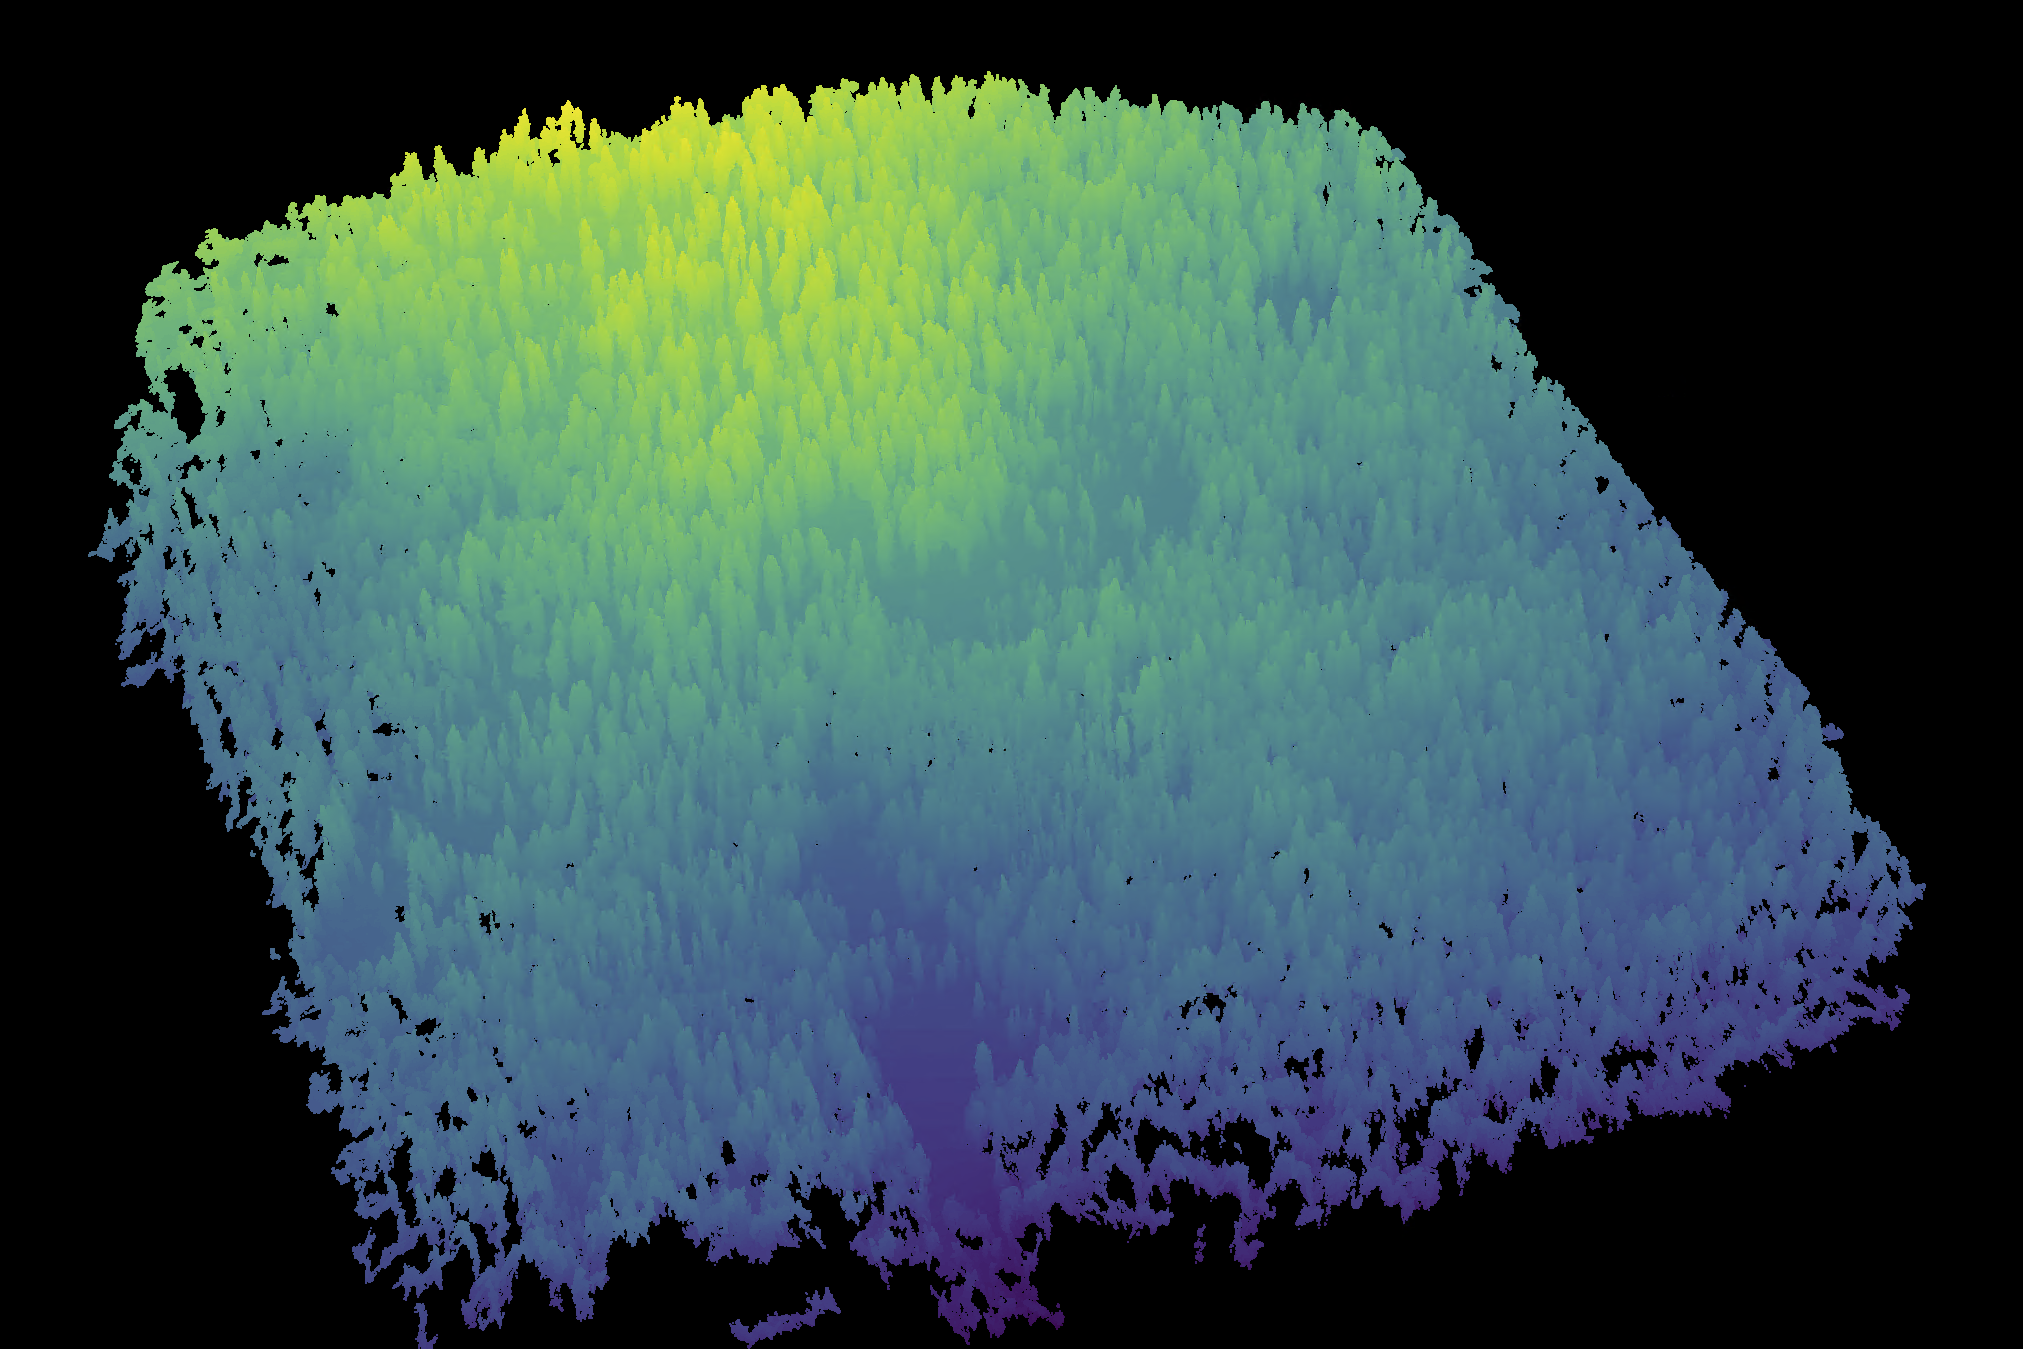
\includegraphics[width=6.00000in]{figure/chap02/eldo_3k_3_point_cloud.png}
\caption{A dense point cloud representing \textasciitilde{}40 hectares
of forest is generated using Structure from Motion (SfM) processing of
\textasciitilde{}1900 images. The dense point cloud z- position
represents the ground elevation plus the vegetation height.}
\end{figure}
\begin{figure}
\centering
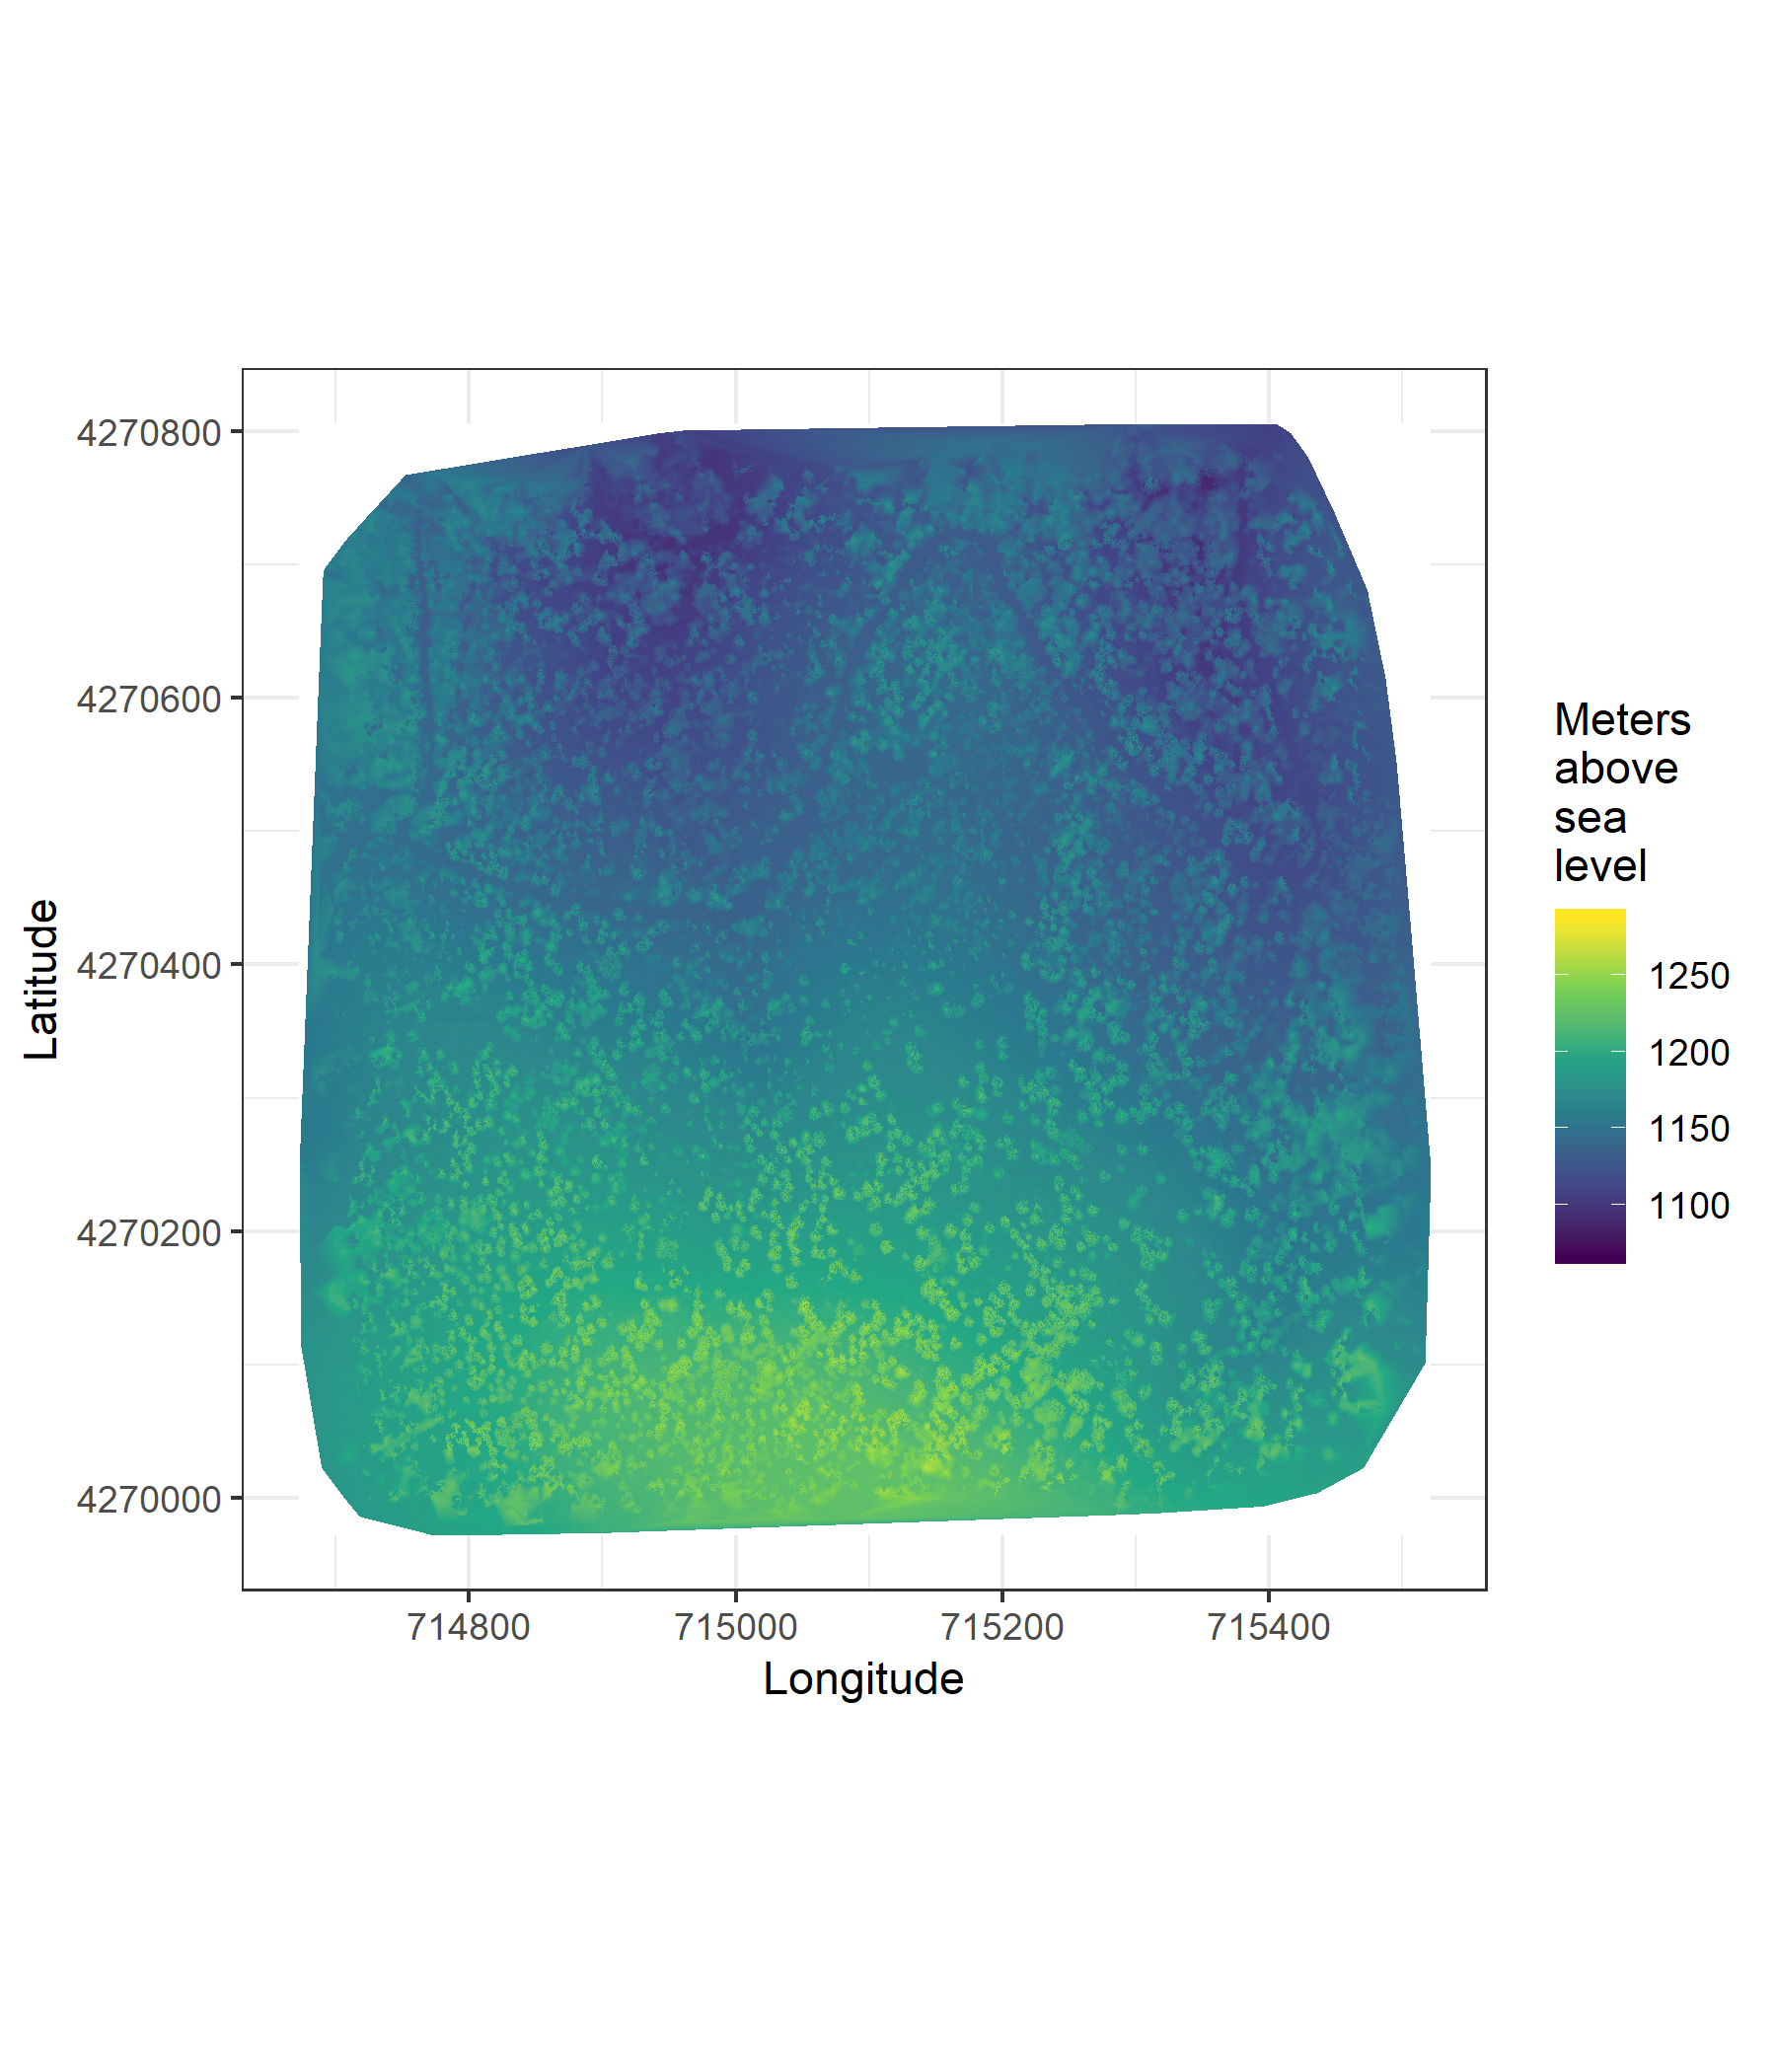
\includegraphics[width=6.00000in]{figure/chap02/eldo_3k_3_dsm.png}
\caption{The digital surface model (DSM) is a 2-dimensional
representation of the dense point cloud generated using structure from
motion (SfM) processing. The DSM represents the ground elevation plus
the vegetation height.}
\end{figure}
\begin{figure}
\centering
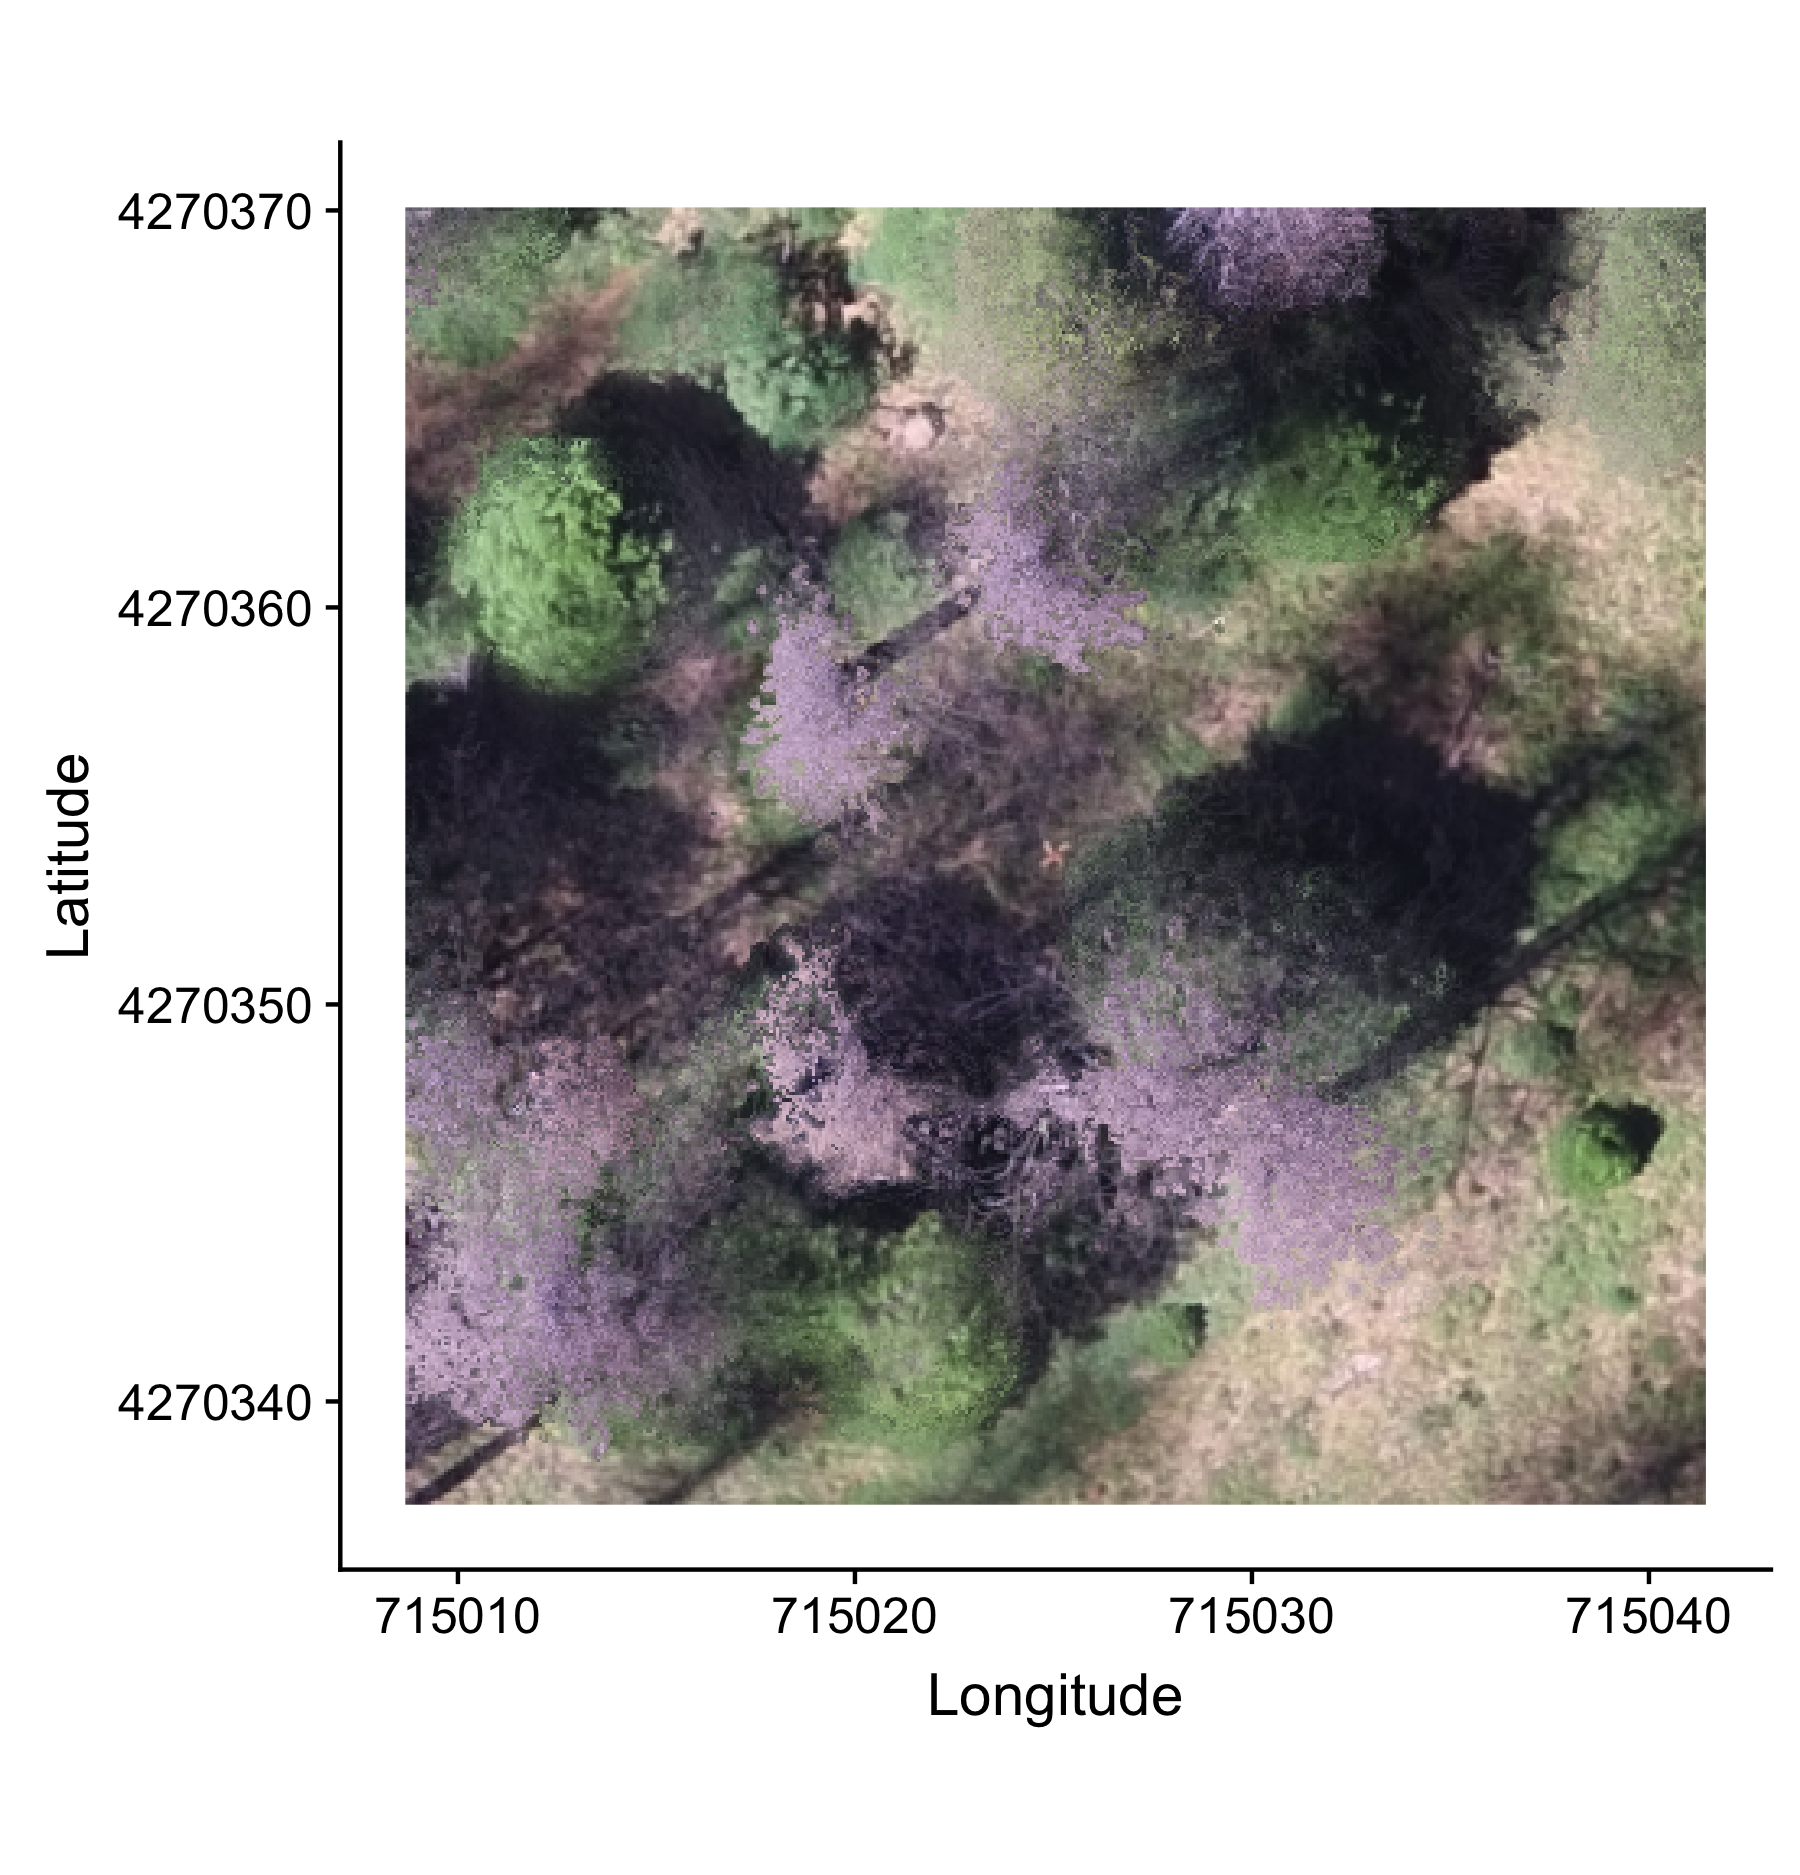
\includegraphics[width=6.00000in]{figure/chap02/eldo_3k_3_2_ortho-rgb.png}
\caption{The orthomosaic for each of the 32 sites is generated with the
Structure from Motion (SfM) processing, showing a top-down view of the
whole survey area such that distances between objects in the scene are
preserved and can be measured. Depicted is an example orthomosaic for
one of the 32 sites cropped to the extent of a single ground plot (5
ground plots per site) showing the orange X placed at exactly the plot
center prior to flight. The original orthomosaic for the whole site
represents an area approximately 1000 times as large as the area
depicted here.}
\end{figure}
\subsection{Creating canopy height
models}\label{creating-canopy-height-models}
\begin{figure}
\centering
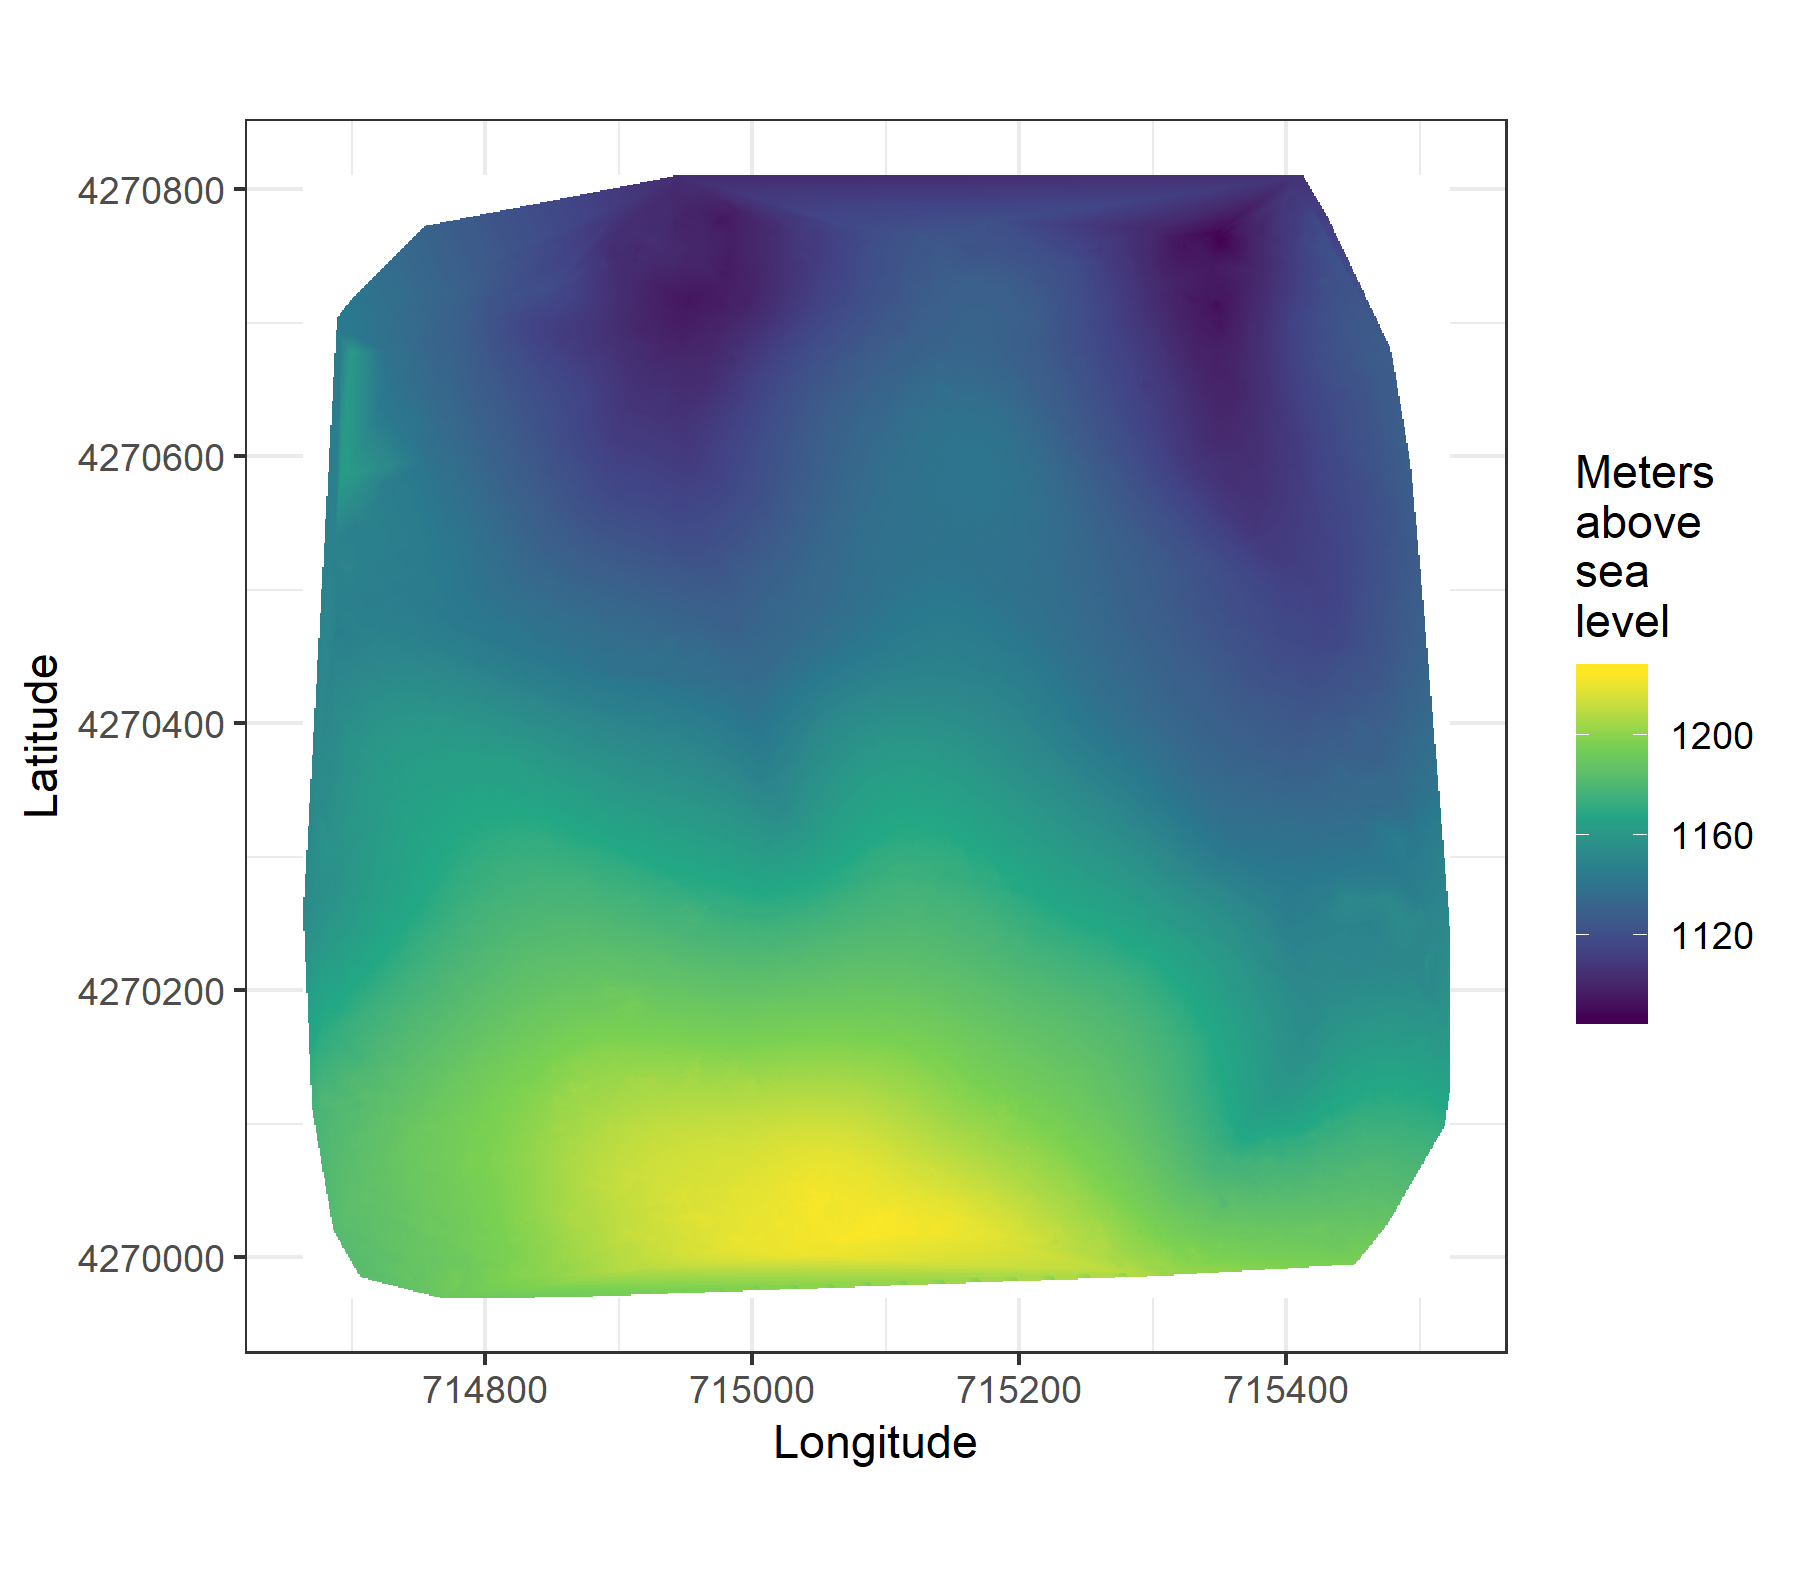
\includegraphics[width=6.00000in]{figure/chap02/eldo_3k_3_dtm.png}
\caption{The digital terrain model (DTM) is generated by processing the
dense point cloud using the cloth simulation filter algorithm (Zhang et
al. \protect\hyperlink{ref-zhang2016}{2016}), which classifies points as
`ground' or `not-ground' and then interpolates the `ground' elevation
using Delaunay triangulation for the rest of the dense point cloud
footprint. The DTM represents the ground elevation without any
vegetation.}
\end{figure}
\begin{figure}
\centering
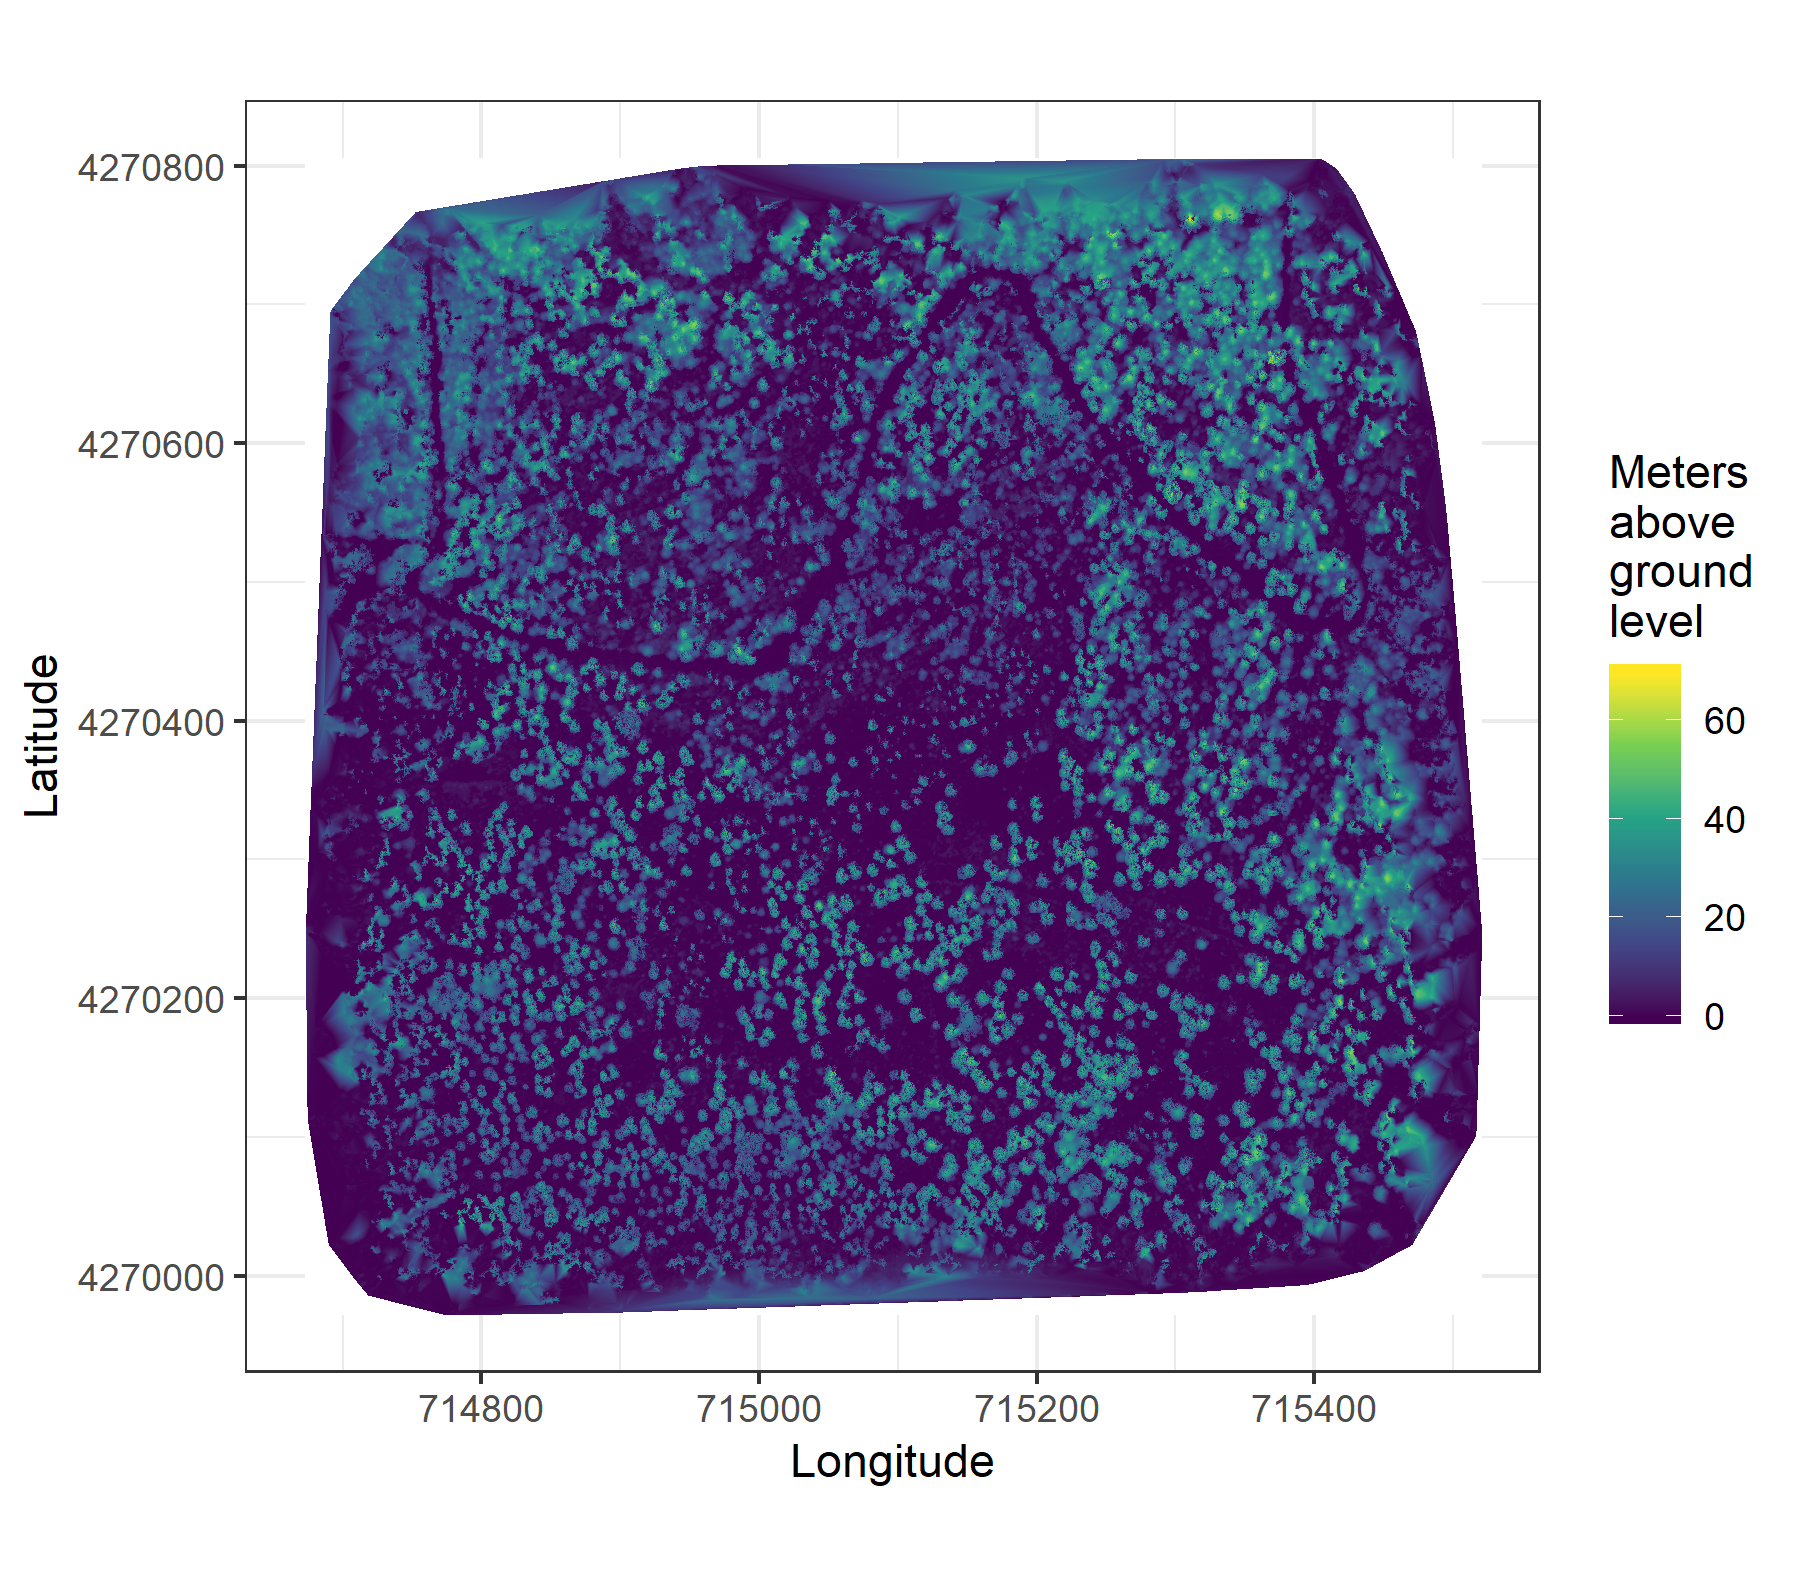
\includegraphics[width=6.00000in]{figure/chap02/eldo_3k_3_chm.png}
\caption{The canopy height model (CHM) is generated by subtracting the
digital terrain model from the digital surface model. The CHM represents
the height of all of the elevation above ground level.}
\end{figure}
We classified each survey area's dense point cloud into ``ground'' and
``non-ground'' points using a cloth simulation filter algorithm (Zhang
et al. \protect\hyperlink{ref-zhang2016}{2016}) implemented in the
\texttt{lidR} (Roussel et al. \protect\hyperlink{ref-roussel2019}{2019})
package. We rasterized the ground points using the \texttt{raster}
package (Hijmans et al. \protect\hyperlink{ref-hijmans2019}{2019}) to
create a digital terrain model (Figure 2.5) representing the ground
underneath the vegetation at 1 meter resolution. We created a canopy
height model (Figure 2.6) by subtracting the digital terrain model from
the digital surface model created in Pix4Dmapper.

\subsection{Tree detection}\label{tree-detection}

We tested a total of 7 automatic tree detection algorithms and a total
of 177 parameter sets on the canopy height model or the dense point
cloud to locate trees within each site (Table 2.2). We used 3 parameter
sets of a variable window filter using the \texttt{vwf()} function in
the \texttt{ForestTools} (Plowright
\protect\hyperlink{ref-plowright2018}{2018}\protect\hyperlink{ref-plowright2018}{b})
\texttt{R} package, including the default \texttt{winFun} parameter for
the \texttt{vwf()} function as well as the ``pines'' and ``combined''
functions from Popescu and Wynne
(\protect\hyperlink{ref-popescu2004}{2004}) as the \texttt{winFun}
parameter. We used 6 parameter sets of a local maximum filter
implemented in \texttt{lidR}. We used 131 parameter sets of the
algorithm from Li et al. (\protect\hyperlink{ref-li2012}{2012}), which
operates on the original point cloud. These parameter sets included
those from Shin et al. (\protect\hyperlink{ref-shin2018}{2018}) and
Jakubowski et al. (\protect\hyperlink{ref-jakubowski2013}{2013}). We
used 3 parameter sets of the \texttt{watershed} algorithm implemented in
\texttt{lidR}, which is a wrapper for a function in the \texttt{EBImage}
package (Pau et al. \protect\hyperlink{ref-pau2010}{2010}). We used 3
parameter sets of \texttt{ptrees} (Vega et al.
\protect\hyperlink{ref-vega2014}{2014}) implemented in \texttt{lidR}
(Roussel et al. \protect\hyperlink{ref-roussel2019}{2019}) and
\texttt{lidRplugins} (Roussel
\protect\hyperlink{ref-roussel2019a}{2019}) and which operates on the
raw point cloud, without first normalizing it to height above ground
level (i.e.. subtracting the ground elevation from the dense point
cloud). We used the default parameter set of the \texttt{multichm} (Eysn
et al. \protect\hyperlink{ref-eysn2015}{2015}) algorithm implemented in
\texttt{lidR} (Roussel et al. \protect\hyperlink{ref-roussel2019}{2019})
and \texttt{lidRplugins} (Roussel
\protect\hyperlink{ref-roussel2019a}{2019}). Finally, we used 30
parameter sets of the experimental algorithm \texttt{lmfx} (Roussel
\protect\hyperlink{ref-roussel2019a}{2019}).
\begin{longtable}[]{@{}ccc@{}}
\caption{Algorithm name, number of parameter sets tested for each
algorithm, and references.}\tabularnewline
\toprule
\begin{minipage}[b]{0.18\columnwidth}\centering\strut
Algorithm\strut
\end{minipage} & \begin{minipage}[b]{0.22\columnwidth}\centering\strut
Parameter sets tested\strut
\end{minipage} & \begin{minipage}[b]{0.34\columnwidth}\centering\strut
Reference(s)\strut
\end{minipage}\tabularnewline
\midrule
\endfirsthead
\toprule
\begin{minipage}[b]{0.18\columnwidth}\centering\strut
Algorithm\strut
\end{minipage} & \begin{minipage}[b]{0.22\columnwidth}\centering\strut
Parameter sets tested\strut
\end{minipage} & \begin{minipage}[b]{0.34\columnwidth}\centering\strut
Reference(s)\strut
\end{minipage}\tabularnewline
\midrule
\endhead
\begin{minipage}[t]{0.18\columnwidth}\centering\strut
li2012\strut
\end{minipage} & \begin{minipage}[t]{0.22\columnwidth}\centering\strut
131\strut
\end{minipage} & \begin{minipage}[t]{0.34\columnwidth}\centering\strut
Li et al. (\protect\hyperlink{ref-li2012}{2012}); Jakubowski et al.
(\protect\hyperlink{ref-jakubowski2013}{2013}); Shin et al.
(\protect\hyperlink{ref-shin2018}{2018})\strut
\end{minipage}\tabularnewline
\begin{minipage}[t]{0.18\columnwidth}\centering\strut
lmfx\strut
\end{minipage} & \begin{minipage}[t]{0.22\columnwidth}\centering\strut
30\strut
\end{minipage} & \begin{minipage}[t]{0.34\columnwidth}\centering\strut
Roussel (\protect\hyperlink{ref-roussel2019a}{2019})\strut
\end{minipage}\tabularnewline
\begin{minipage}[t]{0.18\columnwidth}\centering\strut
localMaxima\strut
\end{minipage} & \begin{minipage}[t]{0.22\columnwidth}\centering\strut
6\strut
\end{minipage} & \begin{minipage}[t]{0.34\columnwidth}\centering\strut
Roussel et al. (\protect\hyperlink{ref-roussel2019}{2019})\strut
\end{minipage}\tabularnewline
\begin{minipage}[t]{0.18\columnwidth}\centering\strut
multichm\strut
\end{minipage} & \begin{minipage}[t]{0.22\columnwidth}\centering\strut
1\strut
\end{minipage} & \begin{minipage}[t]{0.34\columnwidth}\centering\strut
Eysn et al. (\protect\hyperlink{ref-eysn2015}{2015})\strut
\end{minipage}\tabularnewline
\begin{minipage}[t]{0.18\columnwidth}\centering\strut
ptrees\strut
\end{minipage} & \begin{minipage}[t]{0.22\columnwidth}\centering\strut
3\strut
\end{minipage} & \begin{minipage}[t]{0.34\columnwidth}\centering\strut
Vega et al. (\protect\hyperlink{ref-vega2014}{2014})\strut
\end{minipage}\tabularnewline
\begin{minipage}[t]{0.18\columnwidth}\centering\strut
vwf\strut
\end{minipage} & \begin{minipage}[t]{0.22\columnwidth}\centering\strut
3\strut
\end{minipage} & \begin{minipage}[t]{0.34\columnwidth}\centering\strut
Plowright
(\protect\hyperlink{ref-plowright2018}{2018}\protect\hyperlink{ref-plowright2018}{b})\strut
\end{minipage}\tabularnewline
\begin{minipage}[t]{0.18\columnwidth}\centering\strut
watershed\strut
\end{minipage} & \begin{minipage}[t]{0.22\columnwidth}\centering\strut
3\strut
\end{minipage} & \begin{minipage}[t]{0.34\columnwidth}\centering\strut
Pau et al. (\protect\hyperlink{ref-pau2010}{2010})\strut
\end{minipage}\tabularnewline
\bottomrule
\end{longtable}
\subsection{Map ground data}\label{map-ground-data}

Each orthorectified reflectance map was inspected to locate the 5 orange
``X''s marking the center of the field plots (Figure 2.4), though some
plot centers were obscured due to dense interlocking tree crowns or
because a plot center was located directly under a single tree crown. We
were able to locate 110 out of 180 field plots and were then able to use
these plots for validation of automated tree detection algorithms. We
used the \texttt{sf} package (Pebesma et al.
\protect\hyperlink{ref-pebesma2019}{2019}) to convert
distance-from-center and azimuth measurements of each tree in the ground
plots to an x-y position on the SfM-derived reflectance map using the
x-y position of the orange X visible in the reflectance map as the
center.

\subsection{Correspondence of automatic tree detection with ground
data}\label{correspondence-of-automatic-tree-detection-with-ground-data}

We calculated 7 forest structure metrics for each field plot using the
ground data collected by Fettig et al.
(\protect\hyperlink{ref-fettig2019}{2019}): total number of trees,
number of trees greater than 15 meters, mean height of trees,
25\textsuperscript{th} percentile tree height, 75\textsuperscript{th}
percentile tree height, mean distance to nearest tree neighbor, mean
distance to 2\textsuperscript{nd} nearest neighbor.

For each tree detection algorithm and parameter set described above, we
calculated the same set of 7 structure metrics within the footprint of
the validation field plots. We calculated the Pearson's correlation and
root mean square error (RMSE) between the ground data and the aerial
data for each of the 7 structure metrics for each of the 177 automatic
tree detection algorithms/parameter sets.

For each algorithm and parameter set, we calculated its performance
relative to other algorithms as whether its Pearson's correlation was
within 5\% of the highest Pearson's correlation as well as whether its
RMSE was within 5\% of the lowest RMSE. For each algorithm/parameter
set, we summed the number of forest structure metrics for which it
reached these 5\% thresholds. For automatically detecting trees across
the whole study, we selected the algorithm/parameter set that performed
well across the most number of forest metrics (Figure 2.7).
\begin{figure}
\centering
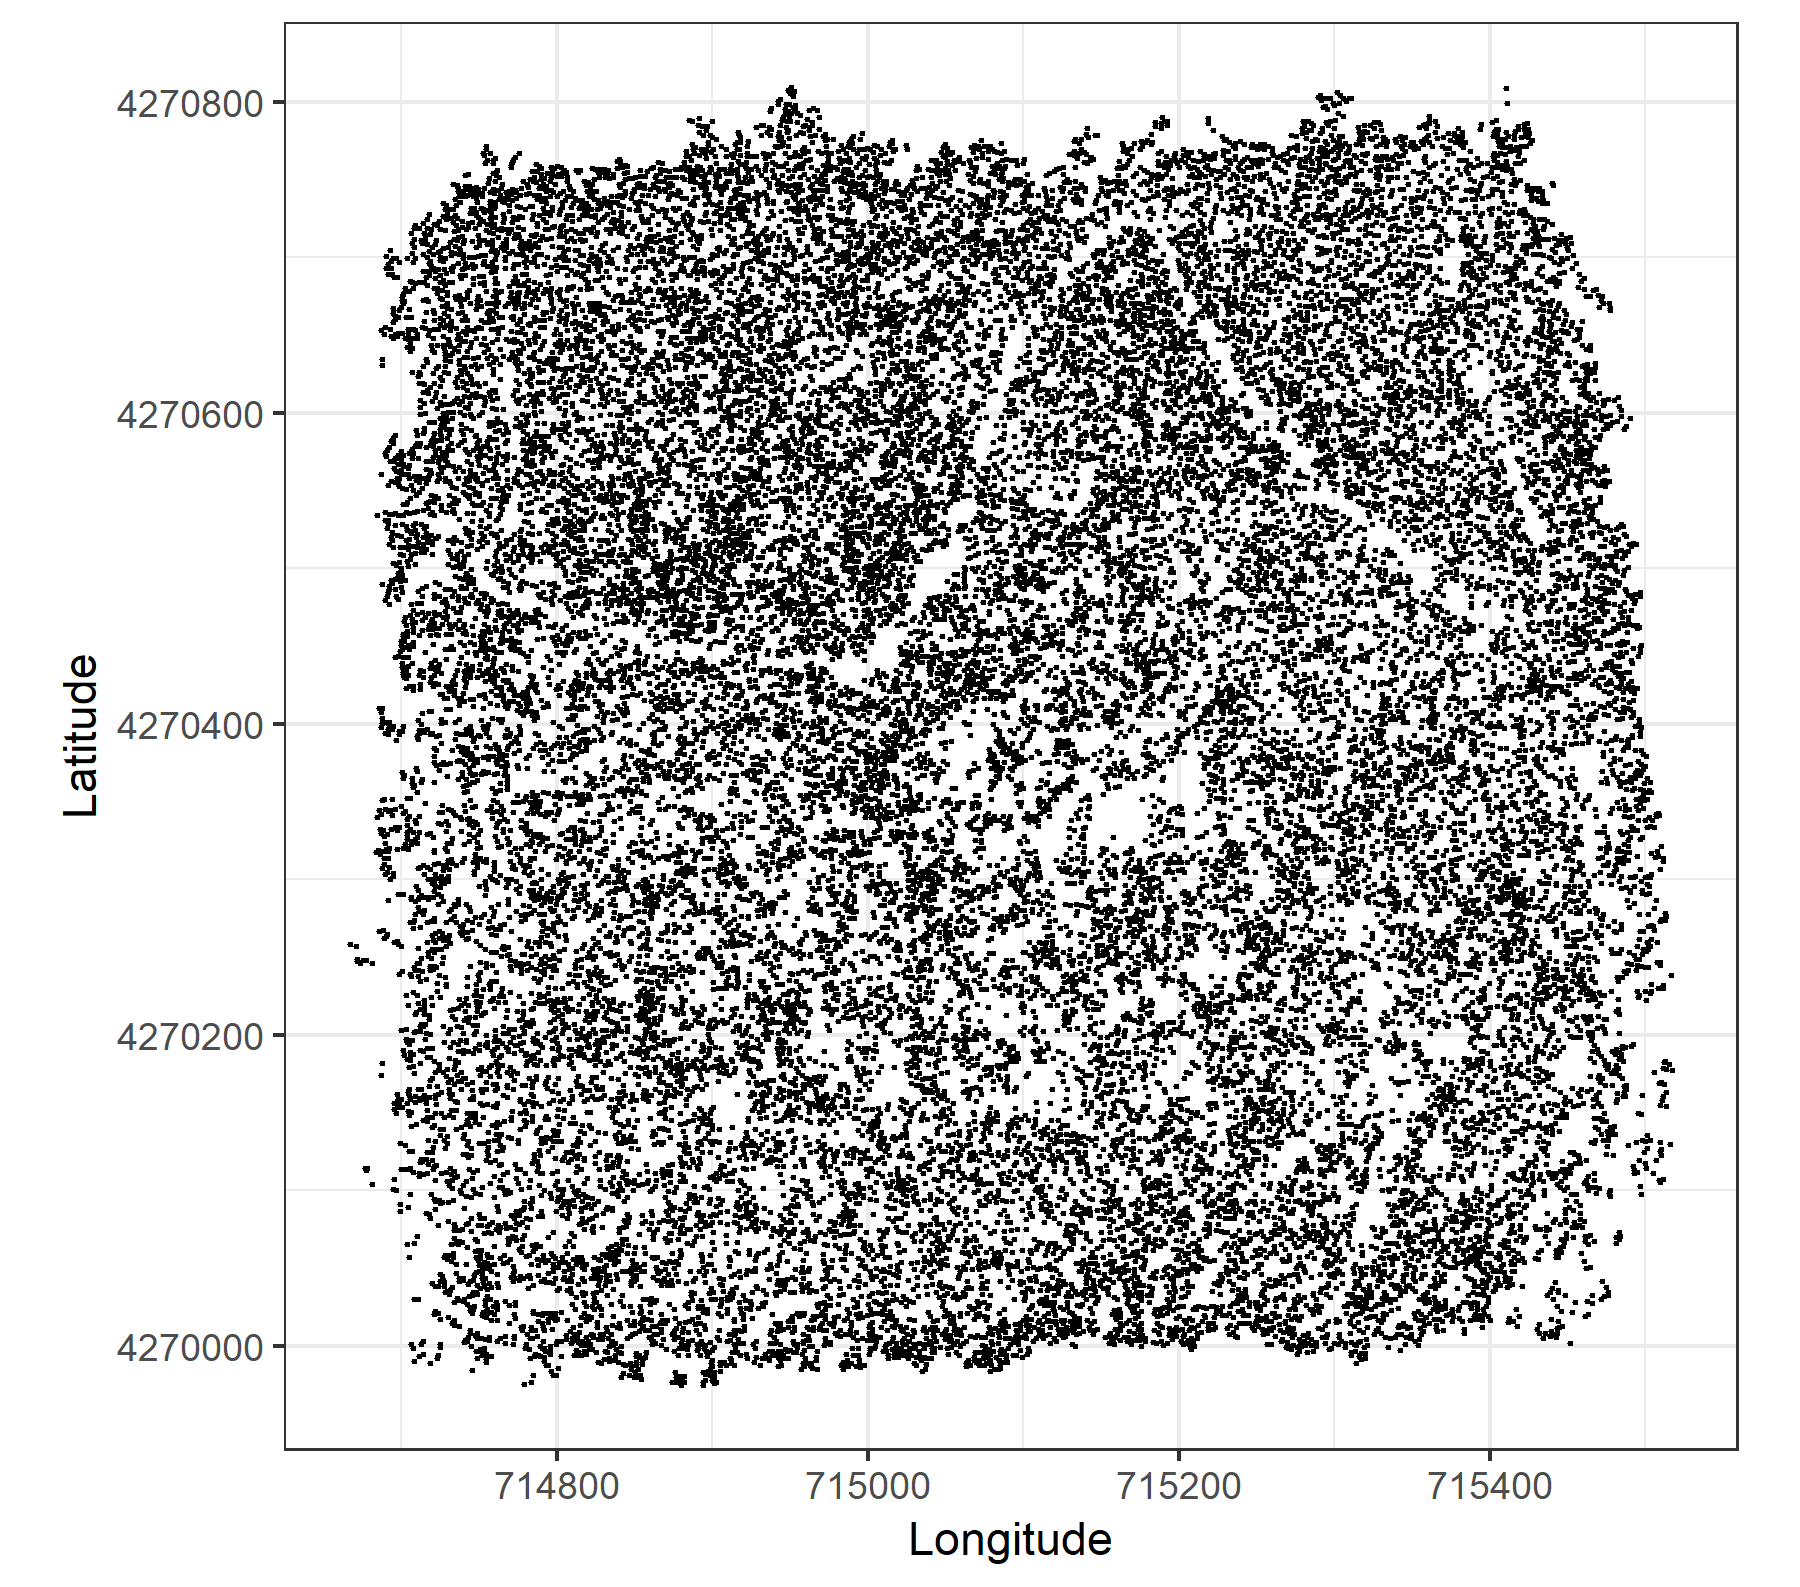
\includegraphics[width=6.00000in]{figure/chap02/eldo_3k_3_ttops.png}
\caption{Tree locations are detected using the \texttt{lmfx} (Roussel et
al. \protect\hyperlink{ref-roussel2019}{2019}) treetop detection
algorithm on the dense point cloud.}
\end{figure}
\subsection{Segmentation of crowns}\label{segmentation-of-crowns}
\begin{figure}
\centering
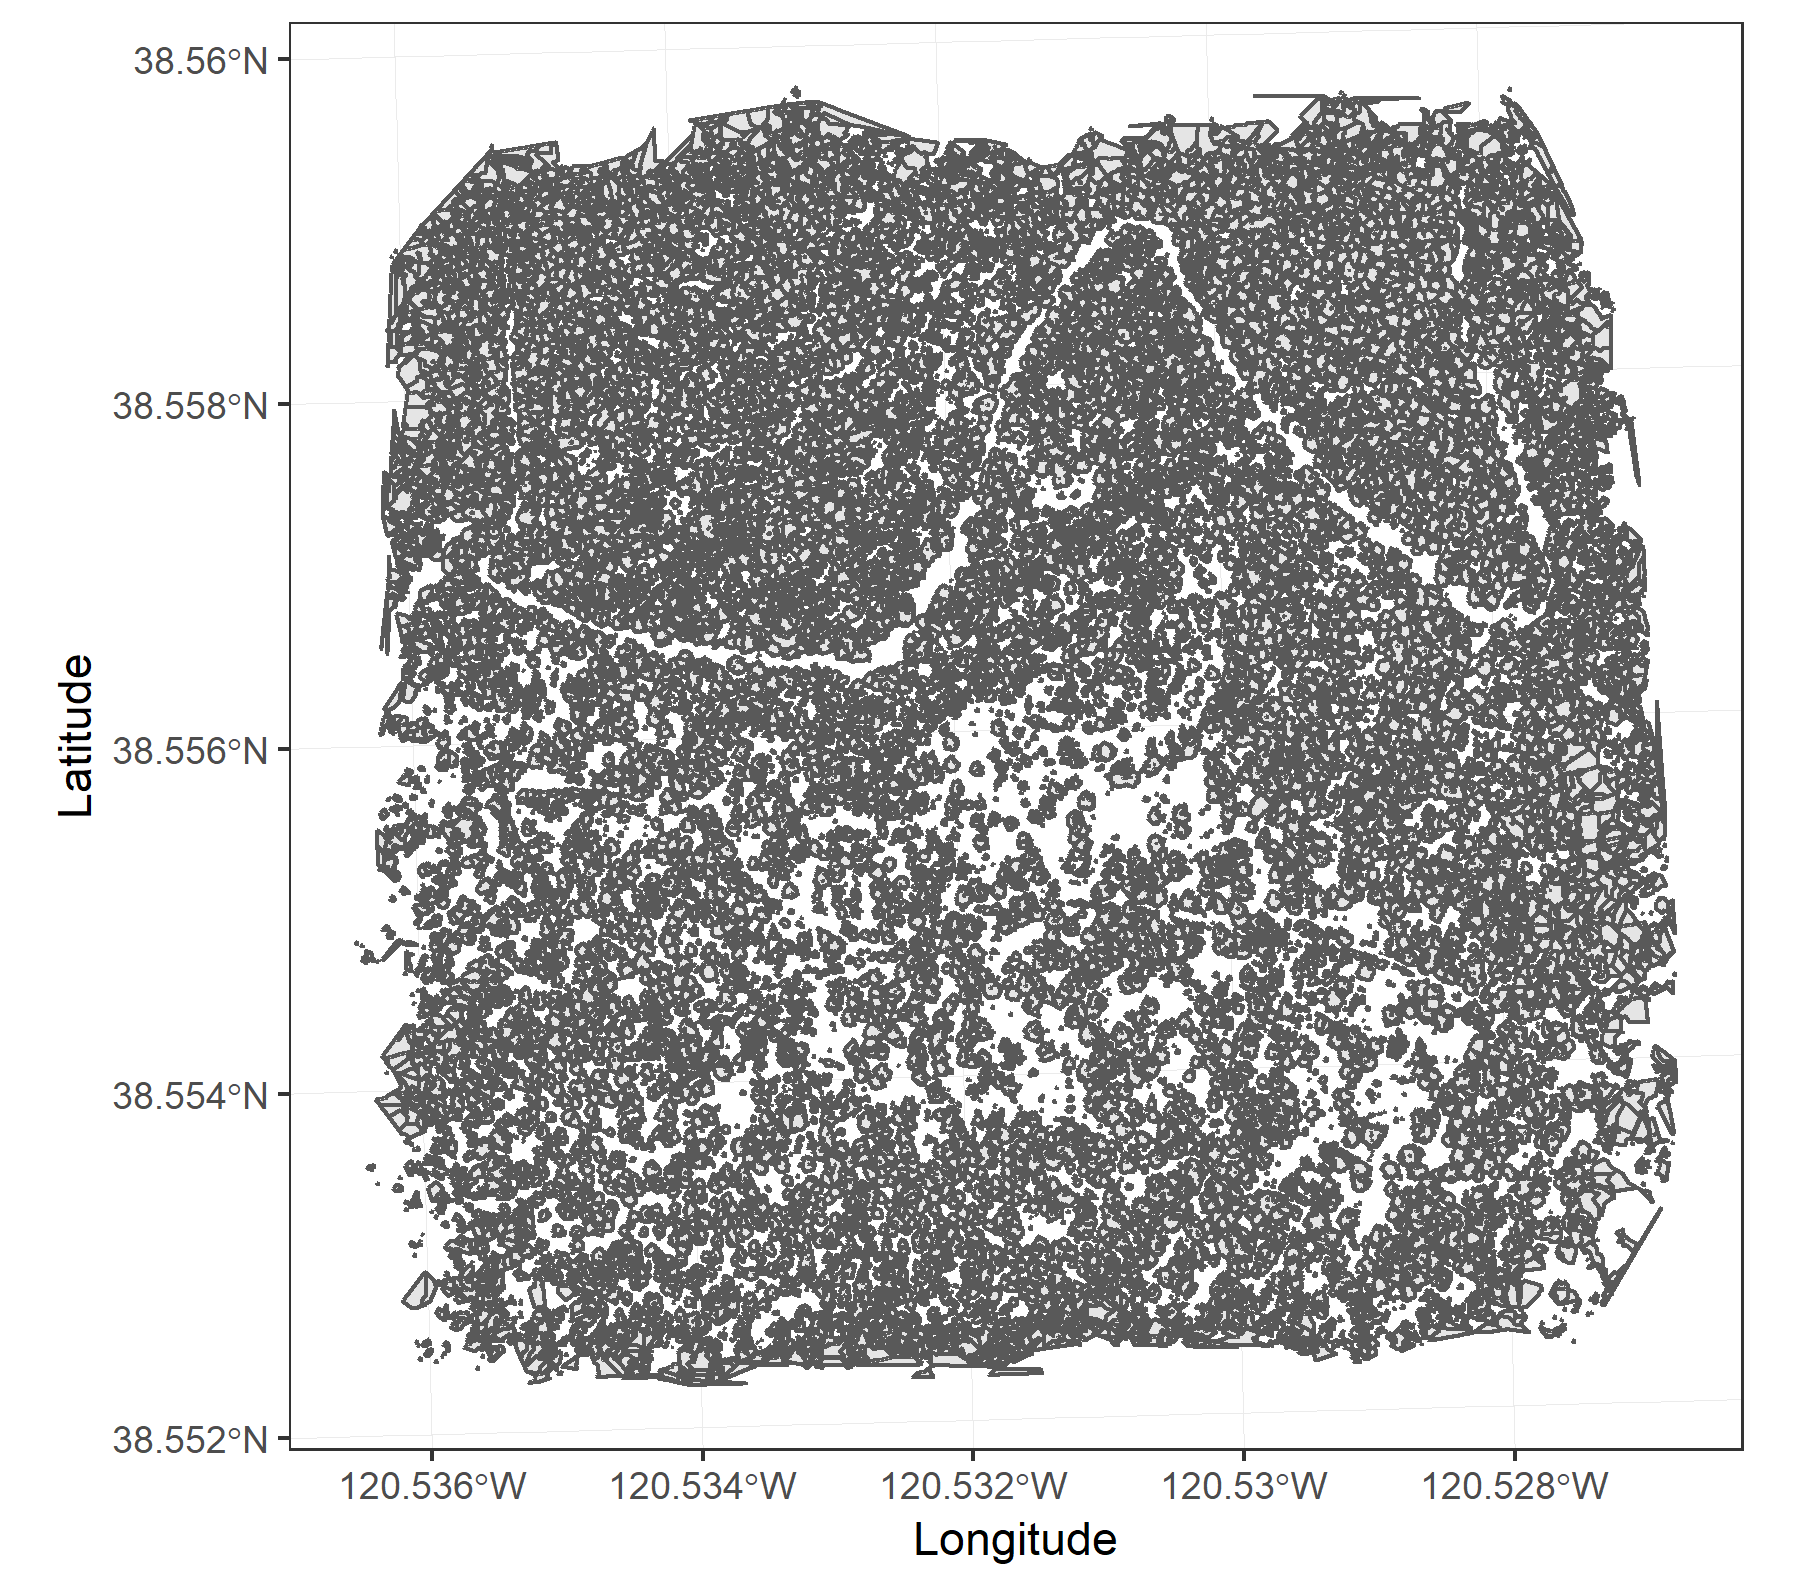
\includegraphics[width=6.00000in]{figure/chap02/eldo_3k_3_crowns.png}
\caption{Individual crowns are delineated using a marker controlled
watershed segmentation algorithm (Meyer and Beucher
\protect\hyperlink{ref-meyer1990}{1990}, Plowright
\protect\hyperlink{ref-plowright2018}{2018}\protect\hyperlink{ref-plowright2018}{b})
on the canopy height model (CHM) using the detected tree locations as a
priority map. If the algorithm failed to delineate a crown for a tree
that was identified in the tree detection step, a circular crown with a
0.5m buffer centered on point location of the detected tree was added as
a crown.}
\end{figure}
We delineated individual tree crowns with a marker controlled watershed
segmentation algorithm (Meyer and Beucher
\protect\hyperlink{ref-meyer1990}{1990}) using the detected treetops as
markers implemented in the \texttt{ForestTools} package (Plowright
\protect\hyperlink{ref-plowright2018}{2018}\protect\hyperlink{ref-plowright2018}{b}).
If the automatic segmentation algorithm failed to generate a crown
segment for a detected tree (e.g., often snags with a very small crown
footprint), a circular crown was generated with a radius of 0.5 meters.
If the segmentation generated multiple polygons for a single detected
tree, only the polygon containing the detected tree was retained (Figure
2.8). Image overlap decreases near the edges of the overall flight path,
which reduces the quality of the SfM processing in those areas. Thus, we
excluded segmented crowns within 35 meters of the edge of the survey
area. Given the narrower field of view of the RedEdge3 multispectral
camera versus the X3 RGB camera whose optical parameters were used to
define the \textasciitilde{}40 hectare survey area around each site, as
well as the 35 meter additional buffering, the survey area at each site
was approximately 30 hectares (Table 2.3).

We used the \texttt{velox} package (Hunziker
\protect\hyperlink{ref-hunziker2017}{2017}) to extract all the pixel
values from the orthorectified reflectance map for each of the 5 narrow
bands within each segmented crown polygon. Per pixel, we additionally
calculated the normalized difference vegetation index (NDVI; Rouse et
al. (\protect\hyperlink{ref-rouse1973}{1973})), the normalized
difference red edge (NDRE; Gitelson and Merzlyak
(\protect\hyperlink{ref-gitelson1994}{1994})), the red-green index (RGI;
Coops et al. (\protect\hyperlink{ref-coops2006}{2006})), the red edge
chlorophyll index (CI\textsubscript{red} \textsubscript{edge}; Clevers
and Gitelson (\protect\hyperlink{ref-clevers2013}{2013})), and the green
chlorophyll index (CI\textsubscript{green}; Clevers and Gitelson
(\protect\hyperlink{ref-clevers2013}{2013})). For each crown polygon, we
calculated the mean value for each raw and derived reflectance band (5
raw; 5 derived).

\subsection{Classification of trees}\label{classification-of-trees}
\begin{figure}
\centering
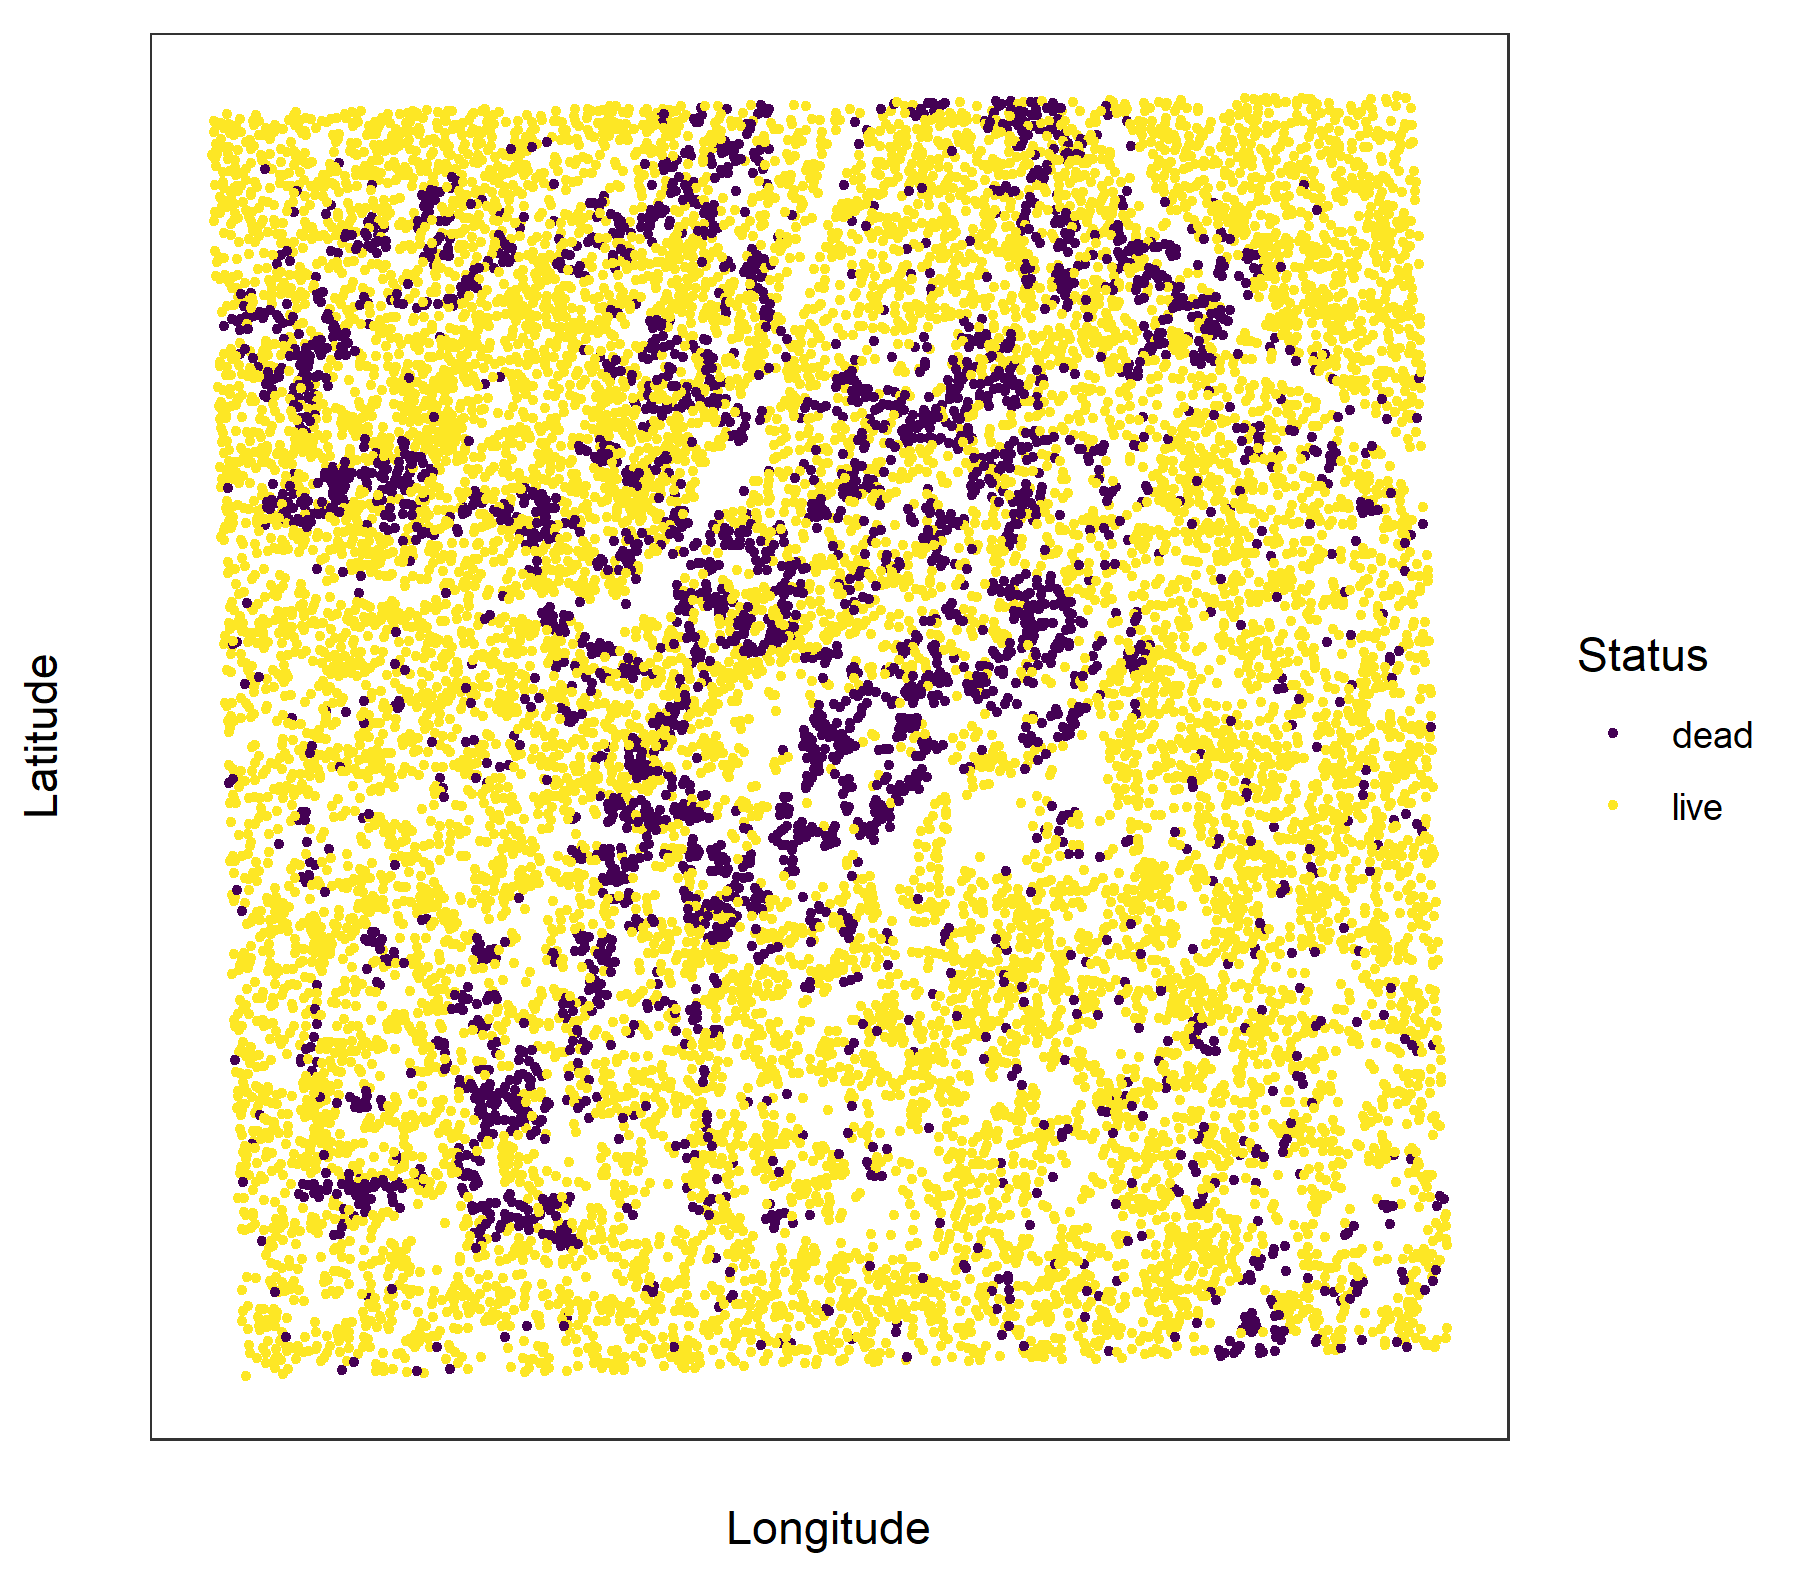
\includegraphics[width=6.00000in]{figure/chap02/eldo_3k_3_live_dead.png}
\caption{Each tree is classified as live or dead by extracting the pixel
values from the 5 narrow bands of the Rededge3 camera (and 5 derived
bands-- see methods) in the orthomosaic within each segmented tree crown
of the detected trees, taking their mean value, and using those means to
predict live/dead status with a boosted logistic regression previously
trained on a hand-classified set of segmented crowns from across the
study area.}
\end{figure}
\begin{figure}
\centering
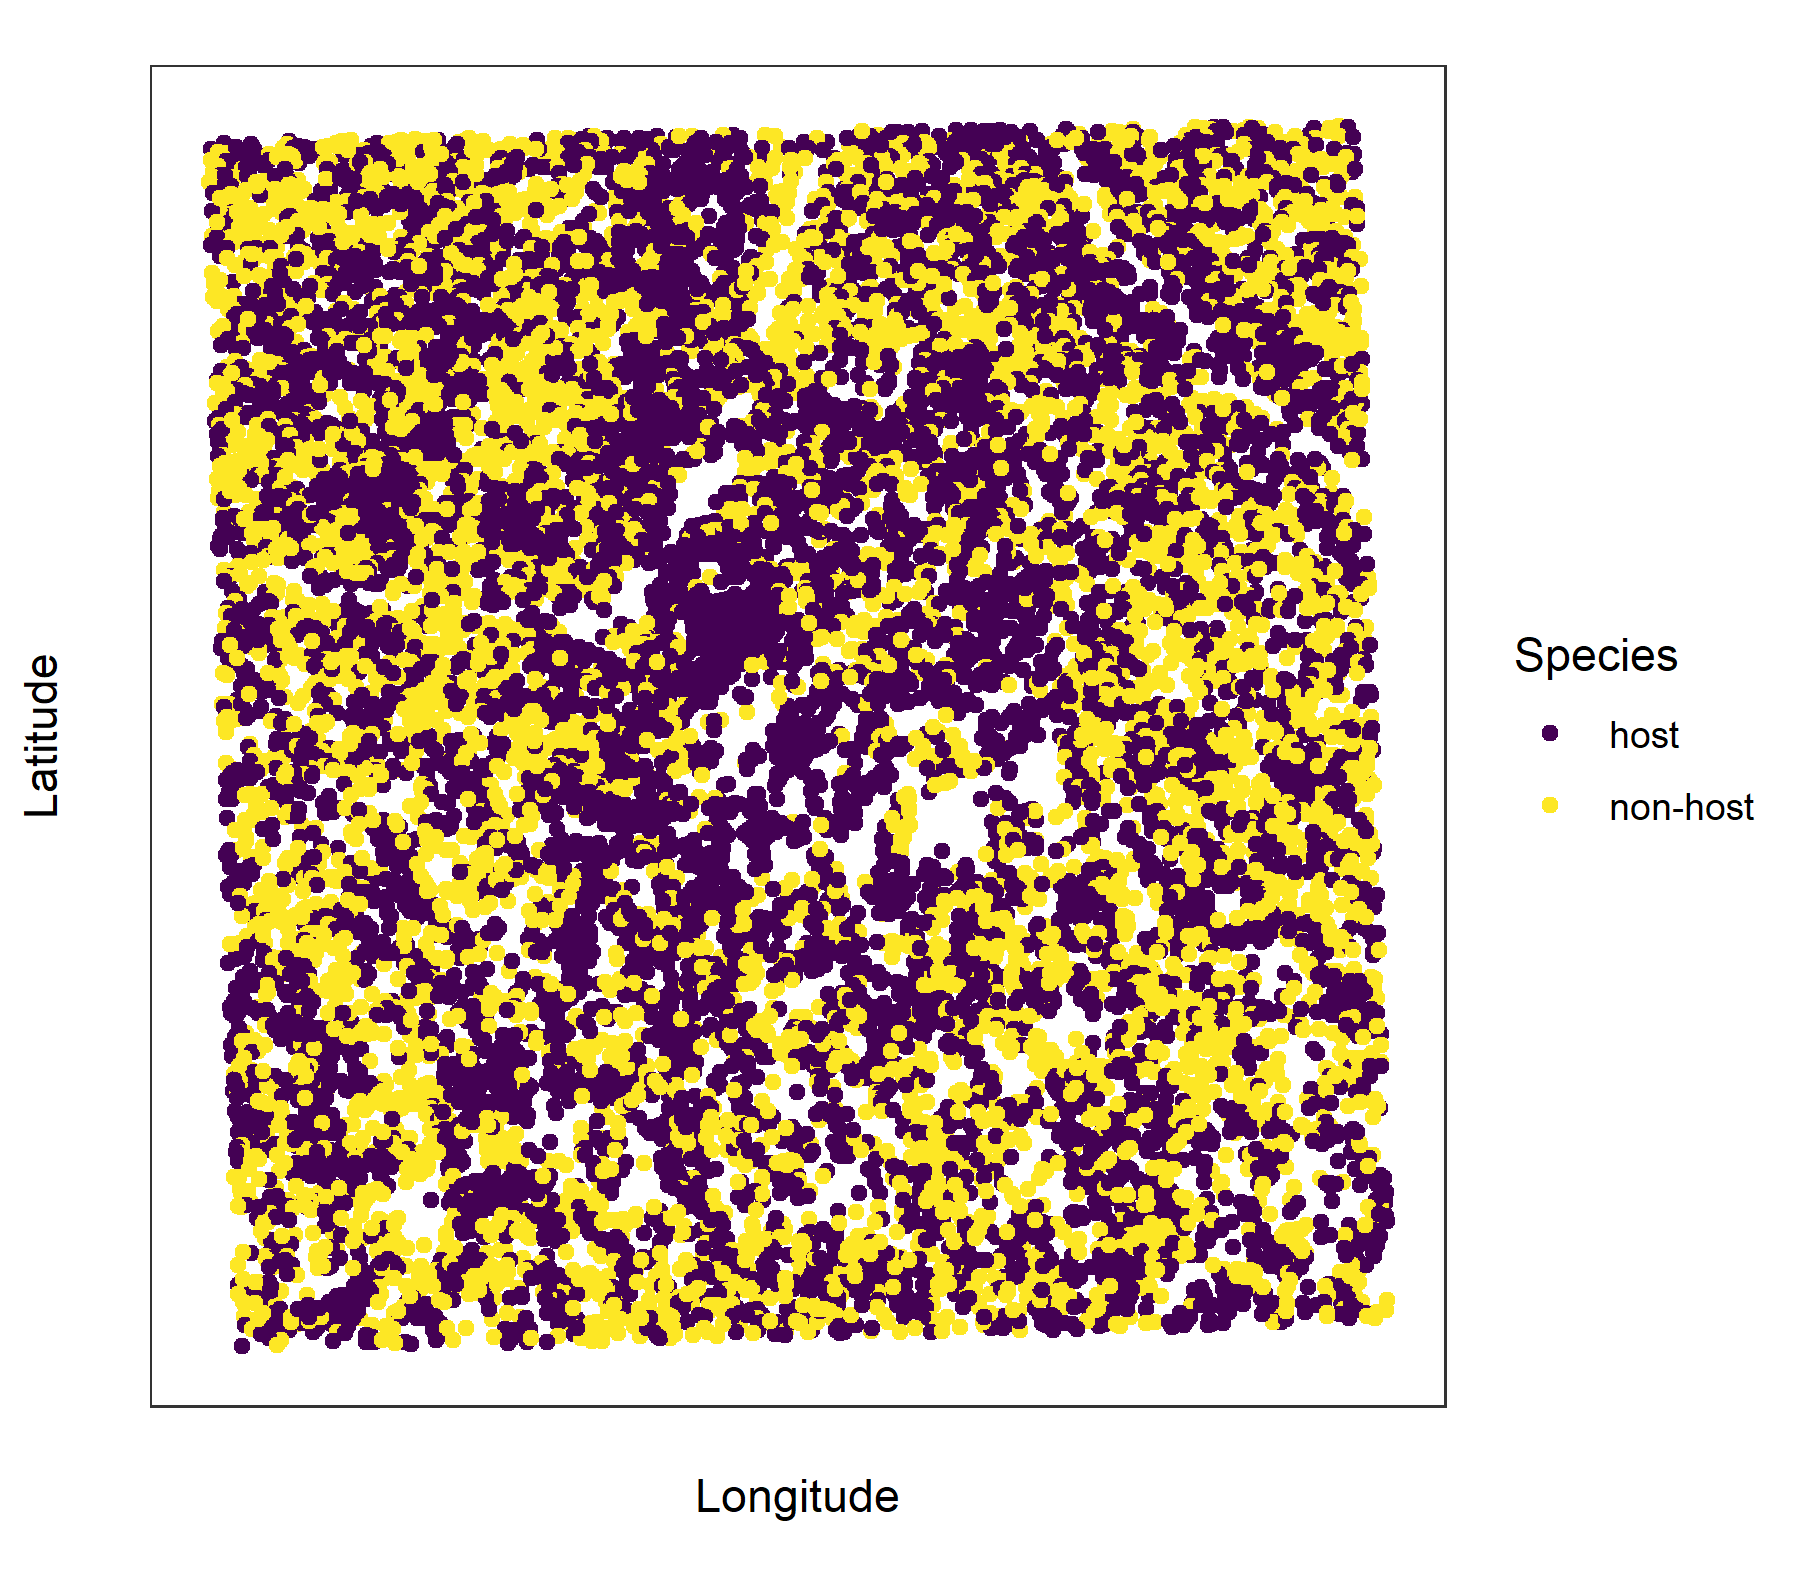
\includegraphics[width=6.00000in]{figure/chap02/eldo_3k_3_host_nonhost.png}
\caption{For each live tree, we classified its species using the same
means of extracted pixel values across the 5 Rededge3 narrow bands (and
5 derived bands) as predictors in a regularized discriminant analysis
previously trained on a hand-classified set of segmented crowns from
across the study area.}
\end{figure}
We overlaid the segmented crowns on the reflectance maps from 20 sites
spanning the latitudinal and elevation gradient in the study. Using
QGIS, we hand classified 564 trees as live/dead (Figure 2.9) and as one
of 5 dominant species in the study area (\emph{Pinus ponderosa},
\emph{Pinus lambertiana}, \emph{Abies concolor}, \emph{Calocedrus
decurrens}, or \emph{Quercus kelloggi}) using the mapped ground data as
a guide. We treated all trees classified as ponderosa pine as a ``host''
tree and all other species as ``non-host'' trees (Figure 2.10).

We used all 10 mean values of the reflectance bands for each tree crown
polygon to predict whether the hand classified trees were alive or dead
using a boosted logistic regression model implemented in the
\texttt{caret} package (accuracy of live/dead classification on a
withheld test dataset: 97.3\%) (Kuhn
\protect\hyperlink{ref-kuhn2008}{2008}). For just the living trees, we
similarly used all 10 reflectance values to predict the tree species
using regularized discriminant analysis implemented in the
\texttt{caret} package (accuracy of species classification on a withheld
testing dataset: 66.7\%; accuracy of WPB host/non-WPB-host (i.e.,
ponderosa pine versus other tree species) on a withheld testing dataset:
74.4\%).

Finally, we used these models to classify all tree crowns in the data
set as alive or dead as well as the species of living trees.

\subsection{Allometric scaling of height to quadratic mean
diameter}\label{allometric-scaling-of-height-to-quadratic-mean-diameter}

We converted the height of each tree determined using the canopy height
model to its diameter at breast height, 1.37m (DBH). Using the tree
height and DBH ground data from Fettig et al.
(\protect\hyperlink{ref-fettig2019}{2019}), we fit a simple linear
regression to predict DBH from height for each of the 5 dominant
species. Using the model-classified tree species of each segmented tree,
we used the corresponding linear relationship for that species to
estimate the DBH given the tree's height. We then calculated the
quadratic mean diameter for each 20m x 20m cell as the square root of
the average squared diameter of trees within the cell.

\subsection{Note on assumptions about dead
trees}\label{note-on-assumptions-about-dead-trees}

For the purposes of this study, we assumed that all dead trees were
ponderosa pine and were thus host trees for the western pine beetle.
This is a reasonably good assumption for our study area, given that
Fettig et al. (\protect\hyperlink{ref-fettig2019}{2019}) found that
73.4\% of the dead trees in the coincident ground plots were ponderosa
pine. The species contributing to the next highest proportion of dead
trees was incense cedar which represented 18.72\% of the dead trees in
the ground plots. Incense cedar is not a potential host of the western
pine beetle, and different forest structure/environment conditions can
dictate the dynamic between forest insects and their host tree species
(Stephenson et al. \protect\hyperlink{ref-stephenson2019}{2019}). While
the detected mortality is most likely to be ponderosa pine, it is
critical to interpret our results with this known limitation in mind.

\subsection{Rasterizing individual tree
data}\label{rasterizing-individual-tree-data}
\begin{figure}
\centering
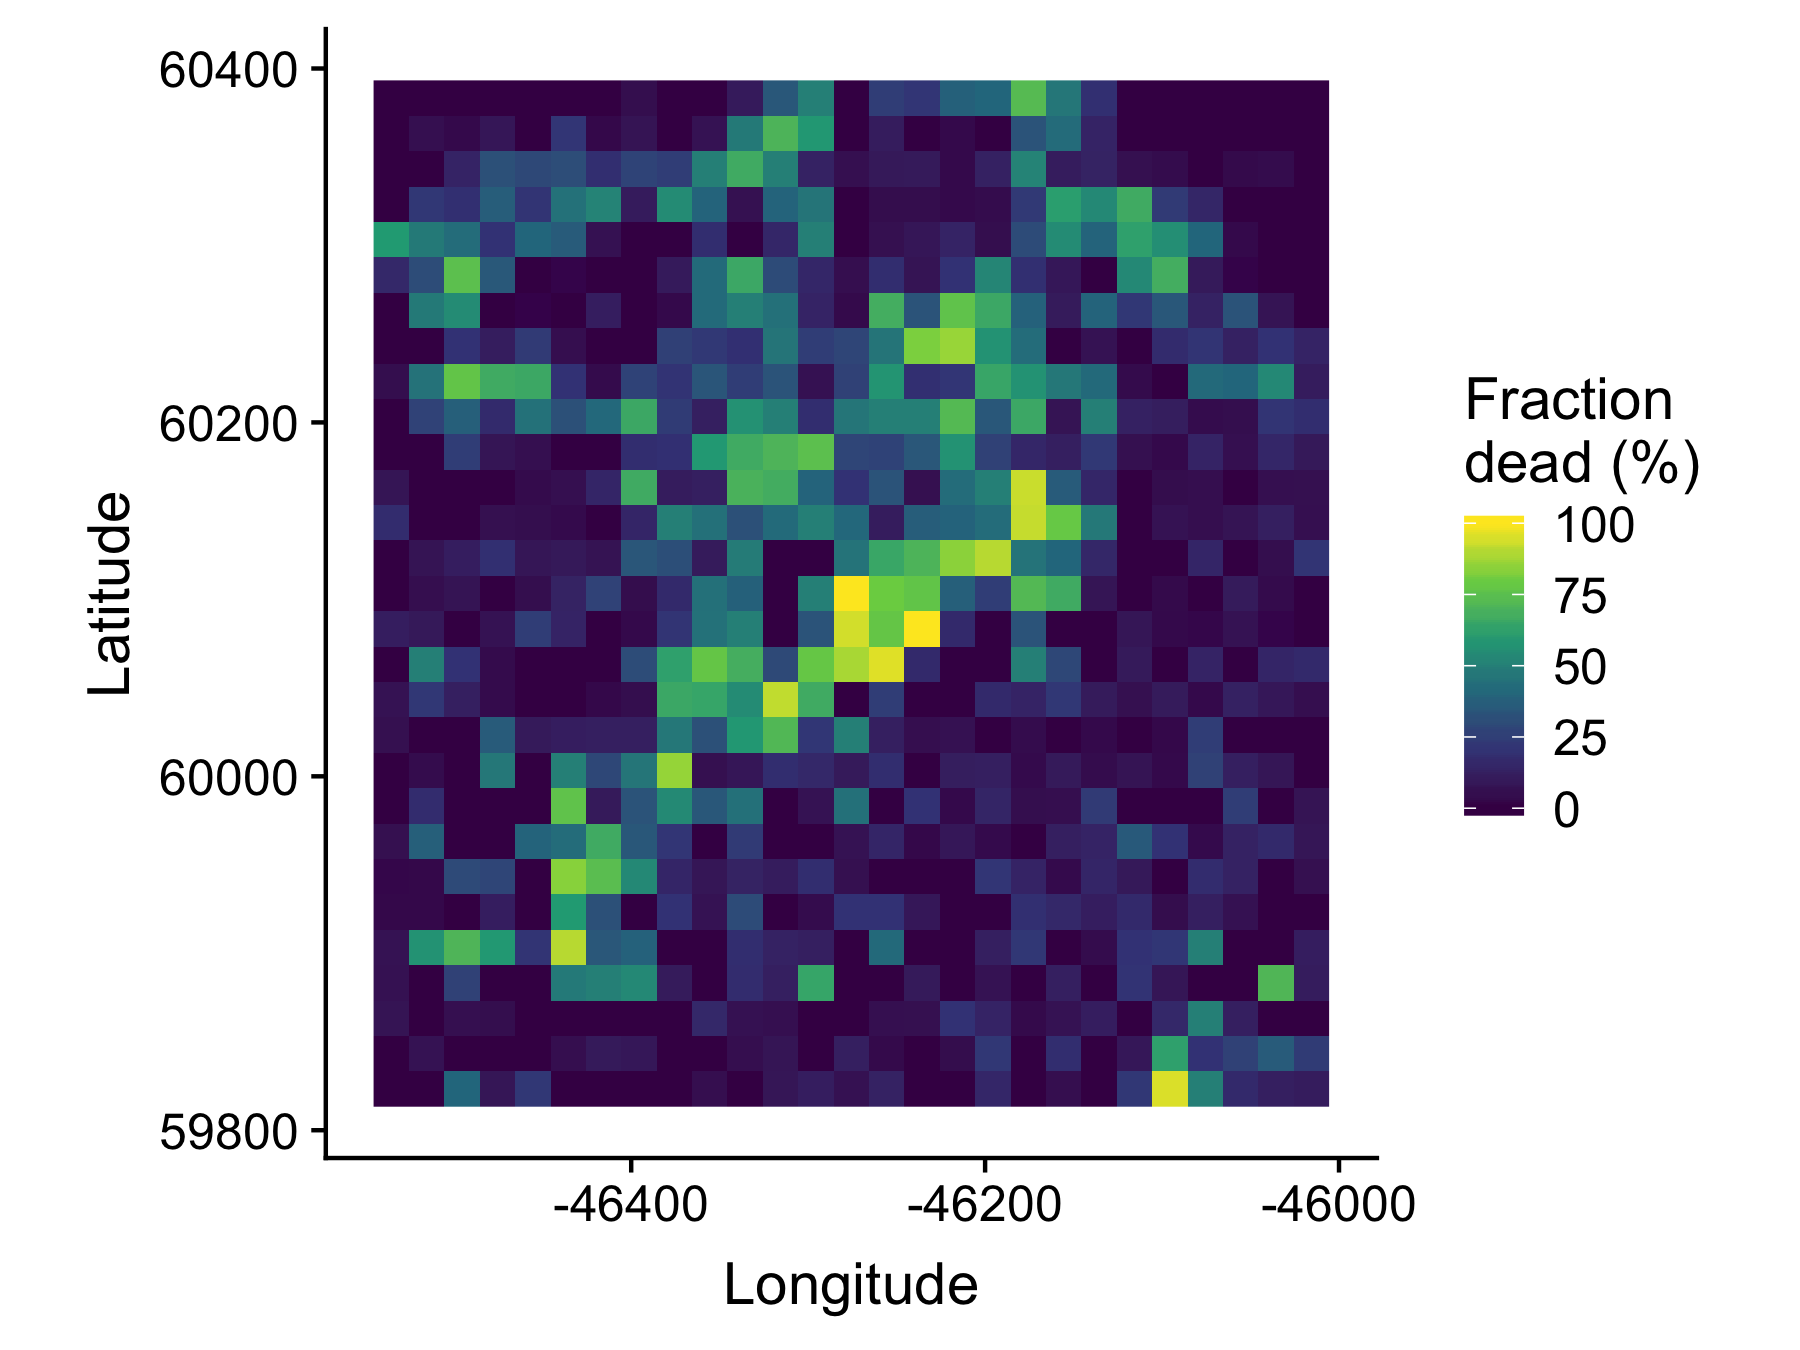
\includegraphics[width=6.00000in]{figure/chap02/proportion-dead-rasterized.png}
\caption{We rasterized the individual tree data by aggregating values to
20m x 20m cells. This example shows the proportion of dead trees per
cell for the same example site as in the previous figures.}
\end{figure}
Because the tree detection algorithms were validated against ground data
at the plot level, we rasterized the classified trees at a spatial
resolution similar to that of the ground plots (Figure 2.11). That is,
we rasterized the individual tree data to 20m x 20m pixels equaling 400
m\textsuperscript{2}, and the circular ground plots with 11.35m radius
covered 404 m\textsuperscript{2}. In each raster cell, we calculated
the: number of live trees, number of dead trees, number of ponderosa
pine trees, total number of trees (of all species, including ponderosa
pine), quadratic mean diameter (QMD) of ponderosa pine trees, and QMD of
all trees of any species (overall QMD). We converted the count of
ponderosa pine trees and the total tree count to a density measurement
of trees per hectare (tpha) by multiplying the counts in each 20m x 20m
cell by 25 to create a ``host density'' and an ``overall density''
variable per cell.

\subsection{Environmental data}\label{environmental-data}

We used climatic water deficit (CWD) (Stephenson
\protect\hyperlink{ref-stephenson1998}{1998}) from the 1981-2010 mean
value of the basin characterization model (Flint et al.
\protect\hyperlink{ref-flint2013}{2013}) as an integrated measure of
temperature and moisture conditions for each of the 32 sites. Higher
values of CWD correspond to hotter, drier conditions and lower values
correspond to cooler, wetter conditions. CWD has been shown to correlate
well with broad patterns of tree mortality in the Sierra Nevada (Young
et al. \protect\hyperlink{ref-young2017}{2017}) as well as bark
beetle-induced tree mortality (Millar et al.
\protect\hyperlink{ref-millar2012}{2012}). We converted the CWD value
for each site into a z-score representing that site's deviation from the
mean CWD across the climatic range of Sierra Nevada ponderosa pine as
determined from 179 herbarium records described in Baldwin et al.
(\protect\hyperlink{ref-baldwin2017a}{2017}). Thus, a CWD z-score of one
would indicate that the CWD at that site is one standard deviation
hotter/drier than the mean CWD across all geolocated herbarium records
for ponderosa pine in the Sierra Nevada.

\subsection{Statistical model}\label{statistical-model}

We used a generalized linear model with a zero-inflated binomial
response and a logit link to predict the probability of ponderosa pine
mortality within each 20m x 20m cell as a function of the crossed
effects of ponderosa pine quadratic mean diameter and density added to
the crossed effect of quadratic mean diameter and density of trees of
all species in each cell (hereafter ``overall quadratic mean diameter''
and ``overall density''), as well as the interaction of each summand
with climatic water deficit at each site.

To measure and account for spatial autocorrelation of the bark beetle
behavioral processes underlying ponderosa pine mortality, we subsampled
the data at each site to a random selection of 200, 20m x 20m cells
representing approximately 27.5\% of the surveyed area. With these
subsampled data, we included a separate exact Gaussian process term per
site of the interaction between the x- and y-position of each cell using
the \texttt{gp()} function in the \texttt{brms} package (Bürkner
\protect\hyperlink{ref-burkner2017}{2017}). The Gaussian process
estimates the spatial covariance in the response variable (log-odds of
ponderosa pine mortality) jointly with the effects of the other
covariates.

\[
\begin{aligned}
y_{i,j} \sim &\ \begin{cases}
0, & p \\
Binom(n_i, \pi_i), & 1-p
\end{cases} \\
logit(\pi_i) = &\ \beta_0\ + \\
& \beta_1X_{cwd, j}\ + \\
& \beta_1X_{cwd, j}(\beta_2X_{pipoQMD, i} + \beta_3X_{pipoDensity, i} + \beta_4X_{pipoQMD, i}X_{pipoDensity, i})\ + \\ 
& \beta_1X_{cwd, j}(\beta_5X_{overallQMD, i} + \beta_6X_{overallDensity, i} + \beta_7X_{overallQMD, i}X_{overallDensity, i})\ + \\
& \mathcal{GP}_j(x_i, y_i) \\
\end{aligned}
\]

Where \(y_i\) is the number of dead trees in cell \(i\), \(n_i\) is the
sum of the dead trees (assumed to be ponderosa pine) and live ponderosa
pine trees in cell \(i\), \(\pi_i\) is the probability of ponderosa pine
tree mortality in cell \(i\), \(p\) is the probability of there being
zero dead trees in a cell arising as a result of an unmodeled process,
\(X_{cwd, j}\) is the z-score of climatic water deficit for site \(j\),
\(X_{pipoQMD, i}\) is the scaled quadratic mean diameter of ponderosa
pine in cell \(i\), \(X_{pipoDensity, i}\) is the scaled density of
ponderosa pine trees in cell \(i\), \(X_{overallQMD, i}\) is the scaled
quadratic mean diameter of all trees in cell \(i\),
\(X_{overallDensity, i}\) is the scaled density of all trees in cell
\(i\), \(x_i\) and \(y_i\) are the x- and y- coordinates of the centroid
of the cell in an EPSG3310 coordinate reference system, and
\(\mathcal{GP}_j\) represents the exact Gaussian process describing the
spatial covariance between cells at site \(j\).

We used 4 chains with 2000 iterations each (1000 warmup, 1000 samples),
and confirmed chain convergence by ensuring all \texttt{Rhat} values
were less than 1.1 (Brooks and Gelman
\protect\hyperlink{ref-brooks1998}{1998}). We used posterior predictive
checks to visually confirm model performance by overlaying the density
curves of the predicted number of dead trees per cell over the observed
number (Gabry et al. \protect\hyperlink{ref-gabry2019}{2019}). For the
posterior predictive checks, we used 50 random samples from the model
fit to generate 50 density curves and ensured curves were centered on
the observed distribution, paying special attention to model performance
at capturing counts of zero.

\subsection{Software and data
availability}\label{software-and-data-availability}

All data are available via the Open Science Framework. Statistical
analyses were performed using the \texttt{brms} packages. With the
exception of the SfM software (Pix4Dmapper Cloud) and the GIS software
QGIS, all data carpentry and analyses were performed using \texttt{R} (R
Core Team \protect\hyperlink{ref-rcoreteam2018}{2018}).

\section{Results}\label{results-1}
\begin{longtable}[]{@{}cccccc@{}}
\caption{Site characteristics for each of the 32 sites. The site name
consists of the forest name, elevation band, and rep separated by an
underscore. The Eldorado National Forest is `eldo', the Stanislaus
National Forest is `stan', the Sierra National Forest is `sier', and the
Sequoia National Forest is `sequ'. The elevation band represents the
lower bounds of the 305 meter (1000 foot) elevation bands in feet. Thus
`3k' implies that site was located between 3,000 and 4,000 feet
(914-1219 meters). Aerially detected mortality and density of the whole
site is presented along with the mortality and density calculated from
the ground data (aerial / ground). The density is measured in trees per
hectare (tpha).}\tabularnewline
\toprule
\begin{minipage}[b]{0.11\columnwidth}\centering\strut
Site\strut
\end{minipage} & \begin{minipage}[b]{0.07\columnwidth}\centering\strut
CWD (mm)\strut
\end{minipage} & \begin{minipage}[b]{0.11\columnwidth}\centering\strut
CWD (z-score)\strut
\end{minipage} & \begin{minipage}[b]{0.13\columnwidth}\centering\strut
Survey area (ha)\strut
\end{minipage} & \begin{minipage}[b]{0.18\columnwidth}\centering\strut
\% tree mortality (aerial/ground)\strut
\end{minipage} & \begin{minipage}[b]{0.22\columnwidth}\centering\strut
Density (tpha; aerial/ground)\strut
\end{minipage}\tabularnewline
\midrule
\endfirsthead
\toprule
\begin{minipage}[b]{0.11\columnwidth}\centering\strut
Site\strut
\end{minipage} & \begin{minipage}[b]{0.07\columnwidth}\centering\strut
CWD (mm)\strut
\end{minipage} & \begin{minipage}[b]{0.11\columnwidth}\centering\strut
CWD (z-score)\strut
\end{minipage} & \begin{minipage}[b]{0.13\columnwidth}\centering\strut
Survey area (ha)\strut
\end{minipage} & \begin{minipage}[b]{0.18\columnwidth}\centering\strut
\% tree mortality (aerial/ground)\strut
\end{minipage} & \begin{minipage}[b]{0.22\columnwidth}\centering\strut
Density (tpha; aerial/ground)\strut
\end{minipage}\tabularnewline
\midrule
\endhead
\begin{minipage}[t]{0.11\columnwidth}\centering\strut
eldo\_3k\_1\strut
\end{minipage} & \begin{minipage}[t]{0.07\columnwidth}\centering\strut
678\strut
\end{minipage} & \begin{minipage}[t]{0.11\columnwidth}\centering\strut
0.319\strut
\end{minipage} & \begin{minipage}[t]{0.13\columnwidth}\centering\strut
31.02\strut
\end{minipage} & \begin{minipage}[t]{0.18\columnwidth}\centering\strut
11/61\strut
\end{minipage} & \begin{minipage}[t]{0.22\columnwidth}\centering\strut
630/410\strut
\end{minipage}\tabularnewline
\begin{minipage}[t]{0.11\columnwidth}\centering\strut
eldo\_3k\_2\strut
\end{minipage} & \begin{minipage}[t]{0.07\columnwidth}\centering\strut
706\strut
\end{minipage} & \begin{minipage}[t]{0.11\columnwidth}\centering\strut
0.501\strut
\end{minipage} & \begin{minipage}[t]{0.13\columnwidth}\centering\strut
30.61\strut
\end{minipage} & \begin{minipage}[t]{0.18\columnwidth}\centering\strut
12/36\strut
\end{minipage} & \begin{minipage}[t]{0.22\columnwidth}\centering\strut
444/647\strut
\end{minipage}\tabularnewline
\begin{minipage}[t]{0.11\columnwidth}\centering\strut
eldo\_3k\_3\strut
\end{minipage} & \begin{minipage}[t]{0.07\columnwidth}\centering\strut
655\strut
\end{minipage} & \begin{minipage}[t]{0.11\columnwidth}\centering\strut
0.163\strut
\end{minipage} & \begin{minipage}[t]{0.13\columnwidth}\centering\strut
30.95\strut
\end{minipage} & \begin{minipage}[t]{0.18\columnwidth}\centering\strut
22/36\strut
\end{minipage} & \begin{minipage}[t]{0.22\columnwidth}\centering\strut
493/410\strut
\end{minipage}\tabularnewline
\begin{minipage}[t]{0.11\columnwidth}\centering\strut
eldo\_4k\_1\strut
\end{minipage} & \begin{minipage}[t]{0.07\columnwidth}\centering\strut
570\strut
\end{minipage} & \begin{minipage}[t]{0.11\columnwidth}\centering\strut
-0.383\strut
\end{minipage} & \begin{minipage}[t]{0.13\columnwidth}\centering\strut
28.04\strut
\end{minipage} & \begin{minipage}[t]{0.18\columnwidth}\centering\strut
9/39\strut
\end{minipage} & \begin{minipage}[t]{0.22\columnwidth}\centering\strut
633/588\strut
\end{minipage}\tabularnewline
\begin{minipage}[t]{0.11\columnwidth}\centering\strut
eldo\_4k\_2\strut
\end{minipage} & \begin{minipage}[t]{0.07\columnwidth}\centering\strut
642\strut
\end{minipage} & \begin{minipage}[t]{0.11\columnwidth}\centering\strut
0.0831\strut
\end{minipage} & \begin{minipage}[t]{0.13\columnwidth}\centering\strut
28.41\strut
\end{minipage} & \begin{minipage}[t]{0.18\columnwidth}\centering\strut
15/78\strut
\end{minipage} & \begin{minipage}[t]{0.22\columnwidth}\centering\strut
338/272\strut
\end{minipage}\tabularnewline
\begin{minipage}[t]{0.11\columnwidth}\centering\strut
eldo\_5k\_1\strut
\end{minipage} & \begin{minipage}[t]{0.07\columnwidth}\centering\strut
663\strut
\end{minipage} & \begin{minipage}[t]{0.11\columnwidth}\centering\strut
0.219\strut
\end{minipage} & \begin{minipage}[t]{0.13\columnwidth}\centering\strut
28.44\strut
\end{minipage} & \begin{minipage}[t]{0.18\columnwidth}\centering\strut
11/44\strut
\end{minipage} & \begin{minipage}[t]{0.22\columnwidth}\centering\strut
662/544\strut
\end{minipage}\tabularnewline
\begin{minipage}[t]{0.11\columnwidth}\centering\strut
eldo\_5k\_2\strut
\end{minipage} & \begin{minipage}[t]{0.07\columnwidth}\centering\strut
627\strut
\end{minipage} & \begin{minipage}[t]{0.11\columnwidth}\centering\strut
-0.0132\strut
\end{minipage} & \begin{minipage}[t]{0.13\columnwidth}\centering\strut
30.02\strut
\end{minipage} & \begin{minipage}[t]{0.18\columnwidth}\centering\strut
12/36\strut
\end{minipage} & \begin{minipage}[t]{0.22\columnwidth}\centering\strut
585/969\strut
\end{minipage}\tabularnewline
\begin{minipage}[t]{0.11\columnwidth}\centering\strut
eldo\_5k\_3\strut
\end{minipage} & \begin{minipage}[t]{0.07\columnwidth}\centering\strut
599\strut
\end{minipage} & \begin{minipage}[t]{0.11\columnwidth}\centering\strut
-0.2\strut
\end{minipage} & \begin{minipage}[t]{0.13\columnwidth}\centering\strut
29.73\strut
\end{minipage} & \begin{minipage}[t]{0.18\columnwidth}\centering\strut
7/32\strut
\end{minipage} & \begin{minipage}[t]{0.22\columnwidth}\centering\strut
489/623\strut
\end{minipage}\tabularnewline
\begin{minipage}[t]{0.11\columnwidth}\centering\strut
stan\_3k\_1\strut
\end{minipage} & \begin{minipage}[t]{0.07\columnwidth}\centering\strut
638\strut
\end{minipage} & \begin{minipage}[t]{0.11\columnwidth}\centering\strut
0.059\strut
\end{minipage} & \begin{minipage}[t]{0.13\columnwidth}\centering\strut
31.04\strut
\end{minipage} & \begin{minipage}[t]{0.18\columnwidth}\centering\strut
10/52\strut
\end{minipage} & \begin{minipage}[t]{0.22\columnwidth}\centering\strut
739/1038\strut
\end{minipage}\tabularnewline
\begin{minipage}[t]{0.11\columnwidth}\centering\strut
stan\_3k\_2\strut
\end{minipage} & \begin{minipage}[t]{0.07\columnwidth}\centering\strut
739\strut
\end{minipage} & \begin{minipage}[t]{0.11\columnwidth}\centering\strut
0.713\strut
\end{minipage} & \begin{minipage}[t]{0.13\columnwidth}\centering\strut
18.78\strut
\end{minipage} & \begin{minipage}[t]{0.18\columnwidth}\centering\strut
40/78\strut
\end{minipage} & \begin{minipage}[t]{0.22\columnwidth}\centering\strut
434/405\strut
\end{minipage}\tabularnewline
\begin{minipage}[t]{0.11\columnwidth}\centering\strut
stan\_3k\_3\strut
\end{minipage} & \begin{minipage}[t]{0.07\columnwidth}\centering\strut
762\strut
\end{minipage} & \begin{minipage}[t]{0.11\columnwidth}\centering\strut
0.859\strut
\end{minipage} & \begin{minipage}[t]{0.13\columnwidth}\centering\strut
30.1\strut
\end{minipage} & \begin{minipage}[t]{0.18\columnwidth}\centering\strut
22/41\strut
\end{minipage} & \begin{minipage}[t]{0.22\columnwidth}\centering\strut
558/326\strut
\end{minipage}\tabularnewline
\begin{minipage}[t]{0.11\columnwidth}\centering\strut
stan\_4k\_1\strut
\end{minipage} & \begin{minipage}[t]{0.07\columnwidth}\centering\strut
540\strut
\end{minipage} & \begin{minipage}[t]{0.11\columnwidth}\centering\strut
-0.58\strut
\end{minipage} & \begin{minipage}[t]{0.13\columnwidth}\centering\strut
29.62\strut
\end{minipage} & \begin{minipage}[t]{0.18\columnwidth}\centering\strut
29/63\strut
\end{minipage} & \begin{minipage}[t]{0.22\columnwidth}\centering\strut
508/712\strut
\end{minipage}\tabularnewline
\begin{minipage}[t]{0.11\columnwidth}\centering\strut
stan\_4k\_2\strut
\end{minipage} & \begin{minipage}[t]{0.07\columnwidth}\centering\strut
528\strut
\end{minipage} & \begin{minipage}[t]{0.11\columnwidth}\centering\strut
-0.658\strut
\end{minipage} & \begin{minipage}[t]{0.13\columnwidth}\centering\strut
30.54\strut
\end{minipage} & \begin{minipage}[t]{0.18\columnwidth}\centering\strut
18/56\strut
\end{minipage} & \begin{minipage}[t]{0.22\columnwidth}\centering\strut
482/257\strut
\end{minipage}\tabularnewline
\begin{minipage}[t]{0.11\columnwidth}\centering\strut
stan\_5k\_1\strut
\end{minipage} & \begin{minipage}[t]{0.07\columnwidth}\centering\strut
524\strut
\end{minipage} & \begin{minipage}[t]{0.11\columnwidth}\centering\strut
-0.688\strut
\end{minipage} & \begin{minipage}[t]{0.13\columnwidth}\centering\strut
30.94\strut
\end{minipage} & \begin{minipage}[t]{0.18\columnwidth}\centering\strut
19/54\strut
\end{minipage} & \begin{minipage}[t]{0.22\columnwidth}\centering\strut
389/336\strut
\end{minipage}\tabularnewline
\begin{minipage}[t]{0.11\columnwidth}\centering\strut
stan\_5k\_2\strut
\end{minipage} & \begin{minipage}[t]{0.07\columnwidth}\centering\strut
524\strut
\end{minipage} & \begin{minipage}[t]{0.11\columnwidth}\centering\strut
-0.685\strut
\end{minipage} & \begin{minipage}[t]{0.13\columnwidth}\centering\strut
29.94\strut
\end{minipage} & \begin{minipage}[t]{0.18\columnwidth}\centering\strut
21/44\strut
\end{minipage} & \begin{minipage}[t]{0.22\columnwidth}\centering\strut
399/623\strut
\end{minipage}\tabularnewline
\begin{minipage}[t]{0.11\columnwidth}\centering\strut
sier\_3k\_1\strut
\end{minipage} & \begin{minipage}[t]{0.07\columnwidth}\centering\strut
764\strut
\end{minipage} & \begin{minipage}[t]{0.11\columnwidth}\centering\strut
0.871\strut
\end{minipage} & \begin{minipage}[t]{0.13\columnwidth}\centering\strut
30.42\strut
\end{minipage} & \begin{minipage}[t]{0.18\columnwidth}\centering\strut
19/48\strut
\end{minipage} & \begin{minipage}[t]{0.22\columnwidth}\centering\strut
651/850\strut
\end{minipage}\tabularnewline
\begin{minipage}[t]{0.11\columnwidth}\centering\strut
sier\_3k\_2\strut
\end{minipage} & \begin{minipage}[t]{0.07\columnwidth}\centering\strut
768\strut
\end{minipage} & \begin{minipage}[t]{0.11\columnwidth}\centering\strut
0.898\strut
\end{minipage} & \begin{minipage}[t]{0.13\columnwidth}\centering\strut
30.05\strut
\end{minipage} & \begin{minipage}[t]{0.18\columnwidth}\centering\strut
20/77\strut
\end{minipage} & \begin{minipage}[t]{0.22\columnwidth}\centering\strut
439/153\strut
\end{minipage}\tabularnewline
\begin{minipage}[t]{0.11\columnwidth}\centering\strut
sier\_3k\_3\strut
\end{minipage} & \begin{minipage}[t]{0.07\columnwidth}\centering\strut
773\strut
\end{minipage} & \begin{minipage}[t]{0.11\columnwidth}\centering\strut
0.932\strut
\end{minipage} & \begin{minipage}[t]{0.13\columnwidth}\centering\strut
29.77\strut
\end{minipage} & \begin{minipage}[t]{0.18\columnwidth}\centering\strut
32/77\strut
\end{minipage} & \begin{minipage}[t]{0.22\columnwidth}\centering\strut
511/460\strut
\end{minipage}\tabularnewline
\begin{minipage}[t]{0.11\columnwidth}\centering\strut
sier\_4k\_1\strut
\end{minipage} & \begin{minipage}[t]{0.07\columnwidth}\centering\strut
841\strut
\end{minipage} & \begin{minipage}[t]{0.11\columnwidth}\centering\strut
1.38\strut
\end{minipage} & \begin{minipage}[t]{0.13\columnwidth}\centering\strut
30.43\strut
\end{minipage} & \begin{minipage}[t]{0.18\columnwidth}\centering\strut
54/51\strut
\end{minipage} & \begin{minipage}[t]{0.22\columnwidth}\centering\strut
576/539\strut
\end{minipage}\tabularnewline
\begin{minipage}[t]{0.11\columnwidth}\centering\strut
sier\_4k\_2\strut
\end{minipage} & \begin{minipage}[t]{0.07\columnwidth}\centering\strut
764\strut
\end{minipage} & \begin{minipage}[t]{0.11\columnwidth}\centering\strut
0.877\strut
\end{minipage} & \begin{minipage}[t]{0.13\columnwidth}\centering\strut
29.3\strut
\end{minipage} & \begin{minipage}[t]{0.18\columnwidth}\centering\strut
33/57\strut
\end{minipage} & \begin{minipage}[t]{0.22\columnwidth}\centering\strut
499/855\strut
\end{minipage}\tabularnewline
\begin{minipage}[t]{0.11\columnwidth}\centering\strut
sier\_4k\_3\strut
\end{minipage} & \begin{minipage}[t]{0.07\columnwidth}\centering\strut
688\strut
\end{minipage} & \begin{minipage}[t]{0.11\columnwidth}\centering\strut
0.383\strut
\end{minipage} & \begin{minipage}[t]{0.13\columnwidth}\centering\strut
26.39\strut
\end{minipage} & \begin{minipage}[t]{0.18\columnwidth}\centering\strut
48/59\strut
\end{minipage} & \begin{minipage}[t]{0.22\columnwidth}\centering\strut
454/499\strut
\end{minipage}\tabularnewline
\begin{minipage}[t]{0.11\columnwidth}\centering\strut
sier\_5k\_1\strut
\end{minipage} & \begin{minipage}[t]{0.07\columnwidth}\centering\strut
722\strut
\end{minipage} & \begin{minipage}[t]{0.11\columnwidth}\centering\strut
0.599\strut
\end{minipage} & \begin{minipage}[t]{0.13\columnwidth}\centering\strut
14.59\strut
\end{minipage} & \begin{minipage}[t]{0.18\columnwidth}\centering\strut
41/43\strut
\end{minipage} & \begin{minipage}[t]{0.22\columnwidth}\centering\strut
631/717\strut
\end{minipage}\tabularnewline
\begin{minipage}[t]{0.11\columnwidth}\centering\strut
sier\_5k\_2\strut
\end{minipage} & \begin{minipage}[t]{0.07\columnwidth}\centering\strut
710\strut
\end{minipage} & \begin{minipage}[t]{0.11\columnwidth}\centering\strut
0.523\strut
\end{minipage} & \begin{minipage}[t]{0.13\columnwidth}\centering\strut
27.53\strut
\end{minipage} & \begin{minipage}[t]{0.18\columnwidth}\centering\strut
53/74\strut
\end{minipage} & \begin{minipage}[t]{0.22\columnwidth}\centering\strut
477/455\strut
\end{minipage}\tabularnewline
\begin{minipage}[t]{0.11\columnwidth}\centering\strut
sier\_5k\_3\strut
\end{minipage} & \begin{minipage}[t]{0.07\columnwidth}\centering\strut
779\strut
\end{minipage} & \begin{minipage}[t]{0.11\columnwidth}\centering\strut
0.968\strut
\end{minipage} & \begin{minipage}[t]{0.13\columnwidth}\centering\strut
28.93\strut
\end{minipage} & \begin{minipage}[t]{0.18\columnwidth}\centering\strut
33/43\strut
\end{minipage} & \begin{minipage}[t]{0.22\columnwidth}\centering\strut
569/484\strut
\end{minipage}\tabularnewline
\begin{minipage}[t]{0.11\columnwidth}\centering\strut
sequ\_4k\_1\strut
\end{minipage} & \begin{minipage}[t]{0.07\columnwidth}\centering\strut
767\strut
\end{minipage} & \begin{minipage}[t]{0.11\columnwidth}\centering\strut
0.891\strut
\end{minipage} & \begin{minipage}[t]{0.13\columnwidth}\centering\strut
29.59\strut
\end{minipage} & \begin{minipage}[t]{0.18\columnwidth}\centering\strut
50/56\strut
\end{minipage} & \begin{minipage}[t]{0.22\columnwidth}\centering\strut
366/608\strut
\end{minipage}\tabularnewline
\begin{minipage}[t]{0.11\columnwidth}\centering\strut
sequ\_4k\_3\strut
\end{minipage} & \begin{minipage}[t]{0.07\columnwidth}\centering\strut
816\strut
\end{minipage} & \begin{minipage}[t]{0.11\columnwidth}\centering\strut
1.21\strut
\end{minipage} & \begin{minipage}[t]{0.13\columnwidth}\centering\strut
29.69\strut
\end{minipage} & \begin{minipage}[t]{0.18\columnwidth}\centering\strut
35/71\strut
\end{minipage} & \begin{minipage}[t]{0.22\columnwidth}\centering\strut
433/306\strut
\end{minipage}\tabularnewline
\begin{minipage}[t]{0.11\columnwidth}\centering\strut
sequ\_5k\_1\strut
\end{minipage} & \begin{minipage}[t]{0.07\columnwidth}\centering\strut
718\strut
\end{minipage} & \begin{minipage}[t]{0.11\columnwidth}\centering\strut
0.577\strut
\end{minipage} & \begin{minipage}[t]{0.13\columnwidth}\centering\strut
27.12\strut
\end{minipage} & \begin{minipage}[t]{0.18\columnwidth}\centering\strut
35/52\strut
\end{minipage} & \begin{minipage}[t]{0.22\columnwidth}\centering\strut
364/445\strut
\end{minipage}\tabularnewline
\begin{minipage}[t]{0.11\columnwidth}\centering\strut
sequ\_5k\_2\strut
\end{minipage} & \begin{minipage}[t]{0.07\columnwidth}\centering\strut
587\strut
\end{minipage} & \begin{minipage}[t]{0.11\columnwidth}\centering\strut
-0.274\strut
\end{minipage} & \begin{minipage}[t]{0.13\columnwidth}\centering\strut
29.1\strut
\end{minipage} & \begin{minipage}[t]{0.18\columnwidth}\centering\strut
45/43\strut
\end{minipage} & \begin{minipage}[t]{0.22\columnwidth}\centering\strut
478/499\strut
\end{minipage}\tabularnewline
\begin{minipage}[t]{0.11\columnwidth}\centering\strut
sequ\_5k\_3\strut
\end{minipage} & \begin{minipage}[t]{0.07\columnwidth}\centering\strut
611\strut
\end{minipage} & \begin{minipage}[t]{0.11\columnwidth}\centering\strut
-0.117\strut
\end{minipage} & \begin{minipage}[t]{0.13\columnwidth}\centering\strut
31.34\strut
\end{minipage} & \begin{minipage}[t]{0.18\columnwidth}\centering\strut
42/48\strut
\end{minipage} & \begin{minipage}[t]{0.22\columnwidth}\centering\strut
349/494\strut
\end{minipage}\tabularnewline
\begin{minipage}[t]{0.11\columnwidth}\centering\strut
sequ\_6k\_1\strut
\end{minipage} & \begin{minipage}[t]{0.07\columnwidth}\centering\strut
731\strut
\end{minipage} & \begin{minipage}[t]{0.11\columnwidth}\centering\strut
0.657\strut
\end{minipage} & \begin{minipage}[t]{0.13\columnwidth}\centering\strut
27.78\strut
\end{minipage} & \begin{minipage}[t]{0.18\columnwidth}\centering\strut
30/70\strut
\end{minipage} & \begin{minipage}[t]{0.22\columnwidth}\centering\strut
433/361\strut
\end{minipage}\tabularnewline
\begin{minipage}[t]{0.11\columnwidth}\centering\strut
sequ\_6k\_2\strut
\end{minipage} & \begin{minipage}[t]{0.07\columnwidth}\centering\strut
690\strut
\end{minipage} & \begin{minipage}[t]{0.11\columnwidth}\centering\strut
0.39\strut
\end{minipage} & \begin{minipage}[t]{0.13\columnwidth}\centering\strut
11.83\strut
\end{minipage} & \begin{minipage}[t]{0.18\columnwidth}\centering\strut
26/43\strut
\end{minipage} & \begin{minipage}[t]{0.22\columnwidth}\centering\strut
699/934\strut
\end{minipage}\tabularnewline
\begin{minipage}[t]{0.11\columnwidth}\centering\strut
sequ\_6k\_3\strut
\end{minipage} & \begin{minipage}[t]{0.07\columnwidth}\centering\strut
603\strut
\end{minipage} & \begin{minipage}[t]{0.11\columnwidth}\centering\strut
-0.174\strut
\end{minipage} & \begin{minipage}[t]{0.13\columnwidth}\centering\strut
26.51\strut
\end{minipage} & \begin{minipage}[t]{0.18\columnwidth}\centering\strut
36/32\strut
\end{minipage} & \begin{minipage}[t]{0.22\columnwidth}\centering\strut
536/692\strut
\end{minipage}\tabularnewline
\bottomrule
\end{longtable}
\subsection{Tree detection}\label{tree-detection-1}

We found that the experimental \texttt{lmfx} algorithm with parameter
values of \texttt{dist2d\ =\ 1} and \texttt{ws\ =\ 2.5} (Roussel et al.
\protect\hyperlink{ref-roussel2019}{2019}) performed the best across 7
measures of forest structure as measured by Pearson's correlation with
ground data (Table 2.4).
\begin{longtable}[]{@{}ccccc@{}}
\caption{Correlation and differences between the best performing tree
detection algorithm (lmfx with dist2d = 1 and ws = 2.5) and the ground
data. An asterisk next to the correlation or RMSE indicates that this
value was within 5\% of the value of the best-performing
algorithm/parameter set. Ground mean represents the mean value of the
forest metric across the 110 ground plots that were visible from the
sUAS-derived imagery. The median error is calculated as the median of
the differences between the air and ground values for the 110 visible
plots. Thus, a positive number indicates an overestimate by the sUAS
workflow and a negative number indicates an
underestimate.}\tabularnewline
\toprule
\begin{minipage}[b]{0.28\columnwidth}\centering\strut
Forest structure metric\strut
\end{minipage} & \begin{minipage}[b]{0.13\columnwidth}\centering\strut
Ground mean\strut
\end{minipage} & \begin{minipage}[b]{0.24\columnwidth}\centering\strut
Correlation with ground\strut
\end{minipage} & \begin{minipage}[b]{0.08\columnwidth}\centering\strut
RMSE\strut
\end{minipage} & \begin{minipage}[b]{0.13\columnwidth}\centering\strut
Median error\strut
\end{minipage}\tabularnewline
\midrule
\endfirsthead
\toprule
\begin{minipage}[b]{0.28\columnwidth}\centering\strut
Forest structure metric\strut
\end{minipage} & \begin{minipage}[b]{0.13\columnwidth}\centering\strut
Ground mean\strut
\end{minipage} & \begin{minipage}[b]{0.24\columnwidth}\centering\strut
Correlation with ground\strut
\end{minipage} & \begin{minipage}[b]{0.08\columnwidth}\centering\strut
RMSE\strut
\end{minipage} & \begin{minipage}[b]{0.13\columnwidth}\centering\strut
Median error\strut
\end{minipage}\tabularnewline
\midrule
\endhead
\begin{minipage}[t]{0.28\columnwidth}\centering\strut
total tree count\strut
\end{minipage} & \begin{minipage}[t]{0.13\columnwidth}\centering\strut
19\strut
\end{minipage} & \begin{minipage}[t]{0.24\columnwidth}\centering\strut
0.67*\strut
\end{minipage} & \begin{minipage}[t]{0.08\columnwidth}\centering\strut
8.68*\strut
\end{minipage} & \begin{minipage}[t]{0.13\columnwidth}\centering\strut
2\strut
\end{minipage}\tabularnewline
\begin{minipage}[t]{0.28\columnwidth}\centering\strut
count of trees \textgreater{} 15m\strut
\end{minipage} & \begin{minipage}[t]{0.13\columnwidth}\centering\strut
9.9\strut
\end{minipage} & \begin{minipage}[t]{0.24\columnwidth}\centering\strut
0.43\strut
\end{minipage} & \begin{minipage}[t]{0.08\columnwidth}\centering\strut
7.38\strut
\end{minipage} & \begin{minipage}[t]{0.13\columnwidth}\centering\strut
0\strut
\end{minipage}\tabularnewline
\begin{minipage}[t]{0.28\columnwidth}\centering\strut
distance to 1st neighbor (m)\strut
\end{minipage} & \begin{minipage}[t]{0.13\columnwidth}\centering\strut
2.8\strut
\end{minipage} & \begin{minipage}[t]{0.24\columnwidth}\centering\strut
0.55*\strut
\end{minipage} & \begin{minipage}[t]{0.08\columnwidth}\centering\strut
1.16*\strut
\end{minipage} & \begin{minipage}[t]{0.13\columnwidth}\centering\strut
0.26\strut
\end{minipage}\tabularnewline
\begin{minipage}[t]{0.28\columnwidth}\centering\strut
distance to 2nd neighbor (m)\strut
\end{minipage} & \begin{minipage}[t]{0.13\columnwidth}\centering\strut
4.3\strut
\end{minipage} & \begin{minipage}[t]{0.24\columnwidth}\centering\strut
0.61*\strut
\end{minipage} & \begin{minipage}[t]{0.08\columnwidth}\centering\strut
1.70*\strut
\end{minipage} & \begin{minipage}[t]{0.13\columnwidth}\centering\strut
0.12\strut
\end{minipage}\tabularnewline
\begin{minipage}[t]{0.28\columnwidth}\centering\strut
height (m); 25th percentile\strut
\end{minipage} & \begin{minipage}[t]{0.13\columnwidth}\centering\strut
12\strut
\end{minipage} & \begin{minipage}[t]{0.24\columnwidth}\centering\strut
0.16\strut
\end{minipage} & \begin{minipage}[t]{0.08\columnwidth}\centering\strut
8.46\strut
\end{minipage} & \begin{minipage}[t]{0.13\columnwidth}\centering\strut
-1.2\strut
\end{minipage}\tabularnewline
\begin{minipage}[t]{0.28\columnwidth}\centering\strut
height (m); mean\strut
\end{minipage} & \begin{minipage}[t]{0.13\columnwidth}\centering\strut
18\strut
\end{minipage} & \begin{minipage}[t]{0.24\columnwidth}\centering\strut
0.29\strut
\end{minipage} & \begin{minipage}[t]{0.08\columnwidth}\centering\strut
7.81*\strut
\end{minipage} & \begin{minipage}[t]{0.13\columnwidth}\centering\strut
-2.3\strut
\end{minipage}\tabularnewline
\begin{minipage}[t]{0.28\columnwidth}\centering\strut
height (m); 75th percentile\strut
\end{minipage} & \begin{minipage}[t]{0.13\columnwidth}\centering\strut
25\strut
\end{minipage} & \begin{minipage}[t]{0.24\columnwidth}\centering\strut
0.35\strut
\end{minipage} & \begin{minipage}[t]{0.08\columnwidth}\centering\strut
10.33*\strut
\end{minipage} & \begin{minipage}[t]{0.13\columnwidth}\centering\strut
-4\strut
\end{minipage}\tabularnewline
\bottomrule
\end{longtable}
\subsection{Effect of local structure and regional climate on western
pine beetle
severity}\label{effect-of-local-structure-and-regional-climate-on-western-pine-beetle-severity}
\begin{figure}
\centering
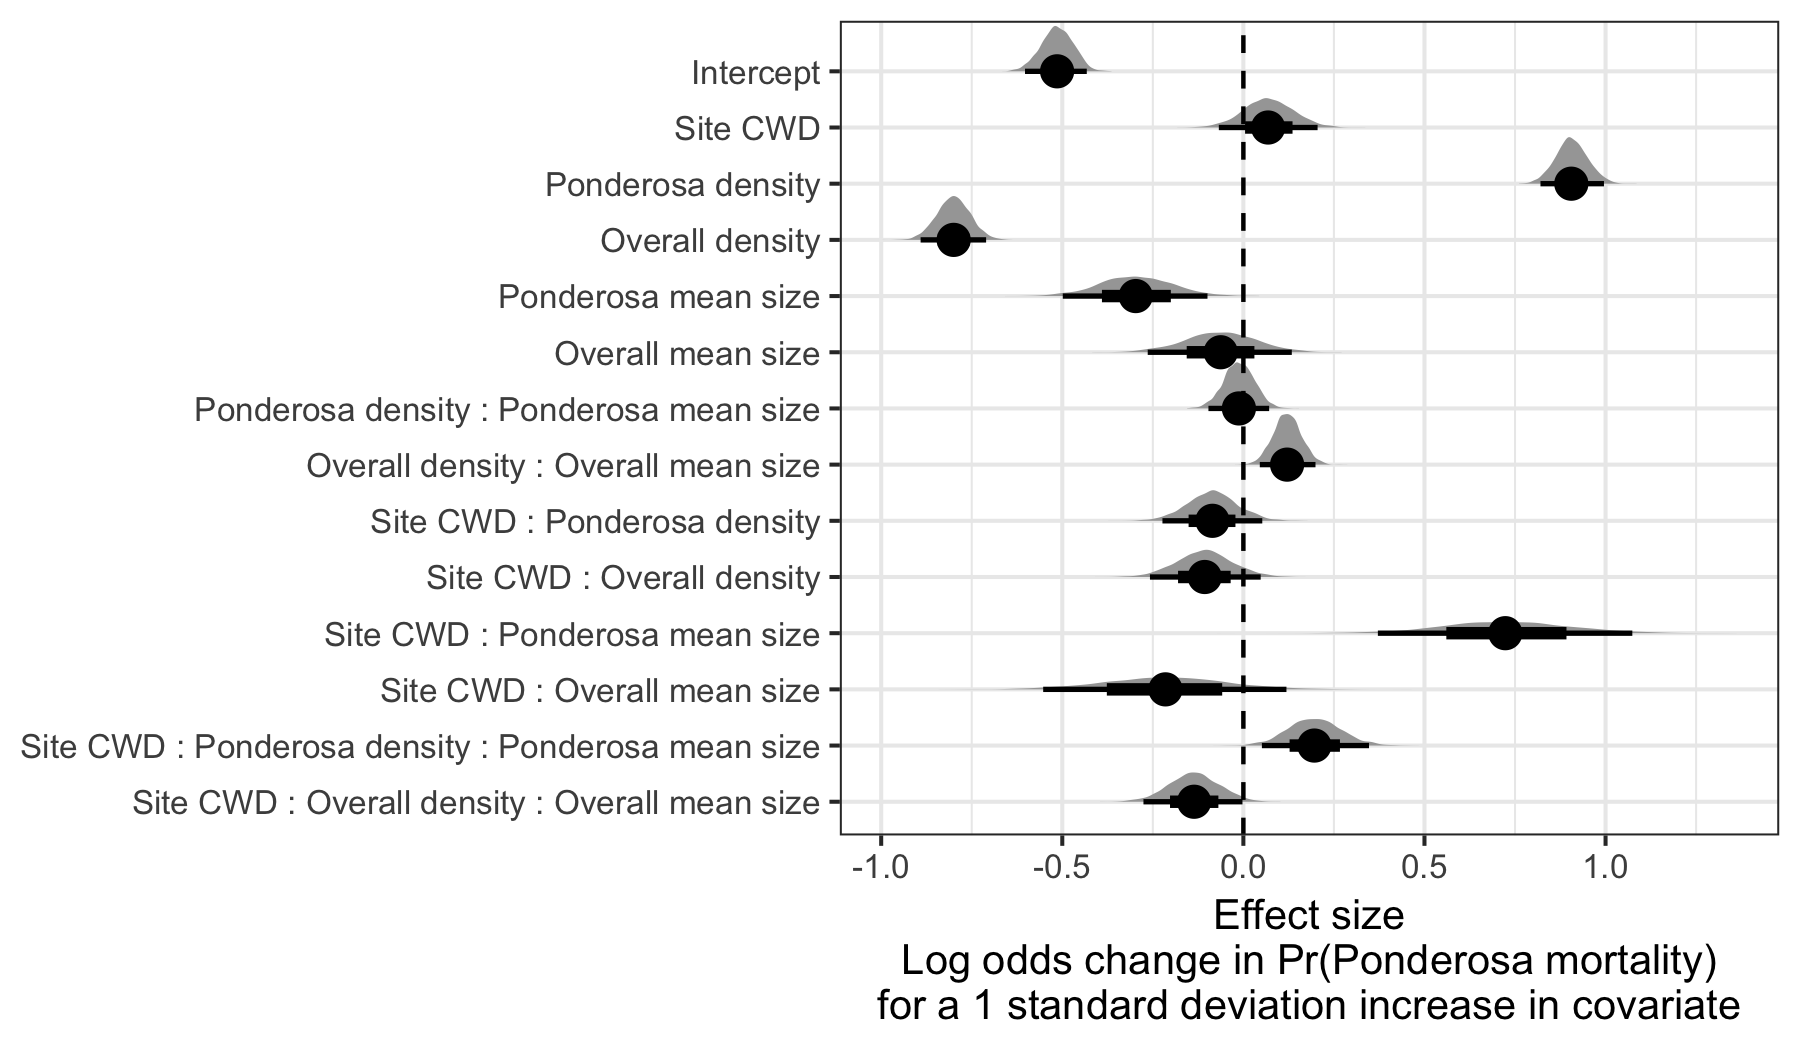
\includegraphics[width=6.00000in]{figure/chap02/effect-sizes-halfeye.png}
\caption{Posterior distributions of effect size from zero-inflated
binomial model predicting the probability of ponderosa pine mortality in
a 20m x 20m cell given forest structure characteristics of host trees
and all trees within the cell, as well as a site-level climatic water
deficit. The gray density distribution for each model covariate
represents the density of the posterior distribution, the point
underneath each density curve represents the median of the estimate, the
bold interval surrounding the point estimate represents the 66\%
credible interval, and the thin interval surrounding the point estimate
represents the 95\% credible interval.}
\end{figure}
We detected a small, generally positive main effect of climatic water
deficit on the probability of ponderosa pine mortality within each 20m x
20m cell (Figure 2.12).

We found a strongly positive main effect of ponderosa pine local
density, with greater density increasing the probability of ponderosa
pine mortality. Conversely, we found a strong negative effect of overall
tree density (i.e., including both ponderosa pine and non-host species)
such that additional non-host trees in a 20m x 20m cell (for the same
number of host trees) would decrease the probability of ponderosa pine
mortality (Figure 2.12).

We found a generally negative effect of quadratic mean diameter of
ponderosa pine on the probability of ponderosa mortality, suggesting
that the western pine beetle attacked smaller trees, on average. There
was a strong positive interaction between the climatic water deficit and
ponderosa pine quadratic mean diameter, such that larger trees were more
likely to increase the probability of ponderosa mortality in hotter,
drier sites (Figure 2.13).

There was a positive interaction between overall tree density and
overall quadratic mean diameter, such that denser stands with larger
trees did lead to greater ponderosa pine mortality, though the main
effects of each of these variables were weakly negative (Figure 2.12).
\begin{figure}
\centering
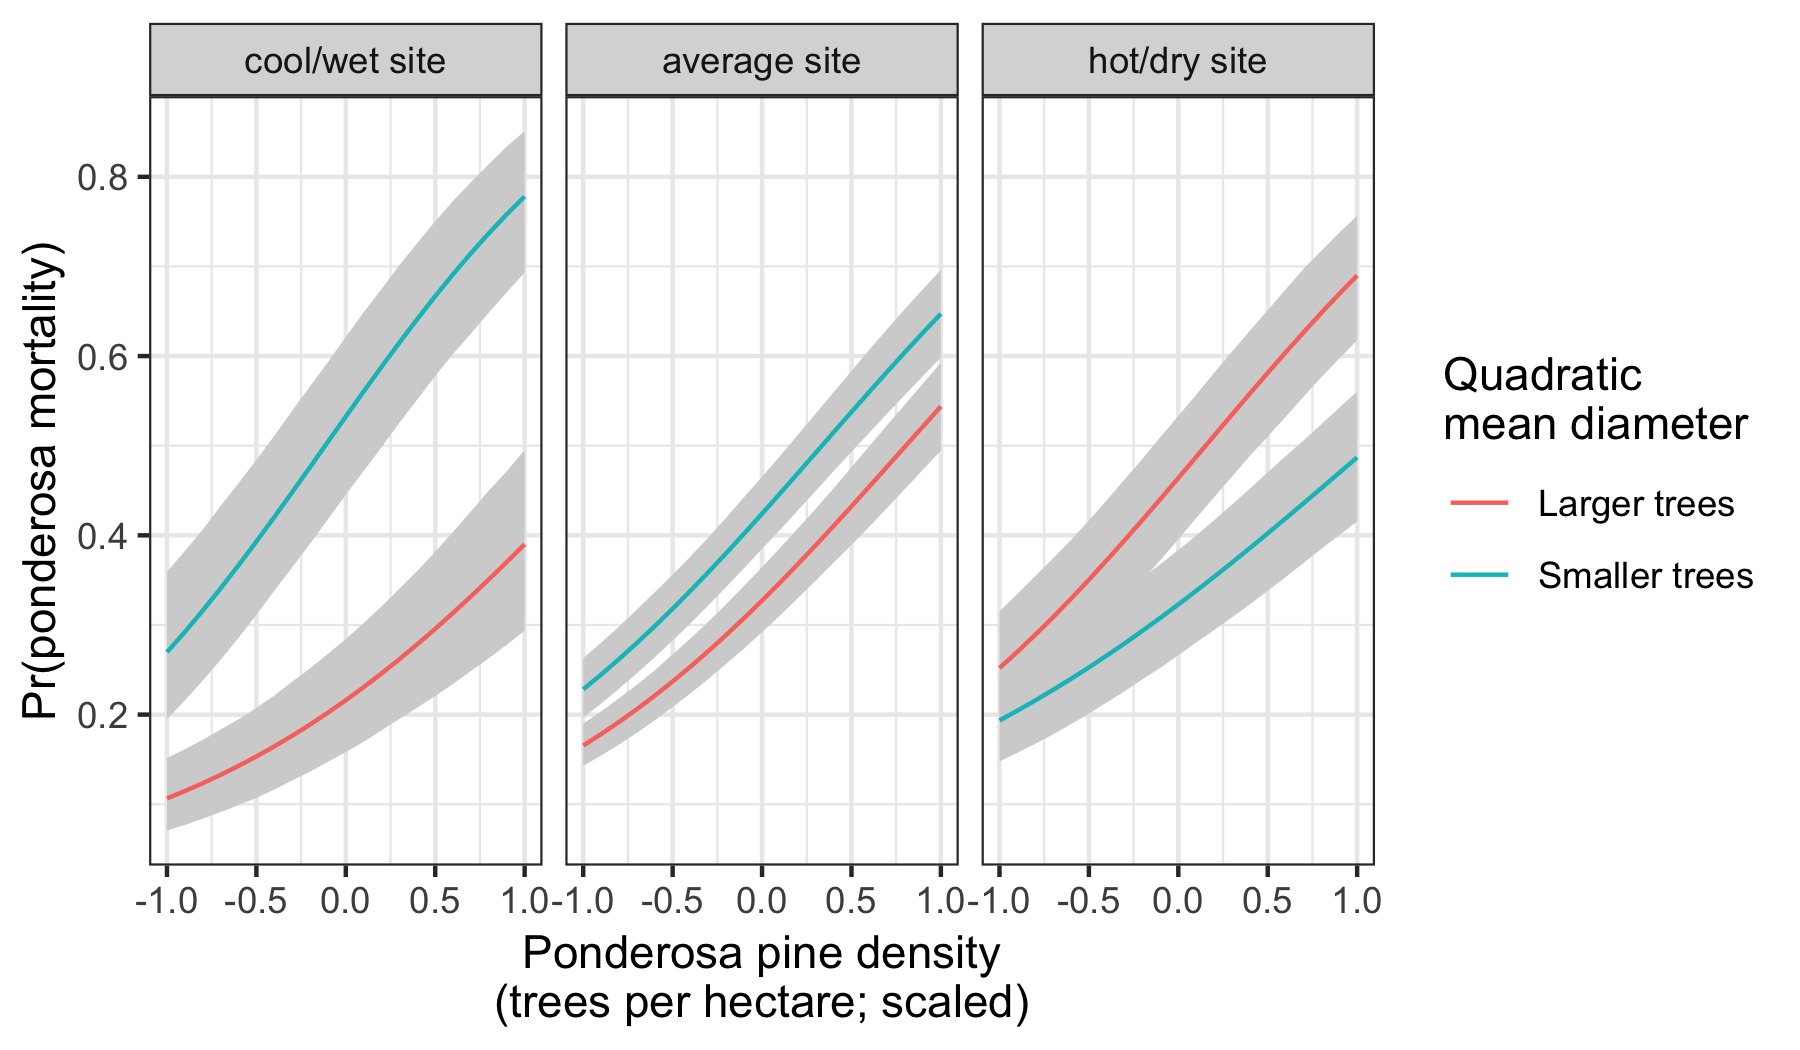
\includegraphics[width=6.00000in]{figure/chap02/pipo_tpha_qmd_cwd_interaction.png}
\caption{Line version of model results with 95\% credible intervals
showing primary influence of ponderosa pine structure on the probability
of ponderosa pine mortality, and the interaction across climatic water
deficit. The `larger trees' line represents the quadratic mean diameter
of ponderosa pine 0.7 standard deviations above the mean, and the
`smaller trees' line represents the quadratic mean diameter of ponderosa
pine 0.7 standard deviations below the mean.}
\end{figure}
\section{Discussion}\label{discussion-1}

We found that host tree density is a dominant driver of host mortality
during elevated levels of bark beetle activity, likely due to energy
costs associated with beetles navigating forests with many non-hosts
available. We also found that, even within a single forest insect/tree
species pairing, in the same extreme drought, and conditional upon high
levels of western pine beetle activity, host tree size may still
strongly affect insect-induced tree mortality in different ways
depending on background environmental conditions of water stress. We
suggest that this may indicate different stages of bark beetle
disturbance throughout the Sierra yellow pine/mixed-conifer system, with
``outbreak'' thresholds surpassed at the hottest, driest sites where
larger trees led to more likely host mortality, but not yet surpassed in
cooler, wetter sites, where smaller trees led to more likely host
mortality.

\subsection{Broad-scale environmental
condition}\label{broad-scale-environmental-condition}

We were surprised to only find a weakly positive main effect of climatic
water deficit on the probability of ponderosa mortality, though an
effect did materialize through its interaction with forest structure. We
did not measure tree water stress at an individual tree level as in
other recent work (Stephenson et al.
\protect\hyperlink{ref-stephenson2019}{2019}), and were instead treating
climatic water deficit as a general indicator of tree stress following
results of coarser-scale studies (Asner et al.
\protect\hyperlink{ref-asner2016}{2016}, Young et al.
\protect\hyperlink{ref-young2017}{2017}) which may have contributed to
our failure to detect a strong effect. Also, our entire study area
experienced the same extreme hot drought between 2012 and 2015 and the
variation of mortality explained by a main effect of climatic water
deficit may be dampened when most trees are experiencing a high degree
of water stress (Floyd et al. \protect\hyperlink{ref-floyd2009}{2009},
Fettig et al. \protect\hyperlink{ref-fettig2019}{2019}).

\subsection{\texorpdfstring{Strength of support for different ``density
increases mortality''
hypotheses}{Strength of support for different density increases mortality hypotheses}}\label{strength-of-support-for-different-density-increases-mortality-hypotheses}

The strongest effect on the probability of host mortality was the local
host density within each 20m x 20m cell. Host availability has been
shown to have a strong influence on the prevalence of host mortality
(Raffa and Berryman \protect\hyperlink{ref-raffa1987}{1987}). This can
arise as beetles require shorter flights to disperse to new hosts and
beetles are less likely to land on a non-host tree which imposes a
``sunk cost'' of energy expenditure in getting to that tree. Reduced
dispersal distances to host trees likely favors successful bark beetle
attacks, but we calibrated our aerial tree detection to
\textasciitilde{}400 m\textsuperscript{2} areas rather than to
individual tree locations so don't have the data precision to address
this hypothesis directly. Because we also found a strong negative effect
of overall tree density (host plus non-host) within each cell while
accounting for host density, we suspect that the positive association
between host density and host mortality might be driven by increasing
the frequency that western pine beetles land on their preferred host and
avoid expending energy flying to non-hosts. The negative relationship
that we detected between overall tree density and host mortality
corroborates findings from Fettig et al.
(\protect\hyperlink{ref-fettig2019}{2019}) and perhaps the ``sunk cost''
of landing on non-hosts explains those findings, though Fettig et al.
(\protect\hyperlink{ref-fettig2019}{2019}) didn't simultaneously model
the effect of host density. In general, Hayes et al.
(\protect\hyperlink{ref-hayes2009}{2009}) and Fettig et al.
(\protect\hyperlink{ref-fettig2019}{2019}) found that measures of host
availability explained less variation in mortality than measures of
overall tree density, but those conclusions were based on a response
variable of ``total number of dead host trees,'' rather than the number
of dead host trees conditional on the total number of host trees as in
our study (i.e., a binomial response).

Counter to our expectations, we found an overall negative effect of host
tree mean size on the probability of host mortality. Generally, smaller
trees are easier for western pine beetles to overwhelm in a mass attack
and are prime targets under normal levels of tree water stress. However,
larger trees are more nutritious and are therefore ideal targets if
local bark beetle density is high enough to successfully initiate mass
attack as can occur when many trees are under severe water stress (Bentz
et al. \protect\hyperlink{ref-bentz2010}{2010}). In the recent hot
drought, we expected that most trees would be under severe water stress,
setting the stage for increasing beetle density, successful mass
attacks, and targeting of larger trees. Larger average tree size in this
case would therefore lead to greater ponderosa pine mortality, as was
found in coincident ground plots (Fettig et al.
\protect\hyperlink{ref-fettig2019}{2019}) and other studies (Stephenson
et al. \protect\hyperlink{ref-stephenson2019}{2019}, Pile et al.
\protect\hyperlink{ref-pile2019}{2019}). One possible explanation for
our finding is that our observations represent the cumulative mortality
of trees during a multi-year drought event and its aftermath. Lower host
tree mean size led to a greater probability of host mortality earlier in
the drought (Pile et al. \protect\hyperlink{ref-pile2019}{2019}) and
that signal might have persisted even as mortality continued to
accumulate driven by other factors.

We did find a clear host tree size effect in its interaction with the
climatic water deficit. In hot, dry sites, larger average host size
increased the probability of host mortality while smaller host sizes
increased the probability of host mortality in cool, wet sites. This
suggests that the same bark beetle species was cueing into different
aspects of forest structure across the environmental gradient. This
represents an intraspecific version of the results of Stephenson et al.
(\protect\hyperlink{ref-stephenson2019}{2019}), who found that
insect-induced tree mortality in the same region during the same hot
drought were driven by different factors for different tree species. For
instance, Stephenson et al.
(\protect\hyperlink{ref-stephenson2019}{2019}) found that ponderosa pine
mortality was largely driven by host selection behavior of forest
insects, where larger more nutritious trees were specifically targeted
regardless of whether they exhibited signs of stress. In contrast,
Stephenson et al. (\protect\hyperlink{ref-stephenson2019}{2019}) found
that white fir mortality occurred predominantly in the slower growing,
smaller, stressed trees. In our study, we found that, even within a
single pairing of forest insect species and its host, the host tree size
affected host mortality differently depending on the site-level climatic
water deficit.

For aggressive bark beetles, massive tree mortality as observed from the
2012-2015 drought and its aftermath does not necessarily distinguish
``endemic'' from ``outbreak'' phases of bark beetle disturbance, which
is instead distinguished by the underlying driver of bark beetle host
selection behavior (Logan et al.
\protect\hyperlink{ref-logan1998}{1998}). ``Endemic'' phases are
distinguished by environmental determinism, when beetles select hosts
based on whether they are weakened in some way, often by environmental
conditions. ``Outbreak'' phases are distinguished by dynamic
determinism, when population dynamics reign-- when local beetle density
is high enough that intraspecific pheromone communication dominates host
selection, successful mass attacks are likely, and even large healthy
trees can be killed (White and Powell
\protect\hyperlink{ref-white1997}{1997}, Logan et al.
\protect\hyperlink{ref-logan1998}{1998}). Despite high local levels of
tree mortality across our study area (Fettig et al.
\protect\hyperlink{ref-fettig2019}{2019}), our results from surveying
the broader context surrounding coincident ground plots reveals
different effects of host tree size depending on the climatic water
deficit, and perhaps different stages of bark beetle disturbance across
the environmental gradient. This may help explain the especially high
host mortality in high host density, low host size cells that we
observed in cool/wet sites (Figure 2.13). The smaller trees would
presumably be nutritionally sub-optimal, and thus unexpected targets if
the western pine beetle were indeed in an ``outbreak'' phase at these
sites and able to attack even large, healthy trees. While trees were
likely water stressed across the whole study due to the extreme drought,
we expected generally less water stress in the cool/wet sites, and
generally higher water stress in the hot/dry sites (Asner et al.
\protect\hyperlink{ref-asner2016}{2016}, Young et al.
\protect\hyperlink{ref-young2017}{2017}). Thus, it is possible that the
observed mortality patterns across the Sierra Nevada during the
2012-2015 hot drought arose as synergistic alignment of environmental
conditions and complex forest structure enabled the western pine beetle
to cross thresholds of ``outbreak'' behavior in the hottest, driest
sites but such an alignment was not present in the cooler, wetter sites
(Raffa et al. \protect\hyperlink{ref-raffa2008}{2008}).

\subsection{Limitations and future
directions}\label{limitations-and-future-directions}

We have demonstrated that drones can be effective means of collecting
data at multiple, vastly different spatial scales to investigate a
single, multi-scale phenomenon-- from meters in between trees, to
hundreds of meters of elevation, to hundreds of thousands of meters of
latitude. However, some limitations remain but could perhaps be overcome
with further refinements in the use of this tool for forest ecology.
Most of these limitations arise from tree detection and classification
uncertainty, and thus it was imperative to work with field data for
calibration and uncertainty reporting.

The greatest limitation in our study arising from classification
uncertainty is in the assumption that all dead trees were ponderosa
pine. We estimate from coincident ground plots that this is true
approximately 73.4\% of the time. Because tree mortality response to
forest insects is species-specific, even with sympatric tree species
during the same hot drought (Stephenson et al.
\protect\hyperlink{ref-stephenson2019}{2019}), we cannot entirely rule
out that some of the mortality responses to complex forest structure
that we observed arose from these species-specific responses. The
overall community composition across our study area was not very
different (Fettig et al. \protect\hyperlink{ref-fettig2019}{2019}), so
we remain confident that the patterns we observed were driven primarily
by the dynamic between the western pine beetle and ponderosa pine.

Our ability to detect trees using the geometry of the dense point clouds
derived with the SfM was also limited. The horizontal accuracy of the
tree detection was better than the vertical accuracy, which may result
from a more significant error contribution by the ground-based
calculations of tree height compared to tree position relative to plot
center (Table 2.4). Both the horizontal and vertical accuracy would
likely improve with better SfM point clouds, which requires imagery with
more overlap. Frey et al. (\protect\hyperlink{ref-frey2018}{2018})
recently found that 95\% overlap was preferable for generating dense
point clouds, and we only achieved 91.6\% overlap with the X3 RGB camera
and 83.9\% overlap with the multispectral camera. While our live/dead
classification was fairly accurate (97.3\% on a withheld dataset), our
species classifier would likely benefit from better crown segmentation
because the pixel-level reflectance values within each crown are
averaged to characterize the ``spectral signature'' of each tree. With
better delineation of each tree crown, the mean value of pixels within
each tree crown will likely be more representative of that tree's
spectral signature. Better crown segmentation would most readily be
achieved through greater overlap in imagery. Finally, we anticipate that
computer vision and deep learning will prove helpful in overcoming some
of these detection and classification challenges (Gray et al.
\protect\hyperlink{ref-gray2019}{2019}).

\subsection{Conclusions}\label{conclusions-1}

Climate change adaptation strategies emphasize reducing tree densities
to restore forest resilience (North et al.
\protect\hyperlink{ref-north2015}{2015}, Young et al.
\protect\hyperlink{ref-young2017}{2017}), but understanding the optimal
complex forest structure that can enable dry western U.S. forests to
persist through disturbances such as insect attack will be vital for
predicting how California forests may respond to these interventions.
We've shown that drones can be a valuable tool for investigating how
this complexity in forest structure combines with environmental
conditions to shape forest insect disturbance.

Our results support conclusions of other researchers that management
interventions to reduce the severity of bark beetle disturbance will
benefit from generally reducing tree density (Young et al.
\protect\hyperlink{ref-young2017}{2017}). However, in addition, our
study suggests that outcomes will depend on whether the disturbance
dynamic has crossed endemic to outbreak feedback thresholds (Raffa et
al. \protect\hyperlink{ref-raffa2008}{2008}), which may be predicted by
recent advances in disturbance forecasting (Preisler et al.
\protect\hyperlink{ref-preisler2017}{2017}).

\section{Acknowledgements}\label{acknowledgements-1}

We gratefully acknowledge funding from the US Forest Service Western
Wildlands Environmental Threat Assessment Center (WWETAC) as well as
Connie Millar for comments and guidance during the development of this
project.

\chapter{Initial wildfire suppression efforts select for more extreme
fuel and climate burning conditions in Sierra Nevada
forests}\label{initial-wildfire-suppression-efforts-select-for-more-extreme-fuel-and-climate-burning-conditions-in-sierra-nevada-forests}

Michael J. Koontz\textsuperscript{1,2,*}, Zachary L.
Steel\textsuperscript{3}, Andrew M. Latimer\textsuperscript{1,2},
Malcolm P. North\textsuperscript{1,2,4}

\textsuperscript{1}Graduate Group in Ecology, University of California,
Davis, CA, USA\\
\textsuperscript{2}Department of Plant Sciences, University of
California, Davis, CA, USA\\
\textsuperscript{3}Department of Environmental Science and Policy,
University of California, Berkeley, CA, USA\\
\textsuperscript{4}USDA Forest Service, Pacific Southwest Research
Station, Mammoth Lakes, CA, USA

\section{Abstract}\label{abstract-2}

Typical fire effects in dry western pine and mixed-conifer forests are
dominated by large wildfires, and potential fire effects of rapidly
suppressed fires are never realized. Milder fuel and weather conditions
facilitate suppression when fires are still small, and thus most
extensive fire effects in forest landscapes occur during more extreme
conditions. This amounts to a selection pressure on burning conditions
that may lead to a selection bias in average fire effects. We formalize
this selection framework and measure its influence on correlated,
multivariate burning conditions of fuel and climate using the
evolutionary ecology concept of phenotypic selection. Using a new
dataset that includes smaller fires (\textgreater{}4ha), we examine fire
``survivorship'' to initial attack suppression efforts as a fitness
metric. Our analysis found that initial containment efforts select for
fires burning in more homogeneous fuel conditions and during
hotter/drier conditions. Fire effects on western forest conditions arise
from a complex social-ecological system, with management decision-making
having a strong ability to influence outcomes. We show a strong
selection pressure on burning conditions imposed by management, and
encourage further dismantling of barriers to applying this selection for
resource benefit, such as by expanding implementation of wildfire use
fires where natural ignitions are allowed to burn under moderate
conditions.

\section{Introduction}\label{introduction-2}

A legacy of fire suppression is an oft-cited root cause underpinning the
increasing size and severity of wildfires in the dry western U.S. pine
and mixed-conifer forests (Miller and Thode
\protect\hyperlink{ref-miller2007}{2007}, Calkin et al.
\protect\hyperlink{ref-calkin2015}{2015}, Safford and Stevens
\protect\hyperlink{ref-safford2017}{2017}). While most of this ecosystem
would experience frequent, low- to moderate-severity wildfire every 8 to
15 years in the several centuries prior to Euroamerican settlement,
suppression management has largely eliminated fire effects from much of
western dry forested land in the past 100 years (Steel et al.
\protect\hyperlink{ref-steel2015}{2015}, Safford and Stevens
\protect\hyperlink{ref-safford2017}{2017}, Miller and Safford
\protect\hyperlink{ref-miller2017}{2017}). A lack of frequent fire has
led to densification of these forests, which increases fuel loading and
homogenizes forest structure (Fulé et al.
\protect\hyperlink{ref-fule1997}{1997}, Veblen et al.
\protect\hyperlink{ref-veblen2000}{2000}, Keane et al.
\protect\hyperlink{ref-keane2002a}{2002}, Collins et al.
\protect\hyperlink{ref-collins2016}{2016}, Stephens et al.
\protect\hyperlink{ref-stephens2018}{2018}). Synergistic alignment of
these extreme fuel conditions with earlier snow melt, longer fire
seasons, and hotter droughts (aka ``climate change droughts'')
(Westerling \protect\hyperlink{ref-westerling2006}{2006},
\protect\hyperlink{ref-westerling2016}{2016}, Abatzoglou and Kolden
\protect\hyperlink{ref-abatzoglou2013a}{2013}, Abatzoglou and Williams
\protect\hyperlink{ref-abatzoglou2016}{2016}) increases the probability
that fires will generate self-propagating behavior (Coen et al.
\protect\hyperlink{ref-coen2018}{2018}) and kill all (or nearly all)
overstory vegetation (Koontz et al.
\protect\hyperlink{ref-koontz2019a}{2019}\protect\hyperlink{ref-koontz2019a}{b})
in large, contiguous patches of mortality (Stevens et al.
\protect\hyperlink{ref-stevens2017}{2017}). Most dry western conifer
forests are ill-adapted to regenerate in the centers of these large
patches, which are far from seed sources (Welch et al.
\protect\hyperlink{ref-welch2016}{2016}, Stevens-Rumann et al.
\protect\hyperlink{ref-stevens-rumann2018}{2018}). Thus the modern trend
of atypically large, contiguously stand-replacing fires in this system
compromises forest resilience and increases the potential for long-term
shifts in vegetation type to shrub- or grasslands (North et al.
\protect\hyperlink{ref-north2009a}{2009}, Millar and Stephenson
\protect\hyperlink{ref-millar2015}{2015}, Stevens et al.
\protect\hyperlink{ref-stevens2017}{2017}).

Ongoing fire suppression also strongly influences fire effects. Fire
suppression generally is very effective at its immediate goal of
extinguishing fires. Between 1970 and 2002, 97 to 99\% of fires burning
on U.S. Forest Service land were contained before they reached 120
hectares in size (Calkin et al.
\protect\hyperlink{ref-calkin2005}{2005},
\protect\hyperlink{ref-calkin2015}{2015}). The ``10 a.m. policy'', which
dictated that fires should be put out before 10 a.m. on the day
following their discovery, has been modified since its establishment as
firefighting policy in the 1930's but its aggressive spirit persists in
today's modern firefighting apparatus (Dale
\protect\hyperlink{ref-dale2006}{2006}, Johnson et al.
\protect\hyperlink{ref-johnson2009}{2009}). Mild weather and fuel
conditions facilitate early suppression efforts (Calkin et al.
\protect\hyperlink{ref-calkin2015}{2015}, Abatzoglou et al.
\protect\hyperlink{ref-abatzoglou2018a}{2018}), and the fires that
escape initial attack and grow large are often assumed to have grown to
these sizes because they were burning under more extreme conditions
(Calkin et al. \protect\hyperlink{ref-calkin2014}{2014}).

While the vast majority of fires are managed for suppression in the
western U.S. (Calkin et al. \protect\hyperlink{ref-calkin2015}{2015}), a
small number of natural ignitions are allowed to burn under moderate
conditions as ``wildland fire use'' (WFU) fires in recognition of the
benefit that fire has to forest resources (Davis
\protect\hyperlink{ref-davis1979}{1979}). WFU fire effects tend to fall
within the natural range of variation for western pine and mixed-conifer
systems (Meyer \protect\hyperlink{ref-meyer2015}{2015}, Walker et al.
\protect\hyperlink{ref-walker2018}{2018}). Though many studies recommend
WFU fires as a means to restore forest resilience (Mallek et al.
\protect\hyperlink{ref-mallek2013}{2013}, Meyer
\protect\hyperlink{ref-meyer2015}{2015}, North et al.
\protect\hyperlink{ref-north2015}{2015}, Collins et al.
\protect\hyperlink{ref-collins2017}{2017}, Stevens et al.
\protect\hyperlink{ref-stevens2017}{2017}), barriers remain to their
more widespread adoption (Doane et al.
\protect\hyperlink{ref-doane2006}{2006}).

The same mild fuel and weather conditions that contribute to beneficial
outcomes of WFU fires contribute to early success of suppression
efforts. Fire effects that may have arisen from fires that succumb to
early suppression efforts never materialize. Instead, fire effects from
suppression fires in this ecosystem are dominated by large fires, which
account for approximately 97.5\% of total burned area, exhibit fire
effects that increase the likelihood of state change, and likely burn
under the more extreme fuel and weather conditions that hindered early
suppression efforts (Calkin et al.
\protect\hyperlink{ref-calkin2005}{2005}). Thus, the general short-term
success of fire suppression policy paired with its long-term cumulative
effect has led to a management paradox with respect to forest management
aiming to restore resilience: \emph{we shouldn't put out the fires that
we can, and we can't put out the fires that we should}.

Wildfire suppression management has shifted the distribution of fire
behavior, and therefore the distribution of fire effects, to be more
extreme (Calkin et al. \protect\hyperlink{ref-calkin2015}{2015}). Here,
we introduce the evolutionary ecology concept of ``phenotypic
selection'' as a formal framework for measuring the magnitude of this
distributional shift-- the selection by suppression. We use a new
dataset of fire severity compiled for yellow pine/mixed-conifer forests
(Koontz et al.
\protect\hyperlink{ref-koontz2019}{2019}\protect\hyperlink{ref-koontz2019}{a})
to quantify the strength of ``selection'' on wildfire burning conditions
(regional climate, wind speed, vegetation density, vegetation
continuity) imposed by initial attack suppression efforts. In
particular, we examine the following questions:
\begin{enumerate}
\def\labelenumi{\arabic{enumi}.}
\item
  How do initial burning conditions (regional climate, vegetation
  density, vegetation continuity) differ between suppression fires that
  are successfully contained by initial attack and those that escape
  containment efforts?
\item
  What are the consequences of these varying conditions for wildfire
  effects (burn duration, fire event size, severity configurations)?
\item
  How might this selection be biasing our understanding of fire effects
  arising from suppression and wildfire use fires?
\end{enumerate}
\section{Methods}\label{methods-1}

\subsection{Study system}\label{study-system-2}

The Sierra Nevada yellow pine/mixed-conifer (hereafter Sierra YPMC) is a
disturbance-prone forest system in the Sierra Nevada mountain range of
California, U.S.A. It spans the full 628 kilometer latitudinal length of
the Sierra Nevada, and 2,500 meters of elevation (300 meters to 2800
meters), primarily on the western slope of the mountain range (Safford
and Stevens \protect\hyperlink{ref-safford2017}{2017}). The forest is
dominated by ponderosa pine (\emph{Pinus ponderosa}), sugar pine
(\emph{Pinus lambertiana}), white fir (\emph{Abies concolor}), and
incense cedar (\emph{Calocedrus decurrens}) in varying mixes. Prior to
Euroamerican settlement, the ecosystem experienced frequent, low- to
moderate-severity wildfire every 8 to 15 years on average (Steel et al.
\protect\hyperlink{ref-steel2015}{2015}, Safford and Stevens
\protect\hyperlink{ref-safford2017}{2017}), which consumed surface fuels
but generally had minimal effects on large, established trees. This fire
regime generated heterogeneous horizontal forest structure, with groups
of relatively even-aged trees having interlocking crowns, individual
trees with distinct crowns, and variably-sized gaps between these tree
clump and individual tree structural features (Lydersen et al.
\protect\hyperlink{ref-lydersen2013}{2013}). A century of fire
suppression has led to infill of these gaps, homogenizing the horizontal
forest structure, increasing vertical continuity of fuels, and
compromising forest resilience in an era of climate change-induced
hotter droughts (North et al. \protect\hyperlink{ref-north2009a}{2009},
Millar and Stephenson \protect\hyperlink{ref-millar2015}{2015}, Collins
et al. \protect\hyperlink{ref-collins2016}{2016}).

For our study, we compiled the Sierra YPMC type using the U.S. Forest
Service Fire Return Interval Departure (FRID) dataset and included ``dry
mixed-conifer'', ``moist mixed-conifer'', and ``yellow pine'' vegetation
types following Steel et al. (\protect\hyperlink{ref-steel2018}{2018})
and Koontz et al.
(\protect\hyperlink{ref-koontz2019a}{2019}\protect\hyperlink{ref-koontz2019a}{b}).
These classifications represent ``potential vegetation'' given the
climate of the area, such that there is no influence of recent
disturbance events (Harvey et al.
\protect\hyperlink{ref-harvey2016b}{2016}, Steel et al.
\protect\hyperlink{ref-steel2018}{2018}, Koontz et al.
\protect\hyperlink{ref-koontz2019a}{2019}\protect\hyperlink{ref-koontz2019a}{b}).

\subsection{Context of Sierra YPMC
wildfire}\label{context-of-sierra-ypmc-wildfire}

To describe the modern context of wildfire activity in the Sierra Nevada
yellow pine/mixed-conifer system, we used geospatial records contained
in Short (\protect\hyperlink{ref-short2017}{2017}) (U.S. Forest Service
Fire Program Analysis Fire Occurrence Database; FPAFOD), the most
comprehensive database of wildfire occurrence for the United States
representing 1.88 million wildfire records from 1992 to 2015.

The FPAFOD contains point locations for the centroids of each fire's
footprint, rather than the perimeter of each fire as in some other
databases (Eidenshink et al.
\protect\hyperlink{ref-eidenshink2007}{2007}). We spatially subsetted
the FOD data to fire events whose centroids occurred within the Sierra
Nevada mountain range, as defined by the Jepson geographic subdivisions
(north, central, and south Sierra Nevada Foothills and High Sierra
Nevada, as well as the Tehachapi Mountain Area) (JepsonFloraProject
\protect\hyperlink{ref-jepsonfloraproject2016}{2016}). For each fire
record, we approximated its footprint by creating a circular buffer
around the centroid with an area equivalent to the reported area of the
fire. Using this footprint approximation, we calculated the proportion
of area that intersected with our compilation of Sierra YPMC from the
FRID dataset. We retained all fires with greater than zero area of the
approximate footprint covering the Sierra YPMC extent. We calculated
burn duration as the number of days between the containment date and the
alarm date, and retained all fires with a burn duration of greater than
0 and less than 364 days to eliminate likely errors in reporting of
alarm and containment dates (e.g., switched alarm date and containment
date creating negative burn duration, typo in containment year creates a
5+ year burn duration).

\subsection{Measuring wildfire
severity}\label{measuring-wildfire-severity}

The CalFire Fire Resource and Protection Program (FRAP;
\url{http://frap.fire.ca.gov/}) maintains the most comprehensive Dataset
of wildfire perimeters in the state of California, including attribute
data for each fire such as its discovery date, its containment date, and
the management objective. The management objective represents the
approach taken by the management unit overseeing the wildfire-- either
``suppression'', with a goal of extinguishing the fire, or ``wildland
fire use'', with a goal of allowing the fire to burn to benefit forest
resources so long as it didn't threaten lives or property (Meyer
\protect\hyperlink{ref-meyer2015}{2015}). This dichotomy is somewhat
simplistic, as each wildfire can be managed for multiple objectives, but
it is a generally useful framework for understanding the primary
management goal (Meyer \protect\hyperlink{ref-meyer2015}{2015}). This
dataset contains all fires \textgreater{}4 hectares (and a
non-comprehensive set of fires \textless{}4 hectares), and thus has
greater representation of fire events, particularly events of smaller
size, compared to other wildfire events datasets, though it lacks
severity information. For instance, the Monitoring Trends in Burn
Severity (MTBS) database only contains wildfires in the western U.S.
that are larger than 400 hectares (Eidenshink et al.
\protect\hyperlink{ref-eidenshink2007}{2007}) and the U.S. Forest
Service Region 5 geospatial database contains wildfires in the Sierra
Nevada that are larger than 80 hectares (Steel et al.
\protect\hyperlink{ref-steel2018}{2018}), though both of these datasets
contain information on wildfire severity.

To assess the severity of these smaller fires, Koontz et al.
(\protect\hyperlink{ref-koontz2019}{2019}\protect\hyperlink{ref-koontz2019}{a})
used the expanded FRAP dataset of over 1,000 wildfire perimeters to
calculate wildfire severity and calibrate satellite-derived measures
using ground-based overstory composite burn index (CBI) (Koontz et al.
\protect\hyperlink{ref-koontz2019a}{2019}\protect\hyperlink{ref-koontz2019a}{b}),
which is an integrated measure of the effect of a wildfire on the forest
overstory one year after the burn (Key and Benson
\protect\hyperlink{ref-key2006}{2006}). CBI correlates well with direct
measures of fire impact to vegetation in Sierra YPMC, such as percent of
overstory mortality (Miller and Thode
\protect\hyperlink{ref-miller2007}{2007}). Thresholds of wildfire
severity (unchanged, low, moderate, and high) calibrated to the full
dataset (Koontz et al.
\protect\hyperlink{ref-koontz2019a}{2019}\protect\hyperlink{ref-koontz2019a}{b})
were imposed on each fire and then contiguous pixels of each category
were vectorized into polygons to form patches of each severity category.
We subsetted this FRAP-derived dataset of fire severity to 622 that
burned in majority yellow pine/mixed-conifer forest (547 suppression
fires; 75 WFU fires).

\subsection{Burning conditions per fire
event}\label{burning-conditions-per-fire-event}

In addition to mapping wildfire severity across each fire in the FRAP
perimeter database, Koontz et al.
(\protect\hyperlink{ref-koontz2019a}{2019}\protect\hyperlink{ref-koontz2019a}{b})
also calculated fuel and regional climate variables within the burn
perimeter. The prefire Normalized Difference Vegetation Index (NDVI;
Rouse et al. (\protect\hyperlink{ref-rouse1973}{1973}){]}) was found to
correlate strongly with local wildfire severity, as was the standard
deviation of NDVI within the 90m x 90m window surrounding each pixel,
which represents a measure of horizontal forest structure and fuel
continuity (Koontz et al.
\protect\hyperlink{ref-koontz2019a}{2019}\protect\hyperlink{ref-koontz2019a}{b}).
The gridMET product (Abatzoglou
\protect\hyperlink{ref-abatzoglou2013}{2013}) was used to calculate the
energy release component, a modeled estimate of expected fire behavior
in conifer forest, for the 3 days prior to each fire's discovery date as
well as the wind speed for the first three days of the fire. The gridMET
product has a daily temporal resolution and a 4 kilometer spatial
resolution, so our climate variables capture regional conditions over
time periods of several days, but not very local weather events that
might occur over the span of hours. Each of these variables has a strong
impact on wildfire behavior at macroscales (Abatzoglou and Kolden
\protect\hyperlink{ref-abatzoglou2013a}{2013}).

For this study, we assigned prefire burning conditions for each fire as
the mean fuel (prefire NDVI, prefire standard deviation of NDVI within
90m x 90m moving windows) and regional climate (energy release component
for 3 days prior to the fire, wind speed for first 3 days of the fire)
values within each fire perimeter.

For each fire, we calculated the total number of fires burning on that
fire's alarm date, the proportion of area represented by each severity
category, as well as the maximum patch size of each severity category.
Finally, we calculated the stand replacing decay coefficient (SDC)
(Collins et al. \protect\hyperlink{ref-collins2017}{2017}, Stevens et
al. \protect\hyperlink{ref-stevens2017}{2017}), a single metric that
integrates high severity patch size and shape such that a lower SDC
corresponds to a larger, more circular high severity patches with
effectively more area within those patches far from the patch edges
(i.e., beyond likely seed dispersal estimated for yellow
pine/mixed-conifer species).

\subsection{\texorpdfstring{Designating ``survivorship'' of suppression
fires}{Designating survivorship of suppression fires}}\label{designating-survivorship-of-suppression-fires}

For each wildfire in the Koontz et al.
(\protect\hyperlink{ref-koontz2019a}{2019}\protect\hyperlink{ref-koontz2019a}{b})
dataset with a suppression management objective, we determined whether
it ``survived'' initial attack by whether its burn duration (discovery
date subtracted from the containment date) was greater than 1 day.
Following Abatzoglou et al.
(\protect\hyperlink{ref-abatzoglou2018a}{2018}), we assumed that fires
under a suppression management objective that burned for more than one
day would require different firefighting tactics than direct attack and
thus represented a reconfiguration of firefighting personnel and
resource allocation.

\subsection{Quantifying the selection effect of fire
suppression}\label{quantifying-the-selection-effect-of-fire-suppression}

We treated the prefire fuel (prefire NDVI, heterogeneity of NDVI) and
climate conditions (prefire energy release component, early fire wind
speed) as wildfire ``phenotypes'' having some distribution, and used
logistic regression to measure the extent to which wildfire suppression
``selected'' for particular burning condition phenotypes using the
survivorship of each fire from initial attack as a binary response
fitness metric in an evolutionary ecology framework (Lande and Arnold
\protect\hyperlink{ref-lande1983}{1983}, Janzen and Stern
\protect\hyperlink{ref-janzen1998}{1998}).

\subsection{Implications of selection by
suppression}\label{implications-of-selection-by-suppression}

We graphically compare fire effects (event size, stand replacing decay
coefficient, proportion high severity) of suppression fires to those of
wildfire use (WFU) fires to draw inferences about how the ``lost
contribution'' of fires that succumbed to early containment may have
influenced fire effects.

\subsection{Software and data
availability}\label{software-and-data-availability-1}

Our selection model was fit using the \texttt{brms} (Bürkner
\protect\hyperlink{ref-burkner2017}{2017}) package in \texttt{R} (R Core
Team \protect\hyperlink{ref-rcoreteam2018}{2018}). Our workflow greatly
benefited from the \texttt{tidyverse} group of packages (Wickham
\protect\hyperlink{ref-wickham2017}{2017}), and we manipulated spatial
data using the following \texttt{R} packages: \texttt{sf} (Pebesma
\protect\hyperlink{ref-pebesma2018}{2018}), \texttt{raster} (Hijmans et
al. \protect\hyperlink{ref-hijmans2019}{2019}), \texttt{velox} (Hunziker
\protect\hyperlink{ref-hunziker2017}{2017}), \texttt{stars} (Pebesma
\protect\hyperlink{ref-pebesma2019b}{2019}\protect\hyperlink{ref-pebesma2019b}{a}),
\texttt{lwgeom} (Pebesma
\protect\hyperlink{ref-pebesma2019a}{2019}\protect\hyperlink{ref-pebesma2019a}{b}),
\texttt{fasterize} (Ross \protect\hyperlink{ref-ross2018}{2018}), and
\texttt{APfun} (Plowright
\protect\hyperlink{ref-plowright2018a}{2018}\protect\hyperlink{ref-plowright2018a}{a}).

The original severity dataset created by (Koontz et al.
\protect\hyperlink{ref-koontz2019}{2019}\protect\hyperlink{ref-koontz2019}{a})
can be found on the Open Science Framework
(\url{https://osf.io/ke4qj/}). The data and code for this study can also
be found on the Open Science Framework.

\section{Results}\label{results-2}

\subsection{Fire event size and burn duration context of Sierra YPMC
wildfire}\label{fire-event-size-and-burn-duration-context-of-sierra-ypmc-wildfire}

We found that 16219 fire events burned at least partially in Sierra
Nevada yellow pine/mixed-conifer between 1992 and 2015 covering 2.19
million total hectares and 1.18 million hectares within this forest
type. A total of 14873 fires burned in greater than 50\% Sierra yellow
pine/mixed-conifer in the same period. The vast majority of these fire
events were very small. Comparing the distribution of fire sizes in this
system between 1992 and 2015 to relevant reference sizes:
\begin{itemize}
\tightlist
\item
  61.46\% of fires were smaller than 0.09 hectares-- the size of a
  single pixel from Landsat which is a USGS satellite product often used
  to measure fire effects by comparing imagery just before the fire to
  imagery one year after the fire (Miller and Thode
  \protect\hyperlink{ref-miller2007}{2007}).
\item
  98.87\% of fires were smaller than 400 hectares-- the minimum fire
  size for inclusion in the MTBS dataset for the western U.S.
  (Eidenshink et al. \protect\hyperlink{ref-eidenshink2007}{2007}),
  meaning that MTBS would include approximately 1.13\% of fires in this
  system.
\item
  97.93\% of fires were smaller than 80 hectares-- the minimum fire size
  for inclusion in the USFS Region 5 geospatial dataset (Steel et al.
  \protect\hyperlink{ref-steel2018}{2018}), meaning that the USFS Region
  5 data accounts for approximately 2.07\% of fires in this system.
\item
  94.88\% of fires were smaller than 4 hectares-- the minimum fire size
  for inclusion in the CalFire FRAP fire perimeter dataset which was
  used to derive the Koontz et al.
  (\protect\hyperlink{ref-koontz2019}{2019}\protect\hyperlink{ref-koontz2019}{a})
  severity dataset. Thus, the Koontz et al.
  (\protect\hyperlink{ref-koontz2019}{2019}\protect\hyperlink{ref-koontz2019}{a})
  dataset includes approximately 5.12\% of fires in this system during
  its time span of 1984 to 2017.
\end{itemize}
\subsection{Context of suppression fires compared to wildfire use (WFU)
fires}\label{context-of-suppression-fires-compared-to-wildfire-use-wfu-fires}

There is a clear multimodality in the distribution of suppression fire
event size while wildfire use fire event sizes are lognormally
distributed (Figure 3.1). Under a suppression management objective, most
fires are successfully contained at relatively small sizes while WFU
fires are larger on average. This effect is obscured when comparing
median fire sizes between management objectives using just larger fires
(Table 3.1).

Median fire size of all suppression fires is much lower than the median
fire size of WFU fires, owing to the highly successful early suppression
efforts (Table 3.1). This size difference becomes less apparent as the
minimum fire size in the dataset is increased, as is the case for fire
effects datasets that focus on tracking larger fire events (e.g., U.S.
Forest Service Region 5 GIS dataset with a minimum fire size of 80 ha or
MTBS with a minimum fire size of 400 ha in the western U.S (Table 3.1).
The size difference is likely to be even more dramatic than what can be
seen in the FRAP-derived Koontz et al.
(\protect\hyperlink{ref-koontz2019a}{2019}\protect\hyperlink{ref-koontz2019a}{b})
dataset with its comprehensive coverage of fire greater than 4 ha (and
some additional fires smaller than this threshold), as nearly 95\% of
wildfires in the Sierra yellow pine/mixed-conifer region remain even
smaller than 4 ha.
\begin{longtable}[]{@{}ccccc@{}}
\caption{Comparison of fire event sizes by management objective for
fires burning in majority yellow pine/mixed-conifer in the Sierra Nevada
between 1984 and 2017.}\tabularnewline
\toprule
\begin{minipage}[b]{0.11\columnwidth}\centering\strut
Management objective\strut
\end{minipage} & \begin{minipage}[b]{0.19\columnwidth}\centering\strut
Median fire size (ha) All FRAP fires\strut
\end{minipage} & \begin{minipage}[b]{0.19\columnwidth}\centering\strut
Median fire size (ha) Fires \textgreater{} 4ha\strut
\end{minipage} & \begin{minipage}[b]{0.19\columnwidth}\centering\strut
Median fire size (ha) Fires \textgreater{} 80ha\strut
\end{minipage} & \begin{minipage}[b]{0.19\columnwidth}\centering\strut
Median fire size (ha) Fires \textgreater{} 400ha\strut
\end{minipage}\tabularnewline
\midrule
\endfirsthead
\toprule
\begin{minipage}[b]{0.11\columnwidth}\centering\strut
Management objective\strut
\end{minipage} & \begin{minipage}[b]{0.19\columnwidth}\centering\strut
Median fire size (ha) All FRAP fires\strut
\end{minipage} & \begin{minipage}[b]{0.19\columnwidth}\centering\strut
Median fire size (ha) Fires \textgreater{} 4ha\strut
\end{minipage} & \begin{minipage}[b]{0.19\columnwidth}\centering\strut
Median fire size (ha) Fires \textgreater{} 80ha\strut
\end{minipage} & \begin{minipage}[b]{0.19\columnwidth}\centering\strut
Median fire size (ha) Fires \textgreater{} 400ha\strut
\end{minipage}\tabularnewline
\midrule
\endhead
\begin{minipage}[t]{0.11\columnwidth}\centering\strut
suppression\strut
\end{minipage} & \begin{minipage}[t]{0.19\columnwidth}\centering\strut
16.77\strut
\end{minipage} & \begin{minipage}[t]{0.19\columnwidth}\centering\strut
29.13\strut
\end{minipage} & \begin{minipage}[t]{0.19\columnwidth}\centering\strut
582\strut
\end{minipage} & \begin{minipage}[t]{0.19\columnwidth}\centering\strut
1459\strut
\end{minipage}\tabularnewline
\begin{minipage}[t]{0.11\columnwidth}\centering\strut
wfu\strut
\end{minipage} & \begin{minipage}[t]{0.19\columnwidth}\centering\strut
193.1\strut
\end{minipage} & \begin{minipage}[t]{0.19\columnwidth}\centering\strut
205.4\strut
\end{minipage} & \begin{minipage}[t]{0.19\columnwidth}\centering\strut
506.7\strut
\end{minipage} & \begin{minipage}[t]{0.19\columnwidth}\centering\strut
866.5\strut
\end{minipage}\tabularnewline
\bottomrule
\end{longtable}
\begin{figure}
\centering
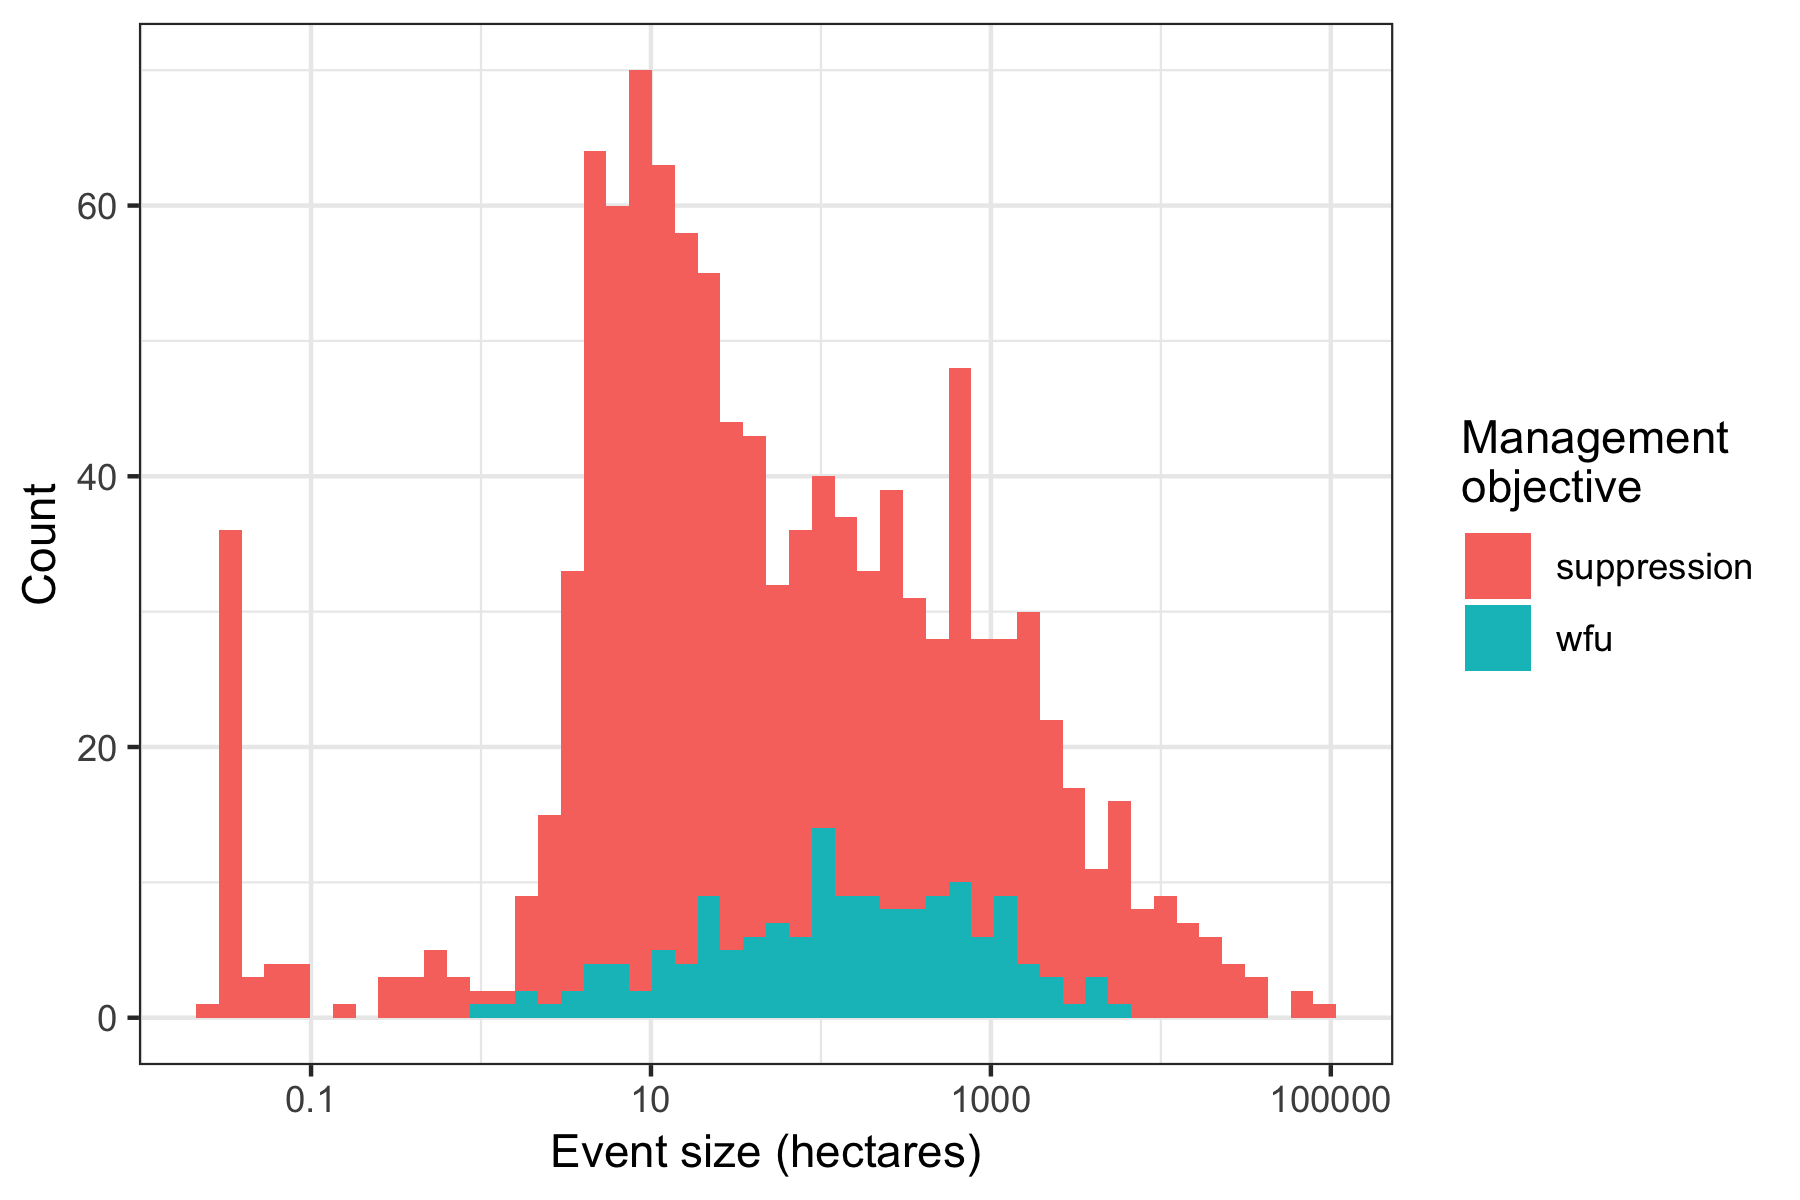
\includegraphics[width=6.00000in]{figure/chap03/fire-size-histogram-by-management-objective.png}
\caption{Distribution of log fire event size by management objective.
While wildfire use fires exhibit a lognormal distribution in size,
suppression fires exhibit clear multimodality with many fires
extinguished when they are very small.}
\end{figure}
\subsection{Selection by suppression}\label{selection-by-suppression}

We found a sizable effect of phenotypic selection of initial attack
suppression on the heterogeneity of NDVI and prefire energy release
component. Wildfires that survived initial attack were more likely to be
burning in more extreme, homogeneous fuels (lower heterogeneity of NDVI)
and in more extreme, hotter/drier climate conditions (higher energy
release component) compared to wildfires that succumbed to the initial
attack. We detected no selection pressure on prefire vegetation density
as measured by NDVI or wind speed during the first three days of the
fire (Figure 3.2; Figure 3.3).
\begin{figure}
\centering
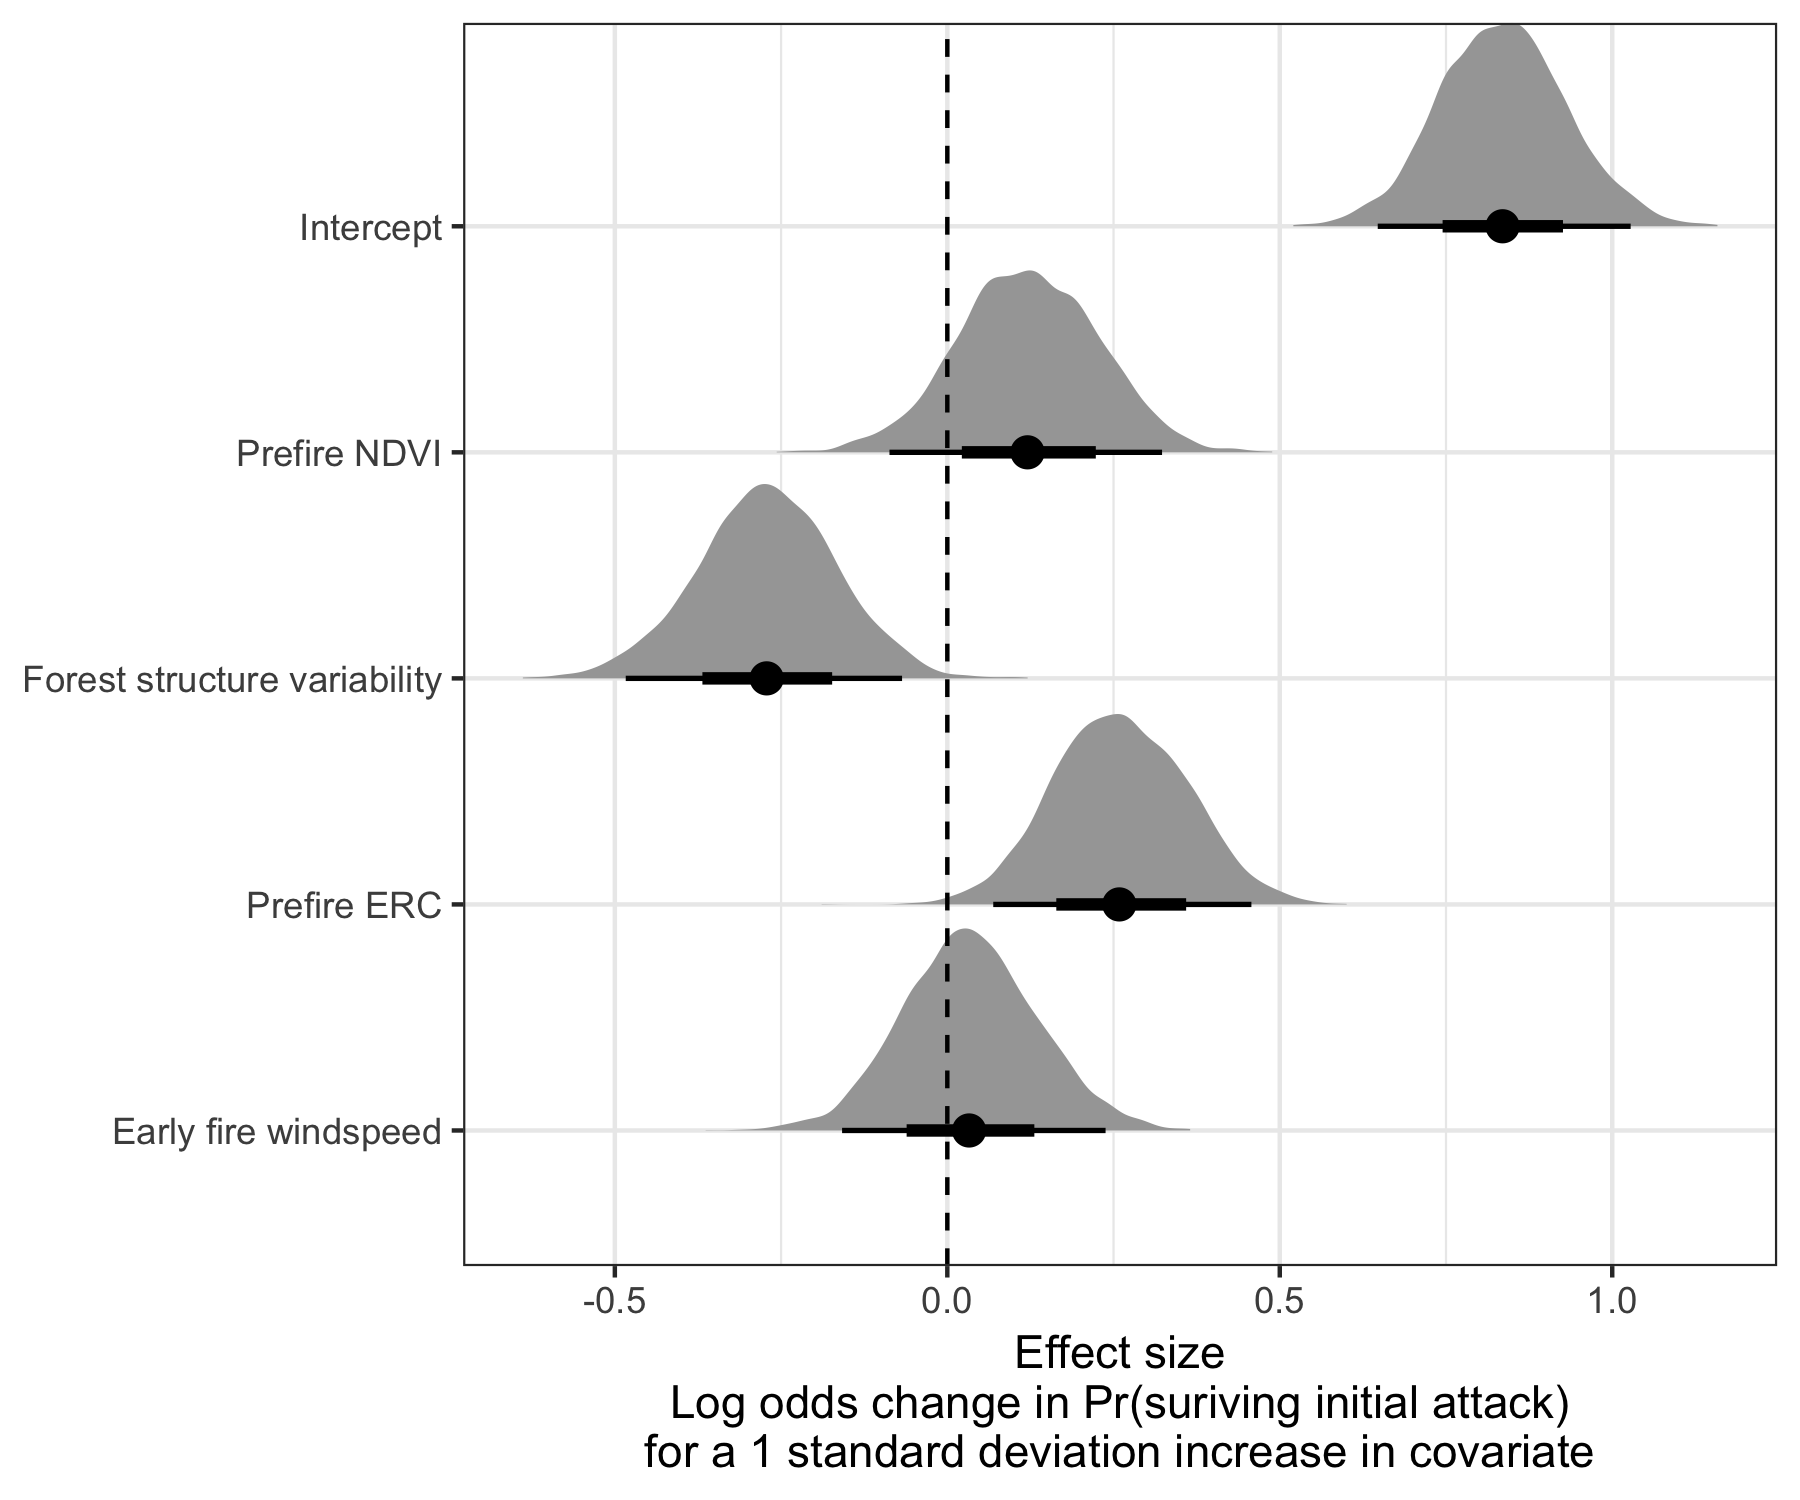
\includegraphics[width=6.00000in]{figure/chap03/selection-by-suppression-halfeye-simple.png}
\caption{Halfeye plot showing posterior distributions of coefficient
estimates for model predicting the probability of wildfire survivorship
in the first 48 hours of initial attack. The effect sizes are
proportional to the `strength of selection' of initial attack on the
burning conditions of wildfire. Credible intervals are shown below each
probability density function with the point representing the mean, the
dark line representing the 66\% credible interval, and the light line
representing the 95\% credible interval. The dotted line shows an effect
size of zero.}
\end{figure}
\begin{figure}
\centering
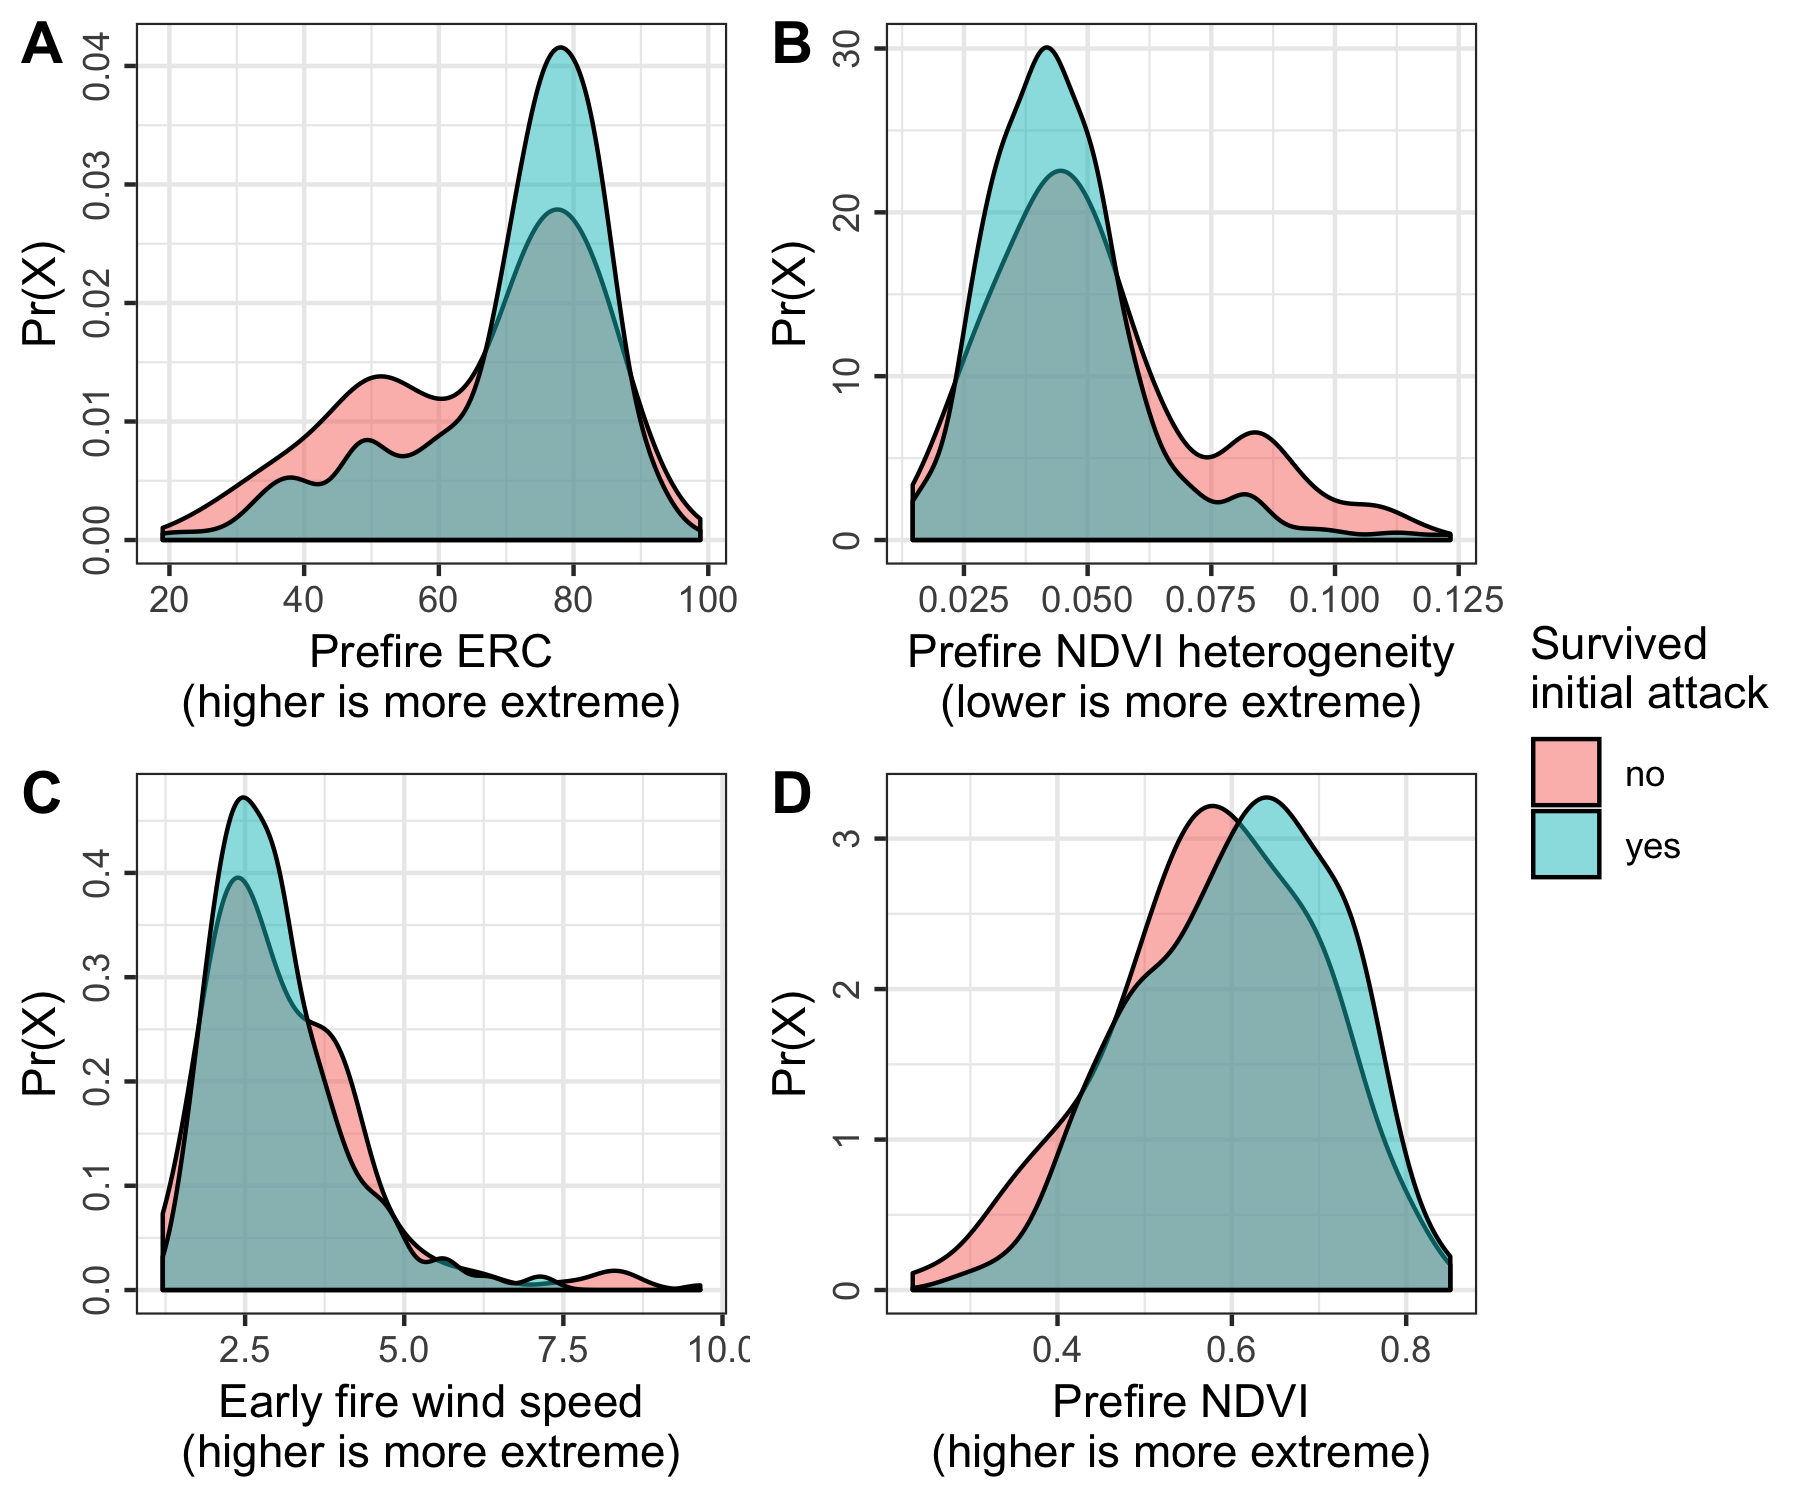
\includegraphics[width=6.00000in]{figure/chap03/selection-on-burning-conditions.png}
\caption{The selection effect on the vegetation and climate burning
conditions of suppressed wildfires. A) Early suppression efforts
selected for greater average energy release component (ERC), an estimate
of fireline intensity correlated to hot, dry conditions. B) Fires
surviving initial suppression efforts burn in more homogenous fuels, as
measured by the standard deviation of NDVI in a 90m x 90m window. C) We
detected no selection pressure on windspeed for the first 3 days of the
fire. D) We detected no selection pressure on prefire NDVI, which is
correlated with overstory canopy density and surface fuel loads.}
\end{figure}
\subsection{Implications of selection by suppression for fire
effects}\label{implications-of-selection-by-suppression-for-fire-effects}

We also found that fire effects of event size, proportion of high
severity, and stand replacing decay coefficient showed a similar trend
(i.e., slope) in suppression versus WFU fires as a function of burn
duration, except for those suppression fires with short burn durations.
However, the average fire effects (i.e., intercept) of suppression fires
tended to depart from effects of WFU fires and resulted in greater
proportion of high severity and a lower stand replacing decay
coefficient. The notable exception to these trends are suppression fires
with short burn durations, which experienced a strong selection pressure
on their burning conditions and whose fire effects were dramatically
different from fire effects of suppression fires that burned for longer.
Suppression fires that succumbed early to containment were much smaller,
had lower proportions of high severity, and had much higher stand
replacing decay coefficients than suppression fires that escaped initial
attack Figure 3.4). The fire effects of suppression fires that were
successfully contained were within the range of variation of WFU fires
for similar burn durations.
\begin{figure}
\centering
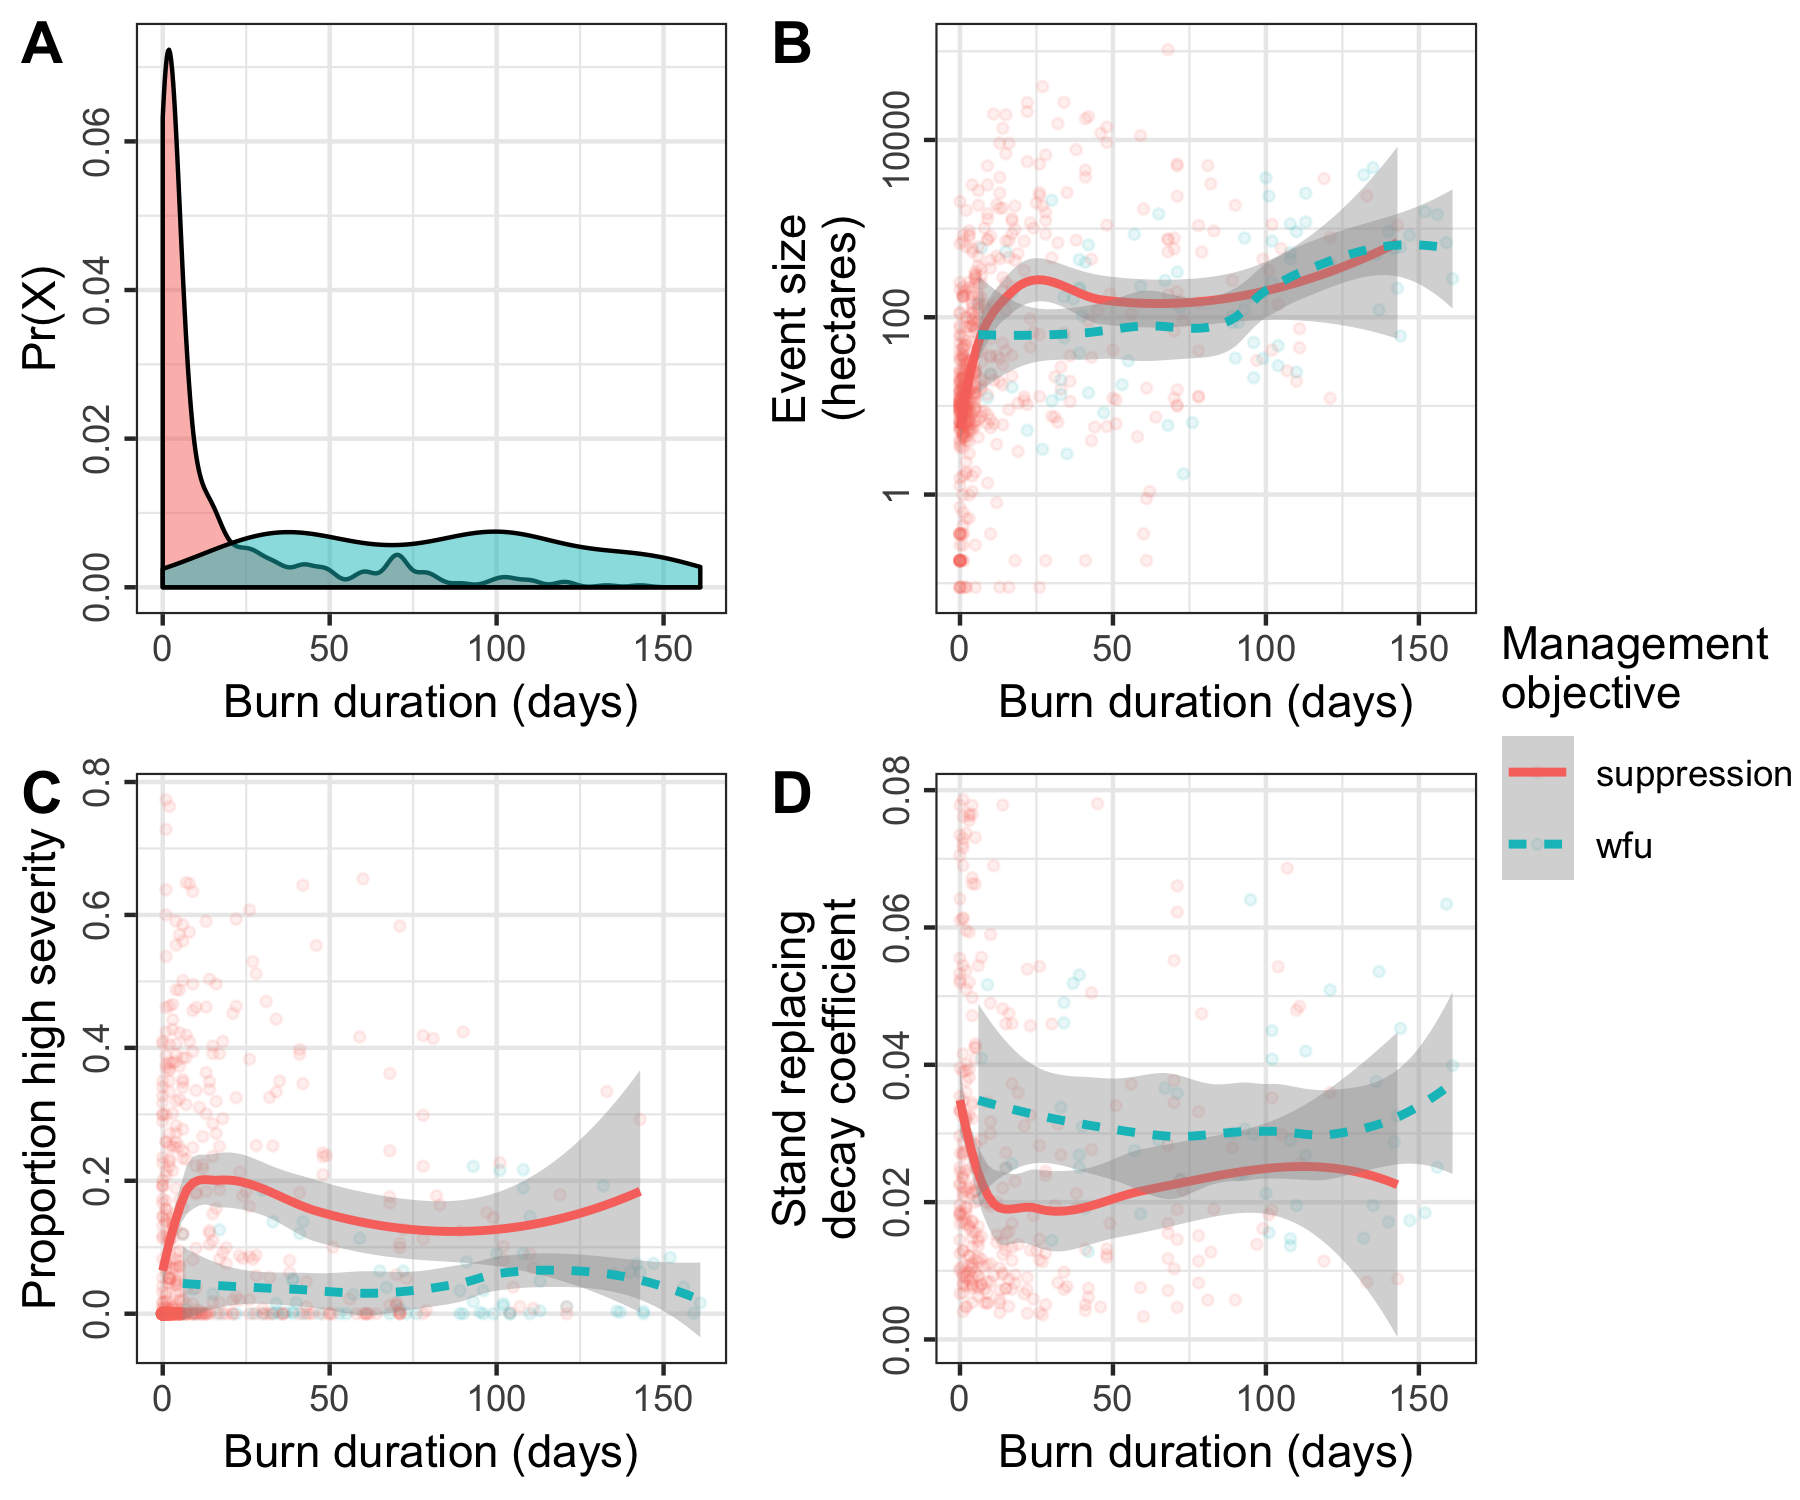
\includegraphics[width=6.00000in]{figure/chap03/burn-duration-4-panel.png}
\caption{A) Distribution of burn duration by management objective. Most
suppression fires are quickly extinguished. B) Effect of burn duration
on fire event size shows that there's a similar trajectory between
suppressed and wildfire use fires except early in the burning period
when suppression fires remain small. C) The high severity portion of the
fire tends to increase with shorter-duration suppression fires, but is
relatively constant across burn durations for wildfire use fires. D)
Conditional on a fire having a high-severity component, the stand
replacing decay coefficient sharply declines as burn duration increases
for suppression fires, indicating that the high-severity patches are
larger and simpler. Larger, simpler high-severity patches will have
reduced tree regeneration in their center because the distance to the
nearest tree seed source exceeds typical dispersal distances for yellow
pine/mixed-conifer species. The SDC tends to increase with the burn
duration for wildfire use fires.}
\end{figure}
\section{Discussion}\label{discussion-2}

Wildfire effects on forest vegetation are outcomes of a complex
social-ecological system dynamic (Calkin et al.
\protect\hyperlink{ref-calkin2015}{2015}). Direct causes of fire effects
to vegetation arise from fire behavior and intensity (Keeley
\protect\hyperlink{ref-keeley2009}{2009}), which are coupled to fuel,
weather, and topography (McKenzie and Hessl
\protect\hyperlink{ref-mckenzie2008}{2008}, Cansler and McKenzie
\protect\hyperlink{ref-cansler2014}{2014}, Harvey et al.
\protect\hyperlink{ref-harvey2016b}{2016}). Wildfire effects are
indirectly related to firefighting resource availability, legacies of
management policy that change fuel distributions, and incentive
structures that often prioritize mitigating short term loss of resources
over long-term benefits of wildfire (Houtman et al.
\protect\hyperlink{ref-houtman2013}{2013}, Calkin et al.
\protect\hyperlink{ref-calkin2014}{2014},
\protect\hyperlink{ref-calkin2015}{2015}). Fire suppression allows some
fires to ``survive'' initial containment efforts and contribute to fire
effects on the landscape, while other fires are ``killed'' by initial
containment and their potential fire effects are never realized. Because
milder fuel and climate conditions facilitate fire containment efforts,
initial attack suppression imposes selection for fires that burn under
more extreme conditions and shifts the concomitant distribution of fire
effects to also be more extreme. We measured this selection pressure and
found a sizable influence of initial suppression efforts that decreased
average fuel heterogeneity and increased average energy release
component for fires that contribute to fire effects on the landscape
(i.e., those that survive initial containment). Two primary implications
follow from our findings:
\begin{enumerate}
\def\labelenumi{\arabic{enumi})}
\item
  There is a lost contribution to overall fire effects in Sierra Nevada
  yellow pine/mixed-conifer forests associated with fires that are
  extinguished before they have a chance to burn under the milder
  conditions that facilitated their early containment (Figure 3.4).
\item
  The fire effects that are measured only on large fires reflect a
  selection bias imposed by suppression efforts (Figure 3.5).
\end{enumerate}
\begin{figure}
\centering
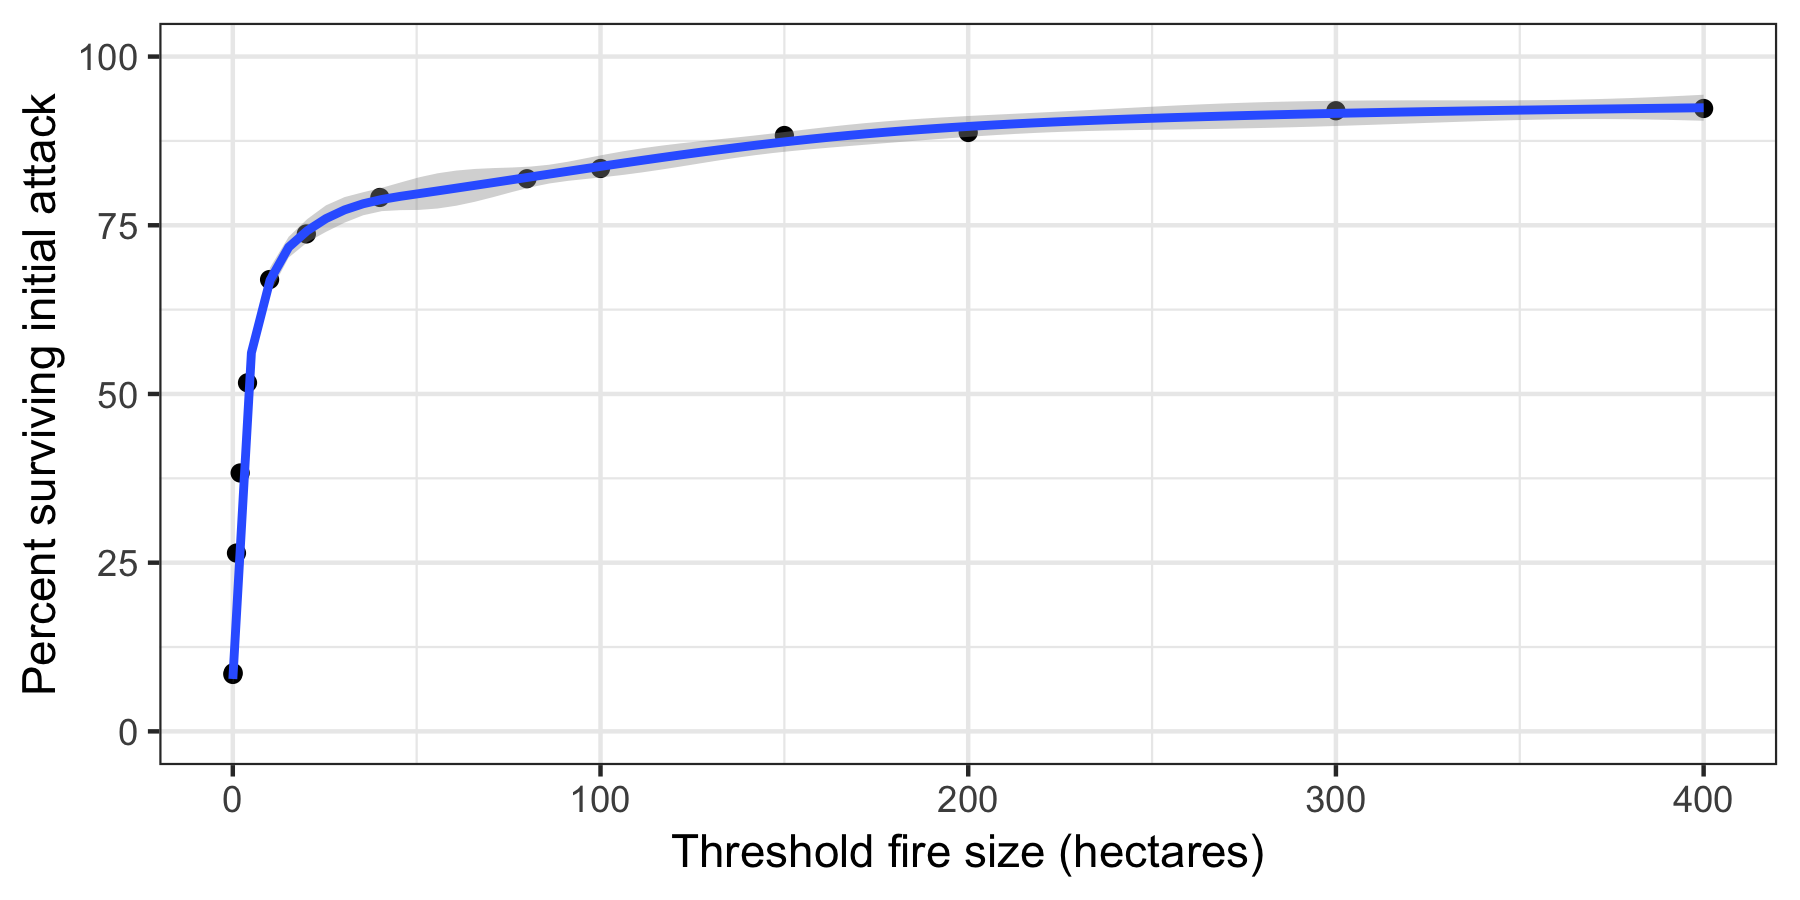
\includegraphics[width=6.00000in]{figure/chap03/prop-surviving-ia-by-size_short.png}
\caption{As the minimum fire event size of a dataset increases, a
greater proportion of those fire events survived initial attack
suppression efforts and burned on average under more extreme conditions.
Thus databases with larger minimum fire sizes exhibit a stronger bias
towards fires that burned in extreme conditions as a result of selection
by suppression.}
\end{figure}
\subsection{Context of suppression management on fire
effects}\label{context-of-suppression-management-on-fire-effects}

We compared fires managed for suppression to those managed for wildfire
use/resource benefit to assess how the selection pressure on burning
conditions may ultimately influence fire effects. We demonstrated a
clear multi-modality in the fire event size distribution of wildfires
managed with a suppression objective (Figure 3.1). The median fire size
of all fires in the dataset was much larger for WFU fires than for
suppression fires, but the median fire size of \emph{large} fires (e.g.,
fires greater than 80 or 400 hectares) was much larger for suppression
fires (Table 3.1). Miller and Safford
(\protect\hyperlink{ref-miller2017}{2017}) found a similar pattern in
comparing the average size of modern fires, most of which are managed
with a suppression objective, to pre-Euroamerican settlement fires--
modern, suppression fires are smaller on average compared to the natural
range of variation, but modern large fires are much larger compared to
the natural range of variation (Safford and Stevens
\protect\hyperlink{ref-safford2017}{2017}, Miller and Safford
\protect\hyperlink{ref-miller2017}{2017}).

Fire effects of escaped suppression fires were more departed from
effects of WFU fires for the same burn duration (Figure 3.4). However,
fire effects of suppression fires that succumbed to early suppression
efforts were generally beneficial when considering WFU fires as a
reference for beneficial effects. We cannot use our data to make a
rigorous counterfactual prediction of how suppression fires that didn't
survive initial attack may have ultimately influenced the overall
distribution of fire effects if they had been allowed to burn. However,
the detected selection by suppression effect for extreme burning
conditions suggests that, had these fires burned for longer, they may
have contributed to shifting the average fire effects of all suppression
fires closer to the observed fire effects for WFU fires (Figure 3.4).

\subsection{No detected effect of
windspeed}\label{no-detected-effect-of-windspeed}

Surprisingly, we found no selection pressure on wind speed by early
suppression efforts (Figure 3.2). Abatzoglou et al.
(\protect\hyperlink{ref-abatzoglou2018a}{2018}) found across the U.S.
that greater wind speeds during the first two days after human-caused
ignitions increased the likelihood that fires would grow large. Wind
speed may not reflect a limiting factor in early suppression efforts in
this region compared to fuel continuity and fuel moisture as measured by
energy release component. Alternatively, the gridMET-derived wind speed
in our study may be less representative of how wind affects fire
behavior in this particular system. That is, wind may play a strong
role, but the mountainous terrain may create more local wind conditions
than can be captured by the gridMET product, despite its high spatial
and temporal resolution (Abatzoglou
\protect\hyperlink{ref-abatzoglou2013}{2013}).

\subsection{Selection beyond initial
attack}\label{selection-beyond-initial-attack}

We demonstrated a strong directional effect of selection imposed by
initial suppression efforts on the initial burning conditions of
wildfires in the Sierra yellow pine/mixed-conifer system. Fire effects
arise from the confluence of fuel, weather, and topographical conditions
in space and time, and thus our event-level (i.e., per fire)
measurements of burning conditions may mask some of this selection
effect. We suspect this effect may be even stronger if weather
conditions were known at finer temporal scales and fuel conditions were
known at finer spatial scales. While we have shown a selection effect of
suppression during an initial attack response, the effect may not be
limited to soon after ignition (i.e., the scope of our investigation).
Whether a similar selection by suppression effect would materialize
beyond initial attack and \emph{throughout} the course of a fire's burn
duration depends on the extent to which success in suppression is
contingent upon fuel and weather conditions cooperating with
firefighting efforts. That is, preventing additional fire effects to the
landscape by extinguishing fires as soon as the weather or fuel
conditions become more conducive to suppression amounts to imposing a
similar selection effect that we detected during initial attack
suppression. Finer spatial and temporal resolution of burning conditions
(e.g., daily climate variables paired with daily fire spread/severity
maps) throughout the course of wildfires may help tune our understanding
of how management efforts can select for burning conditions. For
example, aggressive suppression management may impose the strongest
selection pressure on fuel and climate conditions from the day of or the
day prior to the fire. Alternatively, WFU management may impose the
strongest selection pressure on \emph{future} fuel and climate
conditions, which would reflect managers' efforts to guide the spread of
fire into forecasted, spatiotemporally favorable intersections of fuel
and climate.

\subsection{Positive feedbacks}\label{positive-feedbacks}

Selection for more extreme burning conditions favors future extreme
burning conditions in positive feedbacks of fuel and climate.
Homogeneous local forest structure makes this system more likely to burn
at high severity, with complete or nearly-complete mortality of
overstory vegetation (Koontz et al.
\protect\hyperlink{ref-koontz2019a}{2019}\protect\hyperlink{ref-koontz2019a}{b}).
While some high severity fire is expected (Safford and Stevens
\protect\hyperlink{ref-safford2017}{2017}), elevated average levels and
increased continuity of high-severity fire and make it more likely that
regenerating vegetation and future fuel structure will also be
homogeneous (North et al. \protect\hyperlink{ref-north2009a}{2009},
Coppoletta et al. \protect\hyperlink{ref-coppoletta2016}{2016}, Miller
and Safford \protect\hyperlink{ref-miller2017}{2017}, Stevens et al.
\protect\hyperlink{ref-stevens2017}{2017}). On longer time scales, the
selection by suppression for hotter/drier average burning conditions may
favor high-severity fire in the short run (Fried et al.
\protect\hyperlink{ref-fried2004}{2004}, Koontz et al.
\protect\hyperlink{ref-koontz2019a}{2019}\protect\hyperlink{ref-koontz2019a}{b}),
and may compromise forest recovery (Young et al.
\protect\hyperlink{ref-young2019}{2019}), carbon stock stability (Earles
et al. \protect\hyperlink{ref-earles2014}{2014}), and carbon
sequestration (Millar and Stephenson
\protect\hyperlink{ref-millar2015}{2015}) in the long run. A reduction
in carbon sequestration capacity contributes to climate forcing, which
is likely to perpetuate hot, dry conditions in California (Diffenbaugh
et al. \protect\hyperlink{ref-diffenbaugh2015}{2015}, Mann and Gleick
\protect\hyperlink{ref-mann2015}{2015}). Ongoing selection for extreme
burning conditions by fire suppression therefore creates positive
feedbacks of burning conditions that are unfavorable to yellow
pine/mixed-conifer forest persistence.

\subsection{A selection effect on WFU fires,
too}\label{a-selection-effect-on-wfu-fires-too}

A conceptually similar, but directionally opposite selection pressure
may bias the distribution of fire effects that arise from wildfire use
fires. The decision to let a candidate WFU ignition continue to burn as
a WFU fire when conditions are more mild selects for a distribution of
fire effects that arises from these more mild burning conditions. As
with the selection by suppression, the distribution of fire effects of
WFU fires will be dictated by the fires whose fire effects were allowed
to materialize (i.e., by deciding to let them burn in the WFU case
versus being unable to stop them from burning in the case of suppression
fires that escape initial attack). The fire effects from WFU fires are
largely seen as beneficial, but their average effect should be
considered as a better-than-average scenario for reintroducing fire to
previously fire-suppressed forests compared to the expectations of fire
effects if all candidate WFU ignitions were allowed to burn. Similarly,
the fire effects of suppression fires that escape initial attack are
largely seen as negative, but their average effect should be treated as
a worse-than-average scenario for reintroducing fire to the landscape
compared to fire effects that would arise from letting all ignitions run
their course.

The selection bias in both cases (suppression and WFU fires) reflects
the social element in the coupled social-ecological system of wildfire
and wildfire management. Management decisions, even as a fire burns, can
hold great sway over ultimate fire effects to the forest system in their
capacity to impose selection on the distribution of burning conditions.
However, the social element can also erect powerful barriers to more
widespread adoption of WFU fires such as consideration of smoke effects
on human health (Schweizer and Cisneros
\protect\hyperlink{ref-schweizer2014}{2014}) or political risks
associated with allowing fires to burn (Doane et al.
\protect\hyperlink{ref-doane2006}{2006}). The strong influence of
on-the-ground management decision-making points to the immense value of
reducing barriers to implementing more wildfire use fires through
increased training and reorganized incentive structures (Doane et al.
\protect\hyperlink{ref-doane2006}{2006}).

\section{Acknowledgements}\label{acknowledgements-2}

We thank Connie Millar for helpful comments that guided this work.

\chapter{\texorpdfstring{Appendix: Supplemental Information for `Chapter
1: Remote sensing
resistance'}{Appendix: Supplemental Information for Chapter 1: Remote sensing resistance}}\label{appendix-supplemental-information-for-chapter-1-remote-sensing-resistance}

\chaptermark{Supplementary information for Chapter 1}

\section{Supplemental methods}\label{supplemental-methods}

Normalized difference vegetation index (NDVI; Supplemental Equation 4.1)
correlates with vegetation density, canopy cover, and leaf area index
(Rouse et al. \protect\hyperlink{ref-rouse1973}{1973}). Normalized
difference moisture index (NDMI; Supplemental Equation 4.2) correlates
with similar vegetation characteristics as NDVI, but doesn't saturate at
high levels of foliar biomass (Gao
\protect\hyperlink{ref-gao1996}{1996}, Huesca et al.
(\protect\hyperlink{ref-huesca2016}{2016})). Normalized burn ratio (NBR;
Supplemental Equation 4.3) and normalized burn ratio version 2 (NBR2;
Supplemental Equation 4.4) respond strongly to fire effects on
vegetation (García and Caselles
\protect\hyperlink{ref-garcia1991}{1991}, Key and Benson
\protect\hyperlink{ref-key2006}{2006}, USGS
\protect\hyperlink{ref-usgs2017a}{2017}\protect\hyperlink{ref-usgs2017a}{a},
\protect\hyperlink{ref-usgs2017}{2017}\protect\hyperlink{ref-usgs2017}{b},
Hawbaker et al. \protect\hyperlink{ref-hawbaker2017}{2017}).

Supplemental Equation 4.1:
\(ndvi = \mathopen(nir - red\mathclose) / \mathopen(nir + red\mathclose)\)

Supplemental Equation 4.2:
\(ndmi = \mathopen(nir - swir1\mathclose) / \mathopen(nir + swir1\mathclose)\)

Supplemental Equation 4.3:
\(nbr = \mathopen(nir - swir2\mathclose) / \mathopen(nir + swir2\mathclose)\)

Supplemental Equation 4.4:
\(nbr2 = \mathopen(swir1 - swir2\mathclose) / \mathopen(swir1 + swir2\mathclose)\)

Where \(nir\) is the near infrared band (band 4 on Landsat 4, 5, and 7;
band 5 on Landsat 8) and \(red\) is the red band (band 3 on Landsat 4,
5, and 7; band 4 on Landsat 8), \(swir1\) is the first short wave
infrared band (band 5 on Landsat 4, 5, and 7; band 4 on Landsat 8),
\(swir2\) is the second short wave infrared band (band 7 on Landsat 4,
5, 7, and 8)

We calculated the delta severity indices (dNBR, dNBR2, dNDVI) by
subtracting the respective postfire indices from the prefire indices
(NBR, NBR2, and NDVI) without multiplying by a rescaling constant (e.g.,
we did not multiply the result by 1000 as in Miller and Thode
(\protect\hyperlink{ref-miller2007}{2007}); Supplemental Equation 4.5).
Following Reilly et al. (\protect\hyperlink{ref-reilly2017}{2017}), we
chose not to correct the delta indices using a phenological offset value
(typically calculated as the delta index in homogeneous forest patch
outside of the fire perimeter), as our approach implicitly accounts for
phenology by incorporating multiple cloud-free images across the same
time window both before the fire and one year later.

Supplemental Equation 4.5:
\(dI = I_{\text{prefire}} - I_{\text{postfire}}\)

We calculated the relative delta severity indices, RdNBR and RdNDVI, by
scaling the respective delta indices (dNBR and dNDVI) from Supplemental
Equation 4.6 by a square root transformation of the absolute value of
the prefire index.

Supplemental Equation 4.6:
\(RdI = \frac{dI}{\sqrt{abs(I_{\text{prefire}})}}\)

We calculated the relative burn ratio (RBR) following Parks et al.
(\protect\hyperlink{ref-parks2014a}{2014}) using Supplemental Equation
4.7.

Supplemental Equation 4.7:
\(RBR = \frac{dNBR}{NBR_{\text{prefire}} + 1.001}\)

We used the digital elevation model to calculate the potential annual
heat load (Supplemental Equation 4.8 at each pixel, which is an
integrated measure of latitude, slope, and a folding transformation of
aspect about the northeast-southwest line, such that northeast becomes 0
radians and southwest becomes \(\pi\) radians (McCune and Keon
\protect\hyperlink{ref-mccune2002}{2002}, with correction in McCune
\protect\hyperlink{ref-mccune2007}{2007}).

Supplemental Equation 4.8:

\(\begin{aligned} \label{eq-potential-annual-heat-load} aspect_{folded} &= abs( \pi - abs( aspect - \frac{5\pi}{4}) ) \\ log(pahl) &= \begin{aligned} &-1.467 + \\ &1.582 * cos(latitude) cos(slope) - \\ &1.5 * cos(aspect_{folded}) sin(slope) sin(latitude) - \\ &0.262 * sin(lat) sin(slope) + \\ &0.607 * sin(aspect_{folded}) sin(slope) \\ \end{aligned} \end{aligned}\)

Where \(pahl\) is the potential annual heat load, \(aspect_{folded}\) is
a transformation of aspect in radians, and both \(latitude\) and
\(slope\) are extracted from a digital elevation model with units of
radians.

\section{Supplemental figures and
tables}\label{supplemental-figures-and-tables}
\begin{longtable}[]{@{}ccccccccccc@{}}
\caption{Comparison of models used to validate and calibrate remotely
sensed wildfire severity with ground-based composite burn index (CBI)
severity sorted in descending order by the R\textsuperscript{2} value
from a 5-fold cross validation. A total of 56 models were tested
representing all possible combinations of 7 different measures of
wildfire severity (RBR, dNBR, dNBR2, RdNBR, RdNBR2, dNDVI, and RdNDVI),
4 different time windows in which Landsat imagery was acquired and
summarized with a median reducer on a pixel-by-pixel basis (16 days, 32
days, 48 days, and 64 days), and two different interpolation methods
(bilinear and bicubic). The three parameters (\(\beta_0\), \(\beta_1\),
and \(\beta_2\)) from the nonlinear model fit described in Eq. 1 are
reported. For each model, the value of the remotely sensed wildfire
severity measurement corresponding to the lower bounds of 3 commonly
used categories of severity are reported (`low' corresponds to a CBI
value of 0.1, `mod' corresponds to a CBI value of 1.25, and `high'
corresponds to a CBI value of 2.25)}\tabularnewline
\toprule
\begin{minipage}[b]{0.04\columnwidth}\centering\strut
Rank\strut
\end{minipage} & \begin{minipage}[b]{0.11\columnwidth}\centering\strut
Severity measure\strut
\end{minipage} & \begin{minipage}[b]{0.06\columnwidth}\centering\strut
Interp- olation\strut
\end{minipage} & \begin{minipage}[b]{0.08\columnwidth}\centering\strut
Time window\strut
\end{minipage} & \begin{minipage}[b]{0.08\columnwidth}\centering\strut
k-fold R\textsuperscript{2}\strut
\end{minipage} & \begin{minipage}[b]{0.07\columnwidth}\centering\strut
\(\beta_0\)\strut
\end{minipage} & \begin{minipage}[b]{0.07\columnwidth}\centering\strut
\(\beta_1\)\strut
\end{minipage} & \begin{minipage}[b]{0.07\columnwidth}\centering\strut
\(\beta_2\)\strut
\end{minipage} & \begin{minipage}[b]{0.05\columnwidth}\centering\strut
low\strut
\end{minipage} & \begin{minipage}[b]{0.05\columnwidth}\centering\strut
mod\strut
\end{minipage} & \begin{minipage}[b]{0.05\columnwidth}\centering\strut
high\strut
\end{minipage}\tabularnewline
\midrule
\endfirsthead
\toprule
\begin{minipage}[b]{0.04\columnwidth}\centering\strut
Rank\strut
\end{minipage} & \begin{minipage}[b]{0.11\columnwidth}\centering\strut
Severity measure\strut
\end{minipage} & \begin{minipage}[b]{0.06\columnwidth}\centering\strut
Interp- olation\strut
\end{minipage} & \begin{minipage}[b]{0.08\columnwidth}\centering\strut
Time window\strut
\end{minipage} & \begin{minipage}[b]{0.08\columnwidth}\centering\strut
k-fold R\textsuperscript{2}\strut
\end{minipage} & \begin{minipage}[b]{0.07\columnwidth}\centering\strut
\(\beta_0\)\strut
\end{minipage} & \begin{minipage}[b]{0.07\columnwidth}\centering\strut
\(\beta_1\)\strut
\end{minipage} & \begin{minipage}[b]{0.07\columnwidth}\centering\strut
\(\beta_2\)\strut
\end{minipage} & \begin{minipage}[b]{0.05\columnwidth}\centering\strut
low\strut
\end{minipage} & \begin{minipage}[b]{0.05\columnwidth}\centering\strut
mod\strut
\end{minipage} & \begin{minipage}[b]{0.05\columnwidth}\centering\strut
high\strut
\end{minipage}\tabularnewline
\midrule
\endhead
\begin{minipage}[t]{0.04\columnwidth}\centering\strut
1\strut
\end{minipage} & \begin{minipage}[t]{0.11\columnwidth}\centering\strut
RBR\strut
\end{minipage} & \begin{minipage}[t]{0.06\columnwidth}\centering\strut
bicubic\strut
\end{minipage} & \begin{minipage}[t]{0.08\columnwidth}\centering\strut
48\strut
\end{minipage} & \begin{minipage}[t]{0.08\columnwidth}\centering\strut
0.82\strut
\end{minipage} & \begin{minipage}[t]{0.07\columnwidth}\centering\strut
0.014\strut
\end{minipage} & \begin{minipage}[t]{0.07\columnwidth}\centering\strut
0.028\strut
\end{minipage} & \begin{minipage}[t]{0.07\columnwidth}\centering\strut
1.001\strut
\end{minipage} & \begin{minipage}[t]{0.05\columnwidth}\centering\strut
0.045\strut
\end{minipage} & \begin{minipage}[t]{0.05\columnwidth}\centering\strut
0.113\strut
\end{minipage} & \begin{minipage}[t]{0.05\columnwidth}\centering\strut
0.282\strut
\end{minipage}\tabularnewline
\begin{minipage}[t]{0.04\columnwidth}\centering\strut
2\strut
\end{minipage} & \begin{minipage}[t]{0.11\columnwidth}\centering\strut
RdNBR\strut
\end{minipage} & \begin{minipage}[t]{0.06\columnwidth}\centering\strut
bilinear\strut
\end{minipage} & \begin{minipage}[t]{0.08\columnwidth}\centering\strut
32\strut
\end{minipage} & \begin{minipage}[t]{0.08\columnwidth}\centering\strut
0.813\strut
\end{minipage} & \begin{minipage}[t]{0.07\columnwidth}\centering\strut
-0.483\strut
\end{minipage} & \begin{minipage}[t]{0.07\columnwidth}\centering\strut
3.061\strut
\end{minipage} & \begin{minipage}[t]{0.07\columnwidth}\centering\strut
0.857\strut
\end{minipage} & \begin{minipage}[t]{0.05\columnwidth}\centering\strut
2.852\strut
\end{minipage} & \begin{minipage}[t]{0.05\columnwidth}\centering\strut
8.45\strut
\end{minipage} & \begin{minipage}[t]{0.05\columnwidth}\centering\strut
20.56\strut
\end{minipage}\tabularnewline
\begin{minipage}[t]{0.04\columnwidth}\centering\strut
3\strut
\end{minipage} & \begin{minipage}[t]{0.11\columnwidth}\centering\strut
RdNDVI\strut
\end{minipage} & \begin{minipage}[t]{0.06\columnwidth}\centering\strut
bilinear\strut
\end{minipage} & \begin{minipage}[t]{0.08\columnwidth}\centering\strut
48\strut
\end{minipage} & \begin{minipage}[t]{0.08\columnwidth}\centering\strut
0.809\strut
\end{minipage} & \begin{minipage}[t]{0.07\columnwidth}\centering\strut
-2.144\strut
\end{minipage} & \begin{minipage}[t]{0.07\columnwidth}\centering\strut
3.273\strut
\end{minipage} & \begin{minipage}[t]{0.07\columnwidth}\centering\strut
0.609\strut
\end{minipage} & \begin{minipage}[t]{0.05\columnwidth}\centering\strut
1.335\strut
\end{minipage} & \begin{minipage}[t]{0.05\columnwidth}\centering\strut
4.867\strut
\end{minipage} & \begin{minipage}[t]{0.05\columnwidth}\centering\strut
10.75\strut
\end{minipage}\tabularnewline
\begin{minipage}[t]{0.04\columnwidth}\centering\strut
4\strut
\end{minipage} & \begin{minipage}[t]{0.11\columnwidth}\centering\strut
RBR\strut
\end{minipage} & \begin{minipage}[t]{0.06\columnwidth}\centering\strut
bilinear\strut
\end{minipage} & \begin{minipage}[t]{0.08\columnwidth}\centering\strut
32\strut
\end{minipage} & \begin{minipage}[t]{0.08\columnwidth}\centering\strut
0.807\strut
\end{minipage} & \begin{minipage}[t]{0.07\columnwidth}\centering\strut
0.014\strut
\end{minipage} & \begin{minipage}[t]{0.07\columnwidth}\centering\strut
0.029\strut
\end{minipage} & \begin{minipage}[t]{0.07\columnwidth}\centering\strut
0.985\strut
\end{minipage} & \begin{minipage}[t]{0.05\columnwidth}\centering\strut
0.046\strut
\end{minipage} & \begin{minipage}[t]{0.05\columnwidth}\centering\strut
0.113\strut
\end{minipage} & \begin{minipage}[t]{0.05\columnwidth}\centering\strut
0.28\strut
\end{minipage}\tabularnewline
\begin{minipage}[t]{0.04\columnwidth}\centering\strut
5\strut
\end{minipage} & \begin{minipage}[t]{0.11\columnwidth}\centering\strut
RdNDVI\strut
\end{minipage} & \begin{minipage}[t]{0.06\columnwidth}\centering\strut
bicubic\strut
\end{minipage} & \begin{minipage}[t]{0.08\columnwidth}\centering\strut
64\strut
\end{minipage} & \begin{minipage}[t]{0.08\columnwidth}\centering\strut
0.805\strut
\end{minipage} & \begin{minipage}[t]{0.07\columnwidth}\centering\strut
-2.524\strut
\end{minipage} & \begin{minipage}[t]{0.07\columnwidth}\centering\strut
3.57\strut
\end{minipage} & \begin{minipage}[t]{0.07\columnwidth}\centering\strut
0.59\strut
\end{minipage} & \begin{minipage}[t]{0.05\columnwidth}\centering\strut
1.263\strut
\end{minipage} & \begin{minipage}[t]{0.05\columnwidth}\centering\strut
4.936\strut
\end{minipage} & \begin{minipage}[t]{0.05\columnwidth}\centering\strut
10.93\strut
\end{minipage}\tabularnewline
\begin{minipage}[t]{0.04\columnwidth}\centering\strut
6\strut
\end{minipage} & \begin{minipage}[t]{0.11\columnwidth}\centering\strut
RBR\strut
\end{minipage} & \begin{minipage}[t]{0.06\columnwidth}\centering\strut
bicubic\strut
\end{minipage} & \begin{minipage}[t]{0.08\columnwidth}\centering\strut
64\strut
\end{minipage} & \begin{minipage}[t]{0.08\columnwidth}\centering\strut
0.805\strut
\end{minipage} & \begin{minipage}[t]{0.07\columnwidth}\centering\strut
0.016\strut
\end{minipage} & \begin{minipage}[t]{0.07\columnwidth}\centering\strut
0.027\strut
\end{minipage} & \begin{minipage}[t]{0.07\columnwidth}\centering\strut
1.01\strut
\end{minipage} & \begin{minipage}[t]{0.05\columnwidth}\centering\strut
0.046\strut
\end{minipage} & \begin{minipage}[t]{0.05\columnwidth}\centering\strut
0.113\strut
\end{minipage} & \begin{minipage}[t]{0.05\columnwidth}\centering\strut
0.283\strut
\end{minipage}\tabularnewline
\begin{minipage}[t]{0.04\columnwidth}\centering\strut
7\strut
\end{minipage} & \begin{minipage}[t]{0.11\columnwidth}\centering\strut
RdNDVI\strut
\end{minipage} & \begin{minipage}[t]{0.06\columnwidth}\centering\strut
bicubic\strut
\end{minipage} & \begin{minipage}[t]{0.08\columnwidth}\centering\strut
32\strut
\end{minipage} & \begin{minipage}[t]{0.08\columnwidth}\centering\strut
0.803\strut
\end{minipage} & \begin{minipage}[t]{0.07\columnwidth}\centering\strut
-2.737\strut
\end{minipage} & \begin{minipage}[t]{0.07\columnwidth}\centering\strut
3.308\strut
\end{minipage} & \begin{minipage}[t]{0.07\columnwidth}\centering\strut
0.619\strut
\end{minipage} & \begin{minipage}[t]{0.05\columnwidth}\centering\strut
0.782\strut
\end{minipage} & \begin{minipage}[t]{0.05\columnwidth}\centering\strut
4.436\strut
\end{minipage} & \begin{minipage}[t]{0.05\columnwidth}\centering\strut
10.59\strut
\end{minipage}\tabularnewline
\begin{minipage}[t]{0.04\columnwidth}\centering\strut
8\strut
\end{minipage} & \begin{minipage}[t]{0.11\columnwidth}\centering\strut
RBR\strut
\end{minipage} & \begin{minipage}[t]{0.06\columnwidth}\centering\strut
bilinear\strut
\end{minipage} & \begin{minipage}[t]{0.08\columnwidth}\centering\strut
64\strut
\end{minipage} & \begin{minipage}[t]{0.08\columnwidth}\centering\strut
0.802\strut
\end{minipage} & \begin{minipage}[t]{0.07\columnwidth}\centering\strut
0.017\strut
\end{minipage} & \begin{minipage}[t]{0.07\columnwidth}\centering\strut
0.027\strut
\end{minipage} & \begin{minipage}[t]{0.07\columnwidth}\centering\strut
1.003\strut
\end{minipage} & \begin{minipage}[t]{0.05\columnwidth}\centering\strut
0.047\strut
\end{minipage} & \begin{minipage}[t]{0.05\columnwidth}\centering\strut
0.113\strut
\end{minipage} & \begin{minipage}[t]{0.05\columnwidth}\centering\strut
0.279\strut
\end{minipage}\tabularnewline
\begin{minipage}[t]{0.04\columnwidth}\centering\strut
9\strut
\end{minipage} & \begin{minipage}[t]{0.11\columnwidth}\centering\strut
RdNDVI\strut
\end{minipage} & \begin{minipage}[t]{0.06\columnwidth}\centering\strut
bilinear\strut
\end{minipage} & \begin{minipage}[t]{0.08\columnwidth}\centering\strut
32\strut
\end{minipage} & \begin{minipage}[t]{0.08\columnwidth}\centering\strut
0.801\strut
\end{minipage} & \begin{minipage}[t]{0.07\columnwidth}\centering\strut
-2.531\strut
\end{minipage} & \begin{minipage}[t]{0.07\columnwidth}\centering\strut
3.176\strut
\end{minipage} & \begin{minipage}[t]{0.07\columnwidth}\centering\strut
0.624\strut
\end{minipage} & \begin{minipage}[t]{0.05\columnwidth}\centering\strut
0.849\strut
\end{minipage} & \begin{minipage}[t]{0.05\columnwidth}\centering\strut
4.393\strut
\end{minipage} & \begin{minipage}[t]{0.05\columnwidth}\centering\strut
10.39\strut
\end{minipage}\tabularnewline
\begin{minipage}[t]{0.04\columnwidth}\centering\strut
10\strut
\end{minipage} & \begin{minipage}[t]{0.11\columnwidth}\centering\strut
RdNDVI\strut
\end{minipage} & \begin{minipage}[t]{0.06\columnwidth}\centering\strut
bicubic\strut
\end{minipage} & \begin{minipage}[t]{0.08\columnwidth}\centering\strut
48\strut
\end{minipage} & \begin{minipage}[t]{0.08\columnwidth}\centering\strut
0.797\strut
\end{minipage} & \begin{minipage}[t]{0.07\columnwidth}\centering\strut
-2.623\strut
\end{minipage} & \begin{minipage}[t]{0.07\columnwidth}\centering\strut
3.624\strut
\end{minipage} & \begin{minipage}[t]{0.07\columnwidth}\centering\strut
0.587\strut
\end{minipage} & \begin{minipage}[t]{0.05\columnwidth}\centering\strut
1.22\strut
\end{minipage} & \begin{minipage}[t]{0.05\columnwidth}\centering\strut
4.922\strut
\end{minipage} & \begin{minipage}[t]{0.05\columnwidth}\centering\strut
10.94\strut
\end{minipage}\tabularnewline
\begin{minipage}[t]{0.04\columnwidth}\centering\strut
11\strut
\end{minipage} & \begin{minipage}[t]{0.11\columnwidth}\centering\strut
RdNDVI\strut
\end{minipage} & \begin{minipage}[t]{0.06\columnwidth}\centering\strut
bilinear\strut
\end{minipage} & \begin{minipage}[t]{0.08\columnwidth}\centering\strut
64\strut
\end{minipage} & \begin{minipage}[t]{0.08\columnwidth}\centering\strut
0.796\strut
\end{minipage} & \begin{minipage}[t]{0.07\columnwidth}\centering\strut
-2.14\strut
\end{minipage} & \begin{minipage}[t]{0.07\columnwidth}\centering\strut
3.287\strut
\end{minipage} & \begin{minipage}[t]{0.07\columnwidth}\centering\strut
0.607\strut
\end{minipage} & \begin{minipage}[t]{0.05\columnwidth}\centering\strut
1.353\strut
\end{minipage} & \begin{minipage}[t]{0.05\columnwidth}\centering\strut
4.876\strut
\end{minipage} & \begin{minipage}[t]{0.05\columnwidth}\centering\strut
10.73\strut
\end{minipage}\tabularnewline
\begin{minipage}[t]{0.04\columnwidth}\centering\strut
12\strut
\end{minipage} & \begin{minipage}[t]{0.11\columnwidth}\centering\strut
RdNBR\strut
\end{minipage} & \begin{minipage}[t]{0.06\columnwidth}\centering\strut
bilinear\strut
\end{minipage} & \begin{minipage}[t]{0.08\columnwidth}\centering\strut
64\strut
\end{minipage} & \begin{minipage}[t]{0.08\columnwidth}\centering\strut
0.792\strut
\end{minipage} & \begin{minipage}[t]{0.07\columnwidth}\centering\strut
-0.42\strut
\end{minipage} & \begin{minipage}[t]{0.07\columnwidth}\centering\strut
3.031\strut
\end{minipage} & \begin{minipage}[t]{0.07\columnwidth}\centering\strut
0.862\strut
\end{minipage} & \begin{minipage}[t]{0.05\columnwidth}\centering\strut
2.884\strut
\end{minipage} & \begin{minipage}[t]{0.05\columnwidth}\centering\strut
8.483\strut
\end{minipage} & \begin{minipage}[t]{0.05\columnwidth}\centering\strut
20.66\strut
\end{minipage}\tabularnewline
\begin{minipage}[t]{0.04\columnwidth}\centering\strut
13\strut
\end{minipage} & \begin{minipage}[t]{0.11\columnwidth}\centering\strut
RBR\strut
\end{minipage} & \begin{minipage}[t]{0.06\columnwidth}\centering\strut
bilinear\strut
\end{minipage} & \begin{minipage}[t]{0.08\columnwidth}\centering\strut
48\strut
\end{minipage} & \begin{minipage}[t]{0.08\columnwidth}\centering\strut
0.791\strut
\end{minipage} & \begin{minipage}[t]{0.07\columnwidth}\centering\strut
0.017\strut
\end{minipage} & \begin{minipage}[t]{0.07\columnwidth}\centering\strut
0.027\strut
\end{minipage} & \begin{minipage}[t]{0.07\columnwidth}\centering\strut
1.006\strut
\end{minipage} & \begin{minipage}[t]{0.05\columnwidth}\centering\strut
0.047\strut
\end{minipage} & \begin{minipage}[t]{0.05\columnwidth}\centering\strut
0.112\strut
\end{minipage} & \begin{minipage}[t]{0.05\columnwidth}\centering\strut
0.277\strut
\end{minipage}\tabularnewline
\begin{minipage}[t]{0.04\columnwidth}\centering\strut
14\strut
\end{minipage} & \begin{minipage}[t]{0.11\columnwidth}\centering\strut
RBR\strut
\end{minipage} & \begin{minipage}[t]{0.06\columnwidth}\centering\strut
bicubic\strut
\end{minipage} & \begin{minipage}[t]{0.08\columnwidth}\centering\strut
32\strut
\end{minipage} & \begin{minipage}[t]{0.08\columnwidth}\centering\strut
0.79\strut
\end{minipage} & \begin{minipage}[t]{0.07\columnwidth}\centering\strut
0.013\strut
\end{minipage} & \begin{minipage}[t]{0.07\columnwidth}\centering\strut
0.029\strut
\end{minipage} & \begin{minipage}[t]{0.07\columnwidth}\centering\strut
0.994\strut
\end{minipage} & \begin{minipage}[t]{0.05\columnwidth}\centering\strut
0.045\strut
\end{minipage} & \begin{minipage}[t]{0.05\columnwidth}\centering\strut
0.114\strut
\end{minipage} & \begin{minipage}[t]{0.05\columnwidth}\centering\strut
0.284\strut
\end{minipage}\tabularnewline
\begin{minipage}[t]{0.04\columnwidth}\centering\strut
15\strut
\end{minipage} & \begin{minipage}[t]{0.11\columnwidth}\centering\strut
RdNBR\strut
\end{minipage} & \begin{minipage}[t]{0.06\columnwidth}\centering\strut
bicubic\strut
\end{minipage} & \begin{minipage}[t]{0.08\columnwidth}\centering\strut
48\strut
\end{minipage} & \begin{minipage}[t]{0.08\columnwidth}\centering\strut
0.785\strut
\end{minipage} & \begin{minipage}[t]{0.07\columnwidth}\centering\strut
-0.858\strut
\end{minipage} & \begin{minipage}[t]{0.07\columnwidth}\centering\strut
3.219\strut
\end{minipage} & \begin{minipage}[t]{0.07\columnwidth}\centering\strut
0.852\strut
\end{minipage} & \begin{minipage}[t]{0.05\columnwidth}\centering\strut
2.647\strut
\end{minipage} & \begin{minipage}[t]{0.05\columnwidth}\centering\strut
8.476\strut
\end{minipage} & \begin{minipage}[t]{0.05\columnwidth}\centering\strut
21.02\strut
\end{minipage}\tabularnewline
\begin{minipage}[t]{0.04\columnwidth}\centering\strut
16\strut
\end{minipage} & \begin{minipage}[t]{0.11\columnwidth}\centering\strut
RBR\strut
\end{minipage} & \begin{minipage}[t]{0.06\columnwidth}\centering\strut
bilinear\strut
\end{minipage} & \begin{minipage}[t]{0.08\columnwidth}\centering\strut
16\strut
\end{minipage} & \begin{minipage}[t]{0.08\columnwidth}\centering\strut
0.781\strut
\end{minipage} & \begin{minipage}[t]{0.07\columnwidth}\centering\strut
0.021\strut
\end{minipage} & \begin{minipage}[t]{0.07\columnwidth}\centering\strut
0.026\strut
\end{minipage} & \begin{minipage}[t]{0.07\columnwidth}\centering\strut
1.016\strut
\end{minipage} & \begin{minipage}[t]{0.05\columnwidth}\centering\strut
0.05\strut
\end{minipage} & \begin{minipage}[t]{0.05\columnwidth}\centering\strut
0.114\strut
\end{minipage} & \begin{minipage}[t]{0.05\columnwidth}\centering\strut
0.278\strut
\end{minipage}\tabularnewline
\begin{minipage}[t]{0.04\columnwidth}\centering\strut
17\strut
\end{minipage} & \begin{minipage}[t]{0.11\columnwidth}\centering\strut
RdNBR\strut
\end{minipage} & \begin{minipage}[t]{0.06\columnwidth}\centering\strut
bicubic\strut
\end{minipage} & \begin{minipage}[t]{0.08\columnwidth}\centering\strut
32\strut
\end{minipage} & \begin{minipage}[t]{0.08\columnwidth}\centering\strut
0.776\strut
\end{minipage} & \begin{minipage}[t]{0.07\columnwidth}\centering\strut
-0.954\strut
\end{minipage} & \begin{minipage}[t]{0.07\columnwidth}\centering\strut
3.34\strut
\end{minipage} & \begin{minipage}[t]{0.07\columnwidth}\centering\strut
0.841\strut
\end{minipage} & \begin{minipage}[t]{0.05\columnwidth}\centering\strut
2.679\strut
\end{minipage} & \begin{minipage}[t]{0.05\columnwidth}\centering\strut
8.602\strut
\end{minipage} & \begin{minipage}[t]{0.05\columnwidth}\centering\strut
21.2\strut
\end{minipage}\tabularnewline
\begin{minipage}[t]{0.04\columnwidth}\centering\strut
18\strut
\end{minipage} & \begin{minipage}[t]{0.11\columnwidth}\centering\strut
dNDVI\strut
\end{minipage} & \begin{minipage}[t]{0.06\columnwidth}\centering\strut
bicubic\strut
\end{minipage} & \begin{minipage}[t]{0.08\columnwidth}\centering\strut
32\strut
\end{minipage} & \begin{minipage}[t]{0.08\columnwidth}\centering\strut
0.776\strut
\end{minipage} & \begin{minipage}[t]{0.07\columnwidth}\centering\strut
-0.058\strut
\end{minipage} & \begin{minipage}[t]{0.07\columnwidth}\centering\strut
0.073\strut
\end{minipage} & \begin{minipage}[t]{0.07\columnwidth}\centering\strut
0.65\strut
\end{minipage} & \begin{minipage}[t]{0.05\columnwidth}\centering\strut
0.02\strut
\end{minipage} & \begin{minipage}[t]{0.05\columnwidth}\centering\strut
0.106\strut
\end{minipage} & \begin{minipage}[t]{0.05\columnwidth}\centering\strut
0.257\strut
\end{minipage}\tabularnewline
\begin{minipage}[t]{0.04\columnwidth}\centering\strut
19\strut
\end{minipage} & \begin{minipage}[t]{0.11\columnwidth}\centering\strut
dNBR\strut
\end{minipage} & \begin{minipage}[t]{0.06\columnwidth}\centering\strut
bicubic\strut
\end{minipage} & \begin{minipage}[t]{0.08\columnwidth}\centering\strut
48\strut
\end{minipage} & \begin{minipage}[t]{0.08\columnwidth}\centering\strut
0.775\strut
\end{minipage} & \begin{minipage}[t]{0.07\columnwidth}\centering\strut
0.03\strut
\end{minipage} & \begin{minipage}[t]{0.07\columnwidth}\centering\strut
0.035\strut
\end{minipage} & \begin{minipage}[t]{0.07\columnwidth}\centering\strut
1.069\strut
\end{minipage} & \begin{minipage}[t]{0.05\columnwidth}\centering\strut
0.068\strut
\end{minipage} & \begin{minipage}[t]{0.05\columnwidth}\centering\strut
0.161\strut
\end{minipage} & \begin{minipage}[t]{0.05\columnwidth}\centering\strut
0.413\strut
\end{minipage}\tabularnewline
\begin{minipage}[t]{0.04\columnwidth}\centering\strut
20\strut
\end{minipage} & \begin{minipage}[t]{0.11\columnwidth}\centering\strut
RdNBR\strut
\end{minipage} & \begin{minipage}[t]{0.06\columnwidth}\centering\strut
bilinear\strut
\end{minipage} & \begin{minipage}[t]{0.08\columnwidth}\centering\strut
16\strut
\end{minipage} & \begin{minipage}[t]{0.08\columnwidth}\centering\strut
0.774\strut
\end{minipage} & \begin{minipage}[t]{0.07\columnwidth}\centering\strut
0.279\strut
\end{minipage} & \begin{minipage}[t]{0.07\columnwidth}\centering\strut
2.518\strut
\end{minipage} & \begin{minipage}[t]{0.07\columnwidth}\centering\strut
0.909\strut
\end{minipage} & \begin{minipage}[t]{0.05\columnwidth}\centering\strut
3.037\strut
\end{minipage} & \begin{minipage}[t]{0.05\columnwidth}\centering\strut
8.119\strut
\end{minipage} & \begin{minipage}[t]{0.05\columnwidth}\centering\strut
19.73\strut
\end{minipage}\tabularnewline
\begin{minipage}[t]{0.04\columnwidth}\centering\strut
21\strut
\end{minipage} & \begin{minipage}[t]{0.11\columnwidth}\centering\strut
dNDVI\strut
\end{minipage} & \begin{minipage}[t]{0.06\columnwidth}\centering\strut
bilinear\strut
\end{minipage} & \begin{minipage}[t]{0.08\columnwidth}\centering\strut
32\strut
\end{minipage} & \begin{minipage}[t]{0.08\columnwidth}\centering\strut
0.772\strut
\end{minipage} & \begin{minipage}[t]{0.07\columnwidth}\centering\strut
-0.053\strut
\end{minipage} & \begin{minipage}[t]{0.07\columnwidth}\centering\strut
0.07\strut
\end{minipage} & \begin{minipage}[t]{0.07\columnwidth}\centering\strut
0.656\strut
\end{minipage} & \begin{minipage}[t]{0.05\columnwidth}\centering\strut
0.022\strut
\end{minipage} & \begin{minipage}[t]{0.05\columnwidth}\centering\strut
0.105\strut
\end{minipage} & \begin{minipage}[t]{0.05\columnwidth}\centering\strut
0.252\strut
\end{minipage}\tabularnewline
\begin{minipage}[t]{0.04\columnwidth}\centering\strut
22\strut
\end{minipage} & \begin{minipage}[t]{0.11\columnwidth}\centering\strut
dNDVI\strut
\end{minipage} & \begin{minipage}[t]{0.06\columnwidth}\centering\strut
bicubic\strut
\end{minipage} & \begin{minipage}[t]{0.08\columnwidth}\centering\strut
48\strut
\end{minipage} & \begin{minipage}[t]{0.08\columnwidth}\centering\strut
0.772\strut
\end{minipage} & \begin{minipage}[t]{0.07\columnwidth}\centering\strut
-0.055\strut
\end{minipage} & \begin{minipage}[t]{0.07\columnwidth}\centering\strut
0.081\strut
\end{minipage} & \begin{minipage}[t]{0.07\columnwidth}\centering\strut
0.613\strut
\end{minipage} & \begin{minipage}[t]{0.05\columnwidth}\centering\strut
0.031\strut
\end{minipage} & \begin{minipage}[t]{0.05\columnwidth}\centering\strut
0.119\strut
\end{minipage} & \begin{minipage}[t]{0.05\columnwidth}\centering\strut
0.267\strut
\end{minipage}\tabularnewline
\begin{minipage}[t]{0.04\columnwidth}\centering\strut
23\strut
\end{minipage} & \begin{minipage}[t]{0.11\columnwidth}\centering\strut
dNBR\strut
\end{minipage} & \begin{minipage}[t]{0.06\columnwidth}\centering\strut
bilinear\strut
\end{minipage} & \begin{minipage}[t]{0.08\columnwidth}\centering\strut
32\strut
\end{minipage} & \begin{minipage}[t]{0.08\columnwidth}\centering\strut
0.77\strut
\end{minipage} & \begin{minipage}[t]{0.07\columnwidth}\centering\strut
0.029\strut
\end{minipage} & \begin{minipage}[t]{0.07\columnwidth}\centering\strut
0.036\strut
\end{minipage} & \begin{minipage}[t]{0.07\columnwidth}\centering\strut
1.048\strut
\end{minipage} & \begin{minipage}[t]{0.05\columnwidth}\centering\strut
0.069\strut
\end{minipage} & \begin{minipage}[t]{0.05\columnwidth}\centering\strut
0.163\strut
\end{minipage} & \begin{minipage}[t]{0.05\columnwidth}\centering\strut
0.41\strut
\end{minipage}\tabularnewline
\begin{minipage}[t]{0.04\columnwidth}\centering\strut
24\strut
\end{minipage} & \begin{minipage}[t]{0.11\columnwidth}\centering\strut
RdNBR2\strut
\end{minipage} & \begin{minipage}[t]{0.06\columnwidth}\centering\strut
bicubic\strut
\end{minipage} & \begin{minipage}[t]{0.08\columnwidth}\centering\strut
64\strut
\end{minipage} & \begin{minipage}[t]{0.08\columnwidth}\centering\strut
0.766\strut
\end{minipage} & \begin{minipage}[t]{0.07\columnwidth}\centering\strut
2.102\strut
\end{minipage} & \begin{minipage}[t]{0.07\columnwidth}\centering\strut
0.416\strut
\end{minipage} & \begin{minipage}[t]{0.07\columnwidth}\centering\strut
1.24\strut
\end{minipage} & \begin{minipage}[t]{0.05\columnwidth}\centering\strut
2.572\strut
\end{minipage} & \begin{minipage}[t]{0.05\columnwidth}\centering\strut
4.059\strut
\end{minipage} & \begin{minipage}[t]{0.05\columnwidth}\centering\strut
8.861\strut
\end{minipage}\tabularnewline
\begin{minipage}[t]{0.04\columnwidth}\centering\strut
25\strut
\end{minipage} & \begin{minipage}[t]{0.11\columnwidth}\centering\strut
dNBR\strut
\end{minipage} & \begin{minipage}[t]{0.06\columnwidth}\centering\strut
bicubic\strut
\end{minipage} & \begin{minipage}[t]{0.08\columnwidth}\centering\strut
32\strut
\end{minipage} & \begin{minipage}[t]{0.08\columnwidth}\centering\strut
0.764\strut
\end{minipage} & \begin{minipage}[t]{0.07\columnwidth}\centering\strut
0.028\strut
\end{minipage} & \begin{minipage}[t]{0.07\columnwidth}\centering\strut
0.036\strut
\end{minipage} & \begin{minipage}[t]{0.07\columnwidth}\centering\strut
1.057\strut
\end{minipage} & \begin{minipage}[t]{0.05\columnwidth}\centering\strut
0.068\strut
\end{minipage} & \begin{minipage}[t]{0.05\columnwidth}\centering\strut
0.163\strut
\end{minipage} & \begin{minipage}[t]{0.05\columnwidth}\centering\strut
0.417\strut
\end{minipage}\tabularnewline
\begin{minipage}[t]{0.04\columnwidth}\centering\strut
26\strut
\end{minipage} & \begin{minipage}[t]{0.11\columnwidth}\centering\strut
dNDVI\strut
\end{minipage} & \begin{minipage}[t]{0.06\columnwidth}\centering\strut
bilinear\strut
\end{minipage} & \begin{minipage}[t]{0.08\columnwidth}\centering\strut
48\strut
\end{minipage} & \begin{minipage}[t]{0.08\columnwidth}\centering\strut
0.762\strut
\end{minipage} & \begin{minipage}[t]{0.07\columnwidth}\centering\strut
-0.044\strut
\end{minipage} & \begin{minipage}[t]{0.07\columnwidth}\centering\strut
0.073\strut
\end{minipage} & \begin{minipage}[t]{0.07\columnwidth}\centering\strut
0.637\strut
\end{minipage} & \begin{minipage}[t]{0.05\columnwidth}\centering\strut
0.034\strut
\end{minipage} & \begin{minipage}[t]{0.05\columnwidth}\centering\strut
0.118\strut
\end{minipage} & \begin{minipage}[t]{0.05\columnwidth}\centering\strut
0.262\strut
\end{minipage}\tabularnewline
\begin{minipage}[t]{0.04\columnwidth}\centering\strut
27\strut
\end{minipage} & \begin{minipage}[t]{0.11\columnwidth}\centering\strut
RBR\strut
\end{minipage} & \begin{minipage}[t]{0.06\columnwidth}\centering\strut
bicubic\strut
\end{minipage} & \begin{minipage}[t]{0.08\columnwidth}\centering\strut
16\strut
\end{minipage} & \begin{minipage}[t]{0.08\columnwidth}\centering\strut
0.761\strut
\end{minipage} & \begin{minipage}[t]{0.07\columnwidth}\centering\strut
0.021\strut
\end{minipage} & \begin{minipage}[t]{0.07\columnwidth}\centering\strut
0.026\strut
\end{minipage} & \begin{minipage}[t]{0.07\columnwidth}\centering\strut
1.028\strut
\end{minipage} & \begin{minipage}[t]{0.05\columnwidth}\centering\strut
0.049\strut
\end{minipage} & \begin{minipage}[t]{0.05\columnwidth}\centering\strut
0.114\strut
\end{minipage} & \begin{minipage}[t]{0.05\columnwidth}\centering\strut
0.281\strut
\end{minipage}\tabularnewline
\begin{minipage}[t]{0.04\columnwidth}\centering\strut
28\strut
\end{minipage} & \begin{minipage}[t]{0.11\columnwidth}\centering\strut
dNBR\strut
\end{minipage} & \begin{minipage}[t]{0.06\columnwidth}\centering\strut
bilinear\strut
\end{minipage} & \begin{minipage}[t]{0.08\columnwidth}\centering\strut
16\strut
\end{minipage} & \begin{minipage}[t]{0.08\columnwidth}\centering\strut
0.76\strut
\end{minipage} & \begin{minipage}[t]{0.07\columnwidth}\centering\strut
0.033\strut
\end{minipage} & \begin{minipage}[t]{0.07\columnwidth}\centering\strut
0.036\strut
\end{minipage} & \begin{minipage}[t]{0.07\columnwidth}\centering\strut
1.048\strut
\end{minipage} & \begin{minipage}[t]{0.05\columnwidth}\centering\strut
0.073\strut
\end{minipage} & \begin{minipage}[t]{0.05\columnwidth}\centering\strut
0.167\strut
\end{minipage} & \begin{minipage}[t]{0.05\columnwidth}\centering\strut
0.417\strut
\end{minipage}\tabularnewline
\begin{minipage}[t]{0.04\columnwidth}\centering\strut
29\strut
\end{minipage} & \begin{minipage}[t]{0.11\columnwidth}\centering\strut
RdNBR2\strut
\end{minipage} & \begin{minipage}[t]{0.06\columnwidth}\centering\strut
bilinear\strut
\end{minipage} & \begin{minipage}[t]{0.08\columnwidth}\centering\strut
32\strut
\end{minipage} & \begin{minipage}[t]{0.08\columnwidth}\centering\strut
0.759\strut
\end{minipage} & \begin{minipage}[t]{0.07\columnwidth}\centering\strut
1.435\strut
\end{minipage} & \begin{minipage}[t]{0.07\columnwidth}\centering\strut
0.625\strut
\end{minipage} & \begin{minipage}[t]{0.07\columnwidth}\centering\strut
1.1\strut
\end{minipage} & \begin{minipage}[t]{0.05\columnwidth}\centering\strut
2.132\strut
\end{minipage} & \begin{minipage}[t]{0.05\columnwidth}\centering\strut
3.906\strut
\end{minipage} & \begin{minipage}[t]{0.05\columnwidth}\centering\strut
8.861\strut
\end{minipage}\tabularnewline
\begin{minipage}[t]{0.04\columnwidth}\centering\strut
30\strut
\end{minipage} & \begin{minipage}[t]{0.11\columnwidth}\centering\strut
RdNBR\strut
\end{minipage} & \begin{minipage}[t]{0.06\columnwidth}\centering\strut
bicubic\strut
\end{minipage} & \begin{minipage}[t]{0.08\columnwidth}\centering\strut
16\strut
\end{minipage} & \begin{minipage}[t]{0.08\columnwidth}\centering\strut
0.758\strut
\end{minipage} & \begin{minipage}[t]{0.07\columnwidth}\centering\strut
0.37\strut
\end{minipage} & \begin{minipage}[t]{0.07\columnwidth}\centering\strut
2.446\strut
\end{minipage} & \begin{minipage}[t]{0.07\columnwidth}\centering\strut
0.926\strut
\end{minipage} & \begin{minipage}[t]{0.05\columnwidth}\centering\strut
3.053\strut
\end{minipage} & \begin{minipage}[t]{0.05\columnwidth}\centering\strut
8.149\strut
\end{minipage} & \begin{minipage}[t]{0.05\columnwidth}\centering\strut
20\strut
\end{minipage}\tabularnewline
\begin{minipage}[t]{0.04\columnwidth}\centering\strut
31\strut
\end{minipage} & \begin{minipage}[t]{0.11\columnwidth}\centering\strut
RdNBR2\strut
\end{minipage} & \begin{minipage}[t]{0.06\columnwidth}\centering\strut
bicubic\strut
\end{minipage} & \begin{minipage}[t]{0.08\columnwidth}\centering\strut
32\strut
\end{minipage} & \begin{minipage}[t]{0.08\columnwidth}\centering\strut
0.754\strut
\end{minipage} & \begin{minipage}[t]{0.07\columnwidth}\centering\strut
1.426\strut
\end{minipage} & \begin{minipage}[t]{0.07\columnwidth}\centering\strut
0.601\strut
\end{minipage} & \begin{minipage}[t]{0.07\columnwidth}\centering\strut
1.125\strut
\end{minipage} & \begin{minipage}[t]{0.05\columnwidth}\centering\strut
2.098\strut
\end{minipage} & \begin{minipage}[t]{0.05\columnwidth}\centering\strut
3.876\strut
\end{minipage} & \begin{minipage}[t]{0.05\columnwidth}\centering\strut
8.975\strut
\end{minipage}\tabularnewline
\begin{minipage}[t]{0.04\columnwidth}\centering\strut
32\strut
\end{minipage} & \begin{minipage}[t]{0.11\columnwidth}\centering\strut
dNBR\strut
\end{minipage} & \begin{minipage}[t]{0.06\columnwidth}\centering\strut
bicubic\strut
\end{minipage} & \begin{minipage}[t]{0.08\columnwidth}\centering\strut
64\strut
\end{minipage} & \begin{minipage}[t]{0.08\columnwidth}\centering\strut
0.753\strut
\end{minipage} & \begin{minipage}[t]{0.07\columnwidth}\centering\strut
0.033\strut
\end{minipage} & \begin{minipage}[t]{0.07\columnwidth}\centering\strut
0.033\strut
\end{minipage} & \begin{minipage}[t]{0.07\columnwidth}\centering\strut
1.086\strut
\end{minipage} & \begin{minipage}[t]{0.05\columnwidth}\centering\strut
0.07\strut
\end{minipage} & \begin{minipage}[t]{0.05\columnwidth}\centering\strut
0.161\strut
\end{minipage} & \begin{minipage}[t]{0.05\columnwidth}\centering\strut
0.413\strut
\end{minipage}\tabularnewline
\begin{minipage}[t]{0.04\columnwidth}\centering\strut
33\strut
\end{minipage} & \begin{minipage}[t]{0.11\columnwidth}\centering\strut
dNBR\strut
\end{minipage} & \begin{minipage}[t]{0.06\columnwidth}\centering\strut
bilinear\strut
\end{minipage} & \begin{minipage}[t]{0.08\columnwidth}\centering\strut
64\strut
\end{minipage} & \begin{minipage}[t]{0.08\columnwidth}\centering\strut
0.751\strut
\end{minipage} & \begin{minipage}[t]{0.07\columnwidth}\centering\strut
0.035\strut
\end{minipage} & \begin{minipage}[t]{0.07\columnwidth}\centering\strut
0.033\strut
\end{minipage} & \begin{minipage}[t]{0.07\columnwidth}\centering\strut
1.08\strut
\end{minipage} & \begin{minipage}[t]{0.05\columnwidth}\centering\strut
0.071\strut
\end{minipage} & \begin{minipage}[t]{0.05\columnwidth}\centering\strut
0.161\strut
\end{minipage} & \begin{minipage}[t]{0.05\columnwidth}\centering\strut
0.406\strut
\end{minipage}\tabularnewline
\begin{minipage}[t]{0.04\columnwidth}\centering\strut
34\strut
\end{minipage} & \begin{minipage}[t]{0.11\columnwidth}\centering\strut
RdNBR2\strut
\end{minipage} & \begin{minipage}[t]{0.06\columnwidth}\centering\strut
bicubic\strut
\end{minipage} & \begin{minipage}[t]{0.08\columnwidth}\centering\strut
48\strut
\end{minipage} & \begin{minipage}[t]{0.08\columnwidth}\centering\strut
0.751\strut
\end{minipage} & \begin{minipage}[t]{0.07\columnwidth}\centering\strut
1.835\strut
\end{minipage} & \begin{minipage}[t]{0.07\columnwidth}\centering\strut
0.46\strut
\end{minipage} & \begin{minipage}[t]{0.07\columnwidth}\centering\strut
1.209\strut
\end{minipage} & \begin{minipage}[t]{0.05\columnwidth}\centering\strut
2.354\strut
\end{minipage} & \begin{minipage}[t]{0.05\columnwidth}\centering\strut
3.919\strut
\end{minipage} & \begin{minipage}[t]{0.05\columnwidth}\centering\strut
8.818\strut
\end{minipage}\tabularnewline
\begin{minipage}[t]{0.04\columnwidth}\centering\strut
35\strut
\end{minipage} & \begin{minipage}[t]{0.11\columnwidth}\centering\strut
dNBR\strut
\end{minipage} & \begin{minipage}[t]{0.06\columnwidth}\centering\strut
bilinear\strut
\end{minipage} & \begin{minipage}[t]{0.08\columnwidth}\centering\strut
48\strut
\end{minipage} & \begin{minipage}[t]{0.08\columnwidth}\centering\strut
0.748\strut
\end{minipage} & \begin{minipage}[t]{0.07\columnwidth}\centering\strut
0.035\strut
\end{minipage} & \begin{minipage}[t]{0.07\columnwidth}\centering\strut
0.033\strut
\end{minipage} & \begin{minipage}[t]{0.07\columnwidth}\centering\strut
1.076\strut
\end{minipage} & \begin{minipage}[t]{0.05\columnwidth}\centering\strut
0.071\strut
\end{minipage} & \begin{minipage}[t]{0.05\columnwidth}\centering\strut
0.161\strut
\end{minipage} & \begin{minipage}[t]{0.05\columnwidth}\centering\strut
0.405\strut
\end{minipage}\tabularnewline
\begin{minipage}[t]{0.04\columnwidth}\centering\strut
36\strut
\end{minipage} & \begin{minipage}[t]{0.11\columnwidth}\centering\strut
RdNDVI\strut
\end{minipage} & \begin{minipage}[t]{0.06\columnwidth}\centering\strut
bilinear\strut
\end{minipage} & \begin{minipage}[t]{0.08\columnwidth}\centering\strut
16\strut
\end{minipage} & \begin{minipage}[t]{0.08\columnwidth}\centering\strut
0.747\strut
\end{minipage} & \begin{minipage}[t]{0.07\columnwidth}\centering\strut
-0.983\strut
\end{minipage} & \begin{minipage}[t]{0.07\columnwidth}\centering\strut
2.503\strut
\end{minipage} & \begin{minipage}[t]{0.07\columnwidth}\centering\strut
0.678\strut
\end{minipage} & \begin{minipage}[t]{0.05\columnwidth}\centering\strut
1.695\strut
\end{minipage} & \begin{minipage}[t]{0.05\columnwidth}\centering\strut
4.856\strut
\end{minipage} & \begin{minipage}[t]{0.05\columnwidth}\centering\strut
10.52\strut
\end{minipage}\tabularnewline
\begin{minipage}[t]{0.04\columnwidth}\centering\strut
37\strut
\end{minipage} & \begin{minipage}[t]{0.11\columnwidth}\centering\strut
dNDVI\strut
\end{minipage} & \begin{minipage}[t]{0.06\columnwidth}\centering\strut
bicubic\strut
\end{minipage} & \begin{minipage}[t]{0.08\columnwidth}\centering\strut
64\strut
\end{minipage} & \begin{minipage}[t]{0.08\columnwidth}\centering\strut
0.746\strut
\end{minipage} & \begin{minipage}[t]{0.07\columnwidth}\centering\strut
-0.055\strut
\end{minipage} & \begin{minipage}[t]{0.07\columnwidth}\centering\strut
0.082\strut
\end{minipage} & \begin{minipage}[t]{0.07\columnwidth}\centering\strut
0.609\strut
\end{minipage} & \begin{minipage}[t]{0.05\columnwidth}\centering\strut
0.032\strut
\end{minipage} & \begin{minipage}[t]{0.05\columnwidth}\centering\strut
0.12\strut
\end{minipage} & \begin{minipage}[t]{0.05\columnwidth}\centering\strut
0.266\strut
\end{minipage}\tabularnewline
\begin{minipage}[t]{0.04\columnwidth}\centering\strut
38\strut
\end{minipage} & \begin{minipage}[t]{0.11\columnwidth}\centering\strut
dNDVI\strut
\end{minipage} & \begin{minipage}[t]{0.06\columnwidth}\centering\strut
bilinear\strut
\end{minipage} & \begin{minipage}[t]{0.08\columnwidth}\centering\strut
64\strut
\end{minipage} & \begin{minipage}[t]{0.08\columnwidth}\centering\strut
0.741\strut
\end{minipage} & \begin{minipage}[t]{0.07\columnwidth}\centering\strut
-0.046\strut
\end{minipage} & \begin{minipage}[t]{0.07\columnwidth}\centering\strut
0.075\strut
\end{minipage} & \begin{minipage}[t]{0.07\columnwidth}\centering\strut
0.627\strut
\end{minipage} & \begin{minipage}[t]{0.05\columnwidth}\centering\strut
0.034\strut
\end{minipage} & \begin{minipage}[t]{0.05\columnwidth}\centering\strut
0.118\strut
\end{minipage} & \begin{minipage}[t]{0.05\columnwidth}\centering\strut
0.261\strut
\end{minipage}\tabularnewline
\begin{minipage}[t]{0.04\columnwidth}\centering\strut
39\strut
\end{minipage} & \begin{minipage}[t]{0.11\columnwidth}\centering\strut
RdNBR2\strut
\end{minipage} & \begin{minipage}[t]{0.06\columnwidth}\centering\strut
bilinear\strut
\end{minipage} & \begin{minipage}[t]{0.08\columnwidth}\centering\strut
48\strut
\end{minipage} & \begin{minipage}[t]{0.08\columnwidth}\centering\strut
0.737\strut
\end{minipage} & \begin{minipage}[t]{0.07\columnwidth}\centering\strut
1.802\strut
\end{minipage} & \begin{minipage}[t]{0.07\columnwidth}\centering\strut
0.497\strut
\end{minipage} & \begin{minipage}[t]{0.07\columnwidth}\centering\strut
1.174\strut
\end{minipage} & \begin{minipage}[t]{0.05\columnwidth}\centering\strut
2.361\strut
\end{minipage} & \begin{minipage}[t]{0.05\columnwidth}\centering\strut
3.956\strut
\end{minipage} & \begin{minipage}[t]{0.05\columnwidth}\centering\strut
8.766\strut
\end{minipage}\tabularnewline
\begin{minipage}[t]{0.04\columnwidth}\centering\strut
40\strut
\end{minipage} & \begin{minipage}[t]{0.11\columnwidth}\centering\strut
RdNBR\strut
\end{minipage} & \begin{minipage}[t]{0.06\columnwidth}\centering\strut
bicubic\strut
\end{minipage} & \begin{minipage}[t]{0.08\columnwidth}\centering\strut
64\strut
\end{minipage} & \begin{minipage}[t]{0.08\columnwidth}\centering\strut
0.737\strut
\end{minipage} & \begin{minipage}[t]{0.07\columnwidth}\centering\strut
-1.448\strut
\end{minipage} & \begin{minipage}[t]{0.07\columnwidth}\centering\strut
3.651\strut
\end{minipage} & \begin{minipage}[t]{0.07\columnwidth}\centering\strut
0.819\strut
\end{minipage} & \begin{minipage}[t]{0.05\columnwidth}\centering\strut
2.515\strut
\end{minipage} & \begin{minipage}[t]{0.05\columnwidth}\centering\strut
8.717\strut
\end{minipage} & \begin{minipage}[t]{0.05\columnwidth}\centering\strut
21.61\strut
\end{minipage}\tabularnewline
\begin{minipage}[t]{0.04\columnwidth}\centering\strut
41\strut
\end{minipage} & \begin{minipage}[t]{0.11\columnwidth}\centering\strut
RdNBR2\strut
\end{minipage} & \begin{minipage}[t]{0.06\columnwidth}\centering\strut
bilinear\strut
\end{minipage} & \begin{minipage}[t]{0.08\columnwidth}\centering\strut
64\strut
\end{minipage} & \begin{minipage}[t]{0.08\columnwidth}\centering\strut
0.735\strut
\end{minipage} & \begin{minipage}[t]{0.07\columnwidth}\centering\strut
2.027\strut
\end{minipage} & \begin{minipage}[t]{0.07\columnwidth}\centering\strut
0.451\strut
\end{minipage} & \begin{minipage}[t]{0.07\columnwidth}\centering\strut
1.204\strut
\end{minipage} & \begin{minipage}[t]{0.05\columnwidth}\centering\strut
2.536\strut
\end{minipage} & \begin{minipage}[t]{0.05\columnwidth}\centering\strut
4.06\strut
\end{minipage} & \begin{minipage}[t]{0.05\columnwidth}\centering\strut
8.801\strut
\end{minipage}\tabularnewline
\begin{minipage}[t]{0.04\columnwidth}\centering\strut
42\strut
\end{minipage} & \begin{minipage}[t]{0.11\columnwidth}\centering\strut
dNBR\strut
\end{minipage} & \begin{minipage}[t]{0.06\columnwidth}\centering\strut
bicubic\strut
\end{minipage} & \begin{minipage}[t]{0.08\columnwidth}\centering\strut
16\strut
\end{minipage} & \begin{minipage}[t]{0.08\columnwidth}\centering\strut
0.729\strut
\end{minipage} & \begin{minipage}[t]{0.07\columnwidth}\centering\strut
0.032\strut
\end{minipage} & \begin{minipage}[t]{0.07\columnwidth}\centering\strut
0.036\strut
\end{minipage} & \begin{minipage}[t]{0.07\columnwidth}\centering\strut
1.058\strut
\end{minipage} & \begin{minipage}[t]{0.05\columnwidth}\centering\strut
0.072\strut
\end{minipage} & \begin{minipage}[t]{0.05\columnwidth}\centering\strut
0.168\strut
\end{minipage} & \begin{minipage}[t]{0.05\columnwidth}\centering\strut
0.423\strut
\end{minipage}\tabularnewline
\begin{minipage}[t]{0.04\columnwidth}\centering\strut
43\strut
\end{minipage} & \begin{minipage}[t]{0.11\columnwidth}\centering\strut
dNBR2\strut
\end{minipage} & \begin{minipage}[t]{0.06\columnwidth}\centering\strut
bilinear\strut
\end{minipage} & \begin{minipage}[t]{0.08\columnwidth}\centering\strut
32\strut
\end{minipage} & \begin{minipage}[t]{0.08\columnwidth}\centering\strut
0.727\strut
\end{minipage} & \begin{minipage}[t]{0.07\columnwidth}\centering\strut
0.026\strut
\end{minipage} & \begin{minipage}[t]{0.07\columnwidth}\centering\strut
0.009\strut
\end{minipage} & \begin{minipage}[t]{0.07\columnwidth}\centering\strut
1.149\strut
\end{minipage} & \begin{minipage}[t]{0.05\columnwidth}\centering\strut
0.035\strut
\end{minipage} & \begin{minipage}[t]{0.05\columnwidth}\centering\strut
0.062\strut
\end{minipage} & \begin{minipage}[t]{0.05\columnwidth}\centering\strut
0.14\strut
\end{minipage}\tabularnewline
\begin{minipage}[t]{0.04\columnwidth}\centering\strut
44\strut
\end{minipage} & \begin{minipage}[t]{0.11\columnwidth}\centering\strut
dNDVI\strut
\end{minipage} & \begin{minipage}[t]{0.06\columnwidth}\centering\strut
bicubic\strut
\end{minipage} & \begin{minipage}[t]{0.08\columnwidth}\centering\strut
16\strut
\end{minipage} & \begin{minipage}[t]{0.08\columnwidth}\centering\strut
0.726\strut
\end{minipage} & \begin{minipage}[t]{0.07\columnwidth}\centering\strut
-0.03\strut
\end{minipage} & \begin{minipage}[t]{0.07\columnwidth}\centering\strut
0.065\strut
\end{minipage} & \begin{minipage}[t]{0.07\columnwidth}\centering\strut
0.674\strut
\end{minipage} & \begin{minipage}[t]{0.05\columnwidth}\centering\strut
0.04\strut
\end{minipage} & \begin{minipage}[t]{0.05\columnwidth}\centering\strut
0.121\strut
\end{minipage} & \begin{minipage}[t]{0.05\columnwidth}\centering\strut
0.267\strut
\end{minipage}\tabularnewline
\begin{minipage}[t]{0.04\columnwidth}\centering\strut
45\strut
\end{minipage} & \begin{minipage}[t]{0.11\columnwidth}\centering\strut
RdNDVI\strut
\end{minipage} & \begin{minipage}[t]{0.06\columnwidth}\centering\strut
bicubic\strut
\end{minipage} & \begin{minipage}[t]{0.08\columnwidth}\centering\strut
16\strut
\end{minipage} & \begin{minipage}[t]{0.08\columnwidth}\centering\strut
0.725\strut
\end{minipage} & \begin{minipage}[t]{0.07\columnwidth}\centering\strut
-1.248\strut
\end{minipage} & \begin{minipage}[t]{0.07\columnwidth}\centering\strut
2.681\strut
\end{minipage} & \begin{minipage}[t]{0.07\columnwidth}\centering\strut
0.665\strut
\end{minipage} & \begin{minipage}[t]{0.05\columnwidth}\centering\strut
1.618\strut
\end{minipage} & \begin{minipage}[t]{0.05\columnwidth}\centering\strut
4.908\strut
\end{minipage} & \begin{minipage}[t]{0.05\columnwidth}\centering\strut
10.72\strut
\end{minipage}\tabularnewline
\begin{minipage}[t]{0.04\columnwidth}\centering\strut
46\strut
\end{minipage} & \begin{minipage}[t]{0.11\columnwidth}\centering\strut
dNBR2\strut
\end{minipage} & \begin{minipage}[t]{0.06\columnwidth}\centering\strut
bicubic\strut
\end{minipage} & \begin{minipage}[t]{0.08\columnwidth}\centering\strut
32\strut
\end{minipage} & \begin{minipage}[t]{0.08\columnwidth}\centering\strut
0.715\strut
\end{minipage} & \begin{minipage}[t]{0.07\columnwidth}\centering\strut
0.025\strut
\end{minipage} & \begin{minipage}[t]{0.07\columnwidth}\centering\strut
0.008\strut
\end{minipage} & \begin{minipage}[t]{0.07\columnwidth}\centering\strut
1.177\strut
\end{minipage} & \begin{minipage}[t]{0.05\columnwidth}\centering\strut
0.035\strut
\end{minipage} & \begin{minipage}[t]{0.05\columnwidth}\centering\strut
0.061\strut
\end{minipage} & \begin{minipage}[t]{0.05\columnwidth}\centering\strut
0.142\strut
\end{minipage}\tabularnewline
\begin{minipage}[t]{0.04\columnwidth}\centering\strut
47\strut
\end{minipage} & \begin{minipage}[t]{0.11\columnwidth}\centering\strut
dNBR2\strut
\end{minipage} & \begin{minipage}[t]{0.06\columnwidth}\centering\strut
bilinear\strut
\end{minipage} & \begin{minipage}[t]{0.08\columnwidth}\centering\strut
64\strut
\end{minipage} & \begin{minipage}[t]{0.08\columnwidth}\centering\strut
0.714\strut
\end{minipage} & \begin{minipage}[t]{0.07\columnwidth}\centering\strut
0.036\strut
\end{minipage} & \begin{minipage}[t]{0.07\columnwidth}\centering\strut
0.006\strut
\end{minipage} & \begin{minipage}[t]{0.07\columnwidth}\centering\strut
1.283\strut
\end{minipage} & \begin{minipage}[t]{0.05\columnwidth}\centering\strut
0.043\strut
\end{minipage} & \begin{minipage}[t]{0.05\columnwidth}\centering\strut
0.064\strut
\end{minipage} & \begin{minipage}[t]{0.05\columnwidth}\centering\strut
0.137\strut
\end{minipage}\tabularnewline
\begin{minipage}[t]{0.04\columnwidth}\centering\strut
48\strut
\end{minipage} & \begin{minipage}[t]{0.11\columnwidth}\centering\strut
dNDVI\strut
\end{minipage} & \begin{minipage}[t]{0.06\columnwidth}\centering\strut
bilinear\strut
\end{minipage} & \begin{minipage}[t]{0.08\columnwidth}\centering\strut
16\strut
\end{minipage} & \begin{minipage}[t]{0.08\columnwidth}\centering\strut
0.707\strut
\end{minipage} & \begin{minipage}[t]{0.07\columnwidth}\centering\strut
-0.023\strut
\end{minipage} & \begin{minipage}[t]{0.07\columnwidth}\centering\strut
0.06\strut
\end{minipage} & \begin{minipage}[t]{0.07\columnwidth}\centering\strut
0.689\strut
\end{minipage} & \begin{minipage}[t]{0.05\columnwidth}\centering\strut
0.042\strut
\end{minipage} & \begin{minipage}[t]{0.05\columnwidth}\centering\strut
0.12\strut
\end{minipage} & \begin{minipage}[t]{0.05\columnwidth}\centering\strut
0.261\strut
\end{minipage}\tabularnewline
\begin{minipage}[t]{0.04\columnwidth}\centering\strut
49\strut
\end{minipage} & \begin{minipage}[t]{0.11\columnwidth}\centering\strut
dNBR2\strut
\end{minipage} & \begin{minipage}[t]{0.06\columnwidth}\centering\strut
bilinear\strut
\end{minipage} & \begin{minipage}[t]{0.08\columnwidth}\centering\strut
48\strut
\end{minipage} & \begin{minipage}[t]{0.08\columnwidth}\centering\strut
0.686\strut
\end{minipage} & \begin{minipage}[t]{0.07\columnwidth}\centering\strut
0.033\strut
\end{minipage} & \begin{minipage}[t]{0.07\columnwidth}\centering\strut
0.006\strut
\end{minipage} & \begin{minipage}[t]{0.07\columnwidth}\centering\strut
1.248\strut
\end{minipage} & \begin{minipage}[t]{0.05\columnwidth}\centering\strut
0.04\strut
\end{minipage} & \begin{minipage}[t]{0.05\columnwidth}\centering\strut
0.063\strut
\end{minipage} & \begin{minipage}[t]{0.05\columnwidth}\centering\strut
0.137\strut
\end{minipage}\tabularnewline
\begin{minipage}[t]{0.04\columnwidth}\centering\strut
50\strut
\end{minipage} & \begin{minipage}[t]{0.11\columnwidth}\centering\strut
RdNBR2\strut
\end{minipage} & \begin{minipage}[t]{0.06\columnwidth}\centering\strut
bilinear\strut
\end{minipage} & \begin{minipage}[t]{0.08\columnwidth}\centering\strut
16\strut
\end{minipage} & \begin{minipage}[t]{0.08\columnwidth}\centering\strut
0.682\strut
\end{minipage} & \begin{minipage}[t]{0.07\columnwidth}\centering\strut
1.928\strut
\end{minipage} & \begin{minipage}[t]{0.07\columnwidth}\centering\strut
0.465\strut
\end{minipage} & \begin{minipage}[t]{0.07\columnwidth}\centering\strut
1.189\strut
\end{minipage} & \begin{minipage}[t]{0.05\columnwidth}\centering\strut
2.452\strut
\end{minipage} & \begin{minipage}[t]{0.05\columnwidth}\centering\strut
3.983\strut
\end{minipage} & \begin{minipage}[t]{0.05\columnwidth}\centering\strut
8.676\strut
\end{minipage}\tabularnewline
\begin{minipage}[t]{0.04\columnwidth}\centering\strut
51\strut
\end{minipage} & \begin{minipage}[t]{0.11\columnwidth}\centering\strut
dNBR2\strut
\end{minipage} & \begin{minipage}[t]{0.06\columnwidth}\centering\strut
bilinear\strut
\end{minipage} & \begin{minipage}[t]{0.08\columnwidth}\centering\strut
16\strut
\end{minipage} & \begin{minipage}[t]{0.08\columnwidth}\centering\strut
0.662\strut
\end{minipage} & \begin{minipage}[t]{0.07\columnwidth}\centering\strut
0.03\strut
\end{minipage} & \begin{minipage}[t]{0.07\columnwidth}\centering\strut
0.009\strut
\end{minipage} & \begin{minipage}[t]{0.07\columnwidth}\centering\strut
1.138\strut
\end{minipage} & \begin{minipage}[t]{0.05\columnwidth}\centering\strut
0.04\strut
\end{minipage} & \begin{minipage}[t]{0.05\columnwidth}\centering\strut
0.066\strut
\end{minipage} & \begin{minipage}[t]{0.05\columnwidth}\centering\strut
0.143\strut
\end{minipage}\tabularnewline
\begin{minipage}[t]{0.04\columnwidth}\centering\strut
52\strut
\end{minipage} & \begin{minipage}[t]{0.11\columnwidth}\centering\strut
RdNBR2\strut
\end{minipage} & \begin{minipage}[t]{0.06\columnwidth}\centering\strut
bicubic\strut
\end{minipage} & \begin{minipage}[t]{0.08\columnwidth}\centering\strut
16\strut
\end{minipage} & \begin{minipage}[t]{0.08\columnwidth}\centering\strut
0.654\strut
\end{minipage} & \begin{minipage}[t]{0.07\columnwidth}\centering\strut
1.871\strut
\end{minipage} & \begin{minipage}[t]{0.07\columnwidth}\centering\strut
0.467\strut
\end{minipage} & \begin{minipage}[t]{0.07\columnwidth}\centering\strut
1.198\strut
\end{minipage} & \begin{minipage}[t]{0.05\columnwidth}\centering\strut
2.398\strut
\end{minipage} & \begin{minipage}[t]{0.05\columnwidth}\centering\strut
3.96\strut
\end{minipage} & \begin{minipage}[t]{0.05\columnwidth}\centering\strut
8.792\strut
\end{minipage}\tabularnewline
\begin{minipage}[t]{0.04\columnwidth}\centering\strut
53\strut
\end{minipage} & \begin{minipage}[t]{0.11\columnwidth}\centering\strut
dNBR2\strut
\end{minipage} & \begin{minipage}[t]{0.06\columnwidth}\centering\strut
bicubic\strut
\end{minipage} & \begin{minipage}[t]{0.08\columnwidth}\centering\strut
16\strut
\end{minipage} & \begin{minipage}[t]{0.08\columnwidth}\centering\strut
0.635\strut
\end{minipage} & \begin{minipage}[t]{0.07\columnwidth}\centering\strut
0.029\strut
\end{minipage} & \begin{minipage}[t]{0.07\columnwidth}\centering\strut
0.009\strut
\end{minipage} & \begin{minipage}[t]{0.07\columnwidth}\centering\strut
1.156\strut
\end{minipage} & \begin{minipage}[t]{0.05\columnwidth}\centering\strut
0.039\strut
\end{minipage} & \begin{minipage}[t]{0.05\columnwidth}\centering\strut
0.066\strut
\end{minipage} & \begin{minipage}[t]{0.05\columnwidth}\centering\strut
0.145\strut
\end{minipage}\tabularnewline
\begin{minipage}[t]{0.04\columnwidth}\centering\strut
54\strut
\end{minipage} & \begin{minipage}[t]{0.11\columnwidth}\centering\strut
RdNBR\strut
\end{minipage} & \begin{minipage}[t]{0.06\columnwidth}\centering\strut
bilinear\strut
\end{minipage} & \begin{minipage}[t]{0.08\columnwidth}\centering\strut
48\strut
\end{minipage} & \begin{minipage}[t]{0.08\columnwidth}\centering\strut
0.63\strut
\end{minipage} & \begin{minipage}[t]{0.07\columnwidth}\centering\strut
-3.445\strut
\end{minipage} & \begin{minipage}[t]{0.07\columnwidth}\centering\strut
5.132\strut
\end{minipage} & \begin{minipage}[t]{0.07\columnwidth}\centering\strut
0.724\strut
\end{minipage} & \begin{minipage}[t]{0.05\columnwidth}\centering\strut
2.072\strut
\end{minipage} & \begin{minipage}[t]{0.05\columnwidth}\centering\strut
9.235\strut
\end{minipage} & \begin{minipage}[t]{0.05\columnwidth}\centering\strut
22.7\strut
\end{minipage}\tabularnewline
\begin{minipage}[t]{0.04\columnwidth}\centering\strut
55\strut
\end{minipage} & \begin{minipage}[t]{0.11\columnwidth}\centering\strut
dNBR2\strut
\end{minipage} & \begin{minipage}[t]{0.06\columnwidth}\centering\strut
bicubic\strut
\end{minipage} & \begin{minipage}[t]{0.08\columnwidth}\centering\strut
48\strut
\end{minipage} & \begin{minipage}[t]{0.08\columnwidth}\centering\strut
0\strut
\end{minipage} & \begin{minipage}[t]{0.07\columnwidth}\centering\strut
0.033\strut
\end{minipage} & \begin{minipage}[t]{0.07\columnwidth}\centering\strut
0.006\strut
\end{minipage} & \begin{minipage}[t]{0.07\columnwidth}\centering\strut
1.284\strut
\end{minipage} & \begin{minipage}[t]{0.05\columnwidth}\centering\strut
0.04\strut
\end{minipage} & \begin{minipage}[t]{0.05\columnwidth}\centering\strut
0.062\strut
\end{minipage} & \begin{minipage}[t]{0.05\columnwidth}\centering\strut
0.138\strut
\end{minipage}\tabularnewline
\begin{minipage}[t]{0.04\columnwidth}\centering\strut
56\strut
\end{minipage} & \begin{minipage}[t]{0.11\columnwidth}\centering\strut
dNBR2\strut
\end{minipage} & \begin{minipage}[t]{0.06\columnwidth}\centering\strut
bicubic\strut
\end{minipage} & \begin{minipage}[t]{0.08\columnwidth}\centering\strut
64\strut
\end{minipage} & \begin{minipage}[t]{0.08\columnwidth}\centering\strut
0\strut
\end{minipage} & \begin{minipage}[t]{0.07\columnwidth}\centering\strut
0.037\strut
\end{minipage} & \begin{minipage}[t]{0.07\columnwidth}\centering\strut
0.005\strut
\end{minipage} & \begin{minipage}[t]{0.07\columnwidth}\centering\strut
1.313\strut
\end{minipage} & \begin{minipage}[t]{0.05\columnwidth}\centering\strut
0.043\strut
\end{minipage} & \begin{minipage}[t]{0.05\columnwidth}\centering\strut
0.064\strut
\end{minipage} & \begin{minipage}[t]{0.05\columnwidth}\centering\strut
0.139\strut
\end{minipage}\tabularnewline
\bottomrule
\end{longtable}
\begin{figure}
\centering
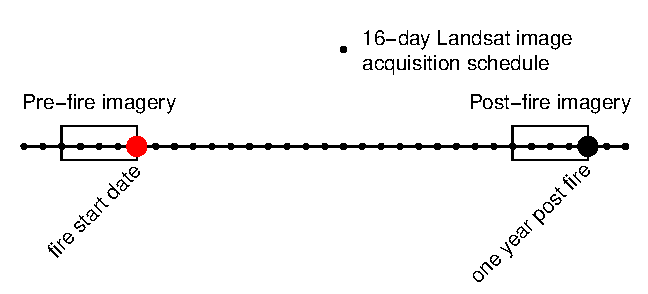
\includegraphics[width=6.00000in]{figure/chap01/image-acquisition-algorithm.pdf}
\caption{Schematic for how Landsat imagery was assembled in order to
make comparisons between pre- and post-fire conditions. This schematic
depicts a 64-day window of image collation prior to the fire which
comprise the pre-fire image collection. A similar, 64-day window
collection of imagery is assembled one year after the pre-fire image
collection.}
\end{figure}
\begin{figure}
\centering
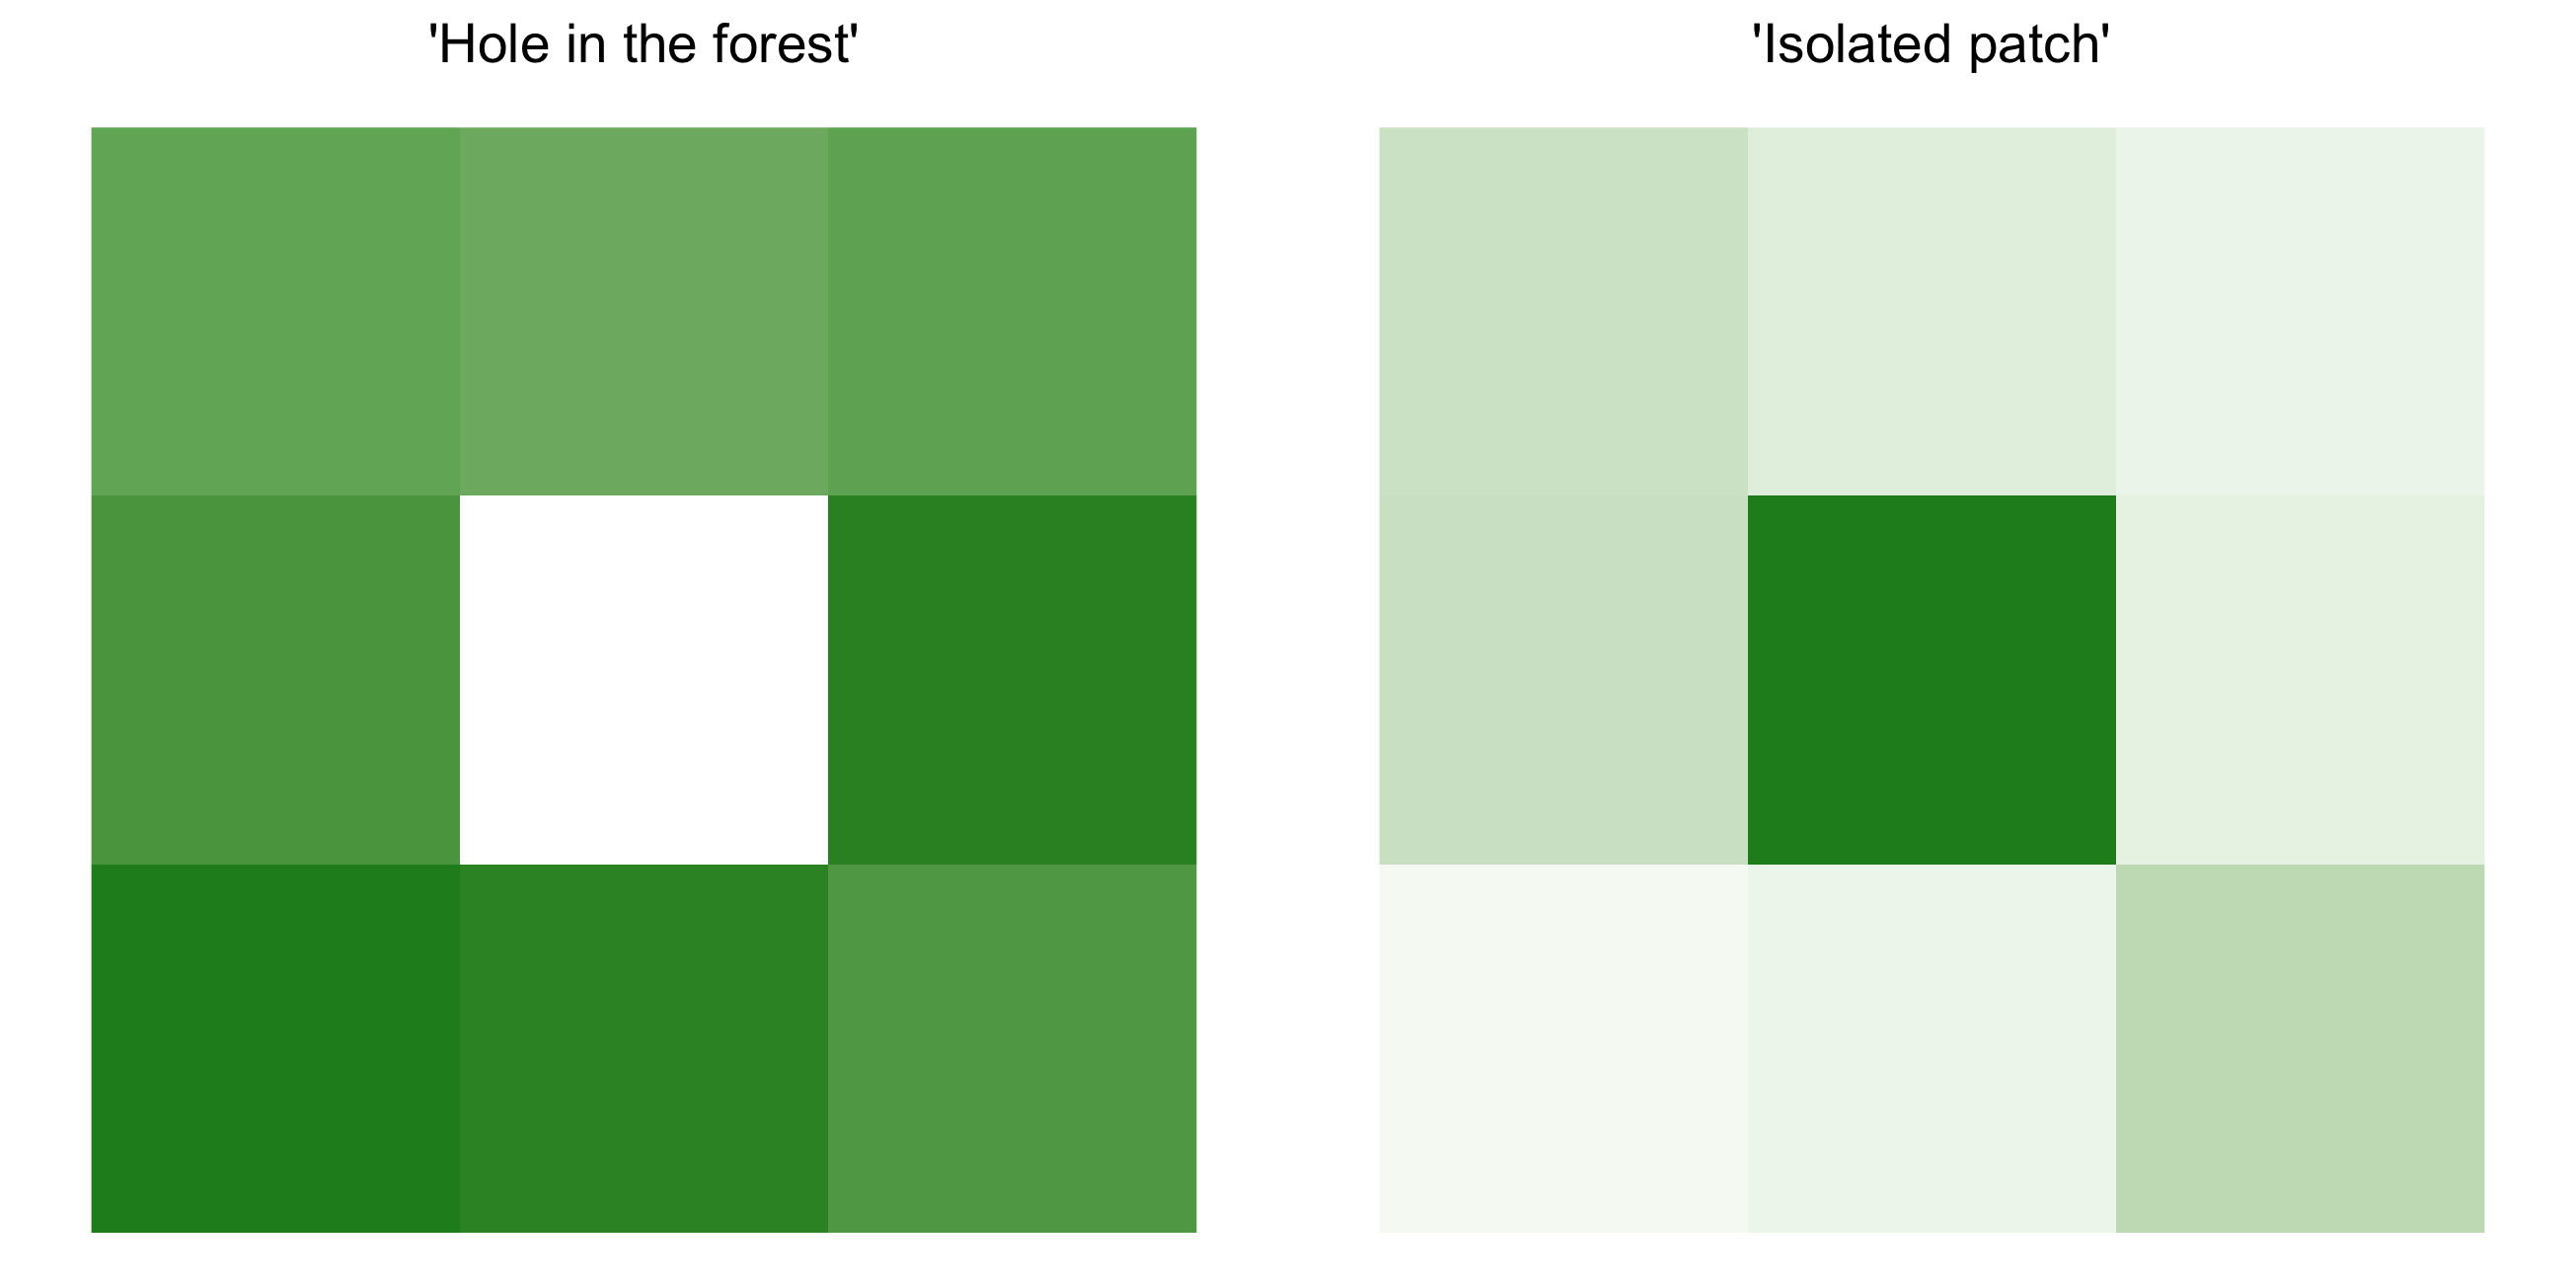
\includegraphics[width=6.00000in]{figure/chap01/decoupling-center-neighborhood-ndvi.png}
\caption{Conceptual diagram of `decoupling' that sometimes occurs
between the central pixel NDVI and the neighborhood mean NDVI. In each
of these scenarios, our model results suggest that the probability that
the central pixel burns at high severity is higher than expected given
the additive effect of the covariates. The left panel depicts the "hole
in the forest" decoupling, which occurs more frequently, and the right
panel depicts the "isolated patch" decoupling.}
\end{figure}
\backmatter

\chapter*{References}\label{references}
\addcontentsline{toc}{chapter}{References}

\markboth{References}{References}

\noindent

\setlength{\parindent}{-0.20in} \setlength{\leftskip}{0.20in}
\setlength{\parskip}{8pt}

\hypertarget{refs}{}
\hypertarget{ref-abatzoglou2013}{}
Abatzoglou, J. T. 2013. Development of gridded surface meteorological
data for ecological applications and modelling. International Journal of
Climatology 33:121--131.

\hypertarget{ref-abatzoglou2013a}{}
Abatzoglou, J. T., and C. A. Kolden. 2013. Relationships between climate
and macroscale area burned in the western United States. International
Journal of Wildland Fire 22:1003.

\hypertarget{ref-abatzoglou2016}{}
Abatzoglou, J. T., and A. P. Williams. 2016. Impact of anthropogenic
climate change on wildfire across western US forests. Proceedings of the
National Academy of Sciences 113:11770--11775.

\hypertarget{ref-abatzoglou2018a}{}
Abatzoglou, J. T., J. K. Balch, B. A. Bradley, and C. A. Kolden. 2018.
Human-related ignitions concurrent with high winds promote large
wildfires across the USA. International Journal of Wildland Fire
27:377--386.

\hypertarget{ref-ackerly2010}{}
Ackerly, D. D., S. R. Loarie, W. K. Cornwell, S. B. Weiss, H. Hamilton,
R. Branciforte, and N. J. B. Kraft. 2010. The geography of climate
change: Implications for conservation biogeography: Geography of climate
change. Diversity and Distributions 16:476--487.

\hypertarget{ref-agashe2009}{}
Agashe, D. 2009. The Stabilizing Effect of Intraspecific Genetic
Variation on Population Dynamics in Novel and Ancestral Habitats. The
American Naturalist 174:255--267.

\hypertarget{ref-agee2005}{}
Agee, J. K., and C. N. Skinner. 2005. Basic principles of forest fuel
reduction treatments. Forest Ecology and Management 211:83--96.

\hypertarget{ref-agee1996}{}
Agee, J., and C. ForestResourcesU. 1996. The influence of forest
structure on fire behavior. 17th Forest Vegetation Management
Conference:17.

\hypertarget{ref-anderegg2015a}{}
Anderegg, W. R. L., J. A. Hicke, R. A. Fisher, C. D. Allen, J. Aukema,
B. Bentz, S. Hood, J. W. Lichstein, A. K. Macalady, N. McDowell, Y. Pan,
K. Raffa, A. Sala, J. D. Shaw, N. L. Stephenson, C. Tague, and M.
Zeppel. 2015. Tree mortality from drought, insects, and their
interactions in a changing climate. New Phytologist 208:674--683.

\hypertarget{ref-asner2016}{}
Asner, G. P., P. G. Brodrick, C. B. Anderson, N. Vaughn, D. E. Knapp,
and R. E. Martin. 2016. Progressive forest canopy water loss during the
20122015 California drought. Proceedings of the National Academy of
Sciences 113:E249--E255.

\hypertarget{ref-baldwin2017a}{}
Baldwin, B. G., A. H. Thornhill, W. A. Freyman, D. D. Ackerly, M. M.
Kling, N. Morueta-Holme, and B. D. Mishler. 2017. Species richness and
endemism in the native flora of California. American Journal of Botany
104:487--501.

\hypertarget{ref-baskett2009}{}
Baskett, M. L., S. D. Gaines, and R. M. Nisbet. 2009. Symbiont diversity
may help coral reefs survive moderate climate change. Ecological
Applications 19:3--17.

\hypertarget{ref-bastarrika2011}{}
Bastarrika, A., E. Chuvieco, and M. P. Martín. 2011. Mapping burned
areas from Landsat TM/ETM+ data with a two-phase algorithm: Balancing
omission and commission errors. Remote Sensing of Environment
115:1003--1012.

\hypertarget{ref-beck2012}{}
Beck, J., L. Ballesteros-Mejia, C. M. Buchmann, J. Dengler, S. A. Fritz,
B. Gruber, C. Hof, F. Jansen, S. Knapp, H. Kreft, A.-K. Schneider, M.
Winter, and C. F. Dormann. 2012. What's on the horizon for macroecology?
Ecography 35:673--683.

\hypertarget{ref-bentz2010}{}
Bentz, B. J., J. Régnière, C. J. Fettig, E. M. Hansen, J. L. Hayes, J.
A. Hicke, R. G. Kelsey, J. F. Negrón, and S. J. Seybold. 2010. Climate
Change and Bark Beetles of the Western United States and Canada: Direct
and Indirect Effects. BioScience 60:602--613.

\hypertarget{ref-berryman1982}{}
Berryman, A. A. 1982. Population dynamics of bark beetles. Pages
264--314 \emph{in} Bark Beetles in North American Conifers: A System for
the Study of Evolutionary Biology.

\hypertarget{ref-boschetti2015}{}
Boschetti, L., D. P. Roy, C. O. Justice, and M. L. Humber. 2015.
MODISLandsat fusion for large area 30m burned area mapping. Remote
Sensing of Environment 161:27--42.

\hypertarget{ref-brooks1998}{}
Brooks, S. P., and A. Gelman. 1998. General Methods for Monitoring
Convergence of Iterative Simulations. Journal of Computational and
Graphical Statistics 7:434.

\hypertarget{ref-burkner2017}{}
Bürkner, P.-C. 2017. \textbf{Brms} : An \emph{R} Package for Bayesian
Multilevel Models Using \emph{Stan}. Journal of Statistical Software 80.

\hypertarget{ref-cadotte2013}{}
Cadotte, M., C. H. Albert, and S. C. Walker. 2013. The ecology of
differences: Assessing community assembly with trait and evolutionary
distances. Ecology Letters 16:1234--1244.

\hypertarget{ref-calkin2014}{}
Calkin, D. E., J. D. Cohen, M. A. Finney, and M. P. Thompson. 2014. How
risk management can prevent future wildfire disasters in the
wildland-urban interface. Proceedings of the National Academy of
Sciences 111:746--751.

\hypertarget{ref-calkin2005}{}
Calkin, D. E., K. M. Gebert, J. G. Jones, and R. P. Neilson. 2005.
Forest Service Large Fire Area Burned and Suppression Expenditure
Trends, 19702002. Journal of Forestry 103:179--183.

\hypertarget{ref-calkin2015}{}
Calkin, D. E., M. P. Thompson, and M. A. Finney. 2015. Negative
consequences of positive feedbacks in US wildfire management. Forest
Ecosystems. 2:9. doi: 10.1186/s40663-015-0033-8. 2.

\hypertarget{ref-cansler2012}{}
Cansler, C. A., and D. McKenzie. 2012. How Robust Are Burn Severity
Indices When Applied in a New Region? Evaluation of Alternate
Field-Based and Remote-Sensing Methods. Remote Sensing 4:456--483.

\hypertarget{ref-cansler2014}{}
Cansler, C. A., and D. McKenzie. 2014. Climate, fire size, and
biophysical setting control fire severity and spatial pattern in the
northern Cascade Range, USA. Ecological Applications 24:1037--1056.

\hypertarget{ref-chesson2000}{}
Chesson, P. 2000. Mechanisms of Maintenance of Species Diversity. Annual
Review of Ecology and Systematics 31:343--366.

\hypertarget{ref-chubaty2009}{}
Chubaty, A. M., B. D. Roitberg, and C. Li. 2009. A dynamic host
selection model for mountain pine beetle, Dendroctonus ponderosae
Hopkins. Ecological Modelling 220:1241--1250.

\hypertarget{ref-clark2016}{}
Clark, J. S., L. Iverson, C. W. Woodall, C. D. Allen, D. M. Bell, D. C.
Bragg, A. W. D'Amato, F. W. Davis, M. H. Hersh, I. Ibanez, S. T.
Jackson, S. Matthews, N. Pederson, M. Peters, M. W. Schwartz, K. M.
Waring, and N. E. Zimmermann. 2016. The impacts of increasing drought on
forest dynamics, structure, and biodiversity in the United States.
Global Change Biology 22:2329--2352.

\hypertarget{ref-clevers2013}{}
Clevers, J., and A. Gitelson. 2013. Remote estimation of crop and grass
chlorophyll and nitrogen content using red-edge bands on Sentinel-2 and
-3. International Journal of Applied Earth Observation and
Geoinformation 23:344--351.

\hypertarget{ref-coen2018}{}
Coen, J. L., E. N. Stavros, and J. A. Fites-Kaufman. 2018.
Deconstructing the King megafire. Ecological Applications 28:1565--1580.

\hypertarget{ref-collins2016}{}
Collins, B. M., J. M. Lydersen, D. L. Fry, K. Wilkin, T. Moody, and S.
L. Stephens. 2016. Variability in vegetation and surface fuels across
mixed-conifer-dominated landscapes with over 40 years of natural fire.
Forest Ecology and Management 381:74--83.

\hypertarget{ref-collins2017}{}
Collins, B. M., J. T. Stevens, J. D. Miller, S. L. Stephens, P. M.
Brown, and M. P. North. 2017. Alternative characterization of forest
fire regimes: Incorporating spatial patterns. Landscape Ecology
32:1543--1552.

\hypertarget{ref-coops2006}{}
Coops, N. C., M. Johnson, M. A. Wulder, and J. C. White. 2006.
Assessment of QuickBird high spatial resolution imagery to detect red
attack damage due to mountain pine beetle infestation. Remote Sensing of
Environment 103:67--80.

\hypertarget{ref-coppoletta2016}{}
Coppoletta, M., K. E. Merriam, and B. M. Collins. 2016. Post-fire
vegetation and fuel development influences fire severity patterns in
reburns. Ecological Applications 26:686--699.

\hypertarget{ref-crowther2015}{}
Crowther, T. W., H. B. Glick, K. R. Covey, C. Bettigole, D. S. Maynard,
S. M. Thomas, J. R. Smith, G. Hintler, M. C. Duguid, G. Amatulli, M.-N.
Tuanmu, W. Jetz, C. Salas, C. Stam, D. Piotto, R. Tavani, S. Green, G.
Bruce, S. J. Williams, S. K. Wiser, M. O. Huber, G. M. Hengeveld, G.-J.
Nabuurs, E. Tikhonova, P. Borchardt, C.-F. Li, L. W. Powrie, M. Fischer,
A. Hemp, J. Homeier, P. Cho, A. C. Vibrans, P. M. Umunay, S. L. Piao, C.
W. Rowe, M. S. Ashton, P. R. Crane, and M. A. Bradford. 2015. Mapping
tree density at a global scale. Nature 525:201--205.

\hypertarget{ref-dale2006}{}
Dale, L. 2006. Wildfire Policy and Fire Use on Public Lands in the
United States. Society \& Natural Resources 19:275--284.

\hypertarget{ref-davis1979}{}
Davis, J. B. 1979. A new fire management policy on Forest Service lands.
Fire Technology 15:43--50.

\hypertarget{ref-desantis2010}{}
De Santis, A., G. P. Asner, P. J. Vaughan, and D. E. Knapp. 2010.
Mapping burn severity and burning efficiency in California using
simulation models and Landsat imagery. Remote Sensing of Environment
114:1535--1545.

\hypertarget{ref-diffenbaugh2015}{}
Diffenbaugh, N. S., D. L. Swain, and D. Touma. 2015. Anthropogenic
warming has increased drought risk in California. Proceedings of the
National Academy of Sciences 112:3931--3936.

\hypertarget{ref-dillon2011}{}
Dillon, G. K., Z. A. Holden, P. Morgan, M. A. Crimmins, E. K. Heyerdahl,
and C. H. Luce. 2011. Both topography and climate affected forest and
woodland burn severity in two regions of the western US, 1984 to 2006.
Ecosphere 2:art130.

\hypertarget{ref-dji2015}{}
DJI. 2015a. Zenmuse X3 - Creativity Unleashed.
\url{https://www.dji.com/zenmuse-x3/info}.

\hypertarget{ref-dji2015a}{}
DJI. 2015b. DJI - The World Leader in Camera Drones/Quadcopters for
Aerial Photography. \url{https://www.dji.com/matrice100/info}.

\hypertarget{ref-doane2006}{}
Doane, D., J. O'Laughlin, P. Morgan, and C. Miller. 2006. Barriers to
wildland fire use 12:3.

\hypertarget{ref-dronesmadeeasy2018}{}
DronesMadeEasy. 2018. ‎Map Pilot for DJI on iOS.
\url{https://itunes.apple.com/us/app/map-pilot-for-dji/id1014765000?mt=8}.

\hypertarget{ref-earles2014}{}
Earles, J. M., M. P. North, and M. D. Hurteau. 2014. Wildfire and
drought dynamics destabilize carbon stores of fire-suppressed forests.
Ecological Applications. 24(4): 732-740 24:732--740.

\hypertarget{ref-edwards2018}{}
Edwards, A. C., J. Russell-Smith, and S. W. Maier. 2018. A comparison
and validation of satellite-derived fire severity mapping techniques in
fire prone north Australian savannas: Extreme fires and tree stem
mortality. Remote Sensing of Environment 206:287--299.

\hypertarget{ref-eidenshink2007}{}
Eidenshink, J., B. Schwind, K. Brewer, Z.-L. Zhu, B. Quayle, and S.
Howard. 2007. A Project for Monitoring Trends in Burn Severity. Fire
Ecology 3:3--21.

\hypertarget{ref-evenden2014}{}
Evenden, M. L., C. M. Whitehouse, and J. Sykes. 2014. Factors
Influencing Flight Capacity of the Mountain Pine Beetle (Coleoptera:
Curculionidae: Scolytinae). Environmental Entomology 43:187--196.

\hypertarget{ref-eysn2015}{}
Eysn, L., M. Hollaus, E. Lindberg, F. Berger, J.-M. Monnet, M. Dalponte,
M. Kobal, M. Pellegrini, E. Lingua, D. Mongus, and N. Pfeifer. 2015. A
Benchmark of Lidar-Based Single Tree Detection Methods Using
Heterogeneous Forest Data from the Alpine Space. Forests 6:1721--1747.

\hypertarget{ref-farr2007}{}
Farr, T. G., P. A. Rosen, E. Caro, R. Crippen, R. Duren, S. Hensley, M.
Kobrick, M. Paller, E. Rodriguez, L. Roth, D. Seal, S. Shaffer, J.
Shimada, J. Umland, M. Werner, M. Oskin, D. Burbank, and D. Alsdorf.
2007. The Shuttle Radar Topography Mission. Reviews of Geophysics 45.

\hypertarget{ref-fernandez-garcia2018}{}
Fernández-García, V., M. Santamarta, A. Fernández-Manso, C. Quintano, E.
Marcos, and L. Calvo. 2018. Burn severity metrics in fire-prone pine
ecosystems along a climatic gradient using Landsat imagery. Remote
Sensing of Environment 206:205--217.

\hypertarget{ref-fettig2012b}{}
Fettig, C. J. 2012. Chapter 2: Forest health and bark beetles. \emph{in}
Managing Sierra Nevada Forests. PSW-GTR-237. USDA Forest Service.

\hypertarget{ref-fettig2007}{}
Fettig, C. J., K. D. Klepzig, R. F. Billings, A. S. Munson, T. E.
Nebeker, J. F. Negrón, and J. T. Nowak. 2007. The effectiveness of
vegetation management practices for prevention and control of bark
beetle infestations in coniferous forests of the western and southern
United States. Forest Ecology and Management 238:24--53.

\hypertarget{ref-fettig2019}{}
Fettig, C. J., L. A. Mortenson, B. M. Bulaon, and P. B. Foulk. 2019.
Tree mortality following drought in the central and southern Sierra
Nevada, California, U.S. Forest Ecology and Management 432:164--178.

\hypertarget{ref-flint2013}{}
Flint, L. E., A. L. Flint, J. H. Thorne, and R. Boynton. 2013.
Fine-scale hydrologic modeling for regional landscape applications: The
California Basin Characterization Model development and performance.
Ecological Processes 2:25.

\hypertarget{ref-floyd2009}{}
Floyd, M. L., M. Clifford, N. S. Cobb, D. Hanna, R. Delph, P. Ford, and
D. Turner. 2009. Relationship of stand characteristics to
drought-induced mortality in three Southwestern piñonJuniper woodlands.
Ecological Applications 19:1223--1230.

\hypertarget{ref-foga2017}{}
Foga, S., P. L. Scaramuzza, S. Guo, Z. Zhu, R. D. Dilley, T. Beckmann,
G. L. Schmidt, J. L. Dwyer, M. Joseph Hughes, and B. Laue. 2017. Cloud
detection algorithm comparison and validation for operational Landsat
data products. Remote Sensing of Environment 194:379--390.

\hypertarget{ref-franklin1986}{}
Franklin, J., T. Logan, C. Woodcock, and A. Strahler. 1986. Coniferous
Forest Classification and Inventory Using Landsat and Digital Terrain
Data. IEEE Transactions on Geoscience and Remote Sensing GE-24:139--149.

\hypertarget{ref-frey2018}{}
Frey, J., K. Kovach, S. Stemmler, and B. Koch. 2018. UAV Photogrammetry
of Forests as a Vulnerable Process. A Sensitivity Analysis for a
Structure from Motion RGB-Image Pipeline. Remote Sensing 10:912.

\hypertarget{ref-fried2004}{}
Fried, J. S., M. S. Torn, and E. Mills. 2004. The Impact of Climate
Change on Wildfire Severity: A Regional Forecast for Northern
California. Climatic Change 64:169--191.

\hypertarget{ref-fule1997}{}
Fulé, P. Z., W. W. Covington, and M. M. Moore. 1997. Determining
Reference Conditions for Ecosystem Management of Southwestern Ponderosa
Pine Forests. Ecological Applications 7:895--908.

\hypertarget{ref-gabry2019}{}
Gabry, J., D. Simpson, A. Vehtari, M. Betancourt, and A. Gelman. 2019.
Visualization in Bayesian workflow. Journal of the Royal Statistical
Society: Series A (Statistics in Society) 182:389--402.

\hypertarget{ref-gao1996}{}
Gao, B.-c. 1996. NDWIA normalized difference water index for remote
sensing of vegetation liquid water from space. Remote Sensing of
Environment 58:257--266.

\hypertarget{ref-garcia1991}{}
García, M. L., and V. Caselles. 1991. Mapping burns and natural
reforestation using thematic Mapper data. Geocarto International
6:31--37.

\hypertarget{ref-gazol2016}{}
Gazol, A., and J. J. Camarero. 2016. Functional diversity enhances
silver fir growth resilience to an extreme drought. Journal of Ecology
104:1063--1075.

\hypertarget{ref-gelman2018}{}
Gelman, A., B. Goodrich, J. Gabry, and A. Vehtari. 2018. R-squared for
Bayesian regression models. The American Statistician:1--6.

\hypertarget{ref-gitelson1994}{}
Gitelson, A., and M. N. Merzlyak. 1994. Spectral Reflectance Changes
Associated with Autumn Senescence of Aesculus hippocastanum L. and Acer
platanoides L. Leaves. Spectral Features and Relation to Chlorophyll
Estimation. Journal of Plant Physiology 143:286--292.

\hypertarget{ref-goodwin2014}{}
Goodwin, N. R., and L. J. Collett. 2014. Development of an automated
method for mapping fire history captured in Landsat TM and ETM+ time
series across Queensland, Australia. Remote Sensing of Environment
148:206--221.

\hypertarget{ref-gorelick2017}{}
Gorelick, N., M. Hancher, M. Dixon, S. Ilyushchenko, D. Thau, and R.
Moore. 2017. Google Earth Engine: Planetary-scale geospatial analysis
for everyone. Remote Sensing of Environment 202:18--27.

\hypertarget{ref-graf2012}{}
Graf, M., M. Reid, B. Aukema, and B. Lindgren. 2012. Association of tree
diameter with body size and lipid content of mountain pine beetles. The
Canadian Entomologist 144:467--477.

\hypertarget{ref-graham2004}{}
Graham, R. T., S. McCaffrey, and T. B. Jain. 2004. Science basis for
changing forest structure to modify wildfire behavior and severity. U.S.
Department of Agriculture, Forest Service, Rocky Mountain Research
Station, Ft. Collins, CO.

\hypertarget{ref-gray2019}{}
Gray, P. C., A. B. Fleishman, D. J. Klein, M. W. McKown, V. S. Bézy, K.
J. Lohmann, and D. W. Johnston. 2019. A convolutional neural network for
detecting sea turtles in drone imagery. Methods in Ecology and Evolution
10:345--355.

\hypertarget{ref-griffin2014}{}
Griffin, D., and K. J. Anchukaitis. 2014. How unusual is the 20122014
California drought? Geophysical Research Letters 41:9017--9023.

\hypertarget{ref-hansen2013}{}
Hansen, M. C., P. V. Potapov, R. Moore, M. Hancher, S. A. Turubanova, A.
Tyukavina, D. Thau, S. V. Stehman, S. J. Goetz, T. R. Loveland, A.
Kommareddy, A. Egorov, L. Chini, C. O. Justice, and J. R. G. Townshend.
2013. High-Resolution Global Maps of 21st-Century Forest Cover Change.
Science 342:850--853.

\hypertarget{ref-haralick1973}{}
Haralick, R. M., K. Shanmugam, and I. Dinstein. 1973. Textural Features
for Image Classification. IEEE Transactions on Systems, Man, and
Cybernetics SMC-3:610--621.

\hypertarget{ref-harvey2016b}{}
Harvey, B. J., D. C. Donato, and M. G. Turner. 2016. Drivers and trends
in landscape patterns of stand-replacing fire in forests of the US
Northern Rocky Mountains (1984-2010). Landscape Ecology 31:2367--2383.

\hypertarget{ref-hawbaker2017}{}
Hawbaker, T. J., M. K. Vanderhoof, Y.-J. Beal, J. D. Takacs, G. L.
Schmidt, J. T. Falgout, B. Williams, N. M. Fairaux, M. K. Caldwell, J.
J. Picotte, S. M. Howard, S. Stitt, and J. L. Dwyer. 2017. Mapping
burned areas using dense time-series of Landsat data. Remote Sensing of
Environment 198:504--522.

\hypertarget{ref-hayes2009}{}
Hayes, C. J., C. J. Fettig, and L. D. Merrill. 2009. Evaluation of
Multiple Funnel Traps and Stand Characteristics for Estimating Western
Pine Beetle-Caused Tree Mortality. Journal of Economic Entomology
102:2170--2182.

\hypertarget{ref-heffernan2014}{}
Heffernan, J. B., P. A. Soranno, M. J. Angilletta, L. B. Buckley, D. S.
Gruner, T. H. Keitt, J. R. Kellner, J. S. Kominoski, A. V. Rocha, J.
Xiao, T. K. Harms, S. J. Goring, L. E. Koenig, W. H. McDowell, H.
Powell, A. D. Richardson, C. A. Stow, R. Vargas, and K. C. Weathers.
2014. Macrosystems ecology: Understanding ecological patterns and
processes at continental scales. Frontiers in Ecology and the
Environment 12:5--14.

\hypertarget{ref-henry2019}{}
Henry, L., and H. Wickham. 2019. Purrr: Functional Programming Tools.

\hypertarget{ref-hijmans2019}{}
Hijmans, R. J., J. van Etten, M. Sumner, J. Cheng, A. Bevan, R. Bivand,
L. Busetto, M. Canty, D. Forrest, A. Ghosh, D. Golicher, J. Gray, J. A.
Greenberg, P. Hiemstra, I. for M. A. Geosciences, C. Karney, M.
Mattiuzzi, S. Mosher, J. Nowosad, E. Pebesma, O. P. Lamigueiro, E. B.
Racine, B. Rowlingson, A. Shortridge, B. Venables, and R. Wueest. 2019.
Raster: Geographic Data Analysis and Modeling.

\hypertarget{ref-hoffman2014}{}
Hoffman, M. D., and A. Gelman. 2014. The No-U-Turn Sampler: Adaptively
Setting Path Lengths in Hamiltonian Monte Carlo. Journal of Machine
Learning Research 15:31.

\hypertarget{ref-holden2009}{}
Holden, Z. A., P. Morgan, and J. S. Evans. 2009. A predictive model of
burn severity based on 20-year satellite-inferred burn severity data in
a large southwestern US wilderness area. Forest Ecology and Management
258:2399--2406.

\hypertarget{ref-holling1973}{}
Holling, C. S. 1973. Resilience and Stability of Ecological Systems.
Annual Review of Ecology and Systematics:1--23.

\hypertarget{ref-houtman2013}{}
Houtman, R. M., C. A. Montgomery, A. R. Gagnon, D. E. Calkin, T. G.
Dietterich, S. McGregor, and M. Crowley. 2013. Allowing a wildfire to
burn: Estimating the effect on future fire suppression costs.
International Journal of Wildland Fire 22:871--882.

\hypertarget{ref-huang2014}{}
Huang, Q., A. Swatantran, R. Dubayah, and S. J. Goetz. 2014. The
Influence of Vegetation Height Heterogeneity on Forest and Woodland Bird
Species Richness across the United States. PLoS ONE 9:e103236.

\hypertarget{ref-huesca2016}{}
Huesca, M., M. García, K. L. Roth, A. Casas, and S. L. Ustin. 2016.
Canopy structural attributes derived from AVIRIS imaging spectroscopy
data in a mixed broadleaf/conifer forest. Remote Sensing of Environment
182:208--226.

\hypertarget{ref-hunziker2017}{}
Hunziker, P. 2017. Velox: Fast Raster Manipulation and Extraction.

\hypertarget{ref-jakubowski2013}{}
Jakubowski, M. K., W. Li, Q. Guo, and M. Kelly. 2013. Delineating
Individual Trees from Lidar Data: A Comparison of Vector- and
Raster-based Segmentation Approaches. Remote Sensing 5:4163--4186.

\hypertarget{ref-janzen1998}{}
Janzen, F. J., and H. S. Stern. 1998. Logistic Regression for Empirical
Studies of Multivariate Selection. Evolution 52:1564--1571.

\hypertarget{ref-jepsonfloraproject2016}{}
JepsonFloraProject, editor. 2016. Jepson eFlora.

\hypertarget{ref-johnson2009}{}
Johnson, J. F., D. N. Bengston, and D. P. Fan. 2009. US Policy Response
to the Wildfire Fuels Management Problem: An Analysis of the News Media
Debate about the Healthy Forests Initiative and the Healthy Forests
Restoration Act. Journal of Environmental Policy \& Planning
11:129--142.

\hypertarget{ref-kane2014}{}
Kane, V. R., M. P. North, J. A. Lutz, D. J. Churchill, S. L. Roberts, D.
F. Smith, R. J. McGaughey, J. T. Kane, and M. L. Brooks. 2014. Assessing
fire effects on forest spatial structure using a fusion of Landsat and
airborne LiDAR data in Yosemite National Park. Remote Sensing of
Environment 151:89--101.

\hypertarget{ref-keane2002a}{}
Keane, R. E., K. C. Ryan, T. T. Veblen, C. D. Allen, J. Logan, and B.
Hawkes. 2002. Cascading Effects of Fire Exclusion in Rocky Mountain
Ecosystems : A Literature Review. Page 24. USDA Forest Service, Rocky
Mountain Research Station.

\hypertarget{ref-keeley2009}{}
Keeley, J. E. 2009. Fire intensity, fire severity and burn severity: A
brief review and suggested usage. International Journal of Wildland Fire
18:116.

\hypertarget{ref-keith2013}{}
Keith, D. A., J. P. Rodríguez, K. M. Rodríguez-Clark, E. Nicholson, K.
Aapala, A. Alonso, M. Asmussen, S. Bachman, A. Basset, E. G. Barrow, J.
S. Benson, M. J. Bishop, R. Bonifacio, T. M. Brooks, M. A. Burgman, P.
Comer, F. A. Comín, F. Essl, D. Faber-Langendoen, P. G. Fairweather, R.
J. Holdaway, M. Jennings, R. T. Kingsford, R. E. Lester, R. M. Nally, M.
A. McCarthy, J. Moat, M. A. Oliveira-Miranda, P. Pisanu, B. Poulin, T.
J. Regan, U. Riecken, M. D. Spalding, and S. Zambrano-Martínez. 2013.
Scientific Foundations for an IUCN Red List of Ecosystems. PLoS ONE
8:e62111.

\hypertarget{ref-key2006}{}
Key, C. H., and N. C. Benson. 2006. Landscape Assessment (LA):55.

\hypertarget{ref-kefi2014}{}
Kéfi, S., V. Guttal, W. A. Brock, S. R. Carpenter, A. M. Ellison, V. N.
Livina, D. A. Seekell, M. Scheffer, E. H. van Nes, and V. Dakos. 2014.
Early Warning Signals of Ecological Transitions: Methods for Spatial
Patterns. PLoS ONE 9:e92097.

\hypertarget{ref-kolb2016}{}
Kolb, T. E., C. J. Fettig, M. P. Ayres, B. J. Bentz, J. A. Hicke, R.
Mathiasen, J. E. Stewart, and A. S. Weed. 2016. Observed and anticipated
impacts of drought on forest insects and diseases in the United States.
Forest Ecology and Management 380:321--334.

\hypertarget{ref-kolden2015}{}
Kolden, C. A., A. M. S. Smith, and J. T. Abatzoglou. 2015. Limitations
and utilisation of Monitoring Trends in Burn Severity products for
assessing wildfire severity in the USA. International Journal of
Wildland Fire 24:1023.

\hypertarget{ref-koontz2019}{}
Koontz, M. J., S. E. Fick, C. M. Werner, M. P. North, and A. M. Latimer.
2019a. Wildfire severity, vegetation characteristics, and regional
climate for fires covering more than 4 hectares burning in yellow
pine/mixed-conifer forests of the Sierra Nevada, California, USA from
1984 to 2017. Open Science Framework.

\hypertarget{ref-koontz2019a}{}
Koontz, M. J., M. P. North, C. M. Werner, S. E. Fick, and A. M. Latimer.
2019b. Local variability of vegetation structure increases forest
resilience to wildfire. EcoEvoRxiv.

\hypertarget{ref-kotliar1990}{}
Kotliar, N. B., and J. A. Wiens. 1990. Multiple Scales of Patchiness and
Patch Structure: A Hierarchical Framework for the Study of
Heterogeneity. Oikos 59:253.

\hypertarget{ref-kuhn2008}{}
Kuhn, M. 2008. Building Predictive Models in R Using the caret Package.
Journal of Statistical Software 28:1--26.

\hypertarget{ref-lande1983}{}
Lande, R., and S. J. Arnold. 1983. THE MEASUREMENT OF SELECTION ON
CORRELATED CHARACTERS. Evolution 37:1210--1226.

\hypertarget{ref-larson2012}{}
Larson, A. J., and D. Churchill. 2012. Tree spatial patterns in
fire-frequent forests of western North America, including mechanisms of
pattern formation and implications for designing fuel reduction and
restoration treatments. Forest Ecology and Management 267:74--92.

\hypertarget{ref-lenoir2013}{}
Lenoir, J., B. J. Graae, P. A. Aarrestad, I. G. Alsos, W. S. Armbruster,
G. Austrheim, C. Bergendorff, H. J. B. Birks, K. A. Bråthen, J. Brunet,
H. H. Bruun, C. J. Dahlberg, G. Decocq, M. Diekmann, M. Dynesius, R.
Ejrnaes, J.-A. Grytnes, K. Hylander, K. Klanderud, M. Luoto, A. Milbau,
M. Moora, B. Nygaard, A. Odland, V. T. Ravolainen, S. Reinhardt, S. M.
Sandvik, F. H. Schei, J. D. M. Speed, L. U. Tveraabak, V. Vandvik, L. G.
Velle, R. Virtanen, M. Zobel, and J.-C. Svenning. 2013. Local
temperatures inferred from plant communities suggest strong spatial
buffering of climate warming across Northern Europe. Global Change
Biology 19:1470--1481.

\hypertarget{ref-li2012}{}
Li, W., Q. Guo, M. K. Jakubowski, and M. Kelly. 2012. A New Method for
Segmenting Individual Trees from the Lidar Point Cloud. Photogrammetric
Engineering \& Remote Sensing 78:75--84.

\hypertarget{ref-logan1998}{}
Logan, J. A., P. White, B. J. Bentz, and J. A. Powell. 1998. Model
Analysis of Spatial Patterns in Mountain Pine Beetle Outbreaks.
Theoretical Population Biology 53:236--255.

\hypertarget{ref-lydersen2015}{}
Lydersen, J. M., B. M. Collins, E. E. Knapp, G. B. Roller, and S.
Stephens. 2015. Relating fuel loads to overstorey structure and
composition in a fire-excluded Sierra Nevada mixed conifer forest.
International Journal of Wildland Fire 24:484.

\hypertarget{ref-lydersen2014}{}
Lydersen, J. M., M. P. North, and B. M. Collins. 2014. Severity of an
uncharacteristically large wildfire, the Rim Fire, in forests with
relatively restored frequent fire regimes. Forest Ecology and Management
328:326--334.

\hypertarget{ref-lydersen2013}{}
Lydersen, J. M., M. P. North, E. E. Knapp, and B. M. Collins. 2013.
Quantifying spatial patterns of tree groups and gaps in mixed-conifer
forests: Reference conditions and long-term changes following fire
suppression and logging. Forest Ecology and Management 304:370--382.

\hypertarget{ref-mallek2013}{}
Mallek, C., H. Safford, J. Viers, and J. Miller. 2013. Modern departures
in fire severity and area vary by forest type, Sierra Nevada and
southern Cascades, California, USA. Ecosphere 4:art153.

\hypertarget{ref-malone2018}{}
Malone, S., P. Fornwalt, M. Battaglia, M. Chambers, J. Iniguez, and C.
Sieg. 2018. Mixed-Severity Fire Fosters Heterogeneous Spatial Patterns
of Conifer Regeneration in a Dry Conifer Forest. Forests 9:45.

\hypertarget{ref-mann2015}{}
Mann, M. E., and P. H. Gleick. 2015. Climate change and California
drought in the 21st century. Proceedings of the National Academy of
Sciences 112:3858--3859.

\hypertarget{ref-masek2006}{}
Masek, J., E. Vermote, N. Saleous, R. Wolfe, F. Hall, K. Huemmrich, F.
Gao, J. Kutler, and T.-K. Lim. 2006. A Landsat Surface Reflectance
Dataset for North America, 19902000. IEEE Geoscience and Remote Sensing
Letters 3:68--72.

\hypertarget{ref-mccune2007}{}
McCune, B. 2007. Improved estimates of incident radiation and heat load
using non- parametric regression against topographic variables. Journal
of Vegetation Science 18:751--754.

\hypertarget{ref-mccune2002}{}
McCune, B., and D. Keon. 2002. Equations for potential annual direct
incident radiation and heat load. Journal of Vegetation Science
13:603--606.

\hypertarget{ref-mckenzie2008}{}
McKenzie, D., and A. E. Hessl. 2008. A neutral model of low-severity
fire regimes. In: Narog, Marcia G., tech. coord. 2008. Proceedings of
the 2002 Fire Conference: Managing fire and fuels in the remaining
wildlands and open spaces of the Southwestern United States. Gen. Tech.
Rep. PSW-GTR-189. Albany, CA: U.S. Department of Agriculture, Forest
Service, Pacific Southwest Research Station. p. 139-150 189:139--150.

\hypertarget{ref-meyer1990}{}
Meyer, F., and S. Beucher. 1990. Morphological segmentation. Journal of
Visual Communication and Image Representation 1:21--46.

\hypertarget{ref-meyer2015}{}
Meyer, M. D. 2015. Forest Fire Severity Patterns of Resource Objective
Wildfires in the Southern Sierra Nevada. Journal of Forestry 113:49--56.

\hypertarget{ref-micasense2015}{}
Micasense. 2015. MicaSense.
\url{https://support.micasense.com/hc/en-us/articles/215261448-RedEdge-User-Manual-PDF-Download-}.

\hypertarget{ref-millar2015}{}
Millar, C. I., and N. L. Stephenson. 2015. Temperate forest health in an
era of emerging megadisturbance. Science 349:823--826.

\hypertarget{ref-millar2007}{}
Millar, C. I., N. L. Stephenson, and S. L. Stephens. 2007. CLIMATE
CHANGE AND FORESTS OF THE FUTURE: MANAGING IN THE FACE OF UNCERTAINTY.
Ecological Applications 17:2145--2151.

\hypertarget{ref-millar2012}{}
Millar, C. I., R. D. Westfall, D. L. Delany, M. J. Bokach, A. L. Flint,
and L. E. Flint. 2012. Forest mortality in high-elevation whitebark pine
( \emph{Pinus} \emph{Albicaulis} ) forests of eastern California, USA;
influence of environmental context, bark beetles, climatic water
deficit, and warming. Canadian Journal of Forest Research 42:749--765.

\hypertarget{ref-miller2012a}{}
Miller, J. D., and H. Safford. 2012. TRENDS IN WILDFIRE SEVERITY: 1984
TO2010 IN THE SIERRA NEVADA, MODOC PLATEAU, AND SOUTHERN CASCADES,
CALIFORNIA, USA. Fire Ecology 8:41--57.

\hypertarget{ref-miller2017}{}
Miller, J. D., and H. D. Safford. 2017. Corroborating Evidence of a
Pre-Euro-American Low- to Moderate-Severity Fire Regime in Yellow
PineMixed Conifer Forests of the Sierra Nevada, California, USA. Fire
Ecology 13:58--90.

\hypertarget{ref-miller2007}{}
Miller, J. D., and A. E. Thode. 2007. Quantifying burn severity in a
heterogeneous landscape with a relative version of the delta Normalized
Burn Ratio (dNBR). Remote Sensing of Environment 109:66--80.

\hypertarget{ref-miller2009a}{}
Miller, J. D., E. E. Knapp, C. H. Key, C. N. Skinner, C. J. Isbell, R.
M. Creasy, and J. W. Sherlock. 2009. Calibration and validation of the
relative differenced Normalized Burn Ratio (RdNBR) to three measures of
fire severity in the Sierra Nevada and Klamath Mountains, California,
USA. Remote Sensing of Environment 113:645--656.

\hypertarget{ref-miller2012}{}
Miller, J. D., C. N. Skinner, H. D. Safford, E. E. Knapp, and C. M.
Ramirez. 2012. Trends and causes of severity, size, and number of fires
in northwestern California, USA. Ecological Applications 22:184--203.

\hypertarget{ref-miller1960}{}
Miller, J. M., and F. P. Keen. 1960. Biology and control of the western
pine beetle: A summary of the first fifty years of research. US
Department of Agriculture.

\hypertarget{ref-moeck1981}{}
Moeck, H. A., D. L. Wood, and K. Q. Lindahl. 1981. Host selection
behavior of bark beetles (Coleoptera: Scolytidae) attackingPinus
ponderosa, with special emphasis on the western pine beetle,Dendroctonus
brevicomis. Journal of Chemical Ecology 7:49--83.

\hypertarget{ref-moritz2005}{}
Moritz, M. A., M. E. Morais, L. A. Summerell, J. M. Carlson, and J.
Doyle. 2005. Wildfires, complexity, and highly optimized tolerance.
Proceedings of the National Academy of Sciences 102:17912--17917.

\hypertarget{ref-morris2017}{}
Morris, J. L., S. Cottrell, C. J. Fettig, W. D. Hansen, R. L. Sherriff,
V. A. Carter, J. L. Clear, J. Clement, R. J. DeRose, J. A. Hicke, P. E.
Higuera, K. M. Mattor, A. W. R. Seddon, H. T. Seppä, J. D. Stednick, and
S. J. Seybold. 2017. Managing bark beetle impacts on ecosystems and
society: Priority questions to motivate future research. Journal of
Applied Ecology 54:750--760.

\hypertarget{ref-north2015}{}
North, M. P., S. L. Stephens, B. M. Collins, J. K. Agee, G. Aplet, J. F.
Franklin, and P. Z. Fule. 2015. Reform forest fire management. Science
349:1280--1281.

\hypertarget{ref-north2009a}{}
North, M., P. Stine, K. O'Hara, W. Zielinski, and S. Stephens. 2009. An
ecosystem management strategy for Sierran mixed-conifer forests. U.S.
Department of Agriculture, Forest Service, Pacific Southwest Research
Station, Albany, CA.

\hypertarget{ref-parks2018}{}
Parks, S. A., L. M. Holsinger, M. H. Panunto, W. M. Jolly, S. Z.
Dobrowski, and G. K. Dillon. 2018. High-severity fire: Evaluating its
key drivers and mapping its probability across western US forests.
Environmental Research Letters 13:044037.

\hypertarget{ref-parks2014a}{}
Parks, S., G. Dillon, and C. Miller. 2014. A New Metric for Quantifying
Burn Severity: The Relativized Burn Ratio. Remote Sensing 6:1827--1844.

\hypertarget{ref-pau2010}{}
Pau, G., F. Fuchs, O. Sklyar, M. Boutros, and W. Huber. 2010. EBImagean
R package for image processing with applications to cellular phenotypes.
Bioinformatics 26:979--981.

\hypertarget{ref-pebesma2018}{}
Pebesma, E. 2018. Simple Features for R: Standardized Support for
Spatial Vector Data. The R Journal.

\hypertarget{ref-pebesma2019b}{}
Pebesma, E. 2019a. Stars: Spatiotemporal Arrays, Raster and Vector Data
Cubes.

\hypertarget{ref-pebesma2019a}{}
Pebesma, E. 2019b. Lwgeom: Bindings to Selected 'liblwgeom' Functions
for Simple Features.

\hypertarget{ref-pebesma2019}{}
Pebesma, E., R. Bivand, E. Racine, M. Sumner, I. Cook, T. Keitt, R.
Lovelace, H. Wickham, J. Ooms, K. Müller, and T. L. Pedersen. 2019. Sf:
Simple Features for R.

\hypertarget{ref-peters2004}{}
Peters, D. P. C., R. A. Pielke, B. T. Bestelmeyer, C. D. Allen, S.
Munson-McGee, and K. M. Havstad. 2004. Cross-scale interactions,
nonlinearities, and forecasting catastrophic events. Proceedings of the
National Academy of Sciences 101:15130--15135.

\hypertarget{ref-pile2019}{}
Pile, L. S., M. D. Meyer, R. Rojas, O. Roe, and M. T. Smith. 2019.
Drought Impacts and Compounding Mortality on Forest Trees in the
Southern Sierra Nevada. Forests 10:237.

\hypertarget{ref-plowright2018a}{}
Plowright, A. 2018a. APfun: Geo-Processing Helper Functions.

\hypertarget{ref-plowright2018}{}
Plowright, A. 2018b. ForestTools: Analyzing Remotely Sensed Forest Data.

\hypertarget{ref-popescu2004}{}
Popescu, S. C., and R. H. Wynne. 2004. Seeing the Trees in the Forest:
Using Lidar and Multispectral Data Fusion with Local Filtering and
Variable Window Size for Estimating Tree Height. PHOTOGRAMMETRIC
ENGINEERING:16.

\hypertarget{ref-preisler2017}{}
Preisler, H. K., N. E. Grulke, Z. Heath, and S. L. Smith. 2017. Analysis
and out-year forecast of beetle, borer, and drought-induced tree
mortality in California. Forest Ecology and Management. 399: 166-178
399:166--178.

\hypertarget{ref-prichard2014}{}
Prichard, S. J., and M. C. Kennedy. 2014. Fuel treatments and landform
modify landscape patterns of burn severity in an extreme fire event.
Ecological Applications 24:571--590.

\hypertarget{ref-questad2008}{}
Questad, E. J., and B. L. Foster. 2008. Coexistence through
spatio-temporal heterogeneity and species sorting in grassland plant
communities. Ecology Letters 11:717--726.

\hypertarget{ref-rcoreteam2018}{}
R Core Team. 2018. R: A Language and Environment for Statistical
Computing. R Foundation for Statistical Computing, Vienna, Austria.

\hypertarget{ref-raffa1983}{}
Raffa, K. F., and A. A. Berryman. 1983. The Role of Host Plant
Resistance in the Colonization Behavior and Ecology of Bark Beetles
(Coleoptera: Scolytidae). Ecological Monographs 53:27--49.

\hypertarget{ref-raffa1987}{}
Raffa, K. F., and A. A. Berryman. 1987. Interacting Selective Pressures
in Conifer-Bark Beetle Systems: A Basis for Reciprocal Adaptations? The
American Naturalist 129:234--262.

\hypertarget{ref-raffa2008}{}
Raffa, K. F., B. H. Aukema, B. J. Bentz, A. L. Carroll, J. A. Hicke, M.
G. Turner, and W. H. Romme. 2008. Cross-scale Drivers of Natural
Disturbances Prone to Anthropogenic Amplification: The Dynamics of Bark
Beetle Eruptions. BioScience 58:501--517.

\hypertarget{ref-raffa2015}{}
Raffa, K. F., J.-C. Grégoire, and B. Staffan Lindgren. 2015. Natural
History and Ecology of Bark Beetles. Pages 1--40 \emph{in} Bark Beetles.
Elsevier.

\hypertarget{ref-reilly2017}{}
Reilly, M. J., C. J. Dunn, G. W. Meigs, T. A. Spies, R. E. Kennedy, J.
D. Bailey, and K. Briggs. 2017. Contemporary patterns of fire extent and
severity in forests of the Pacific Northwest, USA (1985-2010). Ecosphere
8:e01695.

\hypertarget{ref-reusch2005}{}
Reusch, T. B. H., A. Ehlers, A. Hammerli, and B. Worm. 2005. Ecosystem
recovery after climatic extremes enhanced by genotypic diversity.
Proceedings of the National Academy of Sciences 102:2826--2831.

\hypertarget{ref-ross2018}{}
Ross, N. 2018. Fasterize: Fast Polygon to Raster Conversion.

\hypertarget{ref-rouse1973}{}
Rouse, W., R. H. Haas, W. Deering, and J. A. Schell. 1973. MONITORING
THE VERNAL ADVANCEMENT AND RETROGRADATION (GREEN WAVE EFFECT) OF NATURAL
VEGETATION. Type II Report, Goddard Space Flight Center, Greenbelt, MD,
USA.

\hypertarget{ref-roussel2019a}{}
Roussel, J.-R. 2019. lidRplugins: Extra functions and algorithms for
lidR package.

\hypertarget{ref-roussel2019}{}
Roussel, J.-R., D. A. (. the documentation), F. D. B. (. bugs and
improved catalog features), and A. S. M. (. lassnags). 2019. lidR:
Airborne LiDAR Data Manipulation and Visualization for Forestry
Applications.

\hypertarget{ref-safford2017}{}
Safford, H. D., and J. T. Stevens. 2017. Natural Range of Variation for
Yellow Pine and Mixed-Conifer Forests in the Sierra Nevada, Southern
Cascades, and Modoc and Inyo National Forests, California, USA. Page
241.

\hypertarget{ref-safford2012}{}
Safford, H., J. Stevens, K. Merriam, M. Meyer, and A. Latimer. 2012.
Fuel treatment effectiveness in California yellow pine and mixed conifer
forests. Forest Ecology and Management 274:17--28.

\hypertarget{ref-scholl2010}{}
Scholl, A. E., and A. H. Taylor. 2010. Fire regimes, forest change, and
self-organization in an old-growth mixed-conifer forest, Yosemite
National Park, USA. Ecological Applications 20:362--380.

\hypertarget{ref-schweizer2014}{}
Schweizer, D., and R. Cisneros. 2014. Wildland fire management and air
quality in the southern Sierra Nevada: Using the Lion Fire as a case
study with a multi-year perspective on PM2.5 impacts and fire policy.
Journal of Environmental Management 144:265--278.

\hypertarget{ref-seidl2016a}{}
Seidl, R., J. Müller, T. Hothorn, C. Bässler, M. Heurich, and M. Kautz.
2016. Small beetle, large-scale drivers: How regional and landscape
factors affect outbreaks of the European spruce bark beetle. The Journal
of applied ecology 53:530--540.

\hypertarget{ref-shiklomanov2019}{}
Shiklomanov, A. N., B. A. Bradley, K. M. Dahlin, A. M. Fox, C. M. Gough,
F. M. Hoffman, E. M. Middleton, S. P. Serbin, L. Smallman, and W. K.
Smith. 2019. Enhancing global change experiments through integration of
remote-sensing techniques. Frontiers in Ecology and the Environment 0.

\hypertarget{ref-shin2018}{}
Shin, P., T. Sankey, M. Moore, and A. Thode. 2018. Evaluating Unmanned
Aerial Vehicle Images for Estimating Forest Canopy Fuels in a Ponderosa
Pine Stand. Remote Sensing 10:1266.

\hypertarget{ref-short2017}{}
Short, K. C. 2017. Spatial wildfire occurrence data for the United
States, 1992-2015 {[}FPA\_FOD\_20170508{]} (4th Edition).

\hypertarget{ref-sikkink2013}{}
Sikkink, P. G., G. K. Dillon, R. E. Keane, P. Morgan, E. C. Karau, Z. A.
Holden, and R. P. Silverstein. 2013. Composite Burn Index (CBI) data and
field photos collected for the FIRESEV project, western United States.

\hypertarget{ref-steel2018}{}
Steel, Z. L., M. J. Koontz, and H. D. Safford. 2018. The changing
landscape of wildfire: Burn pattern trends and implications for
California's yellow pine and mixed conifer forests. Landscape Ecology
33:1159--1176.

\hypertarget{ref-steel2015}{}
Steel, Z. L., H. D. Safford, and J. H. Viers. 2015. The fire
frequency-severity relationship and the legacy of fire suppression in
California forests. Ecosphere 6:art8.

\hypertarget{ref-stein2014}{}
Stein, A., K. Gerstner, and H. Kreft. 2014. Environmental heterogeneity
as a universal driver of species richness across taxa, biomes and
spatial scales. Ecology Letters 17:866--880.

\hypertarget{ref-stephens2018}{}
Stephens, S. L., B. M. Collins, C. J. Fettig, M. A. Finney, C. M.
Hoffman, E. E. Knapp, M. P. North, H. Safford, and R. B. Wayman. 2018.
Drought, Tree Mortality, and Wildfire in Forests Adapted to Frequent
Fire. BioScience 68:77--88.

\hypertarget{ref-stephens2008}{}
Stephens, S. L., D. L. Fry, and E. Franco-Vizcaíno. 2008. Wildfire and
Spatial Patterns in Forests in Northwestern Mexico: The United States
Wishes It Had Similar Fire Problems. Ecology and Society 13.

\hypertarget{ref-stephens2012a}{}
Stephens, S. L., J. D. McIver, R. E. J. Boerner, C. J. Fettig, J. B.
Fontaine, B. R. Hartsough, P. L. Kennedy, and D. W. Schwilk. 2012. The
Effects of Forest Fuel-Reduction Treatments in the United States.
BioScience 62:549--560.

\hypertarget{ref-stephens2009}{}
Stephens, S. L., J. J. Moghaddas, C. Edminster, C. E. Fiedler, S. Haase,
M. Harrington, J. E. Keeley, E. E. Knapp, J. D. McIver, K. Metlen, C. N.
Skinner, and A. Youngblood. 2009. Fire treatment effects on vegetation
structure, fuels, and potential fire severity in western U.S. forests.
Ecological Applications 19:305--320.

\hypertarget{ref-stephenson1998}{}
Stephenson, N. 1998. Actual evapotranspiration and deficit: Biologically
meaningful correlates of vegetation distribution across spatial scales.
Journal of Biogeography 25:855--870.

\hypertarget{ref-stephenson2019}{}
Stephenson, N. L., A. J. Das, N. J. Ampersee, and B. M. Bulaon. 2019.
Which trees die during drought? The key role of insect host-tree
selection. Journal of Ecology:75.

\hypertarget{ref-stevens2017}{}
Stevens, J. T., B. M. Collins, J. D. Miller, M. P. North, and S. L.
Stephens. 2017. Changing spatial patterns of stand-replacing fire in
California conifer forests. Forest Ecology and Management 406:28--36.

\hypertarget{ref-stevens-rumann2018}{}
Stevens-Rumann, C. S., K. B. Kemp, P. E. Higuera, B. J. Harvey, M. T.
Rother, D. C. Donato, P. Morgan, and T. T. Veblen. 2018. Evidence for
declining forest resilience to wildfires under climate change. Ecology
Letters 21:243--252.

\hypertarget{ref-sugihara2006}{}
Sugihara, N. G., J. W. V. Wagtendonk, J. Fites-Kaufman, K. E. Shaffer,
and A. E. Thode. 2006. Fire in California's ecosystems. University of
California Press.

\hypertarget{ref-thistle2004}{}
Thistle, H. W., H. Peterson, G. Allwine, B. Lamb, T. Strand, E. H.
Holsten, and P. J. Shea. 2004. Surrogate Pheromone Plumes in Three
Forest Trunk Spaces: Composite Statistics and Case Studies. Forest
Science 50.

\hypertarget{ref-tilman1994}{}
Tilman, D. 1994. Competition and Biodiversity in Spatially Structured
Habitats. Ecology 75:2--16.

\hypertarget{ref-trumbore2015}{}
Trumbore, S., P. Brando, and H. Hartmann. 2015. Forest health and global
change. Science 349:814--818.

\hypertarget{ref-tuanmu2015}{}
Tuanmu, M.-N., and W. Jetz. 2015. A global, remote sensing-based
characterization of terrestrial habitat heterogeneity for biodiversity
and ecosystem modelling: Global habitat heterogeneity. Global Ecology
and Biogeography 24:1329--1339.

\hypertarget{ref-usdafs2019}{}
USDAFS. 2019, February 11. Press Release: Survey finds 18 million trees
died in California in 2018.
\url{https://www.fs.usda.gov/Internet/FSE_DOCUMENTS/FSEPRD609321.pdf}.

\hypertarget{ref-usgs2017a}{}
USGS. 2017a. Landsat 8 Surface Reflectance Code (LASRC) Product
Guide:40.

\hypertarget{ref-usgs2017}{}
USGS. 2017b. Landsat 4-7 Surface Reflectance (LEDAPS) Product Guide:41.

\hypertarget{ref-veblen2000}{}
Veblen, T. T., T. Kitzberger, and J. Donnegan. 2000. Climatic and Human
Influences on Fire Regimes in Ponderosa Pine Forests in the Colorado
Front Range. Ecological Applications 10:1178--1195.

\hypertarget{ref-vega2014}{}
Vega, C., A. Hamrouni, S. El Mokhtari, J. Morel, J. Bock, J. P. Renaud,
M. Bouvier, and S. Durrieu. 2014. PTrees: A point-based approach to
forest tree extraction from lidar data. International Journal of Applied
Earth Observation and Geoinformation 33:98--108.

\hypertarget{ref-vehtari2017}{}
Vehtari, A., A. Gelman, and J. Gabry. 2017. Practical Bayesian model
evaluation using leave-one-out cross-validation and WAIC. Statistics and
Computing 27:1413--1432.

\hypertarget{ref-veraverbeke2013}{}
Veraverbeke, S., and S. J. Hook. 2013. Evaluating spectral indices and
spectral mixture analysis for assessing fire severity, combustion
completeness and carbon emissions. International Journal of Wildland
Fire 22:707.

\hypertarget{ref-vermote2016}{}
Vermote, E., C. Justice, M. Claverie, and B. Franch. 2016. Preliminary
analysis of the performance of the Landsat 8/OLI land surface
reflectance product. Remote Sensing of Environment 185:46--56.

\hypertarget{ref-virah-sawmy2009}{}
Virah-Sawmy, M., L. Gillson, and K. J. Willis. 2009. How does spatial
heterogeneity influence resilience to climatic changes? Ecological
dynamics in southeast Madagascar. Ecological Monographs 79:557--574.

\hypertarget{ref-wagner1977}{}
Wagner, C. E. V. 1977. Conditions for the start and spread of crown
fire. Canadian Journal of Forest Research 7:23--34.

\hypertarget{ref-wagtendonk2006}{}
Wagtendonk, J. W. V. 2006. Fire as a Physical Process. University of
California Press.

\hypertarget{ref-walker2004}{}
Walker, B., C. S. Holling, S. R. Carpenter, and A. P. Kinzig. 2004.
Resilience, Adaptability and Transformability in Social-ecological
Systems. Ecology and Society 9.

\hypertarget{ref-walker2018}{}
Walker, R. B., J. D. Coop, S. A. Parks, and L. Trader. 2018. Fire
regimes approaching historic norms reduce wildfire-facilitated
conversion from forest to non-forest. Ecosphere 9:e02182.

\hypertarget{ref-welch2016}{}
Welch, K. R., H. D. Safford, and T. P. Young. 2016. Predicting conifer
establishment post wildfire in mixed conifer forests of the North
American Mediterranean-climate zone. Ecosphere 7:e01609.

\hypertarget{ref-westerling2006}{}
Westerling, A. L. 2006. Warming and Earlier Spring Increase Western U.S.
Forest Wildfire Activity. Science 313:940--943.

\hypertarget{ref-westerling2016}{}
Westerling, A. L. 2016. Increasing western US forest wildfire activity:
Sensitivity to changes in the timing of spring. Philosophical
Transactions of the Royal Society B: Biological Sciences 371:20150178.

\hypertarget{ref-white1997}{}
White, P., and J. Powell. 1997. Phase transition from environmental to
dynamic determinism in mountain pine beetle attack. Bulletin of
Mathematical Biology 59:609--643.

\hypertarget{ref-wickham2017}{}
Wickham, H. 2017. Tidyverse: Easily Install and Load the 'Tidyverse'.

\hypertarget{ref-wickham2019}{}
Wickham, H. 2019. Modelr: Modelling Functions that Work with the Pipe.

\hypertarget{ref-parkwilliams2013}{}
Williams, A. P., C. D. Allen, A. K. Macalady, D. Griffin, C. A.
Woodhouse, D. M. Meko, T. W. Swetnam, S. A. Rauscher, R. Seager, H. D.
Grissino-Mayer, J. S. Dean, E. R. Cook, C. Gangodagamage, M. Cai, and N.
G. McDowell. 2013. Temperature as a potent driver of regional forest
drought stress and tree mortality. Nature Climate Change 3:292--297.

\hypertarget{ref-wood2012}{}
Wood, E. M., A. M. Pidgeon, V. C. Radeloff, and N. S. Keuler. 2012.
Image texture as a remotely sensed measure of vegetation structure.
Remote Sensing of Environment 121:516--526.

\hypertarget{ref-young2017}{}
Young, D. J. N., J. T. Stevens, J. M. Earles, J. Moore, A. Ellis, A. L.
Jirka, and A. M. Latimer. 2017. Long-term climate and competition
explain forest mortality patterns under extreme drought. Ecology Letters
20:78--86.

\hypertarget{ref-young2019}{}
Young, D. J. N., C. M. Werner, K. R. Welch, T. P. Young, H. D. Safford,
and A. M. Latimer. 2019. Post-fire forest regeneration shows limited
climate tracking and potential for drought-induced type conversion.
Ecology 100:e02571.

\hypertarget{ref-zhang2016}{}
Zhang, W., J. Qi, P. Wan, H. Wang, D. Xie, X. Wang, and G. Yan. 2016. An
Easy-to-Use Airborne LiDAR Data Filtering Method Based on Cloth
Simulation. Remote Sensing 8:501.

\hypertarget{ref-zhu2006}{}
Zhu, Z., C. Key, D. Ohlen, and N. Benson. 2006. Evaluate Sensitivities
of Burn-Severity Mapping Algorithms for Different Ecosystems and Fire
Histories in the United States. Page 35. Final Report to the Joint Fire
Science Program.

\end{ucmainmatter}
\end{document}

%---Set Headers and Footers ------------------------------------------------------
\pagestyle{fancy}
\renewcommand{\chaptermark}[1]{\markboth{{\sf #1 \hspace*{\fill} Chapter~\thechapter}}{} }
\renewcommand{\sectionmark}[1]{\markright{ {\sf Section~\thesection \hspace*{\fill} #1 }}}
\fancyhf{}

\makeatletter \if@twoside \fancyhead[LO]{\small \rightmark} \fancyhead[RE]{\small\leftmark} \else \fancyhead[LO]{\small\leftmark}
\fancyhead[RE]{\small\rightmark} \fi

\def\cleardoublepage{\clearpage\if@openright \ifodd\c@page\else
  \hbox{}
  \vspace*{\fill}
  \begin{center}
    This page intentionally left blank
  \end{center}
  \vspace{\fill}
  \thispagestyle{plain}
  \newpage
  \fi \fi}
  
\makeatother
\fancyfoot[c]{\textrm{\textup{\thepage}}} % page number
\fancyfoot[C]{\thepage}
\renewcommand{\headrulewidth}{0.4pt}

\fancypagestyle{plain} { \fancyhf{} \fancyfoot[C]{\thepage}
\renewcommand{\headrulewidth}{0pt}
\renewcommand{\footrulewidth}{0pt}}

